\chapter{\mFourL: A measurement designed for re-interpretation}
\label{chap:fourlepton}

<<<<<<< HEAD
 %% m4l motivation
\section{Motivation for the \mFourL measurement}
\label{sec:fourlepmotivation}

The four lepton channel is a particularly interesting channel to study as it receives contributions from many physics processes.  

First and foremost, there is the production of a pair of \PZ-bosons via quark-antiquark interactions in \info[]{s-channel not in SM because it includes neutral ZZZ or ZZ\photon vertex} both the \Ptop- and \Pup-channel. The \Ptop-channel diagram is shown in Figure \ref{fig:m4lfeynman:qqZZ}, and represents, by far, \improvement[]{Read more about why the u-channel diagram is not preferred} the largest contribution to the \ZZ production and thus to the \mFourL distribution. At the low mass end where $\mFourL=m_{PZ}$, there is resonant production of a single \PZ boson via the s-channel diagram in Figure \ref{fig:m4lfeynman:singleZ}. At $\mFourL=\unit{180}{\GeV}$ and beyond, the threshold for the on-shell production of two \PZ bosons is reached and results in a peak in the four lepton invariant mass spectrum. 

Second in magnitude is the gluon-induced production of a \PZ boson pair. This occurs via a triangle or box quark loop, which results in a factor $\alpha_s^2$ suppression. It still plays a substantial role, however, because at small $x$\footnote{Here $x$ is the component of the proton's momentum carried by the struck quark. At the \LHC the protons have very high energies; therefore the \LHC can be described as a small $x$ collider \cite{zotov2012small}} gluon-gluon luminosity is higher than the quark-antiquark luminosity \cite{Glover:194539}. The contribution from this process in on the order of ten percent \cite{Becker:2230817}. Finally in the pool of \PZ boson pairs there is a small contribution from decaying Higgs bosons, which themselves are produced also via gluon fusion, as illustrated in Figure \ref{fig:m4lfeynman:ggHZZ}. There is resonant Higgs production at \mFourL=\unit{125}{\GeV}, and a non-resonant enhancement at $\mFourL=m_{\Ptop}=\unit{350}{\GeV}$ from the top quark loop. Beyond \unit{350}{\GeV}, the Higgs-mediated \PZ boson pair production process destructively interferes with continuum production of on-shell \PZ bosons \cite{Campbell_2016}.

The \mFourL distribution can be a useful probe for certain new physics scenarios. Take for example, the high mass tail of the invariant mass spectrum. This region is dependent on the couplings of the Higgs to incoming and outgoing particles while independent of the Higgs boson width \cite{Campbell_2016}, a unique property that can be exploited to derive model-independent limits on the Higgs couplings, and on the \todo{reword, this is copy pasted} contribution of new states in the Higgs to gluon coupling \cite{Cacciapaglia_2014}. It has also been previously exploited to derive model-independent constraints on the Higgs boson width \cite{Caola_2013}. 

%% Secondly, under specific assumptions a class of models exists for which the off-shell coupling measurement together with a measurement of the on-shell signal strength can be re-interpreted in terms of a bound on the total Higgs boson width. In this paper, we provide a first step towards a classification of the models for which a total width measurement is viable and we discuss examples of BSM models for which the off-shell coupling measurement can be important in either constraining or even discovering new physics in the upcoming LHC runs

\begin{figure}
    \centering
    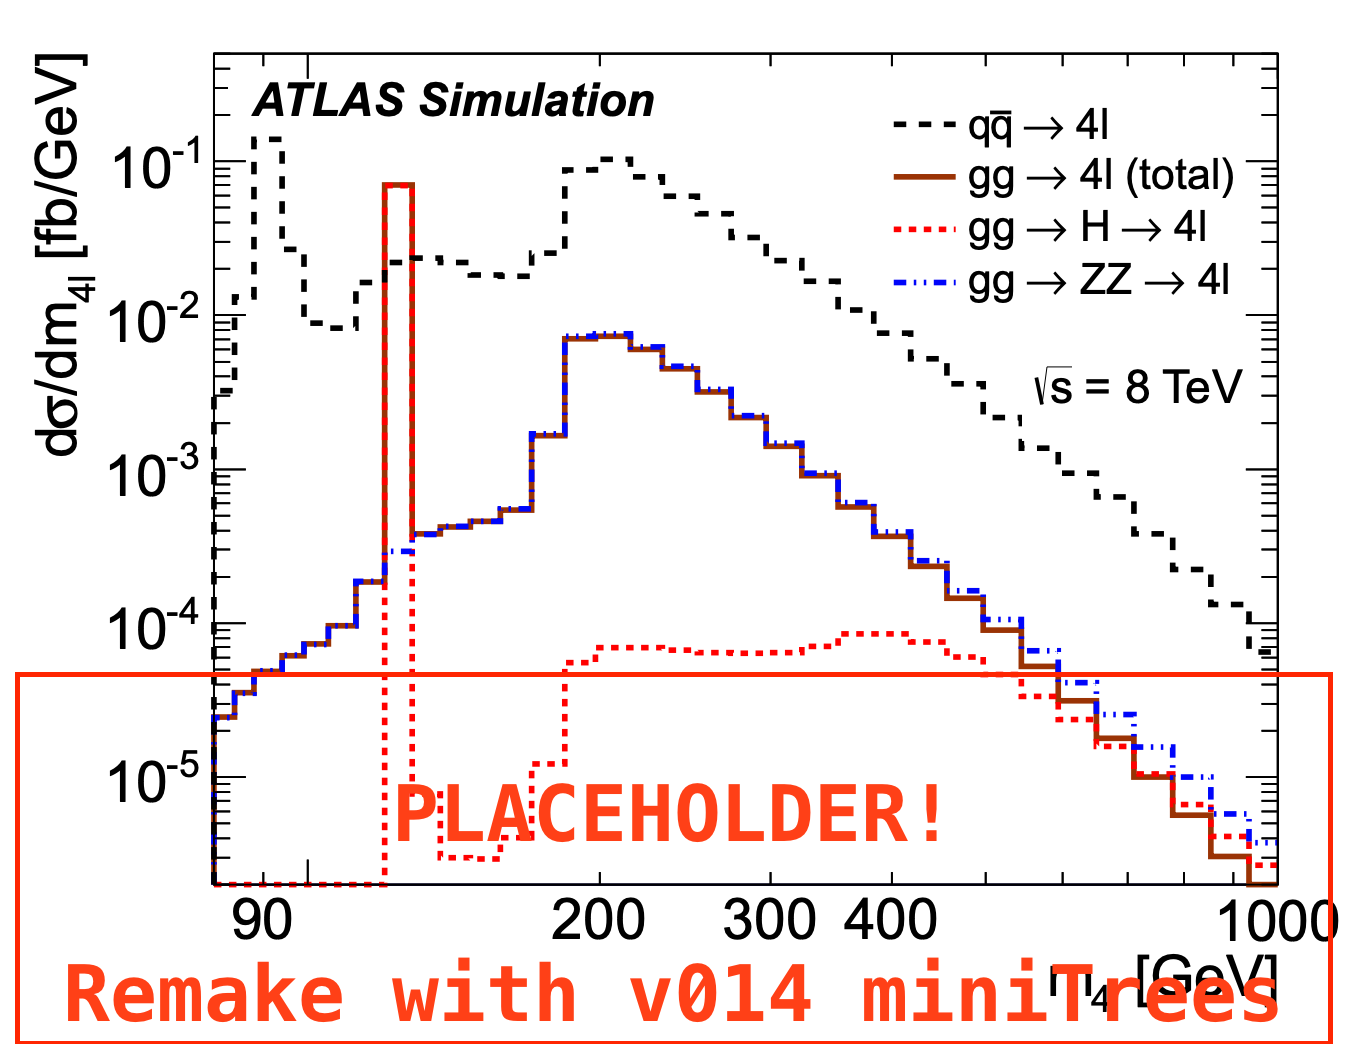
\includegraphics[width=0.5\textwidth]{Figures/m4l/m4lbreakdown.png}
    \caption{Breakdown of contributing processes contributing to the \mFourL distribution.}
    \todo[inline]{Replace and remake with our miniTrees.}
    \label{fig:m4lbreakdown}
\end{figure}

\begin{figure}
\centering
\begin{subfigure}{.24\textwidth}
  \centering
  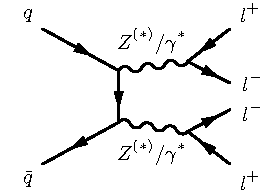
\includegraphics[width=.23\textwidth]{Figures/FeynGraphs/qqZZ4l.pdf}
  \caption{\qqZZ}
  \label{fig:m4lfeynman:qqZZ}
\end{subfigure}%
\begin{subfigure}{.24\textwidth}
  \centering
  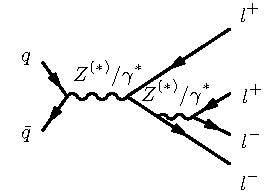
\includegraphics[width=.23\textwidth]{Figures/FeynGraphs/qqZZ4lrad.pdf}
  \caption{A subfigure}
  \label{fig:m4lfeynman:singleZ}
\end{subfigure}
\begin{subfigure}{.24\textwidth}
  \centering
  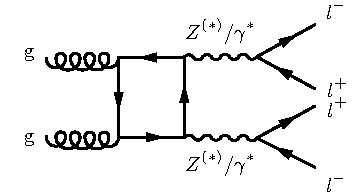
\includegraphics[width=.23\textwidth]{Figures/FeynGraphs/ggZZ4lbox.pdf}
  \caption{A subfigure}
  \label{fig:m4lfeynman:ggZZ}
\end{subfigure}
\begin{subfigure}{.24\textwidth}
  \centering
  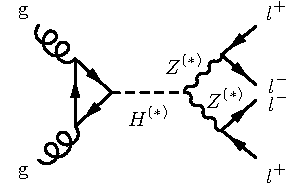
\includegraphics[width=.23\textwidth]{Figures/FeynGraphs/ggZZ4lhiggs.pdf}
  \caption{A subfigure}
  \label{fig:m4lfeynman:ggHZZ}
\end{subfigure}
\caption{Feynman diagrams for quark- and gluon-induced \ZZ production. The processes shown are the main contributors.}
\label{fig:m4lfeynman}
\end{figure}

% this channel provides a clean leptonic final state resulting in a small instrumental background, where one or more of the reconstructed lepton candidates originate from the misidentification of jet fragments or from nonprompt leptons.

 %% Signal definition and event selection
\section{Signal and fiducial region definition}
\label{sec:signaldef}

The motivation behind this analysis is to make a measurement as inclusive and as model-independent as possible. Any process leading to a final state of four lepton - made up of two same flavour opposite sign electron or muon pairs - is considered to be part of the signal. Electrons or muons originating from fully leptonic decays of taus are counted towards the signal. 

The fiducial region definition follows closely the acceptance of the detector. Furthermore, by loosening the mass cuts, there is higher event acceptance especially in the low mass regions. Preliminary studies were conducted to investigate the impact of loosening and simplifying the dilepton lower mass cut to \unit{5}{\GeV} and removing the upper mass cut, for example, as opposed to the varying higher cuts in the previous round of the analysis. Unsurprisingly, these result in a higher event yield in both the low and high mass tails of the \mFourL distribution. 

The final state is defined solely in terms of final state particles as opposed to targeting a specific process. Beyond the requirement of two same flavour opposite sign lepton pairs, the measurement is inclusive to additional particles such as additional leptons, jets, and invisible particles. Previous irreducible backgrounds (\VVV, \ttZ) are now considered as part of the signal since they produce four or more prompt leptons.

\missingfigure{Emily plots for loosening mass cuts}

\subsection{Lepton definitions}

For particle physicists, a prompt lepton simply means the lepton did not originate from a hadron. Prompt leptons are further classified into three categories depending on their association with emitted photons. These three categories are:
\begin{itemize}
    \item Born leptons: leptons prior to QED Final State Radiation (FSR);
    \item Bare leptons: leptons after QED FSR;
    \item Dressed leptons: leptons after QED FSR, that then have the four momenta of nearby radiated photons added to it. 
\end{itemize}
The ATLAS detector makes lepton measurements after QED FSR has occurred. It is for this reason that born leptons are not the best choice. It is more realistic to perform measurements involving only final state particles, and objects constructed from final state particles, such as dressed leptons \cite{Kar:ab1be6}. 

\subsubsection{Dressed electrons and bare muons}

In this analysis, a choice of dressing electrons but leaving muons bare was made to closer mimic what is seen by the detector. 

%% Truth isolation
When selecting leptons in the data, there is a complex isolation criteria applied \todo[]{What is this isolation criteria?}. An emulation of this reconstruction-level criteria is included in the fiducial region definition. Although the particle-level application is a simplification, it nevertheless returns a result that is closer to what is actually measured. The particle-level truth isolation criteria requires the sum of the transverse momentum of all charged particles inside a $\Delta R  = 0.3$ cone of the lepton, divided by transverse momentum of the lepton itself, to be less than 0.16. If any other selected leptons are within the cone, their
momenta is not included. 
$$\dfrac{\pt(\Delta R  = 0.3)}{\pt(\text{lepton})}<0.16$$
\subsection{Fiducial region}

\begin{table}[bp]
  \begin{tabular}{lllll}
        & Lepton requirements \\
        \midrule
        Electrons & Dressed lepton definition\\
                & \pt > \unit{5}{\GeV}\\
                & $|\eta| < 2.47$\\
        Muons & Bare lepton definition\\
            & \pt > \unit{7}{\GeV}\\
            & $|\eta| < 2.7$\\
        \bottomrule
        \toprule
        & Event requirements \\
        \midrule
            Four-lepton signature & At least 4 leptons, with 2 Same-Flavour, Opposite-Sign pairs \\
               Lepton kinematics   &   $\pt > 20 / 10$~\GeV{} for
                                     leading two leptons \\ [0.3cm]
              Lepton separation               &   $\Delta R_{ij} > 0.05$ for any leptons \\
              $J/\psi$-Veto &    $  m_{ij} > 5$~\GeV for all SFOS pairs \\
              Truth isolation & ptcone30/\pt < 0.16 \\
  \end{tabular}
  \caption{Fiducial region definition.}
  \label{tab:fidregion}
\end{table}

\missingfigure[]{Dressed electrons, bare muons plot}

\subsection*{Lepton pairing and quadruplet formation} 
\todo[inline]{Reword this whole subsection!!}
Events satisfying the requirements described above enter the fiducial region of the measurement. 
In order to define observables, a unique set of exactly four leptons per event is chosen: 
\begin{itemize}
\item First, the SFOS lepton pair with an invariant mass closest to the Z boson mass is selected as the primary pair in the event. 
\item The remaining SFOS lepton pair closest to the Z boson mass is then referred to as the secondary pair, and completes the quadruplet. 
\end{itemize}
In this way, only one quadruplet is defined even in events containing more than four leptons.
This selection strategy is chosen since it prefers to form pairs that correspond to on-shell Z bosons for the dominant $ZZ$ pair production process, making the pair-level observables based on this definition comparable to such obtained in dedicated $ZZ$ production measurements. This is explored further in Appendix~\ref{app:pairing}. 
The pair and quadruplet formation does not have any impact on the event selection outcome. 

\section{Measured observables}

The star observable of the analysis is none other than the four lepton invariant mass, \mFourL. It has been measured previously by both the \ATLAS and the \CMS experiment \todo{missing citation} \cite{}. As with the previous round of the analysis, the \mFourL distribution is also measured double-differentially, in slices of the transverse momentum of the four lepton system, the absolute rapidity of the four lepton system, and the flavour channel of the four lepton system. 

New to this round of the analysis is the division of the four lepton invariant mass spectrum into four separate regions, each dominated by a different process. From \unit{60}{\GeV}-\unit{100}{\GeV} resonant single \Z production reigns, similarly the \unit{120}{\GeV}-\unit{130}{\GeV} region is dominated by Higgs production, and the high mass region from \unit{180}{\GeV}-\unit{2000}{\GeV} by on-shell \ZZ production. Lastly to fill the gaps between  \unit{20}{\GeV}-\unit{60}{\GeV}, \unit{100}{\GeV}-\unit{120}{\GeV}, and \unit{130}{\GeV}-\unit{180}{\GeV} is the off-shell \ZZ region. This is summarised in Table \ref{tab:m4lregions}. The following variables are measured double differentially in these four regions:

\begin{itemize}
    \item Cosine of angle $\theta^{*}$, where $\theta^{*}$ is the angle between the \todo{definitely check this} lepton in the rest frame and the \Z boson in the lab frame. This angle is sensitive to the polarisation of the decaying boson.
    \item The difference in rapidity between the lepton pairs
    \item The difference in azimuthal angle between the lepton pairs, and between leading leptons
    \item The invariant mass of the lepton pairs
    \item The transverse momentum of the lepton pairs
\end{itemize}

\begin{table}[bp]
  \begin{tabular}{lllll}
        Region & \mFourL interval(s) \\
        \midrule
        \ZFourL & \unit{60}{\GeV} < \mFourL < \unit{100}{\GeV} \\
        \HFourL & \unit{120}{\GeV} < \mFourL < \unit{130}{\GeV} \\
        On-shell \ZZ & \unit{180}{\GeV} < \mFourL < \unit{2000}{\GeV} \\
        Off-shell \ZZ & \unit{20}{\GeV} < \mFourL < \unit{60}{\GeV}, \unit{100}{\GeV} < \mFourL < \unit{120}{\GeV}, \\
          & and \unit{130}{\GeV} < \mFourL < \unit{180}{\GeV}\\
  \end{tabular}
  \caption{The four \mFourL regions dominated by the single \Z, Higgs, on-shell and off-shell \ZZ processes.}
  \label{tab:m4lregions}
\end{table}

 \section{Event reconstruction and selection}
\label{sec:eventselection}
A critical aspect of any analysis is its event selection. The dominant backgrounds are shaped by the selection choices, and signal sensitivity are enhanced with optimized cuts. The objective of the selection in this analysis is to efficiently identify the four lepton final states while keeping the background at a minimum. This is achieved through a combination of online trigger (described in detail in Section \ref{ssec:ATLAStrigger}) and offline event selection cuts. As with all \ATLAS analysis, basic requirements on the event cleaning are imposed. Only data recorded with stable beam conditions and with all relevant information from sub-detectors present are considered. 

The requirements on event selection are outlined in Tables \ref{tab:baselineLeptons} and \ref{tab:signalLeptons}. The cuts are largely based on the fiducial region definition of Table~\ref{tab:fidregion} combined with the limited acceptance and efficiency of \ATLAS's object reconstruction. This ensures that there is little to no extrapolation into unmeasured regions on phase space when unfolding. 

First there is the selection of baseline electrons and muons. For both the Loose identification working point is used. For electrons there is a minimum requirement of $p_T>$\unit{7}{\GeV} and $|\eta|>2.7$. For muons it is $p_T>$\unit{5}{\GeV} and $|\eta|>2.47$, and if the muon is a calorimeter-tagged muon there is a more stringent $p_T>$\unit{15}{\GeV} requirement to account for their lower purity. The vertex association requirement ensures that the leptons are associated to the primary vertex in the event. Lastly a lepton-favoured overlap removal is applied to ensure that objects are reconstructed with some distance in between. In the event where a lepton and a jet overlap, priority is given to the lepton. The events that pass these criteria (listed in Table \ref{tab:baselineLeptons}) are classified as baseline leptons.

Additional lepton kinematic requirements are imposed on the leptons after overlap removal. The leading and sub-leading lepton must have a transverse momentum higher than \unit{20}{\GeV} and \unit{10}{\GeV} respectively. The minimum separation between leptons is set at $\Delta R=0.05$ in order to suppress contributions from fake leptons \todo{conversion electrons?}. A $J/\psi$ mass cut at \unit{5}{\GeV} is imposed on all same-flavour-opposite-sign lepton pairs. The $\Upsilon$ contribution is very small, and no mass cut is imposed to suppress it. It is instead subtracted alongside the reducible background from the SM predictions prior to unfolding.

Next, a quadruplet is formed from the baseline leptons containing two same-flavour, opposite-sign (SFOS) lepton pairs. The lepton pair with an invariant mass closest to the \Z mass is the primary pair. Of the remaining leptons, the SFOS pair with an invariant mass closest to the \Z mass is designated as the secondary pair. These are synonymously referred to as the leading and sub-leading lepton pair, respectively. 

The baseline leptons chosen to form the quadruplet undergo a final set of selection cuts outlined in Table~\ref{tab:signalLeptons}. An isolation requirement is imposed to ensure robustness against pile-up. Contributions from other baseline leptons in the vicinity are subtracted from the isolation variables to ensure that the analysis remains sensitive to highly collimated leptons. Background from cosmic-ray muons is suppressed by requiring that a muon's transverse impact parameter $|d_0|<$\unit{1}{\mm}. Each lepton's impact parameter must satisfy a requirement on its significance with respect to the beam line,
\begin{equation}
    \text{S}_{d_0}\equiv\dfrac{d_0}{\sigma_{d_0}}
\end{equation}
where $d_0$ is the transverse impact parameter and $\sigma_{d_0}$ is the associated uncertainty. $\text{S}_{d_0}$ must be smaller than three for muons, and five for electrons. Finally, electrons are subjected to an additional identification criterion requiring a hit in the innermost pixel layer. LooseBLayer is a variation of the Loose working point. 

Like so, the signal region region used in the measurement is defined as the subset of events where all four baseline leptons pass all the signal lepton cuts. Those with baseline lepton(s) that fail the additional cuts of Table \ref{tab:signalLeptons} are not included in the measurement.
 \begin{table}[ht]
    \centering
        \begin{tabular}{lllll}
            Category & Requirement \\
            \hline
            \hline
            Kinematics & Muons : & $p_T > 5$~\GeV{} \\
                       &         &  If CaloTag: $> $15~\GeV \\
                       &         &   $|\eta| < 2.7$  \\[0.2cm]
                       & Electrons: & $p_T > 7$~\GeV \\
                       &            & $|\eta| < 2.47$  \\ 
            \hline
            Vertex association 
                       & Both : & $|z_{0} \sin{\theta}| <$0.5~mm \\
            \hline Identification: 
                       & Muons: & Loose ID  \\ 
                       & Electrons: & LooseLH ID  \\
            \hline
            Overlap removal: Lepton-favoured \\ 
            \hline
            Additional kinematics & Leading lepton & $\pt > 20$~\GeV{}\\
                & Sub-leading lepton & $\pt > 10$~\GeV{}\\
        \end{tabular}
    \caption{Definition of the baseline lepton event selection. \label{tab:baselineLeptons}}
\end{table}  
          
\begin{table}[ht]
    \centering
        \begin{tabular}{l  c }
            Input objects &  Baseline electrons and muons that are part of the quadruplet \\ 
            \hline
            Isolation  &   FixedCutPflowLoose working point\\ %add more detail here/elsewhere
                       &   \textit{Contribution from all other baseline leptons is subtracted} \\
            \hline    
            Cosmic muon veto & Muons: $|d_{0}| < $1~mm\\
            \hline
            Impact Parameter &  Muons: $d_{0}/\sigma_{d_{0}} < $3 \\
                             &  Electrons: $d_{0}/\sigma_{d_{0}} < $5 \\
            \hline
            Stricter Electron ID &  Electrons: LooseBLayerLH ID \\
        \end{tabular}
        \caption{Definition of the signal lepton selection.\label{tab:signalLeptons}}
\end{table}


\begin{table}[ht]
    \centering
        \begin{tabular}{l | c }
            Category & Requirement \\
            \hline
            Event Preselection & Fire at least one lepton \\
                                & trigger \\
                               & $\geq$1 vertex with 2 or more tracks \\[0.2cm]
            \hline
               Four-lepton signature & At least 4 leptons ($e,\mu$)    \\ 
               Lepton kinematics   &   $\pt > 20 / 10$~\GeV{} for
                                     leading two leptons \\[0.2cm]
               Lepton separation               &   $\Delta R_{ij} > 0.05$ for any two leptons \\
              $J/\psi$-Veto &    $  m_{ij} > 5$~\GeV for all SFOS pairs \\
            \hline 
               Trigger matching   & Baseline leptons matched to at least one lepton trigger \\[0.2cm] 
            \hline
              Quadruplet & At least one quadruplet with 2 Same-Flavour, \\
              formation & Opposite-Sign (SFOS) pairs \\
            \hline
              Quadruplet &  4 signal, 0 non-signal: signal region \\
              categorisation    &  $\leq 3$ signal, $\geq 1$ non-signal: background control region \\
        \end{tabular}
        \caption{Definition of the reconstruction-level selection.\label{tab:eventsel}}
\end{table}

  %% Theoretical predictions 
\section{Predictions from Monte Carlo Event Generators}
\subsection{Overview of Monte Carlo Event Generators}
\label{sec:mceg}
Monte Carlo Event Generators (MCEG) play an important role in high energy physics. Generators such as \herwig{}~\cite{Bellm:2017bvx}, \pythia{}~\cite{Sjostrand:2006za} and \SHERPA~\cite{Gleisberg:2008ta} amongst others are essential in data analysis. Together with programs that simulate the detector effects, they are used to estimate the signal and background distributions of various processes. This section gives a brief review of how MCEGs simulate proton-proton collisions, drawing from References~\cite{seymour2013monte,hoche2015introduction,pdg_2021}, to which the readers may refer to for for an in-depth review. 

Protons are composite particles. In order to model how they collide on an event-by-event basis at the LHC, one must model how the partons (valence quarks, sea quarks, and gluons) behave. To achieve this complex goal, the event must be broken up into several phases, each produced via different techniques and occupying a unique region in phase space. QCD is weakly interacting at short distances. Therefore the components of the MCEG dealing with short-distance physics are based on perturbation theory~\cite{pdg}. At larger distances, all soft hadronic phenomena such as hadronization and the formation of the underlying event in hadron collisions cannot be computed from first principles~\cite{pdg}. Instead, one must rely upon other models. This is the general idea behind factorization theorem.

Inside the factorization theorem, an important concept is the Parton Distribution Function (PDF). Written as $f_i(x,\mu_F^2)$, this corresponds to the probability to find a parton of flavour $i$ in the proton as a function of the fraction $x$ of the proton’s momentum carried by the parton and $\mu_F^2$ the energy scale of the hard interaction. $\mu_F^2$ is often referred to as the factorization scale. Since QCD does not predict the parton content of the proton, the shapes of the PDFs are determined by a fit to data from experimental observables in various processes~\cite{placakyte2011parton}.

The event simulation starts at the heart of the collision: the hard scatter. In Figure~\ref{fig:MCEG}, this is the central blob in red. The hard scatter is the one with the largest transfer of energy between the two colliding partons. This is relatively straight-forward to simulate to some fixed order via the matrix element prescription. Nowadays for matrix element calculators, it is standard for most processes to calculate up to Next-to-Leading-Order (NLO), so as to include loop radiative correction. While including higher-order corrections reduces theory uncertainty~\cite{gutschow_lecture}, it is  computationally expensive.

Another important aspect of event generation is the parton shower, which connects the matrix element to the produced and observed hadrons. These are the squiggly branch structures of Figure~\ref{fig:MCEG}. The parton shower describes what happens to the incoming and outgoing parton of the hard collision~\cite{seymour2013monte}. Since partons are coloured, they behave in a Bremsstrahlung-like fashion and radiate gluons as they move through a collision. Recall from Section~\ref{sec:particlecontent} that gluons can also self interact and emit another gluon, leading to an extended shower of partons that is made up of mostly soft gluons~\cite{seymour2013monte}. The parton shower develops with decreasing values of a parameter that is a
measure of the hardness of interactions~\cite{Nagy:98014034}. It is an evolution in momentum transfer scale that starts from the hard process and works to lower momentum until a point is reached where perturbation theory breaks down~\cite{seymour2013monte}. 

As the parton shower branches, the QCD force grows until confinement takes over and results in the partons grouping together into colour-singlet hadrons, illustrated in bright green in Figure~\ref{fig:MCEG}. This process is described using hadronization models. The hadrons simulated may not be stable, meaning that they decay inside the detector volume. The decays are modelled inside the simulations using information about hadron lifetime, branching ratios and hadron decay width~\cite{Cabras:2743914}. Of course, aside from the hard collision there are lots of secondary interactions between the proton remnants~\cite{seymour2013monte}. This is referred to as the underlying event, sketched in purple in Figure~\ref{fig:MCEG}. It produces soft hadrons everywhere in the event, which overlie and contaminate the hard process that was already simulated~\cite{seymour2013monte}.

The MCEGs used to simulate four-lepton events for this analysis, along with key parameters such as PDF set and NLO corrections, are summarized in the next section. The MC samples are used in the design and optimization of the analysis, in evaluating the uncertainties, and in correcting the data from detector inefficiency and resolution effects.
\info[inline]{Simulating the hard process is relatively straightforward because Parton Distribution Functions (PDFs) describe partons coming into the process and lowest order perturbation theory gives a probabilistic distribution of the outgoing partons.}

\begin{figure}[htb!]
    \centering
    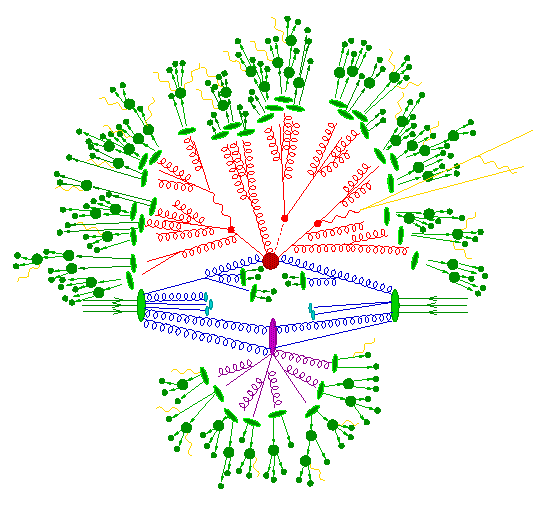
\includegraphics[width=0.90\textwidth]{Figures/LHC/HocheMCEG_final.pdf}
    \caption{This is a diagram of a simulated proton-proton collision. The hard collision is shown in the centre in red. In purple is the secondary hard scattering event. The parton shower is drawn in blue. Hadronisation is sketched in light green, and the subsequent hadron decays and final state particles are shown in dark green. Finally, the electromagnetic radiation is presented in yellow. This figure is from Reference~\cite{hoche2015introduction}.}
    \label{fig:MCEG}
\end{figure}

\subsubsection{Validation of V+jets production in Herwig7 with NLO multi-jet merging}
As part of the \ATLAS author qualification task, multi-leg merging at next-to leading order accuracy using the Matchbox framework in \herwig{7} was explored, with a focus on the vector boson plus jets process. Further details of the task and progression can be found on JIRA (\href{https://its.cern.ch/jira/browse/AGENE-1453}{\code{\textcolor{blue}{AGENE-1453}}}), and in the technical report of~\cite{Huang:2676143}.

\subsection{Monte Carlo samples}
\label{sec:montecarlopred}
This section provides a description of the event samples that are used for this analysis in the standard description of the ATLAS collaboration. These state-of-the-art predictions used to model the signal processes at detector-level and particle-level for this analysis, and to construct the response matrices that correct the data for detector effects. 
\subsection{\qqFourL}
The dominant \qqFourL process is simulated using the \SHERPA {2.2.2} event generator~\cite{Bothmann:2019yzt} with the \nnpdfnnlo{} set of PDFs~\cite{Ball:2014uwa}. The matrix elements are calculated at next-to-leading order accuracy for final states with zero and one jet, and at leading order accuracy for two- and three-jet final states. The different parton multiplicities are merged together and matched to the \SHERPA parton shower model based on the Catani-Seymour dipole factorization~\cite{Gleisberg:2008fv,Schumann:2007mg} using the MEPS@NLO prescription~\cite{Hoeche:2011fd,Catani:2001cc,Hoeche:2009r}. A dedicated set of tuned parton-shower parameters developed by the \SHERPA authors are used. 
An alternate sample of the \qqFourL process is generated using  \POWHEGBOX v2~\cite{Alioli:2010xd,Melia:2011tj,Nason:2013ydw}. The sample is generated at NLO accuracy and interfaced to \PYTHIA 8.186 for the simulation of the parton shower, hadronization, and underlying event. The tuning parameters are set according to the AZNLO tune~\cite{STDM-2012-23}. The sample is corrected to higher order effects using a k-factor obtained with \textsc{Matrix} NNLO QCD prediction~\cite{Cascioli:2014yka,Grazzini:2015hta,Grazzini:2017mhc,Kallweit:2018nyv}. The $K$-factor is defined as the ratio of the NNLO cross-section to the NLO cross-section and applied as a function of \mFourL{}. 
Virtual electroweak NLO effects are accounted for by reweighting both samples with a mass-dependent $K$-factor. The high-order real electroweak contribution of $ZZ$ plus two jets is modelled separately in a \SHERPA{} {2.2.2} sample. 

\subsection{\ggFourL{}}
The gluon-gluon initiated \ggFourL{} process is modelled by \SHERPA{} 2.2.2 at leading order QCD for up to one additional parton emission. The \SHERPA parton shower model based on the Catani-Seymour dipole factorisation is used. Also included in this sample is the s-channel Higgs signal \ggS{} and its interference with the SM box diagram, which has a sizeable contribution above \unit{130}{\GeV}. For particle-level masses below \unit{130}{\GeV} the sample includes on the \ggFourL box diagram because the role of interference is negligible. An NLO QCD $K$-factor is derived using the ratio of the \SHERPA{} sample to an MCFM NLO sample~\cite{Campbell:2011bn}. This is applied as a mass-dependent weight.
An additional constant $K$-factor of 1.2 is applied to account for NNLO effects on the off-shell Higgs production cross-section~\cite{Passarino:2013bha,deFlorian:2016spz}. The sample has a generator cut of $\mll > 10~\GeV$ for same-flavour, opposite-charge lepton pairs. The contribution is below this cut is accounted for through the reweighting to MCFM prediction. Scale and PDF uncertainties are derived in the same way as for the \SHERPA{} \qqFourL{} sample.

\subsection{On-shell Higgs}
The resonant Higgs-boson production is an important process and is generated independently using the most precise description available. The SM Higgs can be produced via gluon-gluon fusion, vector-boson fusion (VBF), Higgstrahlung ($VH$), and in association with a top quark pair ($t\overline{t}H$). The \texttt{PDF4LHC15nnlo} and \texttt{PDF4LHC15nlo} PDF set~\cite{Butterworth:2015oua} are used, alongside AZNLO tune for all on-shell Higgs samples. The dominant gluon–gluon fusion production channel is simulated using the \powheg{} NNLOPS program~\cite{Hamilton:2013fea, Hamilton:2015nsa,Alioli:2010xd,Nason:2004rx,Frixione:2007vw} at NNLO accuracy in QCD, and matched to \pythia~\cite{Sjostrand:2014zea} for the simulation of the parton shower and non-perturbative effects. The sample is normalized to N$^3$LO in QCD cross-sections, which has been calculated for the gluon-fusion process, and corrected for NLO electroweak effects~\cite{deFlorian:2016spz,Anastasiou:2016cez,Anastasiou:2015ema,Dulat:2018rbf,Harlander:2009mq,Harlander:2009bw,Harlander:2009my,Pak:2009dg,Actis:2008ug,Actis:2008ts,Bonetti:2018ukf}. 
\powheg~\cite{Nason:2009ai,Alioli:2010xd,Nason:2004rx,Frixione:2007vw} is interfaced to \pythia{} for the vector-boson fusion process, the $WH$ and $ZH$ production process, and the small contribution from associated productions with a $t\overline{t}$ pair. All are estimated with matrix elements up to NLO in QCD. For VBF, the prediction is reweighted to an approximate-NNLO QCD cross-section with NLO electroweak corrections~\cite{Ciccolini:2007jr,Ciccolini:2007ec,Bolzoni:2010xr}. For VH, the prediction is normalized to an NNLO QCD cross-section calculation with electroweak NLO corrections~\cite{Ciccolini:2003jy,Brein:2003wg,Brein:2011vx,Denner:2014cla,Brein:2012ne}. 
The uncertainties for the on-shell Higgs samples are identical of that of a previous Higgs analysis, the largest of which are from the QCD scale and PDF uncertainties. A detailed description can be found in Reference~\cite{HIGG-2016-22}. 
%  The simulation achieves NNLO accuracy for arbitrary inclusive $gg\to H$ observables by reweighting the Higgs boson rapidity spectrum in \texttt{Hj-MiNLO}~\cite{Hamilton:2012np,Campbell:2012am,Hamilton:2012rf} to that of HNNLO~\cite{Catani:2007vq}.

\subsection{$VVV$ and $t\overline{t}V(V)$}
A smaller contribution to the four-lepton final state originates from triboson processes, and vector-boson production in association of top-quark pairs. These are referred to as $VVV$ (for $WWZ, WZZ$ and $ZZZ$) and $t\overline{t}V(V)$ (for $t\overline{t}Z$ and $t\overline{t}WW$) respectively. The tribon processes are modelled with \SHERPA{} 2.2.2 at NLO accuracy in QCD, with a Catani–Seymour dipole factorization based parton shower provided by \SHERPA{}. Two samples are provided for the  $t\overline{t}V(V)$ contribution. The first is simulated with \SHERPA{} 2.2.0 at LO accuracy up to final states with one additional jet. This sample is used to construct the response matrix used to correct the data for detector effects. The second prediction is produced with the \madgraph~2.3.3~\cite{Alwall:2014hca} generator at NLO accuracy interfaced to \PYTHIAV{8.210}~\cite{Sjostrand:2014zea}. This particle-level predictions of this sample is used to compared against the data for the interpretations of Section \ref{sec:interpretations}. A flat uncertainty of $\pm15\%$ to account for the differences between the two samples is is assigned.

\subsection{Corrections}
All MC events are processed through GEANT4~\cite{Geant4} to simulate the expected response of the ATLAS detector. Next, the samples are passed through the same object reconstruction and identification algorithms as the data and the analysis selection is applied. Pile-up is simulated with \PYTHIAV{8.186} as inclusive inelastic $pp$ collisions. The events are then reweighted to reproduce the distribution of the mean number of interactions per brunch crossing (33.7 on average for the whole dataset). Lastly, events are  reweighted to account for the differences of the lepton reconstruction, identification, isolation, and vertex-matching efficiencies between data and simulation.


  \section{Background estimation}
\label{sec:background}

\subsection{Defining leptons}

The four lepton channel is quite the golden channel, as it has a very clean signature with minimal background. In fact, the single dominant background in this analysis is when one or more of the reconstructed leptons in the quadruplet are not real leptons; rather they are misidentified objects in the detector mimicking the same signature \cite{varnes2016poisson}. These "leptons" are non-prompt, and can be referred to as a fake lepton, whereas a lepton produced from the hard scatter is a prompt, real lepton. One source of fake leptons is from hadron decays. In the case of the electron, photon conversion and hadronic jets misidentified due to their large and narrow deposit in the electromagnetic calorimeter can also play a role. In this analysis, around three-quarters of the fakes originate from \Pbottom-hadron decays in \Z plus jets and \Ptop\APtop events. 

The size and behaviour of the fake lepton background - also referred to as the reducible background - are usually estimated using data-driven methods because they are not well modelled by simulation \cite{varnes2016poisson}. One such method is the Fake Factor method. This method depends on two sets of lepton criteria: a tight criteria that selects leptons which make it into the signal region, and a loose criteria that is similar but less restrictive. The leptons selected by the latter are referred to as baseline leptons, and the baseline leptons that additionally pass the tight criteria are the signal leptons. The rest of this section will also touch on baseline-not-signal leptons; these are leptons that pass the "baseline" loose selection, but do not make the "signal" tight selection. 

\subsection{Fake Factor method}

The Fake Factor method relies on the calculation of a fake efficiency, $f$, which is the fraction of fake baseline leptons pass the tight selection criteria and become signal leptons. Because fake leptons not well modelled in simulation, the fake efficiency is calculated in data, in an alternative region of phase space that is enriched with fake leptons. 

Using the Fake Factor $F$, the number of baseline leptons, and the number of real baseline leptons, the number of fake signal leptons can be calculated. Note that the FF method assumes good modelling in the real component of the simulation since $N^{\text{baseline}}_{\text{real}}$ is taken from MC.
$$N_{\text{fake}}^{\text{signal}} = F(N^{\text{baseline}}-N^{\text{baseline}}_{\text{real}})$$
%% Smoothing
Smoothing on the raw output of the reducible background estimate is performed. The raw output, due to low statistics in certain bins, have pronounced, jagged features that resemble resonances. Of course, resonant peaks should not exist. The smoothing procedure is therefore used to obtain a more even shape, minimizing the impact of any outlier bins that had a large Fake Factor weight. In order to smooth the distribution, an intermediate, finer binning is assigned to each observable and the background estimate is run. The fine-binned intermediate background distribution is smoothed with Friedman's super smoother. Lastly, the final background estimate is obtained by integrating over the smoothed distribution using the coarser, original binning. 

\subsection{Fake background uncertainties}
\label{ssec:fakeuncertainty}

In the fake-factor background estimate, there are five sources of uncertainty considered:
\begin{enumerate}
    \item Dominant in the low- and high-mass tails where \mFourL < 150 GeV and \mFourL > 350 GeV is the statistical uncertainty of the number of events with in the control region. This is propagated through the measurement via the bootstrap method.
    \item The dominant uncertainty in the mid-range region 150 < \mFourL < 350 GeV are the theory uncertainties associated with the subtraction of prompt-leptons in the control region. These come primarily from QCD scale variations in $WZ$ events. 
    \item A smaller contribution comes from the uncertainties in the Monte-Carlo predictions. This covers the modelling of prompt baseline-not-signal leptons, which get subtracted from the background estimation.  
    \item Fourth is the statistical uncertainty in the control region data used for the calculation of the fake factor. This contribution is subdominant. 
    \item Lastly there is a very small uncertainty from the arbitrary choice of number of intermediate bins used in the background smoothing procedure. It is accounted for by comparing the nominal prediction using 500 bins with alternate predictions using 250 or 1000 bins. 
\end{enumerate}

 \section{Detector-level results}
\label{sec:m4lrecoresults}
In this section the detector-level selected events are presented and compared to the SM predictions for the single $Z$, Higgs, \onshellZZ and \offshellZZ mass regions, and for the inclusive \mFourL{} distribution. The reducible background described in Section~\ref{sec:background} is also included. 

The number of selected events in the four \mFourL{} regions over the full fiducial phase space is presented in Table~\ref{tab:RecoYieldTablePerProcess}, along with the predicted number of events, and the predicted background contribution from non-prompt leptons. For the \qqFourL{} process the \SHERPA{} simulation is used. The combined uncertainties (systematic and statistical) are also quoted. The uncertainty in the total prediction takes into account correlations between processes, and therefore contributions in a given column do not trivially add up in quadrature to give the total. Uncertainties in the predictions arise from the sources discussed in Sections~\ref{sec:background} and~\ref{sec:uncertainties}. 

\begin{table}
    \centering    
  \begin{tabular} {l  c  c  c  c  c }
 \hline 
  & \multicolumn{5}{c}{Region} \\
      & Full   & \ZFourL{}  & \HFourL{}  & Off-shell $\Z\Z$  & On-shell $\Z\Z$   \\

 \hline 
\qqFourL{} & $6100 \pm 500$  & $1490 \pm 120$  & $128 \pm 10$  & $800 \pm 60$  & $3640 \pm 280$ \\
\ggFourL{} & $680 \pm 90$  & $10.8 \pm 2.9$  & ~~$3.9 \pm 0.7$  & $49 \pm 6$  & $620 \pm 80$ \\
\HFourL{}  & $245 \pm 20$  & ~~$2.16 \pm 0.18$  & $207 \pm 17$  & $33.5 \pm 3.1$  & $1.98 \pm 0.20$ \\
$VVV$  & $35 \pm 4$  & ~~$0.018 \pm 0.005$  & ~~$0.127 \pm 0.018$  & ~~$2.05 \pm 0.22$  & $32.9 \pm 3.4$ \\
$t\bar{t}$\V(\V) & $123 \pm 19$  & ~~$1.37 \pm 0.22$  & ~~$1.2 \pm 0.2$  & $15.5 \pm 2.4$  & $105 \pm 16$ \\
Background & $330 \pm 50$  & $44 \pm 8$  & $26 \pm 5$  & $129 \pm 19$  & $139 \pm 30$ \\    
\hline 
Total Pred. & $7500 \pm 500$  & $1540 \pm 110$  & $367 \pm 19$  & $1030 \pm 60$~~  & $4530 \pm 290$ \\
\hline 
Data & $7755 $  & $1452 $  & $379 $  & $1095 $  & $4828 $ \\
 \hline 
 \end{tabular}
     \caption{Predicted reconstruction-level yields per process and in total,
      compared with observed data counts, over the full fiducial phase space and in the
      following regions of
      $\mFourL$: \ZFourL{}  ($60 < \mFourL < 100$~\GeV), \HFourL{}  ($120 <
\mFourL < 130$~\GeV), off-shell $\Z\Z$  ($20 <
\mFourL < 60$~\GeV\ or $100 <
\mFourL < 120$~\GeV\ or $130 <
\mFourL < 180$~\GeV) and  on-shell $\Z\Z$ ($180 <
\mFourL < 2000$~\GeV).
     The background row is events with non-prompt leptons,
     including those from $\Z{} + \Upsilon{}$ events.
      The \HFourL{} row includes only the
      on-shell Higgs boson contribution, with off-shell contributions included in
     \ggFourL{}. This table is from Reference~\cite{m4l_internalnote}. \label{tab:RecoYieldTablePerProcess} }
\end{table}

Figure~\ref{fig:recoresults1} shows the inclusive \mFourL{} distribution at the detector level. The data are plotted in black along with the uncertainties. The SM prediction is separated into the individual dominant processes described in Section~\ref{sec:fourlepmotivation} and plotted as stacked histograms. 
Overall the data are in good agreement with the predictions, with some minor fluctuations in the high mass bins due to low statistics. The detector-level plots for the rest of the observables are not shown in the scope of this thesis, but are published in Reference~\cite{m4l2021_paper}. 
\begin{figure}[htb]
\centering
 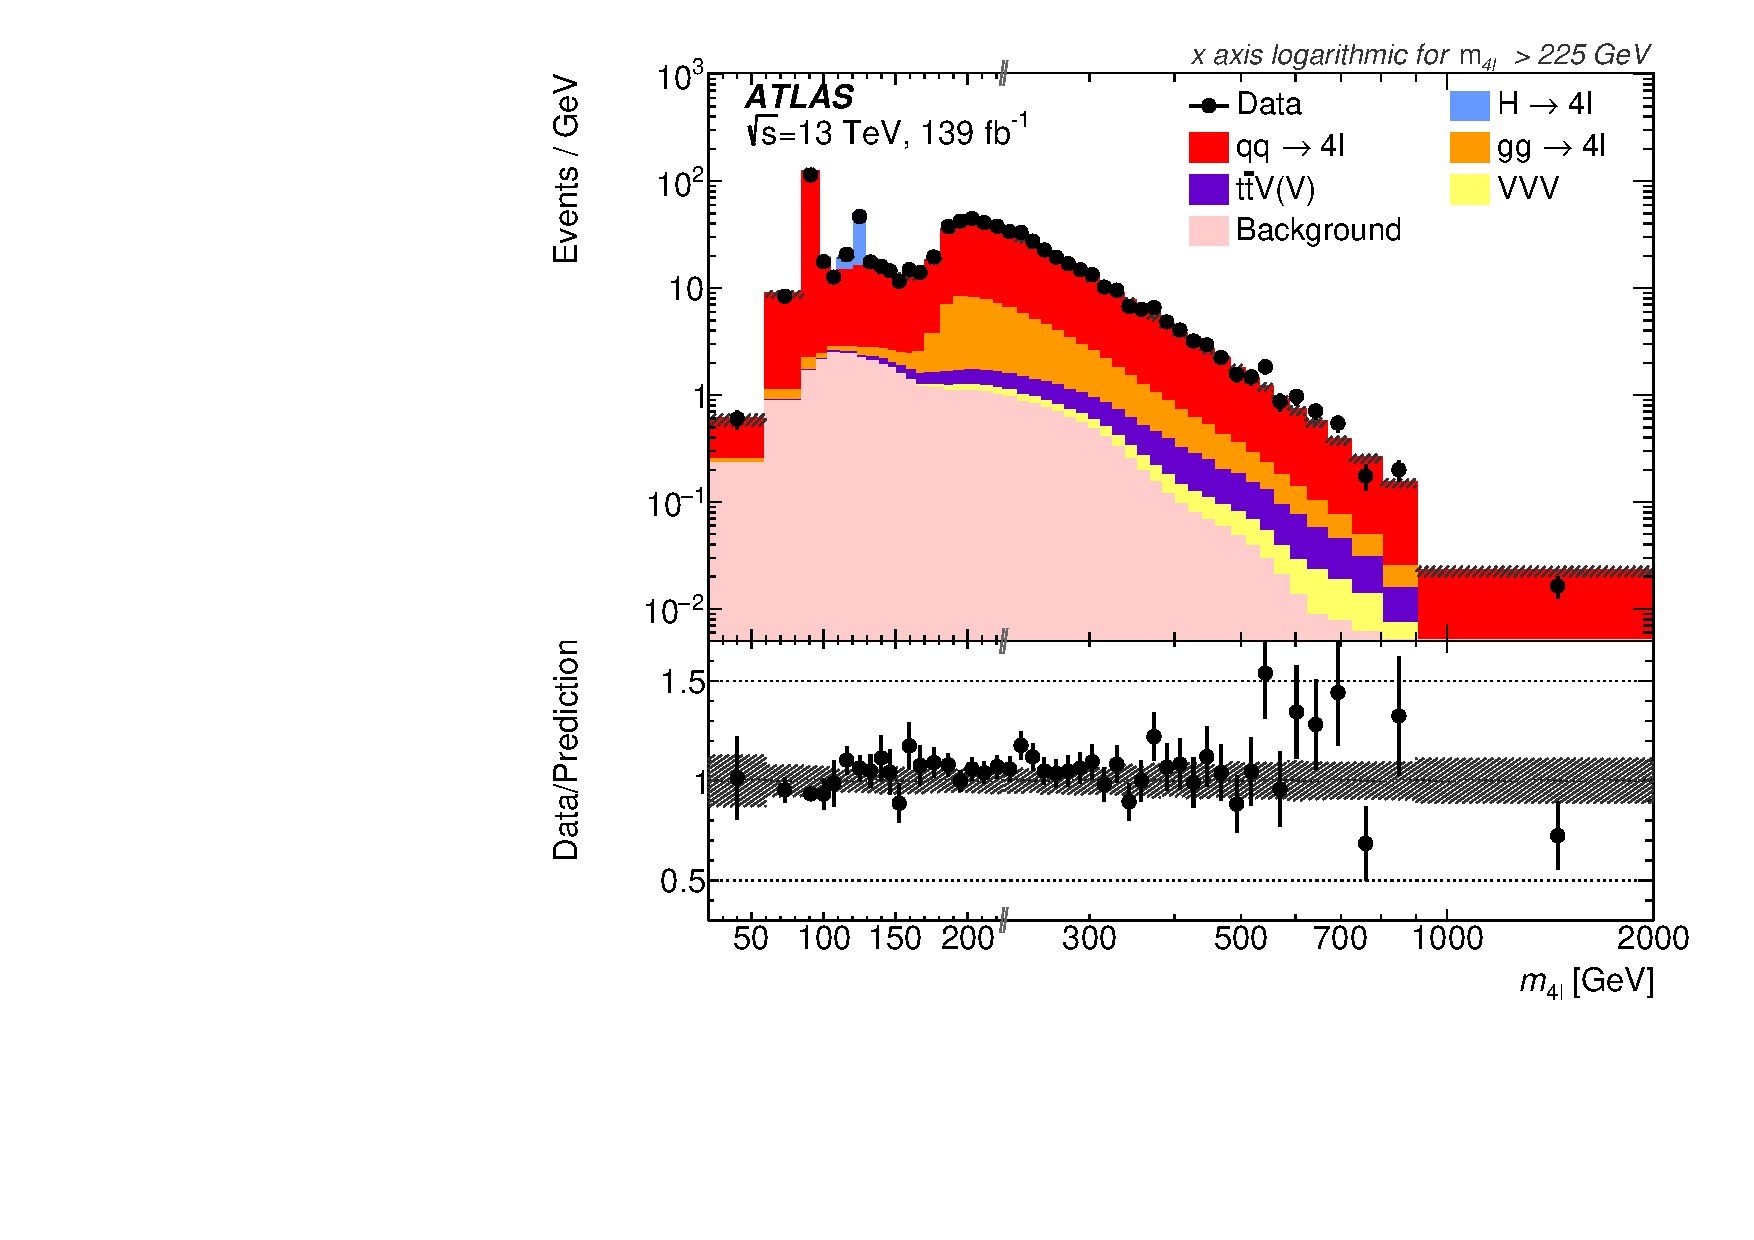
\includegraphics[width = 0.7\textwidth]{Figures/m4l/Overlay_M4l_0__forPaper.pdf}
    \caption{Observed reconstruction-level \mFourL{} distribution compared with the SM prediction, using
      \SHERPA{} for the \qqFourL{} simulation.
     The statistical uncertainty of the
      data is displayed as error bars and systematic uncertainties
      in the prediction are shown as a grey hashed band.  The
      ratio of the data to the prediction is shown in the lower
      panel.  The $x$-axis is on a linear scale until $\mFourL = 225$~\GeV,
where it switches to a logarithmic scale, as indicated by the double
dashes on the axis.
      There is one additional data event reconstructed with 
$\mFourL = 2.14$~\TeV, while 0.4 events are expected from simulation for
$\mFourL > 2$~\TeV. This figure is from Ref.~\cite{m4l2021_paper}. \label{fig:recoresults1}}
\end{figure}

  %% Unfolding and respective studies
\section{Correcting for detector effects}
\label{sec:unfolding}

When an observable is measured by a particle physics experiment, it is important to note that the measured distribution, (i.e. what the particle detector sees) is not what truly occurs at the particle-level. Rather, it is a convolution of the underlying physics process with the effects of the detector. The \ATLAS detector, although an astonishing feat of technology, is still subject to resolution, acceptance, and efficiency limitations. The data at the detector level is smeared and includes the effects of these limitations. For an inclusive measurement such as the four-lepton invariant mass distribution, it is often desirable to correct for these detector effects and present the data at the particle-level. In doing so, the measurement may be directly compared to theoretical predictions, as well as particle-level results from other experiments, in the years to come. In high energy physics, the term coined for this correction procedure is unfolding.

When Unfolding Makes Sense
4
1. Results from experiment A and B with different response function are to be
compared
2. It is too complicated to publish the response function of the detector along
with the data
Detector response might be very complex, e.g., time dependent
Sometimes computer code reflecting the response would have to be published
Danger that future users don't use the filter correctly

\subsection{Unfolding methodology}
\label{subsec:unfmethod}

Unfolding in particle physics can be more generally referred to as a deconvolution. The generic problem statement of deconvolution is to derive a relationship between the true distribution $T(x)$ and the recorded distribution $D(y)$. The two are related by a smearing function $R(x,y)$, which encompasses the instrumentation effects in making the measurement. 
\begin{equation} \label{eq:unfintegral}
    T(x)=\int S(x,y)D(y)dy
\end{equation}
Due to the discretised nature of histograms, the unfolding problem can be stated as a matrix equation:
\begin{equation} \label{eq:unfmatrix}
    x_i=S_{ij}y_j
\end{equation}
where $R$ represents the a smearing matrix of sorts, \todo{add more}$T$ is the true histogram at particle-level, and $D$ is the reconstructed histogram at detector-level. 

For the four-lepton invariant mass analysis, an iterative unfolding method motivated by Bayesian statistics, popularised by Giulio D’Agostini, is chosen. The method iteratively applies the three inputs described above to the measured distributions while using the particle-level SM prediction as a prior.

\subsubsection{An iterative Bayesian approach to unfolding}
\label{ssec:bayesianunfolding}
Let there be a set of causes $C_i$, that can produce one effect $E$. 
\begin{equation}
    P(C_i|E)=\dfrac{P(E|C_i)\cdot P(C_i)}{\Sigma_{k=1}P(E|C_k)\cdot P(C_k)}
\end{equation}

\begin{itemize}
    \item $P(C_i|E)$: given the effect, ithe conditional probability that it was produced from the $i$-th cause.
    \item $P(E|C_i)$: for the $i$-th cause, the conditional probability that the effect is produced.
    \item $P(C_i)$ is the initial probability of the $i$-th cause.
\end{itemize}
If there are multiple possible effects for the causes, then the formula can be generalized to be:
\begin{equation}
    P(C_i|E_j)=\dfrac{P(E_j|C_i)\cdot P(C_i)}{\sum_{k=1}P(E_j|C_k)\cdot P(C_k)}
\end{equation}
The number of expected events for each cause $C_i$ can be obtained by multiplying the number of observations made for effect $j$ with the probability it had been due to cause $i$, and summing over all effects:
\begin{equation} \label{eq:numcause}
    N(C_i)=\sum_jN(E_j)\cdot P(C_i|E_j).
\end{equation}
Here a parallel can be drawn back to equation \ref{eq:unfmatrix}, where $N(C)={N(C_1),N(C_2),...,N(C_n)}$ represents the number of events in the $n$ bins of the true histogram $x_i$, and $P(C_i|E_j)$ corresponds to $R$. Combining these equations, the procedure for estimating the true histogram can be written as:
\begin{equation}
    x_i=\sum_{j=1}^n\dfrac{R_{ij}\cdot P(x_i)}{\sum_{k=1}^nR_{kj}\cdot P(x_k)}y_j.
\end{equation}
Here the matrix defined as $R_{ij}$ is the response matrix. The denominator in the equation is a normalisation factor using the y-projection of the matrix. $P(x_i)$ is the prior, which is updated in each iteration with the unfolded true distribution $x_i$, also known as the posterior.
\todo[inline]{Perhaps mention other unfolding methods and justify choice of this one?}

\subsubsection{Unfolding inputs}

In this analysis the variables of interest are presented as histograms with a finite number of bins. In order to bring these distributions from reconstruction-level to particle-level, there are a number of correction factors to consider:

\begin{itemize}
    \item Fiducial fraction: this is a one-dimensional correction that accounts for events which do not enter into the fiducial region, but pass the detector-level selection nonetheless. These occur due to the finite resolution in the measurement the variables used to select events. The fiducial fraction is defined as the ratio of events that pass both fiducial and detector-level selection to events that pass detector-level selection only.
    \item Reconstruction efficiency: this accounts for the acceptance and efficiency of the detector in reconstructing an event. Of all the events that pass the fiducial selection, only a fraction will be successfully reconstructed and visible to the detector. Formally the reconstruction efficiency is also a one-dimensional correction; defined as the ratio of events which pass both the fiducial and detector-level selection to events that pass fiducial-level selection only.
    \item Migration matrix: each bin in the histogram of the measured observable represents a sub-range of observable values. Sometimes the detector may smear the observable's value high or low enough such that it gets filled to different bins in particle-level and detector-level. These are referred to as bin-to-bin migrations, and is corrected for by the migration matrix. This is constructed as a two-dimensional matrix using events which pass both fiducial and detector-level selection, with the value at particle-level on one axis and the value at detector-level on the other. The matrix, $M_{ij}$, represents the probability that an event which falls into bin $i$ at particle level will fall into bin $j$ when reconstructed at the detector-level. 
\end{itemize}

\subsubsection{Number of Bayesian iterations}

When using the iterative Bayesian method to unfold, the number iterations performed is a key parameter and must be optimised. The method, which uses the nominal MC distribution as an initial prior, results in a bias towards the original shape of the nominal prediction. A way to minimise this effect is to use the obtained unfolded distribution from the previous iteration as the prior for the subsequent unfolding iteration. The more iterations there are, the less dependence there is on the prior, and therefore the smaller the bias. A side effect, however, is that increasing the number of iterations also increases the statistical uncertainty. Fluctuations caused by limited statistics become amplified by the feedback in the algorithm. These effects are thoroughly studied in order to strike a balance between minimising the bias at the cost of increasing the statistical uncertainties.

One thousand toy distributions are generated using the detector-level Standard Model prediction where the value of each bin is randomly drawn from a Gaussian distribution. Each toy is unfolded following the procedure outlined in section \ref{ssec:bayesianunfolding}, where the nominal SM predictions are used to construct the response matrix and for the prior. The bias, written as
\begin{equation} \label{eq:unfbias}
    \text{Bias}_i=\dfrac{\sum_{j=1}^nM_{ij}\cdot x_j-y_i\cdot f_i}{y_i\cdot f_i},
\end{equation}
measures the difference between the product of the migration matrix and the unfolding output, and the product of the detector-level toy and the fiducial fraction. It is an assessment of the strength of the pull that the shape of the SM prior has on the unfolded toy result \todo{Read more about regularisation}. Additional, a statistical uncertainty from the unfolding procedure for each individual toy in each bin is quoted. Next, the bias significance\change[]{italics?} per bin is defined as the quotient of the bias and the statistical uncertainty. After sampling over all toys, the root-mean-square of the bias significance in each bin is calculated. Through the rms bias significance, the size of the bias in comparison to that of the statistical uncertainty is quantified and used as a criterion in determining the number of iterations. The requirement is to use the minimum the number of iterations needed for a bias significant lower than 0.5.

\missingfigure{Optimisation of number of unfolding iterations}

Figure \ref{fig:unfopt} shows the bias, the statistical uncertainty, and the rms bias significance for the inclusive \mFourL distribution. Here the minimum number of iterations for which the criterion is met is three. For the majority of the other measured distributions, three iterations of the unfolding are also found to be optimal. Two iterations are found to be sufficient for the following observables: \mZOne-\mFourL, \dPhill-\mFourL, and \dYPairs-\mFourL.

\subsection{Binning optimisation}
\label{subsec:binningopt}

The binnings of the measured distributions were optimised based on two factors: the number of events and the purity of each bin. Here the purity refers to the diagonal of the migration matrix normalised along truth, thus representing the fraction of truth events that end up in the same reconstructed event bin. There were a few iterations of the binning that were run with varying criteria, summarised in table \ref{tab:BinningVersions}.

The first iteration of the binnings were run with the nominal criteria. Here, depending on the number of events in the bin, the purity requirement varies. Bins with lower statistics have a high purity requirement to reduce bin-to-bin migrations. The minimum number of events required for each bin is 14. Between 14 and 20 events, the purity was required to be at least 80\%. Between 20 and 25 events the purity must be 70\% or higher. Finally for the higher statistics bins with more than 25 events the purity cut was 60\%. 

The binning algorithm is as follows. For the full \mFourL differential mass distribution from \unit{20}{\Gev} - \unit{2000}{\GeV}, the distribution was first split into very fine steps of \unit{1}{\GeV} bins from \unit{20}{\Gev}-\unit{450}{\GeV}. From \unit{450}{\Gev}-\unit{2000}{\GeV} wider steps of \unit{5}{\GeV} bins were used. Due to the fine nature of the bin widths, this initial binning failed to meet any of the binning criteria. Next, the binning algorithm starts from the low mass end and starts to merge adjacent bins together if the criteria were not met. For example, if bin number 1 [20,21] has > 10 events, the algorithm merges bin number 1 with the next bin. The new bin number 1 is now [20,22]. Once again, if this bin has > 10 events, it will merge again and become [20,23], and so on and so forth until 10 events has been reached. Of course the purity must also pass the required percentage for the number of events in the bin, otherwise further bin merging occurs.  

Next we have the \mFourL distributions in double differential slices of \ptFourL, \yFourL, and flavour channel. For these distributions, the fine binning was defined as the the binning of the full \mFourL differential mass distribution, i.e. the output of the algorithm described in the previous paragraph. Bins were once again checked for number events and purity, and merged as needed. This was implemented so that all \mFourL in each of the  \ptFourL, \yFourL, and flavour slices would have bin edges that match with the inclusive distribution. 

For the distributions measured double differentially in the four \mFourL regions corresponding to \Z, \Higgs, On-shell \ZZ, and Off-shell \ZZ, the same procedure was followed for binning optimisation. Each distribution had a fine binning defined, and the bins were merged from left to right of the x-axis until the criteria were met. 

\begin{table}[bp]
  \begin{tabular}{lllll}
                & Nominal              & High statistics             \\
    \midrule
                                & 14 (purity > 0.8) &   \\
     Minimum number of events & 20 (purity > 0.7) & 100    \\
                                &25 (purity > 0.6) &    \\
  \end{tabular}
  \caption{Three different versions of binning with varying criteria.}
  \label{tab:BinningVersions}
\end{table}

\subsection{Pre-unfolding weights}
\label{subsec:preuf}

When correcting the data for detector effects, one of the things to take into account is the efficiency correction. Recall from section \ref{subsec:unfmethod} that the efficiency correction is the fraction of reconstructed events that also pass the fiducial selection cuts. A significant contribution to this is the efficiency correction is efficiency in identifying, reconstructing, isolating, and track-to-vertex-association of (TTVA) leptons. These are dependent on lepton kinematics and calculated from Monte Carlo simulation, therefore they may not be accurate if the data differs from the prediction. To correct for this effect, the lepton efficiencies are measured as a function of the lepton transverse momentum (\pt) and pseudorapidity ($\eta$), and the inverse of this is applied as a per-lepton weight in the data. The term coined for this weight is the pre-unfolding weight, and as the name suggests it is applied prior to the unfolding procedure detailed in \ref{subsec:unfmethod}. 

\begin{figure}
    \begin{subfigure}{.49\textwidth}\centering
        \includegraphics[.99\textwidth]{Figures/m4l/UnfoldingStudies}
    \end{subfigure}
    \caption{Caption}
    \label{fig:my_label}
\end{figure}

Figure \ref{fig:preUF} shows the detector yield from simulation with and without the application of the pre-unfolding weights, compared to the particle yield. It is readily apparent that the detector yield comes much closer to the particle yield when pre-unfolding weights are applied. In some cases, the detector yield surpasses the particle yield around the resonance peaks. This is attributed to bin migrations, and has negligible effects on the final unfolded result. Also shown is the efficiency correction with and without the pre-unfolding weights. In general, a significant increase in efficiency throughout the whole \mFourL spectrum, ranging from 10\% at low mass, up to 25\% at high mass. The conclusion drawn from these plots is that a large portion of the event inefficiency can be accounted for using per-lepton corrections, bringing the reconstructed and particle level yield closer to one another, and minimising the correction needed when unfolding.

\subsection{Unfolding iterations optimization}
\label{ssec:unfoldingiterations}
With the observable binnings defined and the pre-unfolding weights applied, the next step is to optimize the number of iterations used in the unfolding. As described in Section \ref{ssec:bayesianunfolding}, the iterative Bayesian approach to unfolding uses the Standard Model prediction as an initial prior and therefore has a dependence on it. Fewer numbers of iterations therefore correspond to a larger regularizaton bias on the unfolded result. Contrarily, increasing the number of iterations reduces the bias at the cost of a larger statistical uncertainty and results that are more prone to large bin-to-bin fluctuations. The rest of this section describes the metric used to balance these effects and converge on an optimal number of iterations.

First, one thousand toy distributions are generated from the Standard Model predicted yield at the detector level by drawing random Gaussian distributed values for each bin. Under the assumption that the SM accurately describes the underlying physics, each toy distribution represents a possible observation. The toy distributions are unfolded using the nominal unfolding method (Section \ref{subsec:unfmethod}). The bias of the unfolded toy result is defined using the migration matrix $M$, the unfolded yield of the toy $U_{j}$ , detector-level yield of the toy $R_i$, and the fiducial fraction $f_i$ as:
\begin{equation*}
  \text{Bias}_{\text{reco bin }i} = \frac{\sum\limits_{\text{truth bin }j} M_{ij} \times U_{j} - R_{i} \times f_{i} }{R_{i} \times f_{i}},
\end{equation*}
The bias significance of the toy is then be calculated in each bin as the ratio of the bias and the estimated statistical uncertainty of the unfolding procedure. This ratio is a comparison of the sizes of the two effects. 

Next, the bias significance of the one thousand toys are combined into a singular root-mean-square value in each bin. As a result, a metric indicating how significant the bias is expected to be across a range of toy datasets assuming an underlying SM physics is created. The number of iterations is chosen to be the smallest possible while maintaining a root-mean-square bias significance of 0.5 or below. This choice corresponds to a factor two suppresion of the bias compared to the statistical uncertainty. For the majority of distributions, three iterations of the unfolding comfortably satisfy this criteria, whilst for \mZOne-\mFourL, \dPhill-\mFourL and \dYPairs-\mFourL two iterations is sufficient. 
% The bias defined in this way is a measure of to which degree the individual toy is pulled towards the original standard model shape by the regularisation procedure in the unfolding. 
\subsection{Closure tests}
\label{ssec:closuretests}
\subsubsection{Monte Carlo closure tests}

As detailed in Section \ref{subsec:unfmethod}, the unfolding procedure uses a response matrix that has been derived from Standard Model Monte Carlo predictions. A simple test that can be performed to check the validity of the unfolding method is to use the same SM MC prediction at reconstruction level as pseudo-data, unfold it, and compare it to the truth level prediction. This is a self-consistency check, and should yield the trivial result that the unfolded pseudo-data be identical to the truth distribution. This is the full MC closure test, and acts as a sanity check for the unfolding procedure. The test is shown in Figure \ref{fig:fullMCclosure} for the inclusive \mFourL distribution. Full closure is achieved as the unfolded distribution and the particle-level distribution are identical. This is the case for all other distributions as well.

Another similar validation, the half MC closure test, is also performed. This time, the SM samples are divided in two sets A and B based on whether their tagged event number is odd or even. Set A is used to construct the fiducial fraction, reconstruction efficiency, and migration matrix, while set B is used as pseudo-data and unfolded with the inputs from the set A. The unfolded distribution of the set B is then compared to the true distribution of the set B. The statistical uncertainties on both sub-samples are evaluated via the bootstrap method \cite{ATLAS_Bootsrap_2021}. Figure \ref{fig:halfMCclosure} shows the test result for the inclusive \mFourL spectrum. For this and all other distributions, closure is generally achieved within the statistical uncertainties in each bin, with no significant discrepancies. 

\begin{figure}
    \begin{subfigure}{.88\textwidth}\centering
        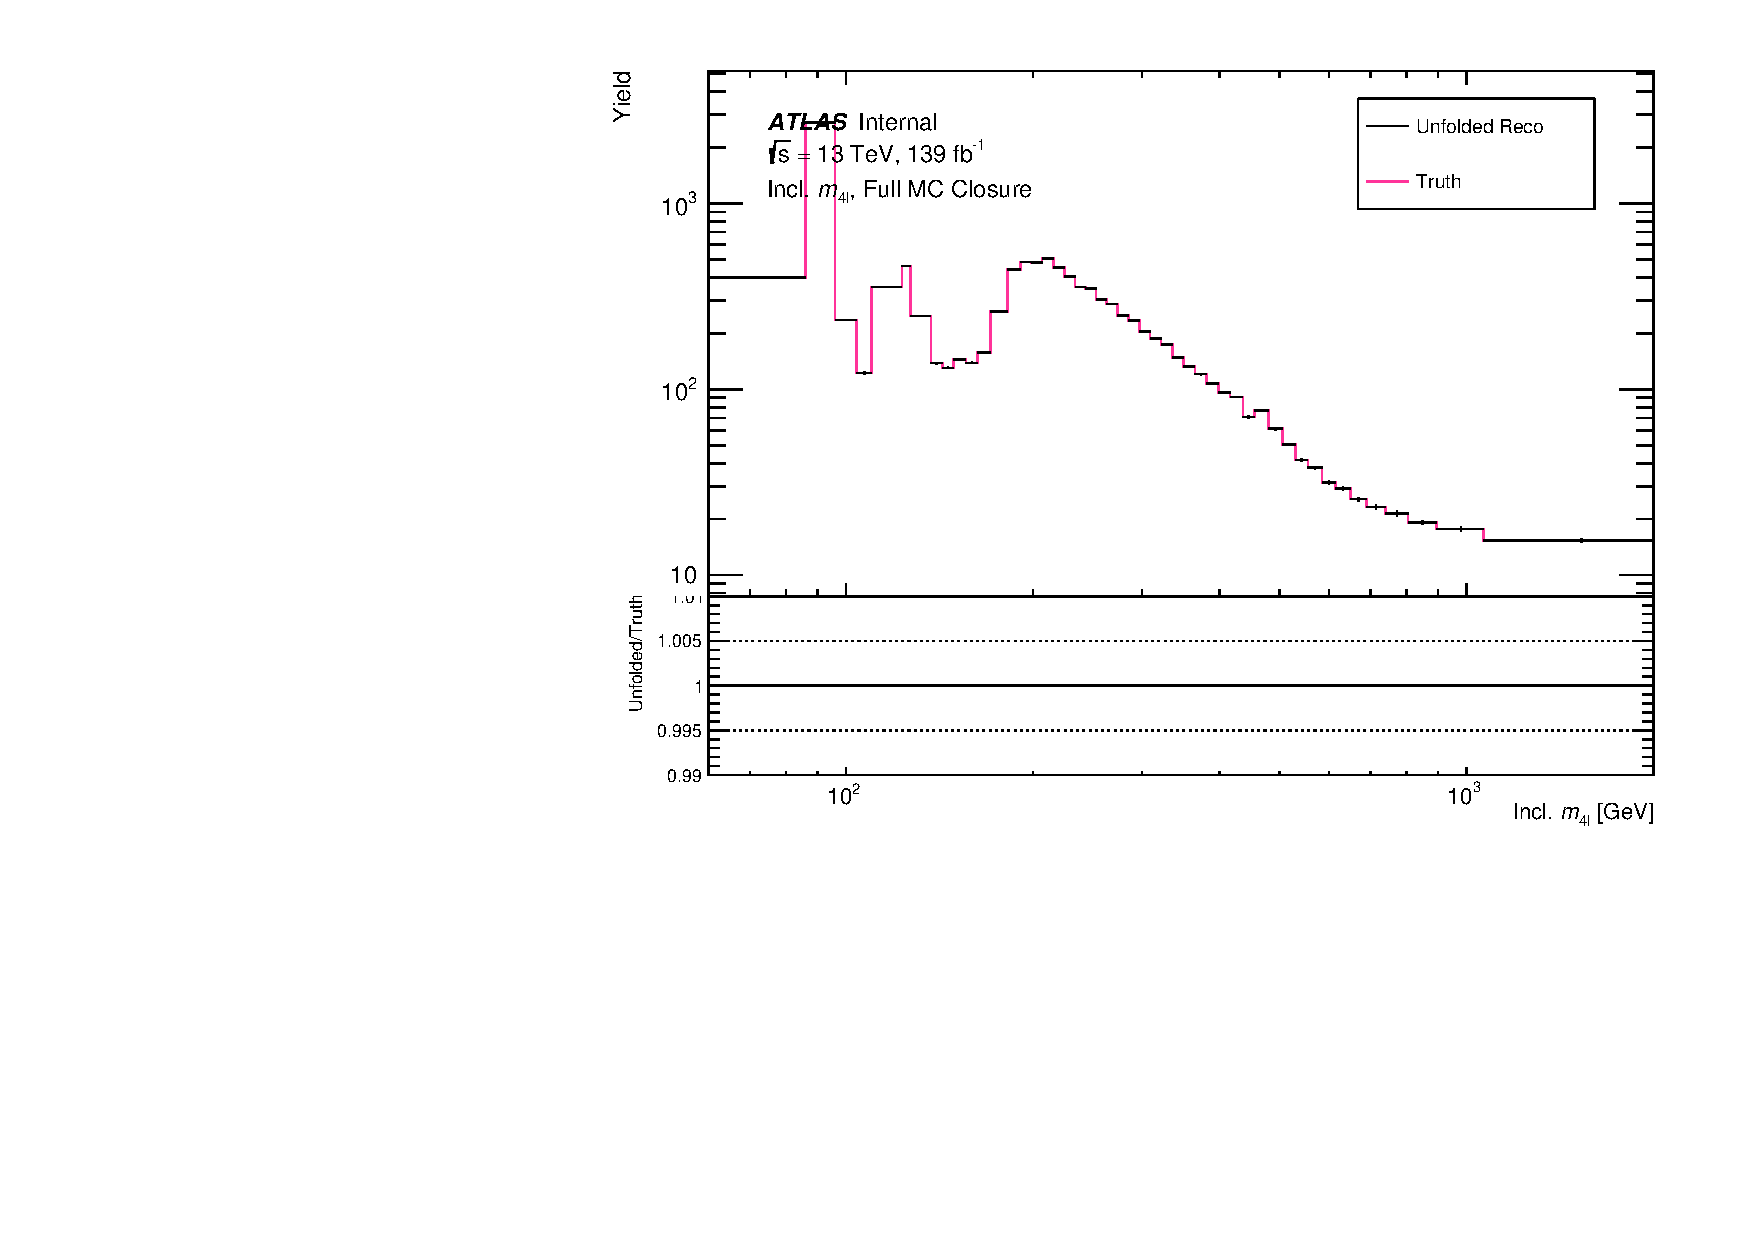
\includegraphics[width=0.90\linewidth]{Figures/m4l/MCClosure/FullMCClosure_inclm4l.pdf}\caption{}\label{fig:fullMCclosure}
    \end{subfigure}
        \begin{subfigure}{.8\textwidth}\centering
        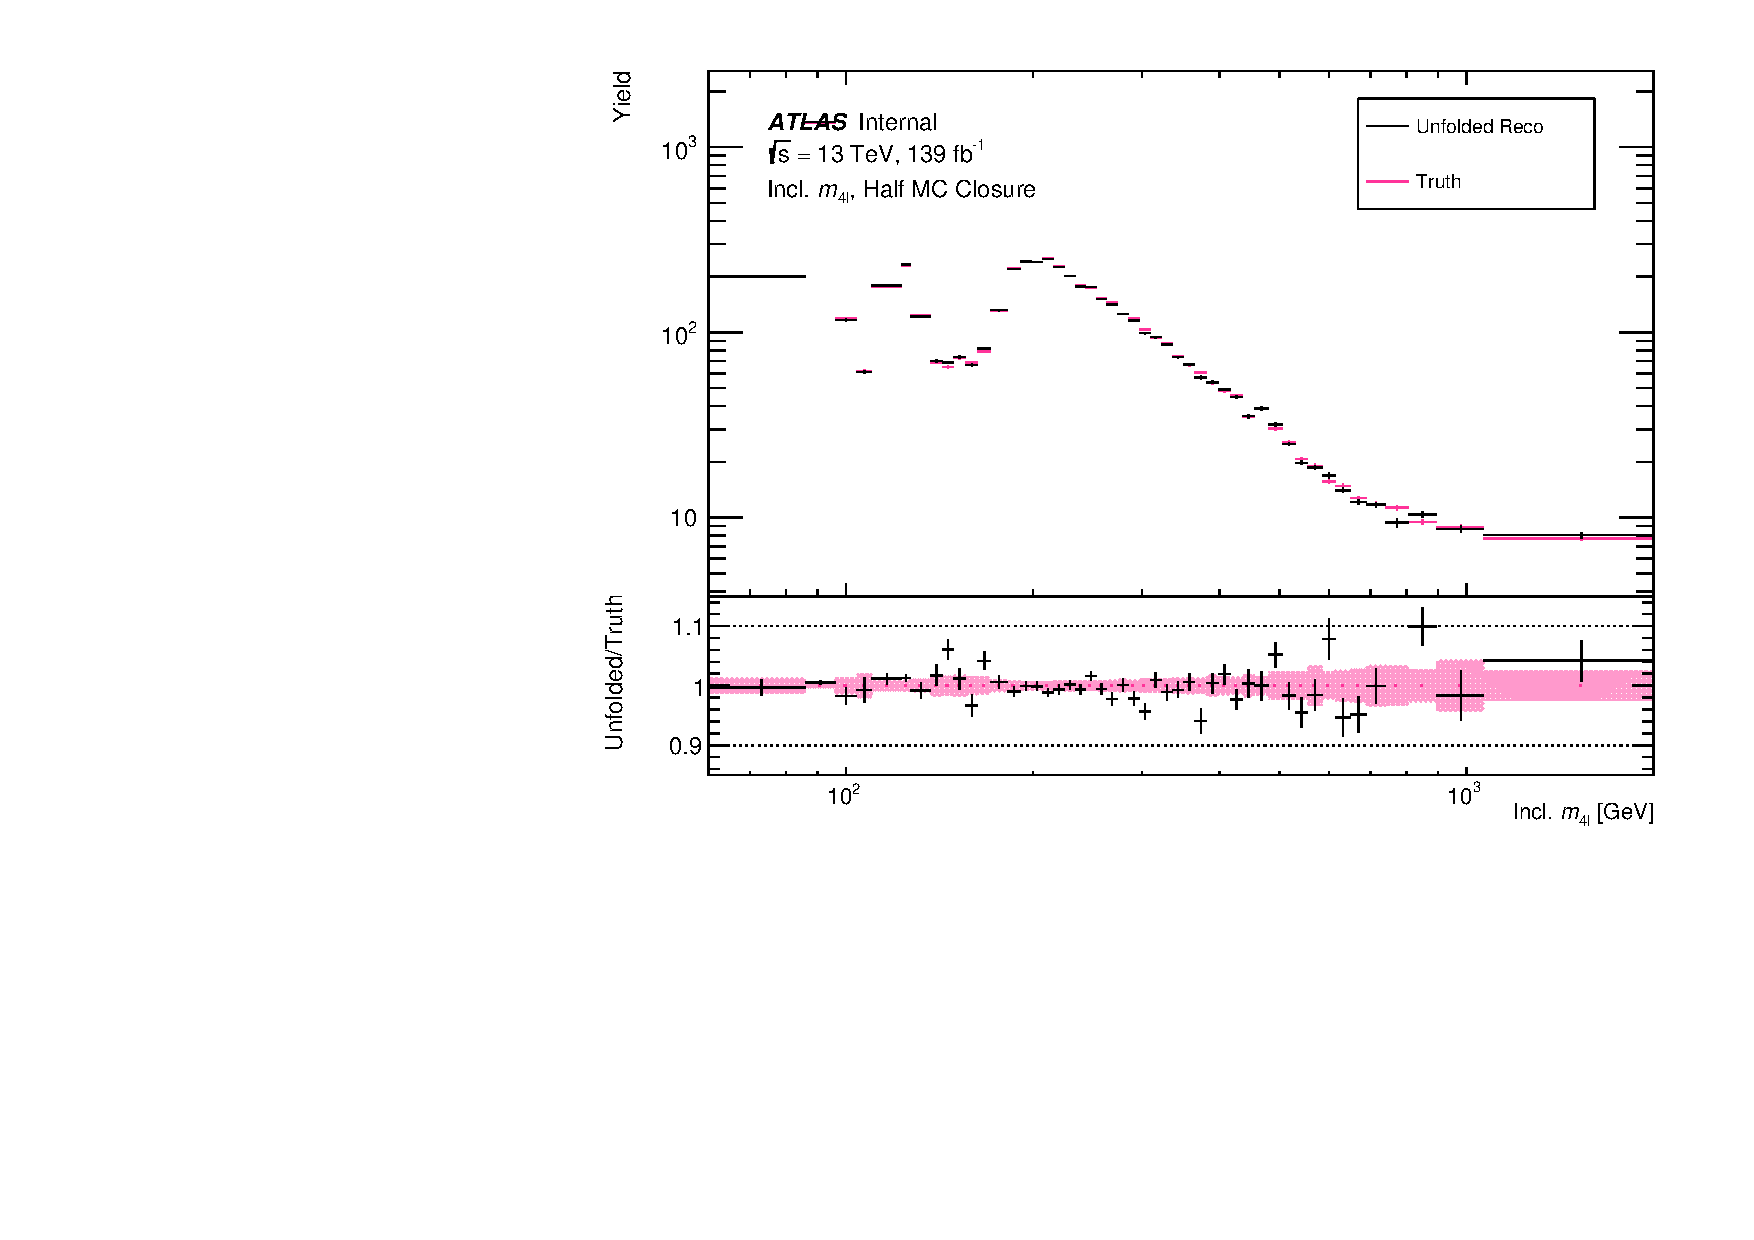
\includegraphics[width=0.99\linewidth]{Figures/m4l/MCClosure/HalfMCClosure_inclm4l.pdf}\caption{}\label{fig:halfMCclosure}
    \end{subfigure}
    \caption{Caption}
    \label{fig:MCclosure}
\end{figure}

\subsubsection{Data-driven closure tests}
\label{sssec:datadrivenclosure}
In order to assess the potential bias in the unfolding method, a data-driven closure test is performed separately for each measured distribution. For this test, a reweighting is conducted on the particle-level MC prediction such that the detector-level prediction represents more accurately the data. The function used for the reweighting is a smoothed function of the data to MC ratio. The reweighted prediction is used as pseudo-data and propagated through the nominal unfolding procedure. The difference between the reweighted particle-level prediction and the unfolded result in each bin is taken to be the systematic uncertainty of the unfolding method. A pictorial description of the process is given in Figure \ref{fig:m4ldatadriven} for the inclusive \mFourL spectrum. The associated systematic uncertainty is below 0.3\% across the full mass range. For the double differential observables, the derived systematic uncertainties averaging much less than 1\% but reaching 3\% in a few bins. Overall, it remains subdominant compared to other sources of uncertainty.
\begin{figure}[htb!]
    \begin{subfigure}{.49\textwidth}\centering
      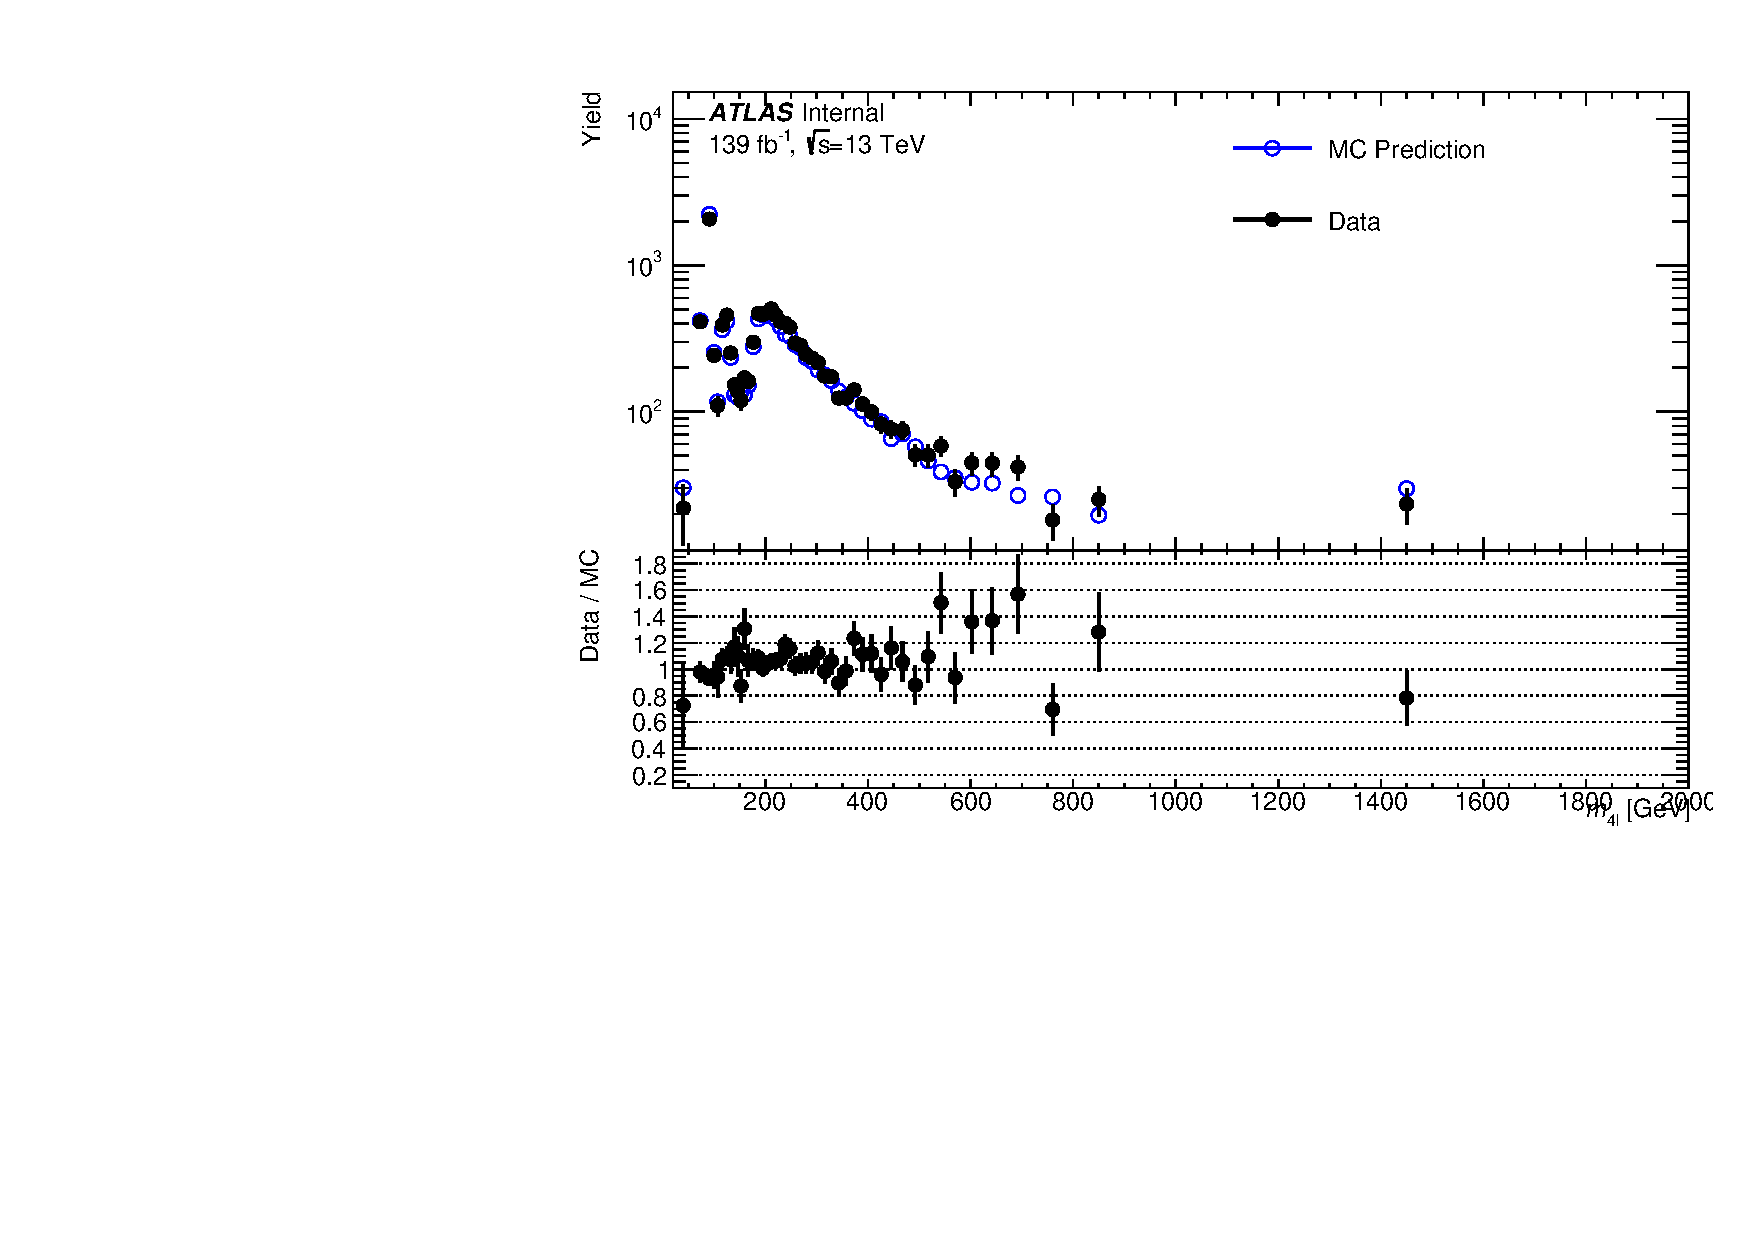
\includegraphics[width=.99\linewidth]{Figures/m4l/DataDriven/RatioM4l.pdf}\caption{}
    \end{subfigure}
    \begin{subfigure}{.49\textwidth}\centering
      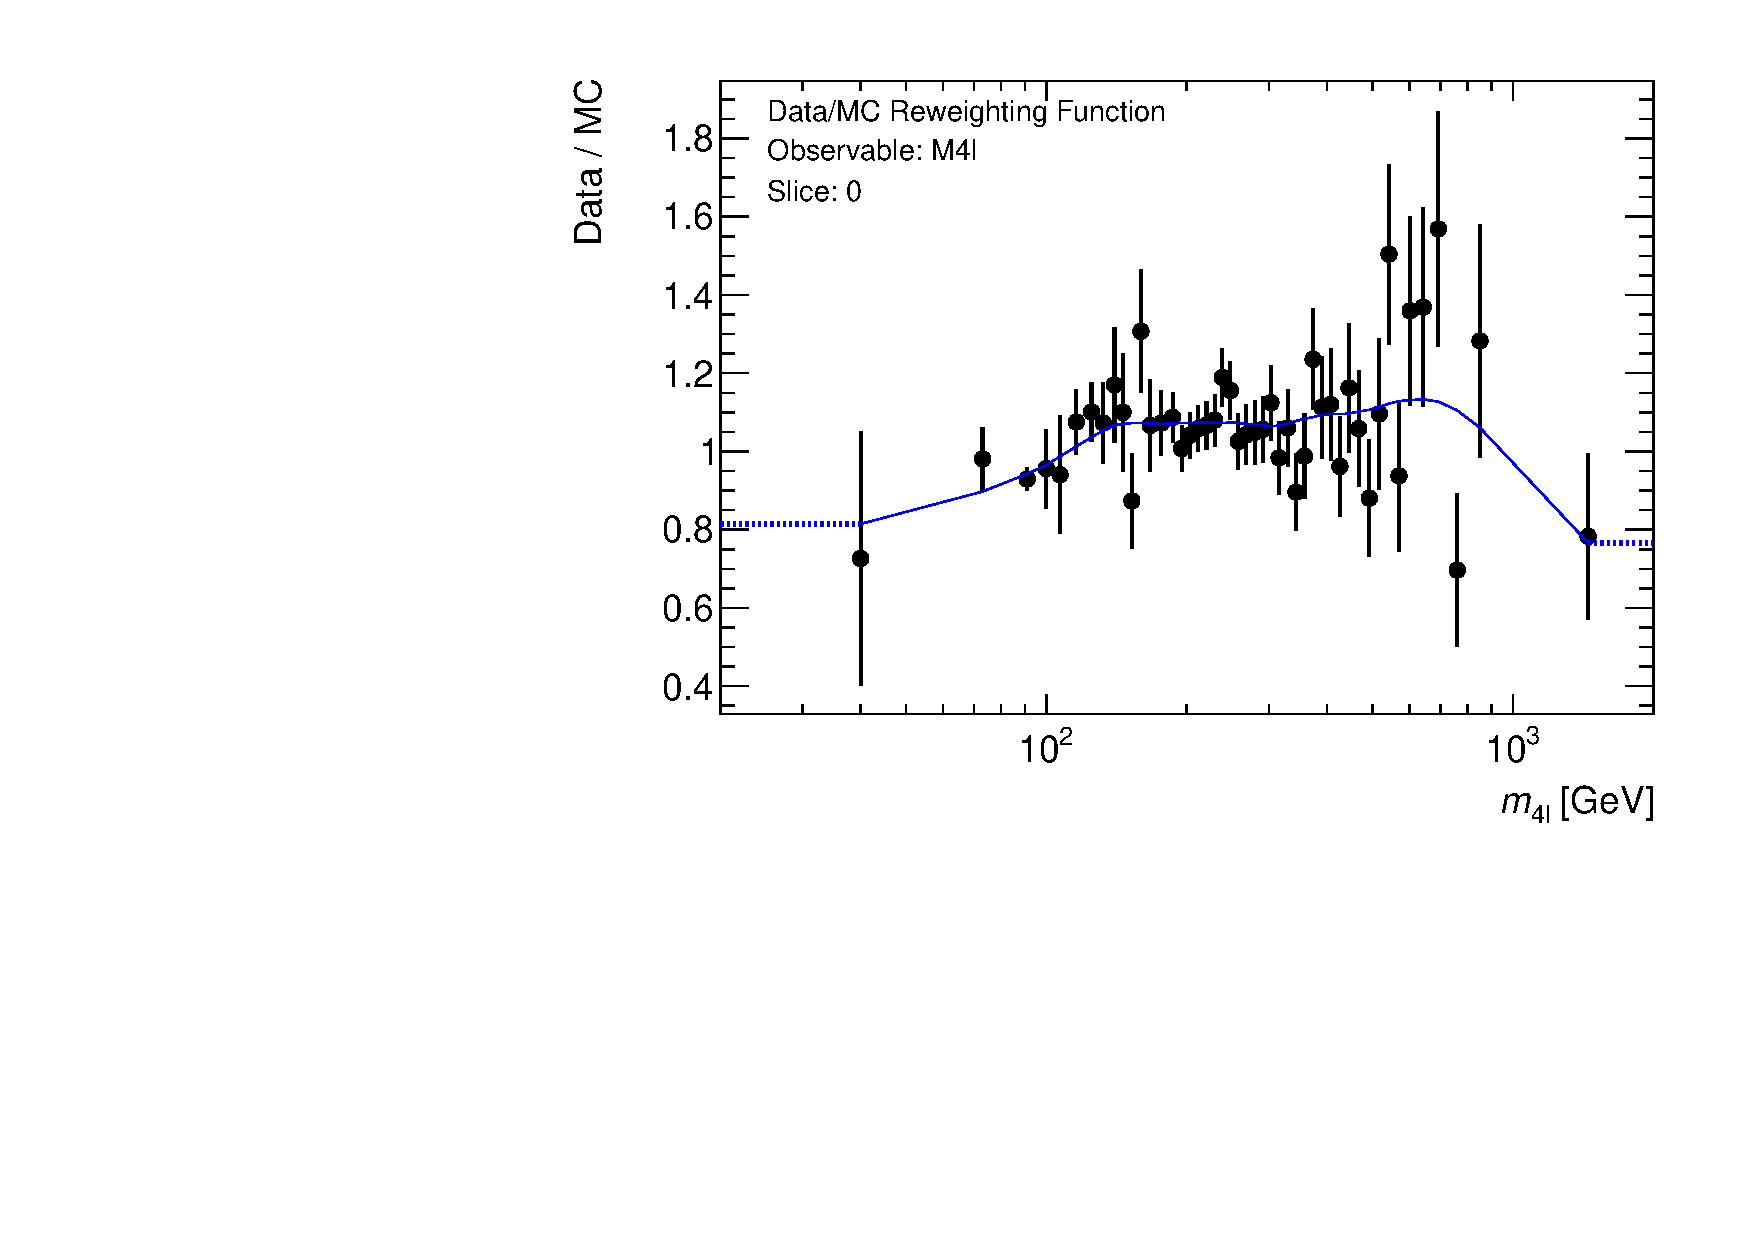
\includegraphics[width=.99\linewidth]{Figures/m4l/DataDriven/FitM4l-Slice0.pdf}\caption{}
    \end{subfigure}
    \begin{subfigure}{.49\textwidth}\centering
      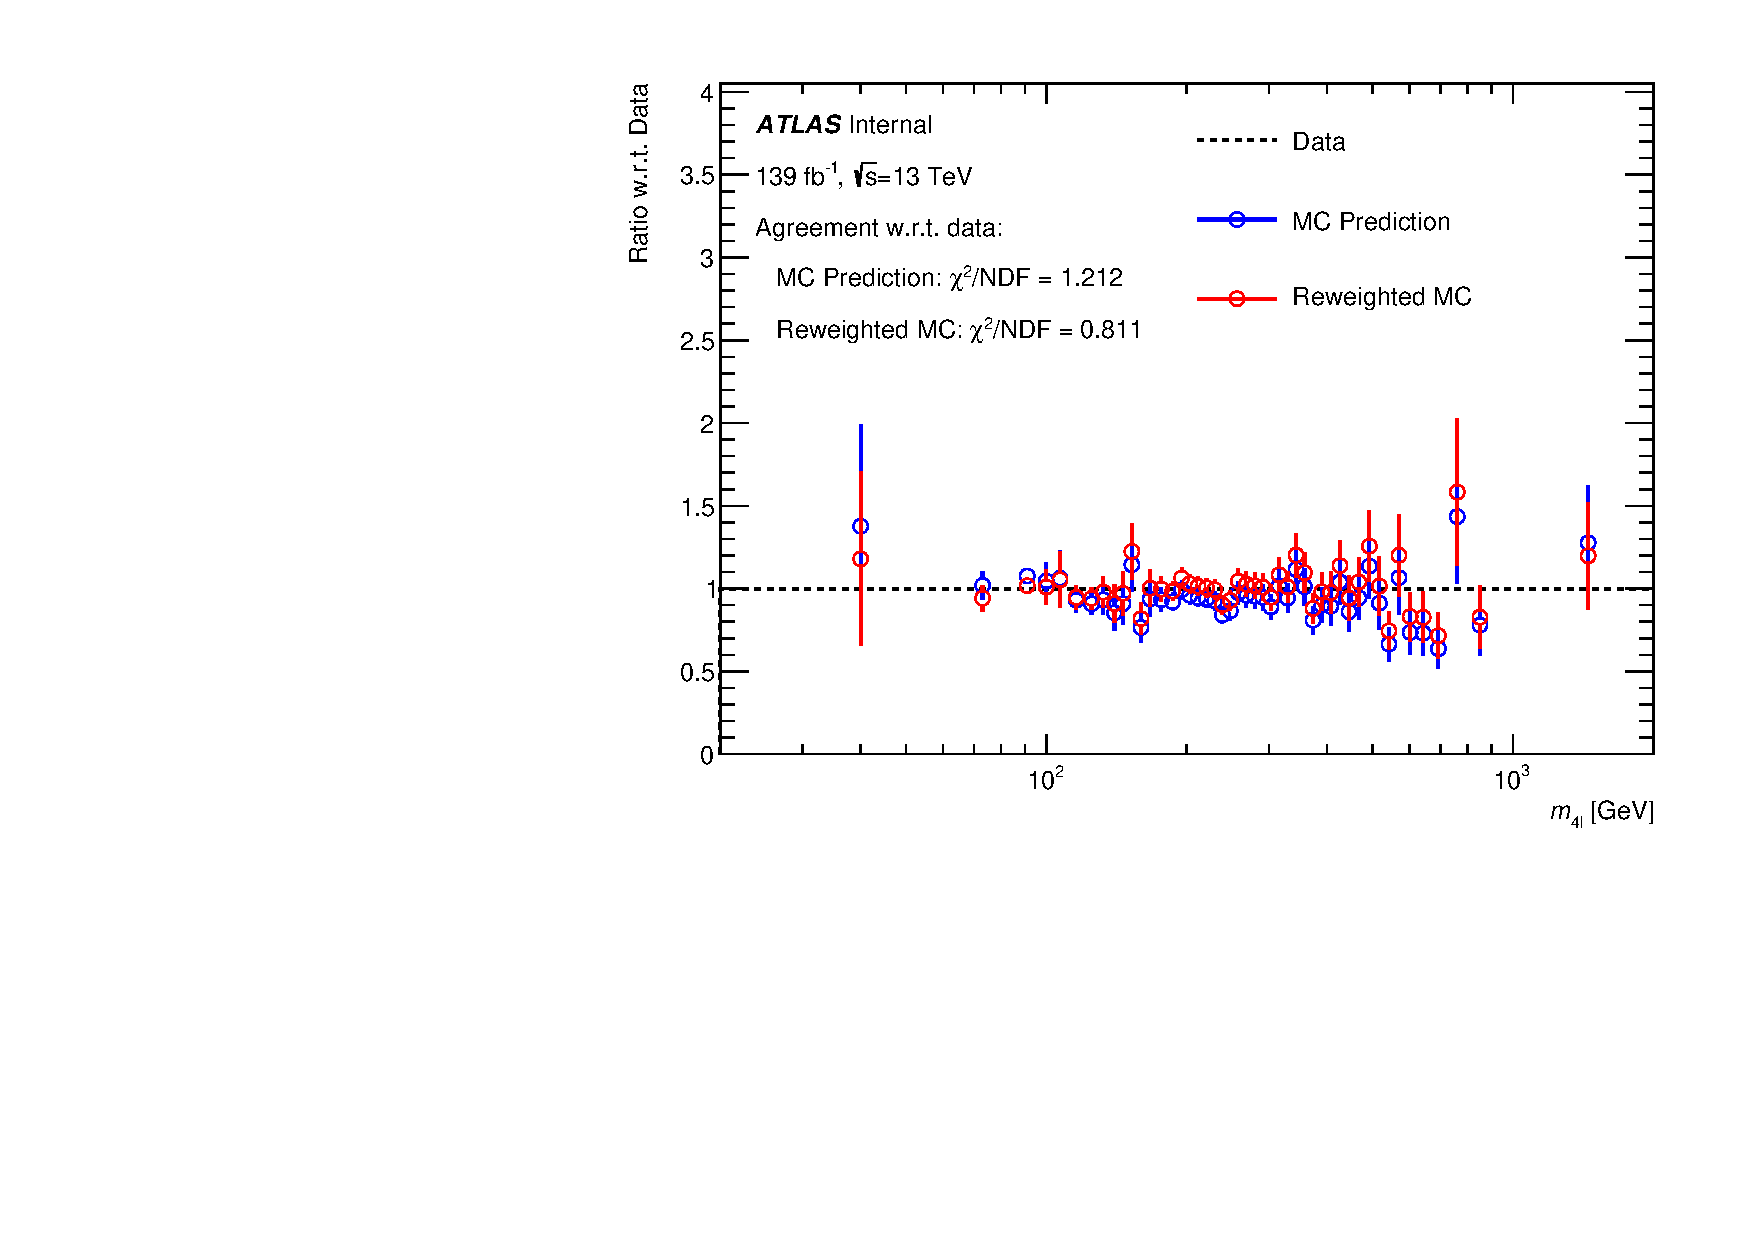
\includegraphics[width=.99\linewidth]{Figures/m4l/DataDriven/ReweightedM4l.pdf} \caption{}
    \end{subfigure}
    \begin{subfigure}{.49\textwidth}\centering
      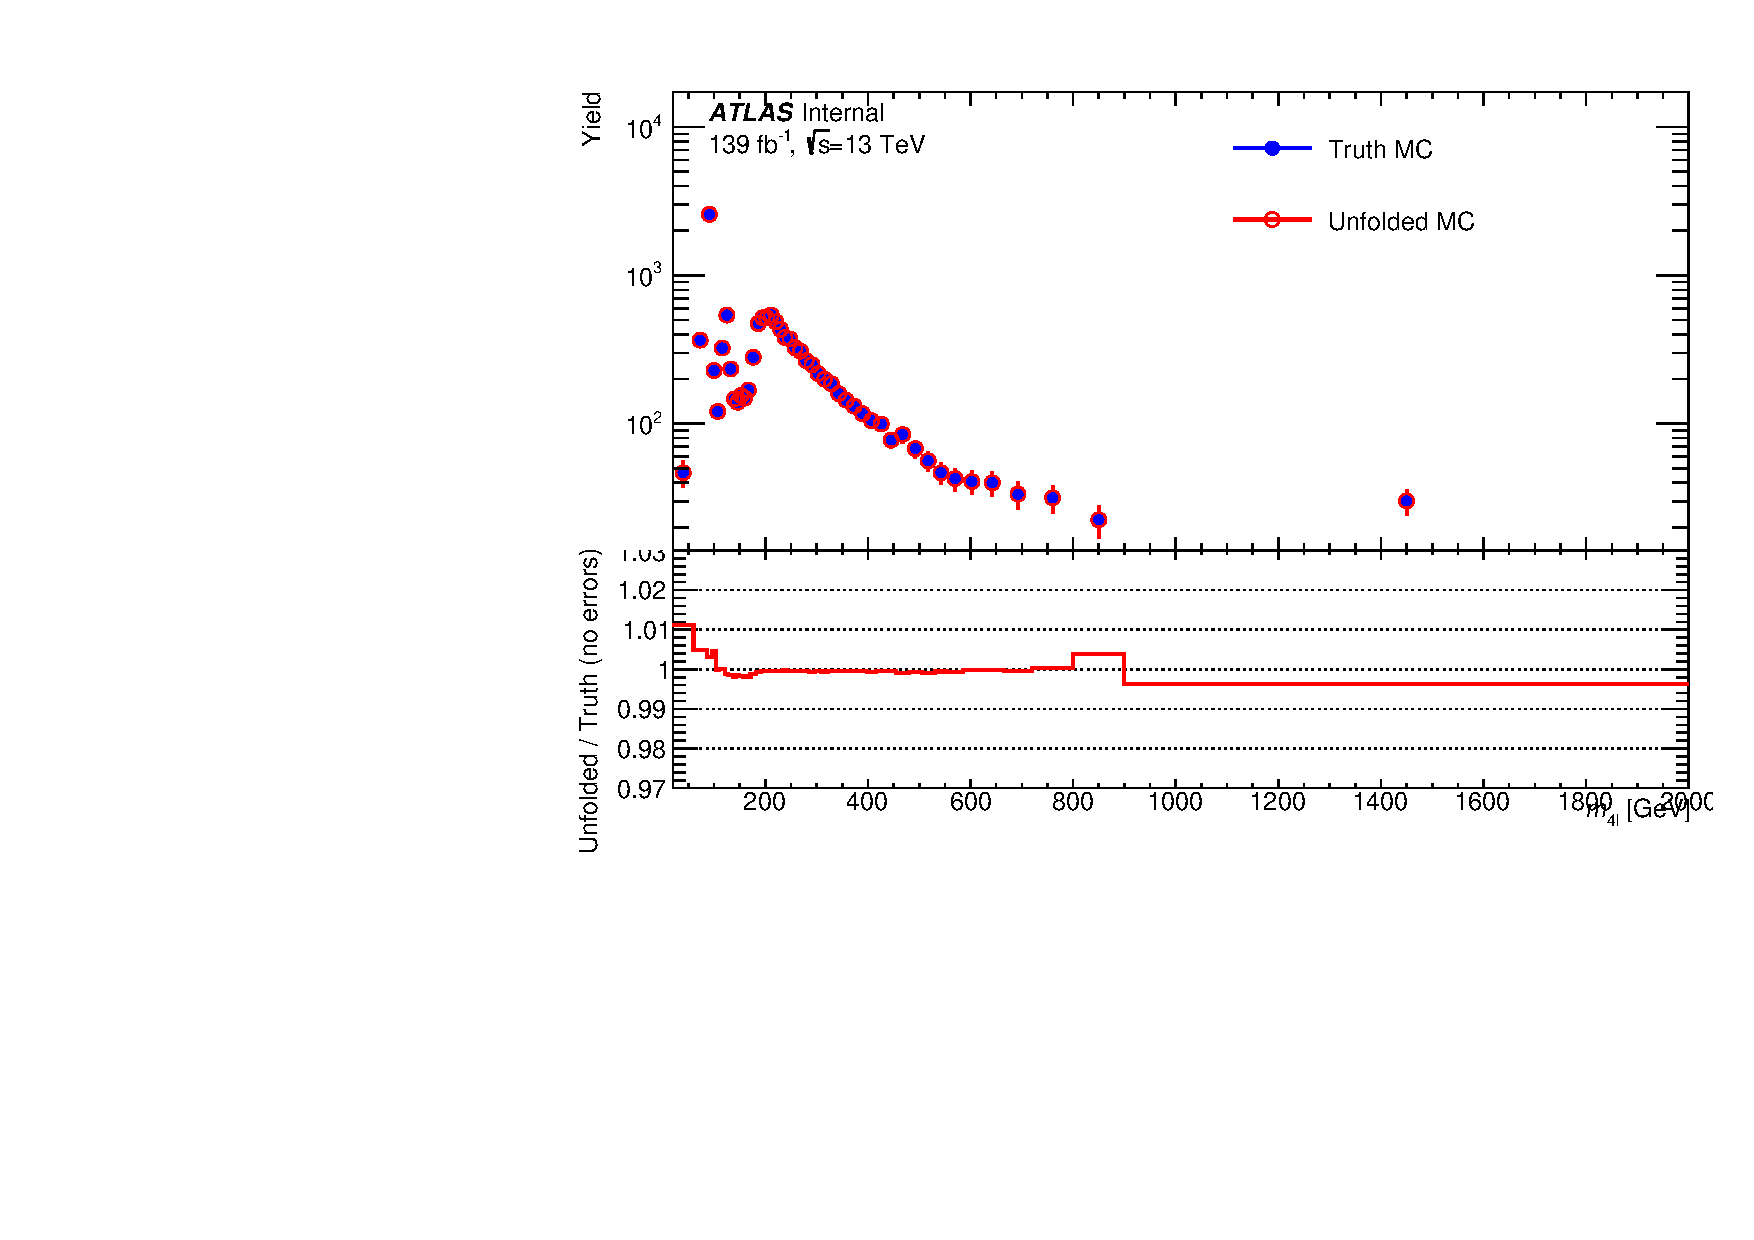
\includegraphics[width=.99\linewidth]{Figures/m4l/DataDriven/UnfoldedM4l.pdf}  \caption{}
    \end{subfigure}
    \caption{Step-by-step overview of the data-driven method for $\mFourL$. In (a), the observed data is compared to the nominal SM MC prediction at reconstruction-level. In (b), the reweighting function is obtained via smoothing of the data/MC ratio and is fixed to its last value in the final bins, as shown by the dashed lines. In (c), the truth-reweighted MC is compared to the nominal MC at reconstruction-level, showing, as expected, an improved agreement with the data. In (d), the difference in the ratio from unity is taken as the relative systematic uncertainty. \label{fig:m4ldatadriven}}
\end{figure}

\subsection{Injection studies}
\label{ssec:injectiontests}
Section \ref{ssec:closuretests} demonstrates that the unfolding procedure has closure when unfolding pseudo-data that agree with the Standard Model. Since the SM predictions themselves were used to derive the corrections and matrix used for unfolding, this is the expected case. The shape of real data is unknown, however, and may be different than the Standard Model prediction. Should the \mFourL spectrum be host to contributions that differ from the SM prediction, it is necessary to check that the unfolding procedure is nonetheless able to provide an accurate and unbiased particle-level result. In order to do this a number of injection tests were performed. The first step is to take the nominal SM prediction, and inject some amount of BSM signal into it. The reconstruction level yield of this modified sample is used as pseudo-data. It is run through the standard unfolding workflow in entirety, and compared to the particle level yield of the modified sample. Conceptually, this procedure is very similar to that of the Monte Carlo closure tests. 

A number of modifications were made to the nominal SM prediction, one set had the addition of a gluon-gluon fusion produced heavy Higgs boson with a mass of 300, 800, or \unit{1400}{\GeV} with either a narrow width or a width 15\% of its mass, and another set where the heavy Higgs was produced via vector-boson fusion. The \ggZZ process was also modified to have a larger event weight with respect to the SM prediction. These are described in full in Table \ref{tab:injectionsamples}. All of the models describe BSM scenarios with extremely large enhancements or resonances. 
\begin{table}[tbp]
    \begin{tabular}{lll}
                            & Injection samples & \\
        \midrule \\
                            &               & 300 GeV \\
         Gluon-gluon fusion &  Narrow width & 800 GeV\\
                            &               & 1400 GeV \\
                            &               & 300 GeV \\
                            & 15\% width    & 800 GeV \\
                            &               & 1400 GeV \\
         \midrule \\
                                & & 300 GeV \\
         Vector-boson fusion    & & 800 GeV \\
                                & & 1400 GeV \\
         \midrule \\
         \ggZZ Enhancement & \\
    \end{tabular}
  \caption{Modifications made to the nominal SM prediction for injection studies.}
  \label{tab:injectionsamples}
\end{table}

For each of the variations listed in Table \ref{tab:injectionsamples}, a range of cross-sections were injected and then unfolded with and without application of the pre-unfolding weights. In order to carve a more realistic scenario, one of the injected cross-sections for the heavy Higgs samples was set to be just within the two-sigma band of the data uncertainty. This was done by increasing the injected cross-section and calculating the $p$-value between the BSM prediction and the data until a $p$-value smaller than or equal to 0.05 is reached. This is the $p$-value corresponding to a two-sigma significance. The results from the injection tests corresponding to a two-sigma injected amount for all the gluon-gluon fusion BSM samples are shown in Figure~\ref{fig:m4l:injection}. The nominal SM prediction and the modified BSM + SM prediction at particle level are shown (SM truth and BSM truth respectively), along with two unfolded BSM distributions, one with pre-unfolding (pre-UF) weights applied and one without. The lower panel is the ratio of the unfolded BSM distribution to the true BSM distribution and is interpreted as the bias. 

Figure~\ref{fig:injection_6dot175fb_300w15} is also published in Reference~\cite{m4l2021_paper}. It shows the result of the injection test using a BSM model with a resonance mass of $m_{\mathrm{res}}=300~\GeV{}$ and width 15\% of the mass, with a cross-section of \unit{6.18}{\invfb}. Looking at the ratio panel, the bias goes up to 2.2\% without the application of the pre-unfolding weights (in green). With the weights applied, the bias is smaller and remains within a $\pm0.8\%$ range (in black). The same trend holds true for the rest of the 15\% width samples, see Figures~\ref{fig:injection_0dot862fb_800w15}-\ref{injection_0dot4032fb_1400w15}. Application of the pre-unfolding weights tend to result in a smaller bias, especially for 300~\GeV and 800~\GeV resonances. For the highest resonance mass at 1400~\GeV, the pre-unfolding has a notable effect only in the last \mFourL mass bin, where it reduces the bias from 10\% to 4\%.

The gluon-gluon fusion narrow-width heavy Higgs models' injection test results are presented in Figures~\ref{fig:injection_1dot24fb_300NW}-\ref{fig:injection_0dot19fb_1400NW}. The unfolding method is much more sensitive to, and therefore less robust to, the presence of narrow resonances. Here, the pre-unfolding is not as effective in mitigating the effects of the BSM signal. The differences between the unfolded BSM and the truth BSM, however, is still within 6\% bias for the 300~\GeV and 1400~\GeV resonance mass models. For the 800~\GeV model this goes up to 16\%. In all cases, the bias is well within the total uncertainty in the corresponding \mFourL mass bin. 

\begin{figure}[htb]
    \begin{subfigure}{.49\textwidth}\centering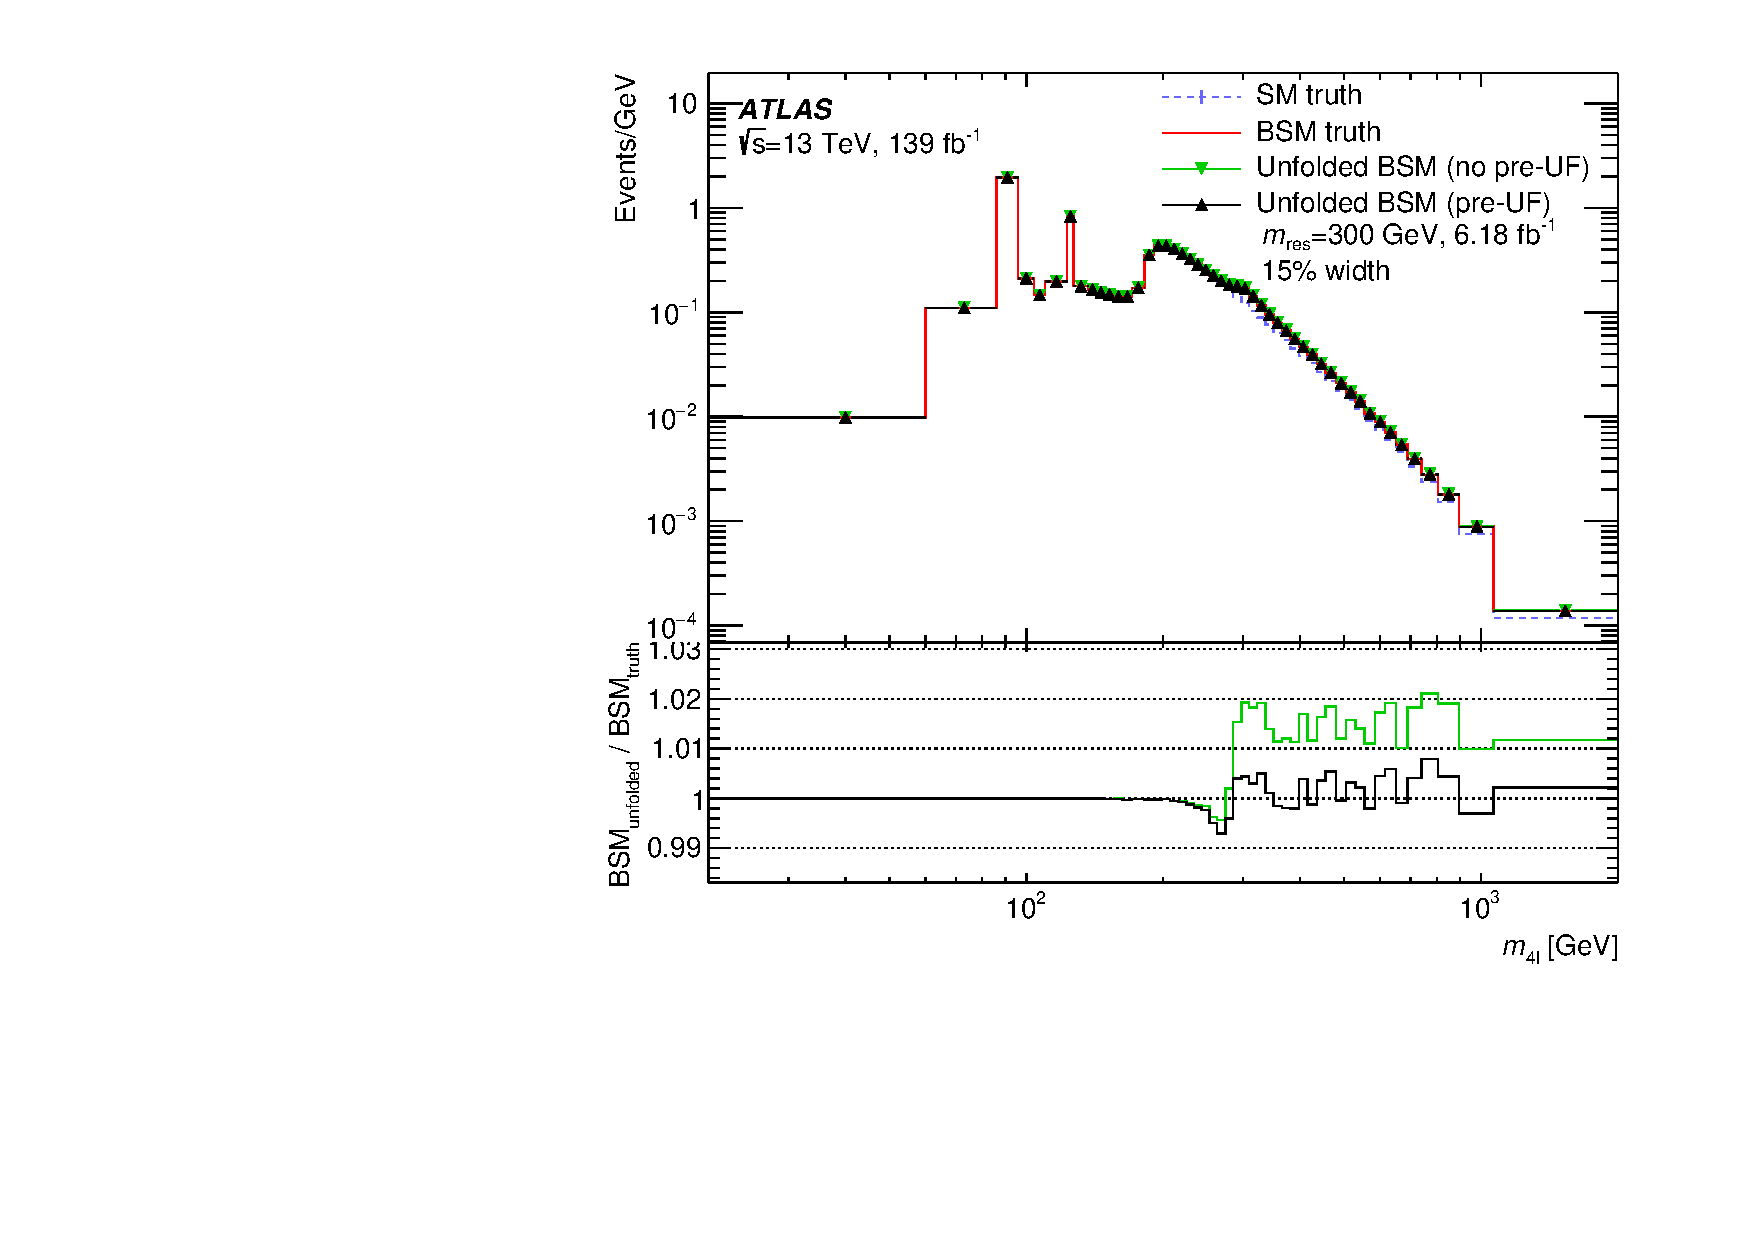
\includegraphics[width = 0.95\textwidth]{Figures/m4l/InjectionTests/6dot175fb_300w15_injection.pdf}\caption{}\label{fig:injection_6dot175fb_300w15}\end{subfigure}
    \begin{subfigure}{.49\textwidth}\centering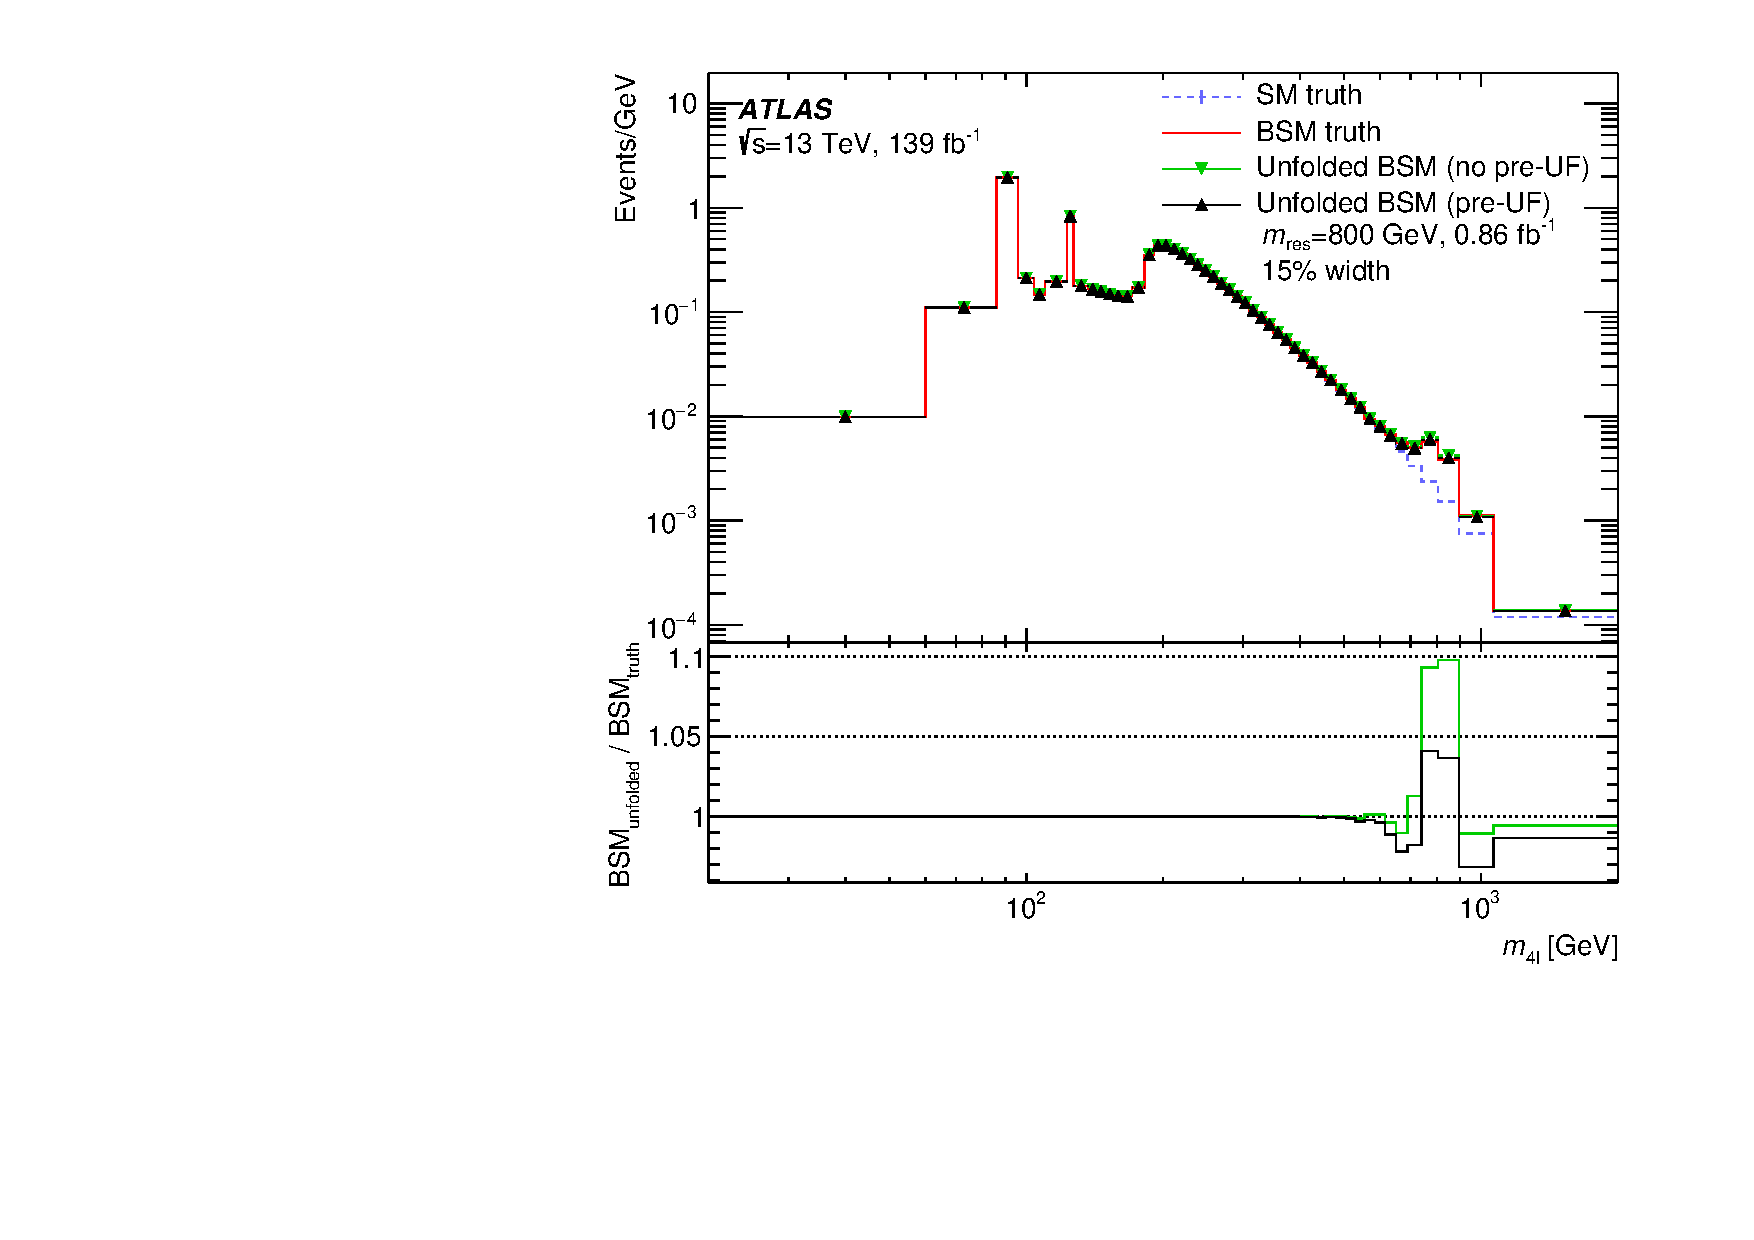
\includegraphics[width = 0.95\textwidth]{Figures/m4l/InjectionTests/0dot862fb_800w15_injection.pdf}\caption{}\label{fig:injection_0dot862fb_800w15}\end{subfigure}
    \begin{subfigure}{.49\textwidth}\centering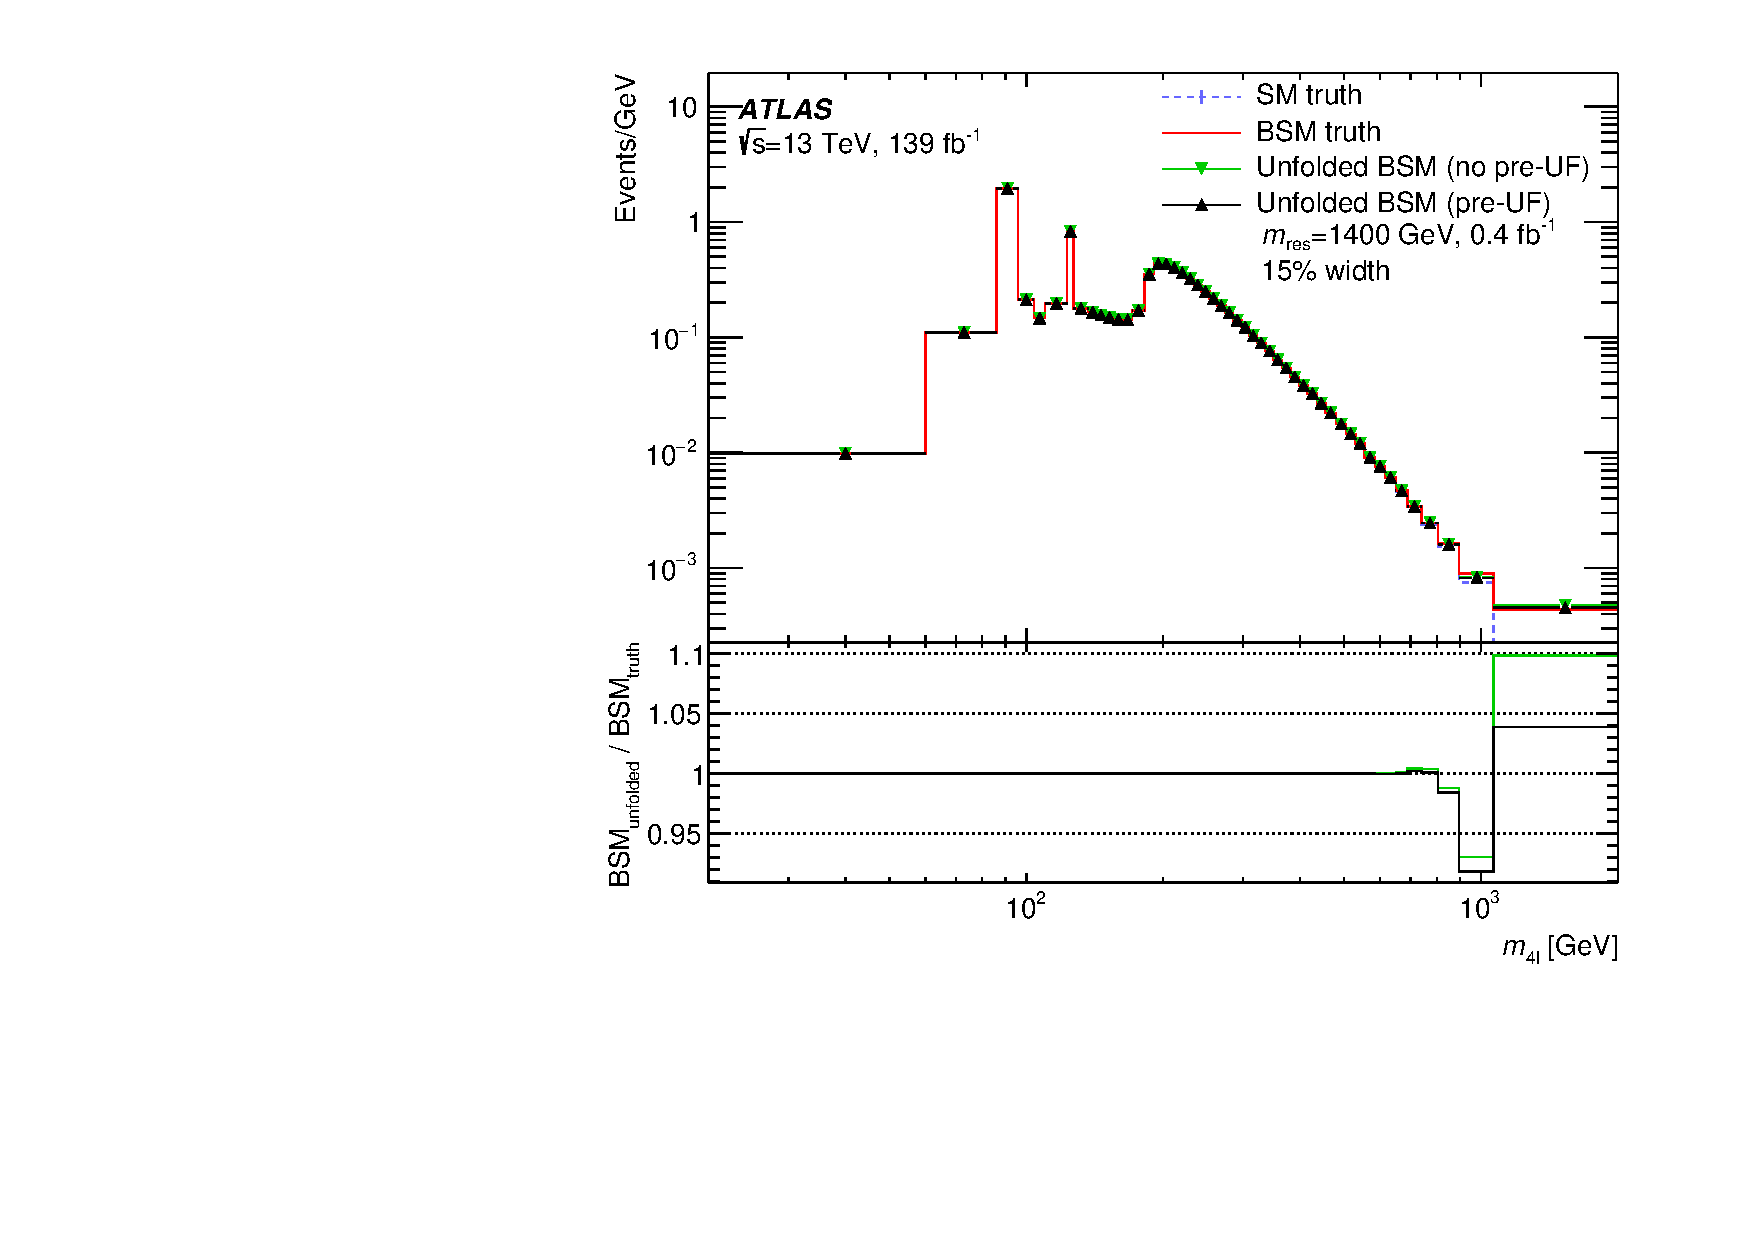
\includegraphics[width = 0.95\textwidth]{Figures/m4l/InjectionTests/0dot4032fb_1400w15_injection.pdf}\caption{}\label{fig:injection_0dot4032fb_1400w15}\end{subfigure}
    \begin{subfigure}{.49\textwidth}\centering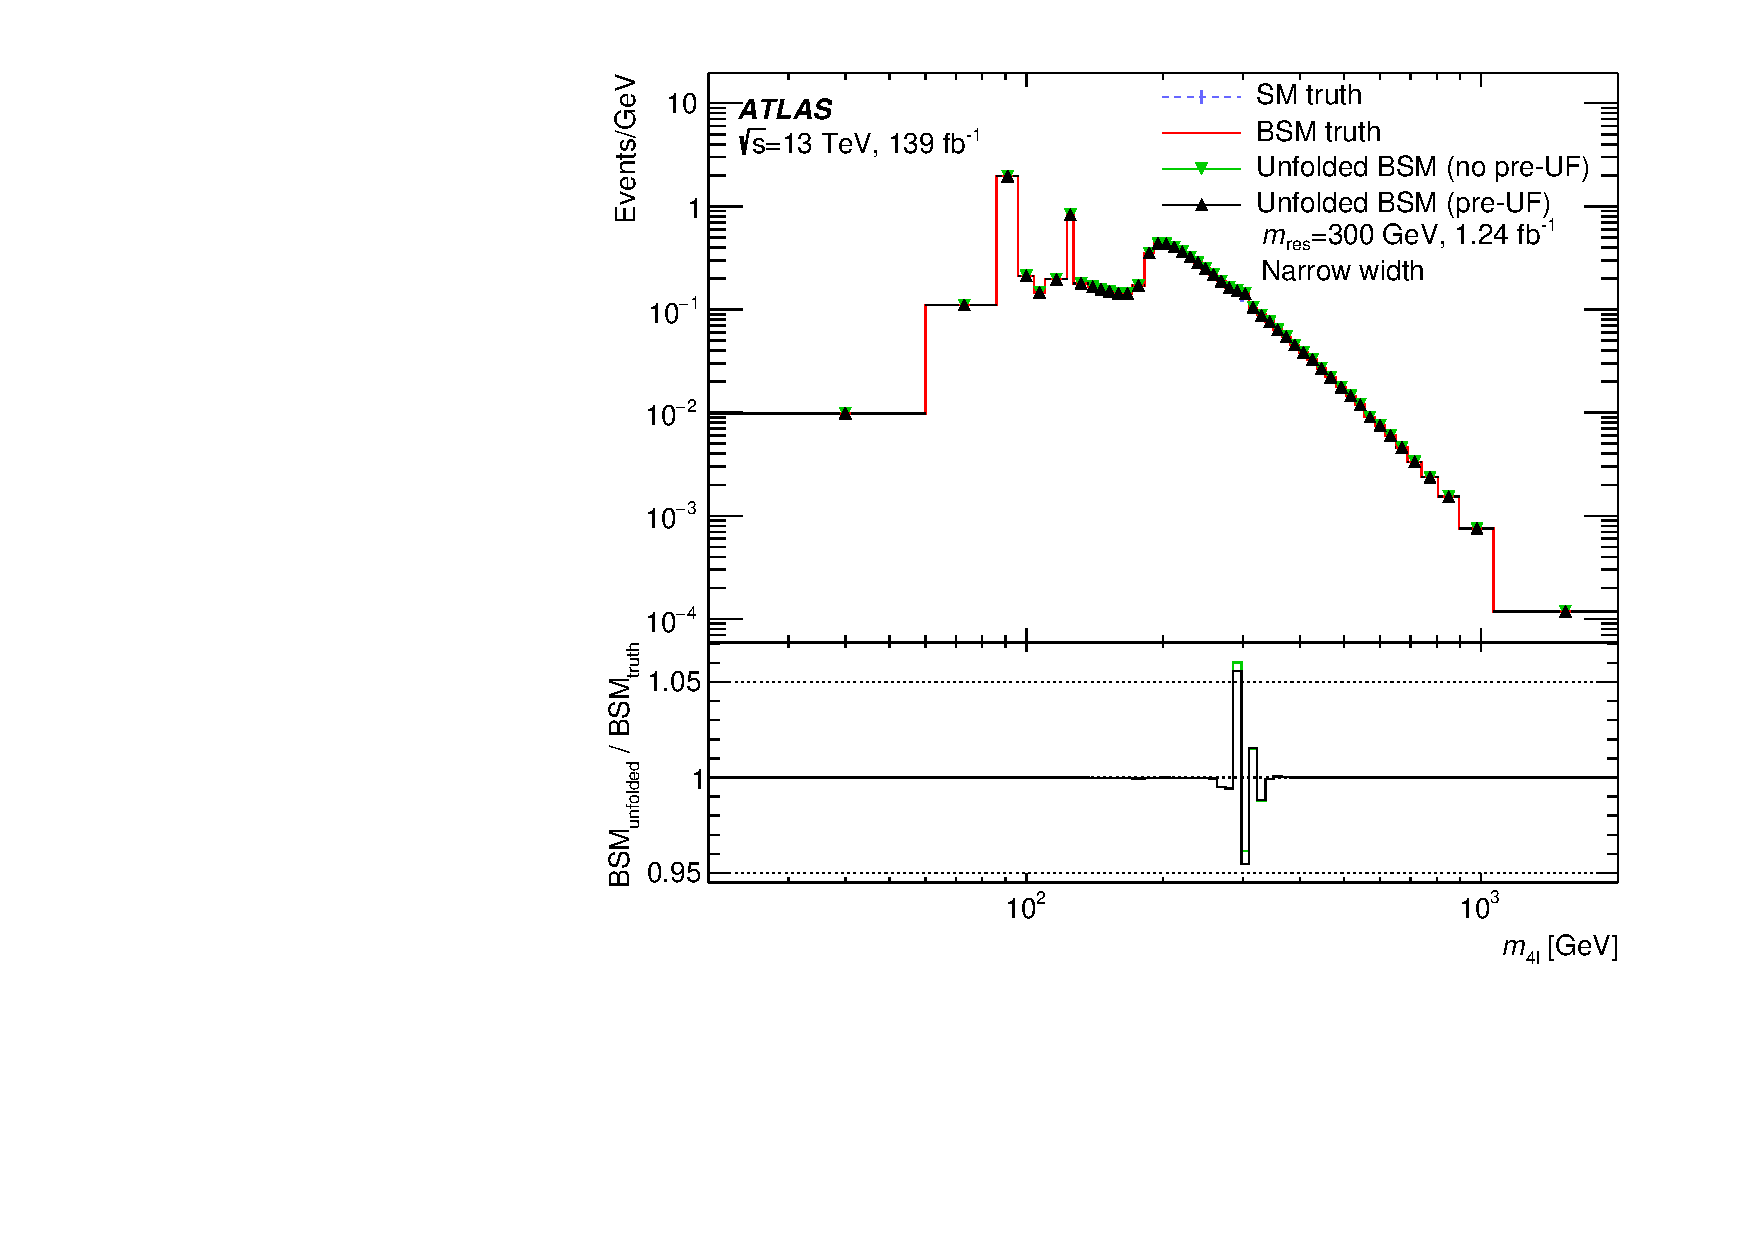
\includegraphics[width = 0.95\textwidth]{Figures/m4l/InjectionTests/1dot24fb_300NW_injection.pdf}\caption{}l\label{fig:injection_1dot24fb_300NW}\end{subfigure}
    \begin{subfigure}{.49\textwidth}\centering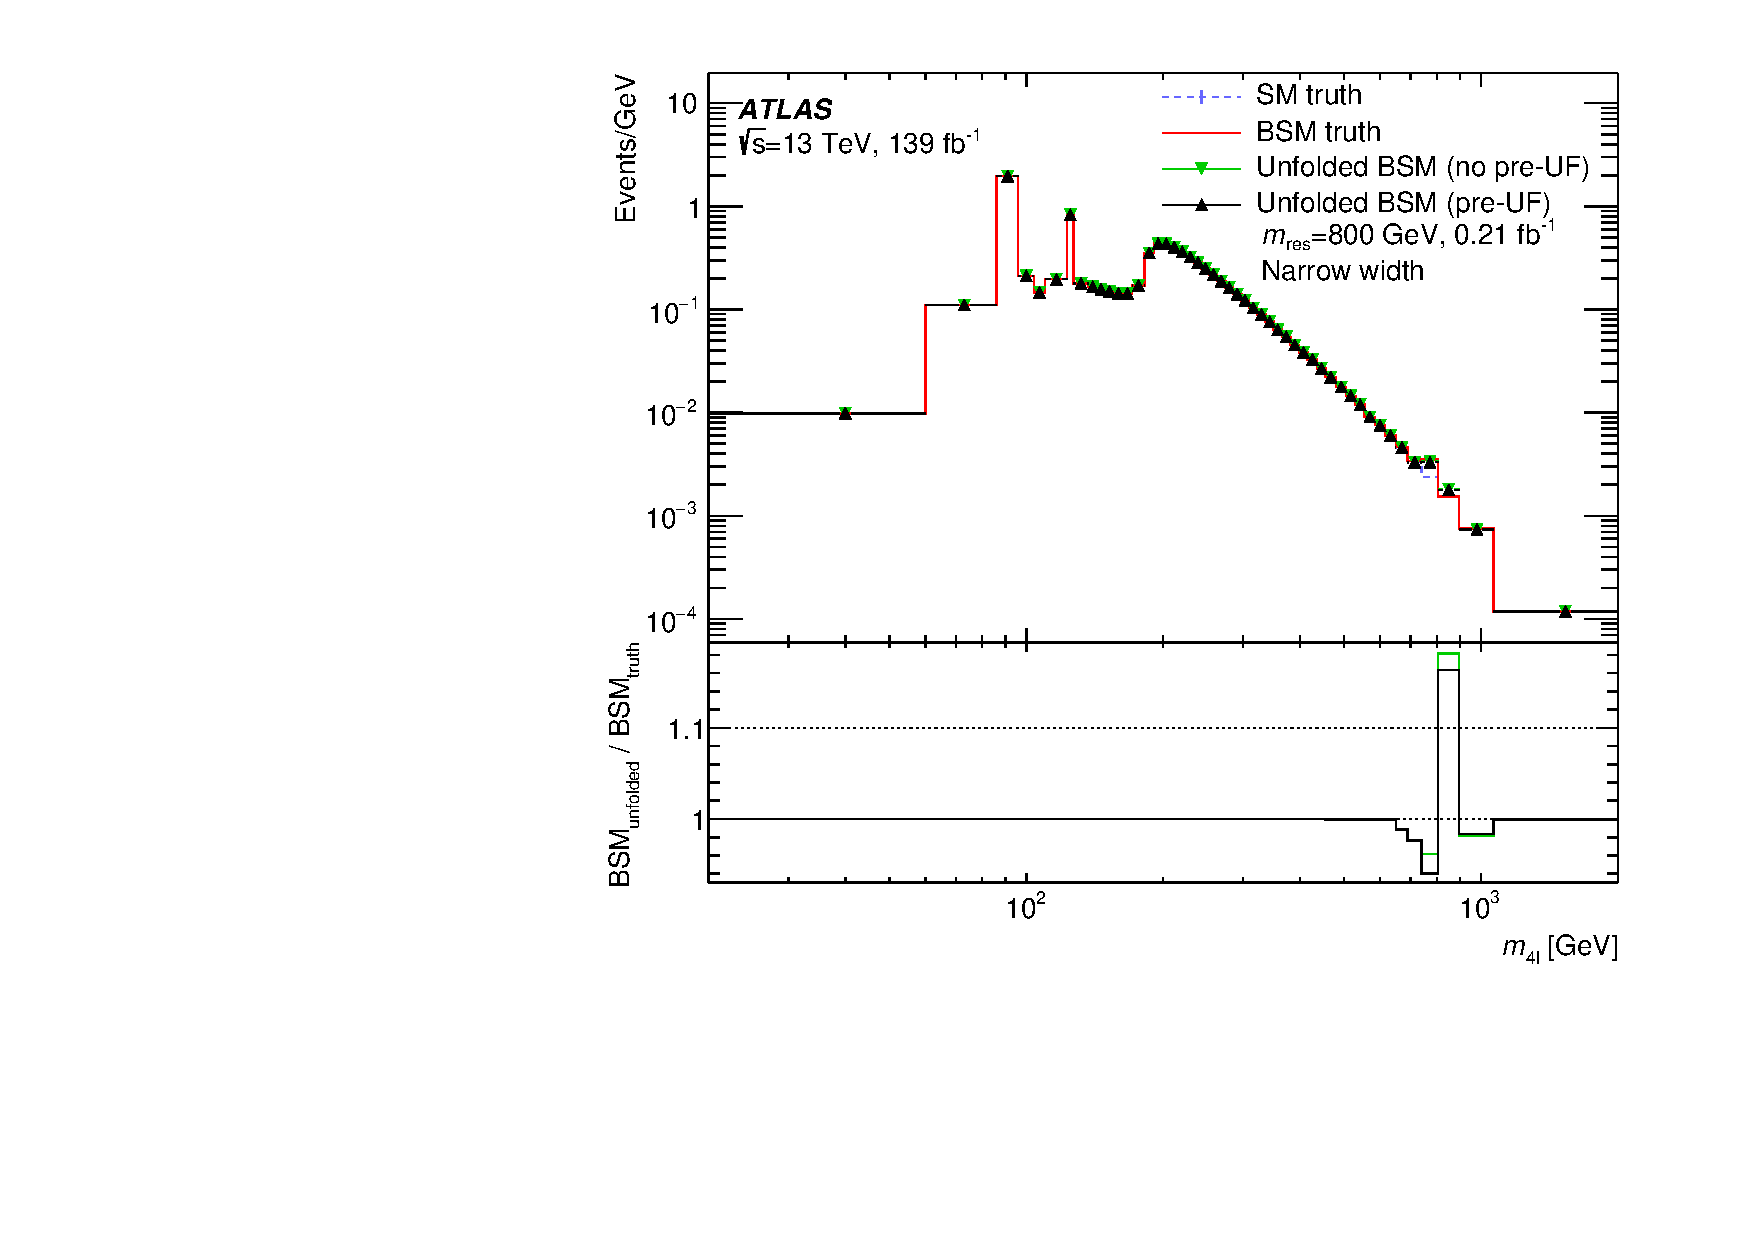
\includegraphics[width = 0.95\textwidth]{Figures/m4l/InjectionTests/0dot212fb_800NW_injection.pdf}\caption{}\end{subfigure}
    \begin{subfigure}{.49\textwidth}\centering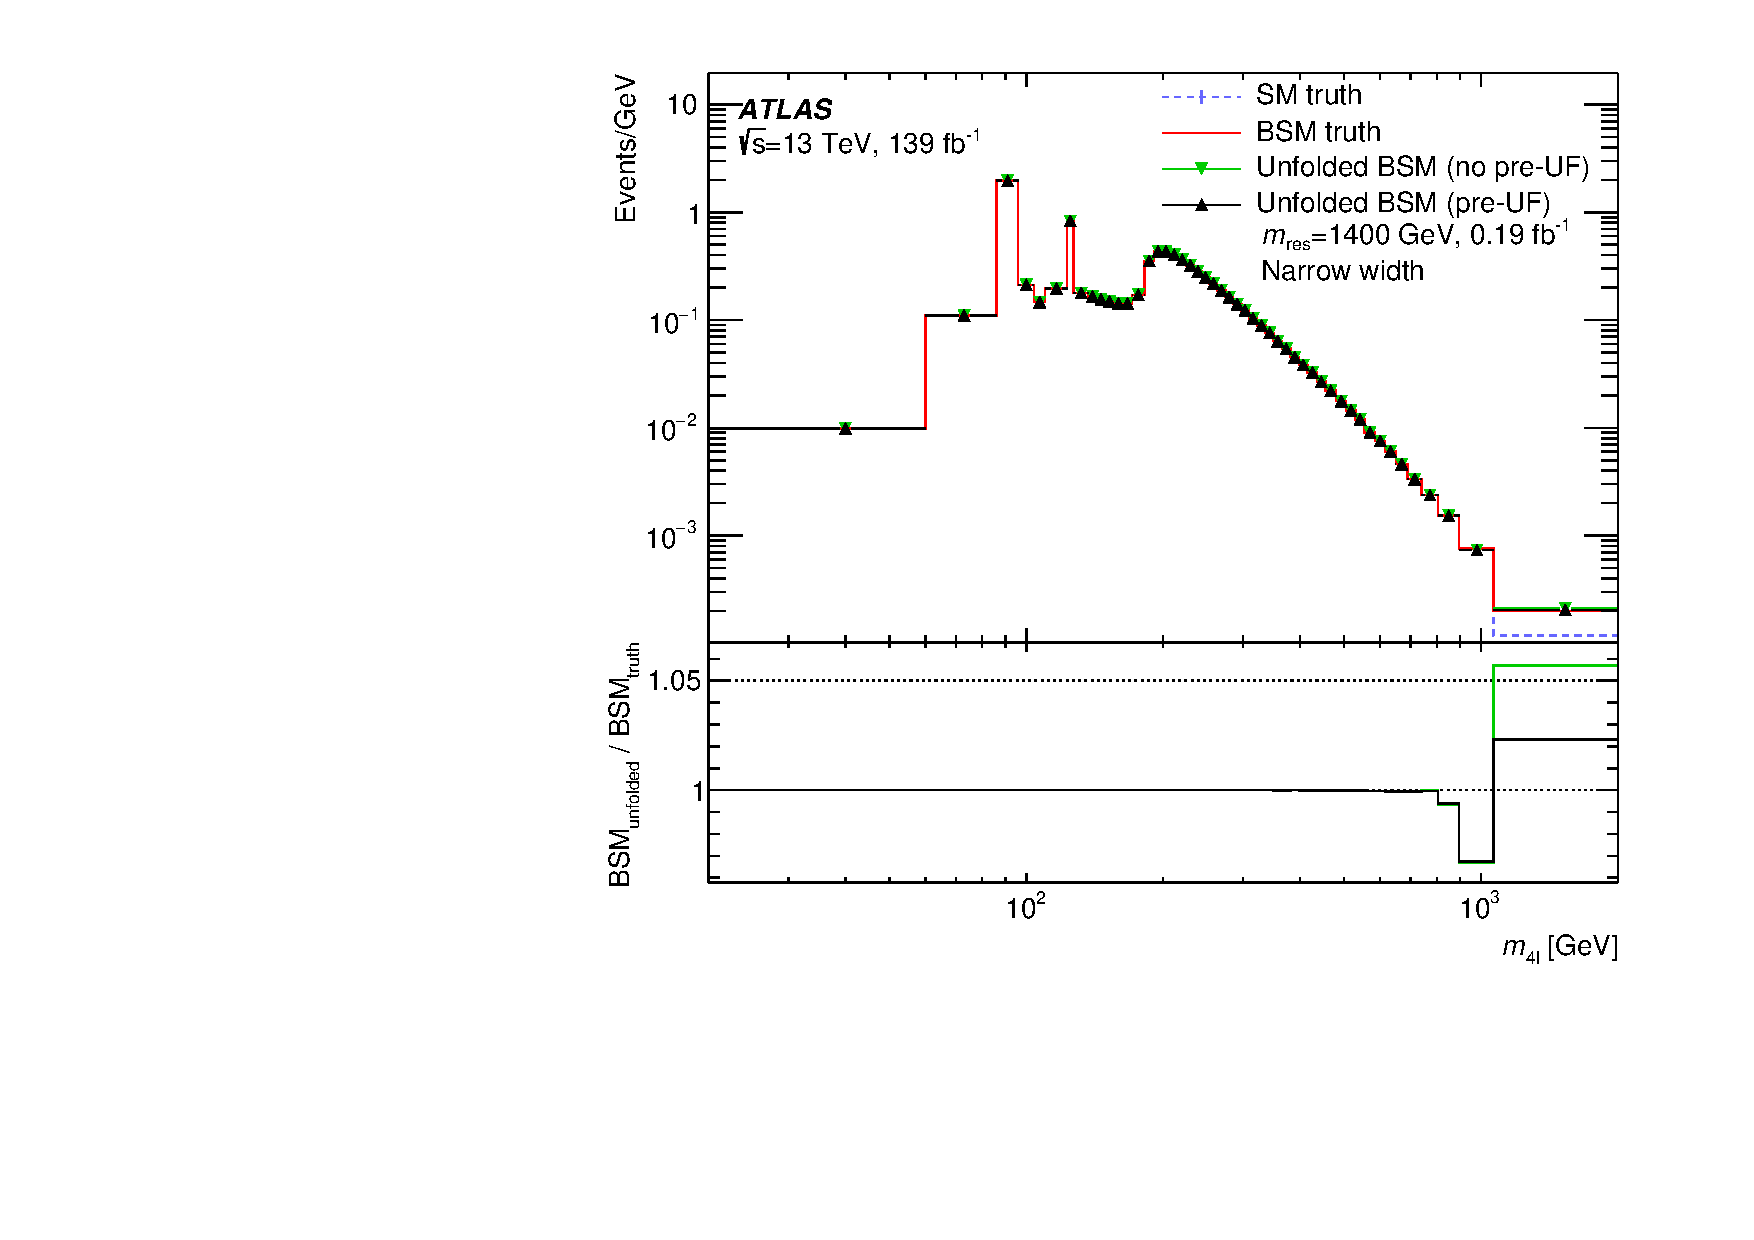
\includegraphics[width = 0.95\textwidth]{Figures/m4l/InjectionTests/0dot19fb_1400NW_injection.pdf}\caption{}\label{fig:injection_0dot19fb_1400NW}\end{subfigure}
    \caption{This figure shows the results of the BSM signal injection studies performed on the \mFourL distribution. Six BSM models are considered, with resonance masses at 300~\GeV, 800~\GeV, and 1400~\GeV, and with narrow widths or a width 15\% of the resonance mass. The cross-sections correspond to a $2\sigma$ signal significant with respect to the data uncertainty. Two unfolded distributions are shown with and without pre-unfolding (pre-UF) weights applied. The bottom panel shows the size of the bias.}
    \label{fig:m4l:injection}
\end{figure}
  \section{Measurement uncertainties}
\label{sec:uncertainties}
An important aspect of an experimental measurement is characterizing its uncertainty. Broadly speaking, uncertainties can be divided into two types. The first is the statistical uncertainty, which is caused by inherently unpredictable fluctuations and can be reliably estimated by making repeated measurements~\cite{Kar:ab1be6}. The second is the category of systematic uncertainties, which arise in the estimation of systematic effects such as background, selection bias, scanning efficiency, energy resolution, angle resolution, variation of counter efficiency with beam position and energy, dead time, etc\cite{orear}. Systematic uncertainties are generally more difficult to determine, and cannot be calculated simply from sampling fluctuations \cite{reygers}. The total uncertainty of the measurement is the sum in quadrature of each individual component.

The breakdown and contribution of the uncertainty sources is shown in Figure \ref{fig:m4lsystematics} for the inclusive \mFourL{} spectrum. The dominant is the statistical uncertainty in all but the third mass bin with resonant single $Z$ production, where the lepton efficiencies' uncertainty prevails. Table \ref{tab:SysTablePerSlice} shows the breakdown of the uncertainties on the total fiducial unfolded cross-section, as well as the fiducial cross-section in the four \mFourL{} regions. The data statistical uncertainty plays a dominant role, followed by the uncertainty from the choice of generator. The rest of this section will discuss the different sources of uncertainty and how they are propagated.

\begin{figure}
    \centering
    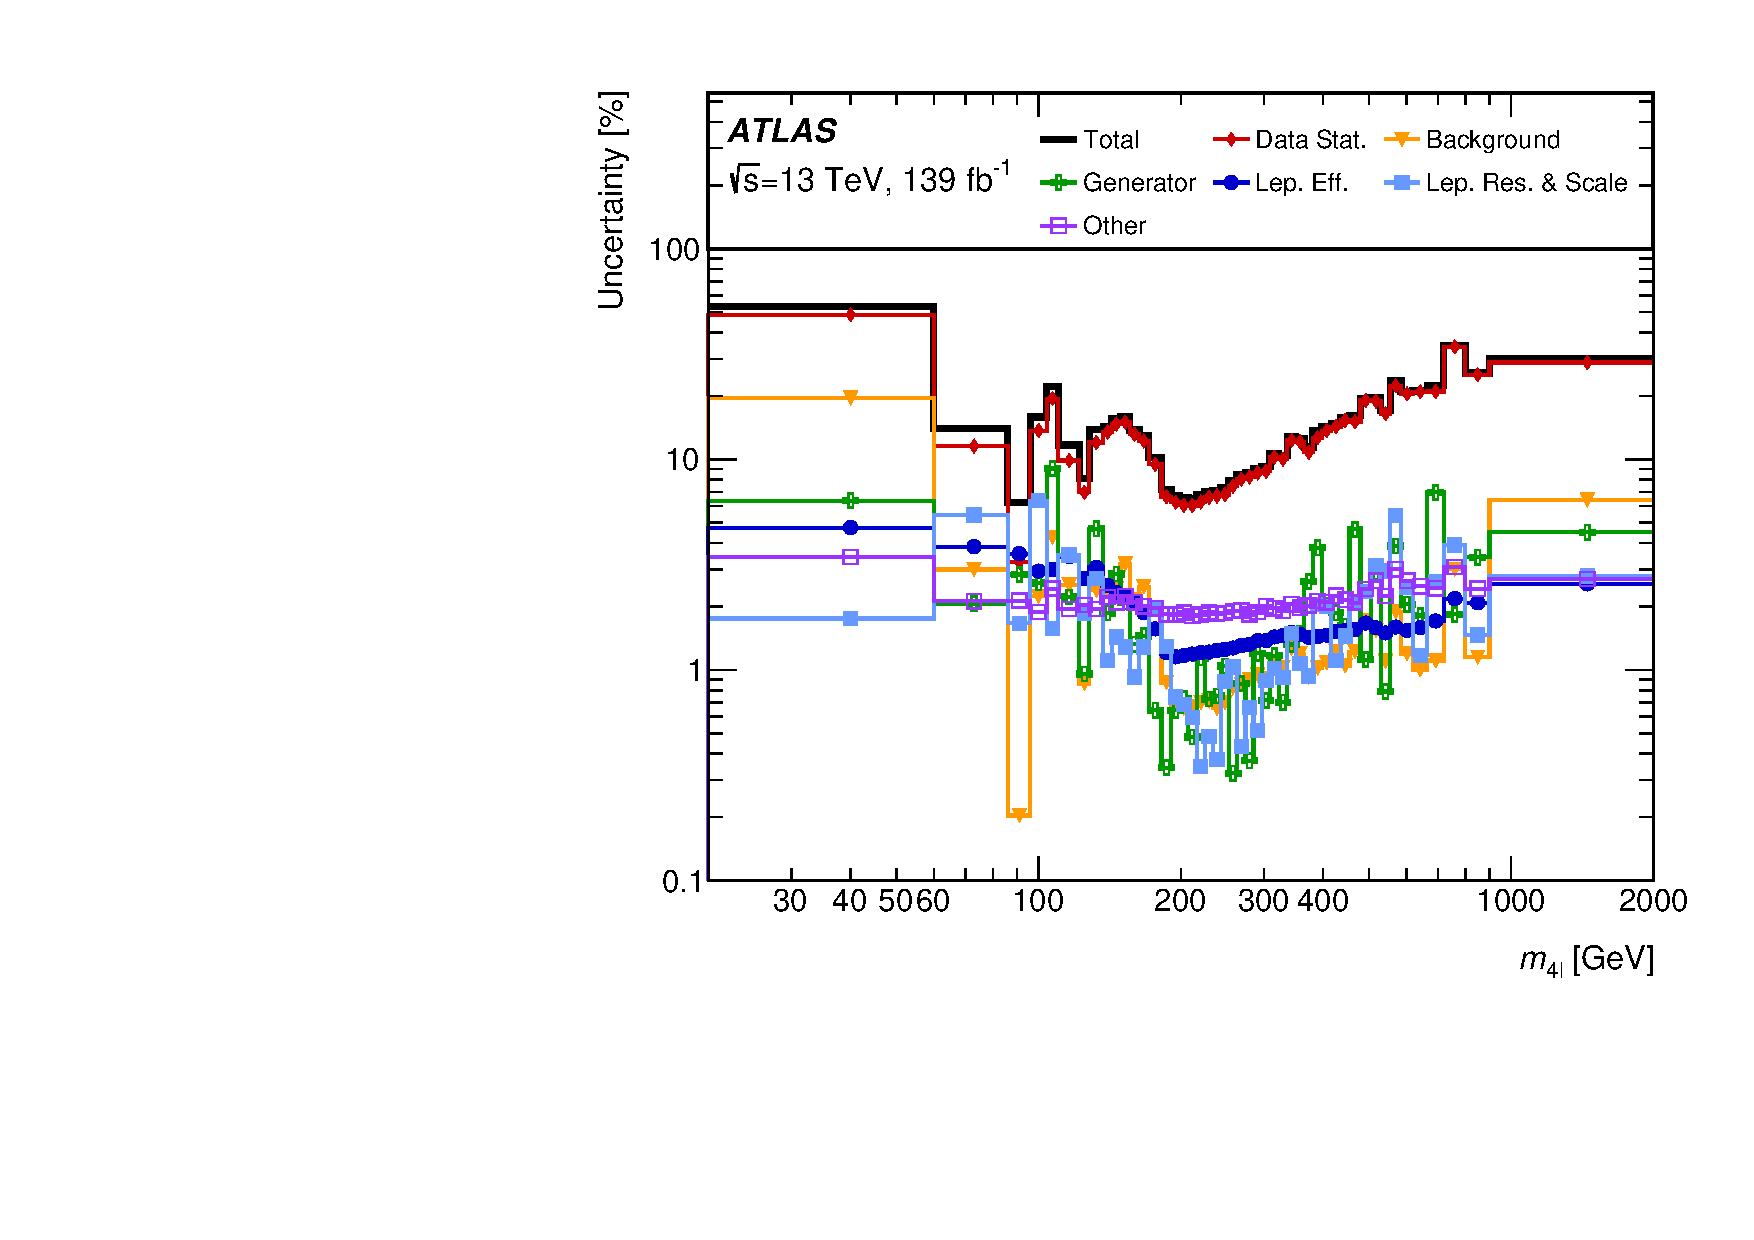
\includegraphics[width=0.85\textwidth]{Figures/m4l/Systematics/UnfoldedSys_M4l_Stack_Paper.pdf}
    \caption{Unfolded systematics for the inclusive \mFourL{} spectrum. The data statistical uncertainty is the dominant source in all but the third bin. This figure is from Ref.~\cite{m4l2021_paper}}
    \label{fig:m4lsystematics}
\end{figure}
\begin{table}
    \centering 
     \begin{tabular} {c  c  c  c  c  c }
         \hline 
         Region  & Inclusive   & $Z\rightarrow 4\ell$   & on-shell $H$   & off-shell $ZZ$   & on-shell $ZZ$   \\
         $m_{4\ell}$ [GeV]  & any   & 60-100   & 120-130   & 20-60/100-120   & 180-2000   \\
            &       &       &       & /130-180 & \\
         \hline 
        DD Closure &  $ 0.088\% $  &  $ 0.35\% $  &  $ 0.13\% $  &  $ 0.45\% $  &  $ 0.035\% $ \\
        Electron ID &  $ 0.94\% $  &  $ \mathbf{1.9}\% $  &  $ \mathbf{1.5}\% $  &  $ \mathbf{1.3}\% $  &  $ 0.49\% $ \\
        Electron Isolation &  $ 0.52\% $  &  $ \mathbf{1.1}\% $  &  $ 0.79\% $  &  $ 0.73\% $  &  $ 0.18\% $ \\
        Electron Reco &  $ 0.84\% $  &  $ \mathbf{1.7}\% $  &  $ \mathbf{1.3}\% $  &  $ \mathbf{1.2}\% $  &  $ 0.31\% $ \\
        Electron Res. \& Scale &  $ 0.46\% $  &  $ \mathbf{1.1}\% $  &  $ 0.83\% $  &  $ 0.54\% $  &  $ 0.12\% $ \\
        Generator &  $ \mathbf{1.3}\% $  &  $ \mathbf{2.6}\% $  &  $ \mathbf{1.3}\% $  &  $ \mathbf{2.7}\% $  &  $ 0.13\% $ \\
        MC Stat. &  $ 0.087\% $  &  $ 0.22\% $  &  $ 0.38\% $  &  $ 0.26\% $  &  $ 0.088\% $ \\
        Muon Isolation &  $ 0.96\% $  &  $ \mathbf{1.6}\% $  &  $ \mathbf{1.2}\% $  &  $ \mathbf{1.2}\% $  &  $ 0.58\% $ \\
        Muon Reco \& ID &  $ 0.83\% $  &  $ \mathbf{1.1}\% $  &  $ 0.91\% $  &  $ 0.89\% $  &  $ 0.82\% $ \\
        Muon Res. \& Scale &  $ 0.3\% $  &  $ 0.65\% $  &  $ 0.55\% $  &  $ 0.53\% $  &  $ 0.13\% $ \\
        Muon TTVA &  $ 0.21\% $  &  $ 0.46\% $  &  $ 0.28\% $  &  $ 0.31\% $  &  $ 0.071\% $ \\
        Non-Generator Theory &  $ 0.27\% $  &  $ 0.31\% $  &  $ 0.23\% $  &  $ 0.45\% $  &  $ 0.27\% $ \\
        Pile-up &  $ 0.73\% $  &  $ \mathbf{1.2}\% $  &  $ \mathbf{1}\% $  &  $ 0.81\% $  &  $ 0.47\% $ \\
        Reducible &  $ 0.8\% $  &  $ 0.55\% $  &  $ \mathbf{1.7}\% $  &  $ \mathbf{2.5}\% $  &  $ 0.74\% $ \\
        Trigger &  $ 0.33\% $  &  $ 0.8\% $  &  $ 0.44\% $  &  $ 0.44\% $  &  $ 0.084\% $ \\
        \hline 
        Total Systematic &  $ 2.6\% $  &  $ 4.8\% $  &  $ 3.7\% $  &  $ 4.6\% $  &  $ 1.5\% $ \\
        Luminosity &  $ \mathbf{1.7}\% $  &  $ \mathbf{1.6}\% $  &  $ \mathbf{1.6}\% $  &  $ \mathbf{1.6}\% $  &  $ \mathbf{1.7}\% $ \\
        Data Stat. &  $ \mathbf{1.3}\% $  &  $ \mathbf{2.9}\% $  &  $ \mathbf{6.2}\% $  &  $ \mathbf{4.1}\% $  &  $ \mathbf{1.5}\% $ \\
        \hline 
        Total &  $ 3.3\% $  &  $ 5.8\% $  &  $ 7.4\% $  &  $ 6.4\% $  &  $ 2.7\% $ \\
        \hline 
     \end{tabular}
    \caption{Uncertainties on the unfolded fiducial cross-section inclusively as well as in the four $\mFourL$ slices studied in this analysis, split by source. Uncertainty contribution larger than $1\%$ are marked in bold to guide the eye. This table is from Ref.~\cite{m4l_internalnote}. \label{tab:SysTablePerSlice} }
\end{table}

\subsection{Statistical uncertainties} \label{ssec:statuncert}

Predominantly, the statistical uncertainty is the dominant uncertainty in most bins of the measured differential and double differential cross-sections. The bootstrap method~\cite{ATLAS_Bootstrap_2021} is used to calculate the statistical uncertainty on the data, and the MC. It is first necessary to construct pseudo-data (also called toys). For each set of pseudo-data, a random value is drawn in each bin following a Poisson distribution where the expectation value is the observed event count that that bin. In total, 3500 pseudo-datasets are generated. Each of these are propagated through the unfolding procedure described in Section \ref{sec:unfolding}. The root mean square of the difference between the unfolded pseudo-data and the unfolded data is taken as the statistical uncertainty in each bin. The statistical uncertainties obtained in this way are equivalent to frequentist confidence intervals in the large-sample limit, while in the bins with few entries, the quoted bands are known to be up to 10\% narrower than a frequentist confidence interval.

The above method of estimating the statistical uncertainty is used as the quoted uncertainty in the measurements. When testing the observed cross-sections against the Standard Model, however, a secondary approach - where the expected number of events is used in place of the observed number of events - is preferred. That is, the 3500 pseudo-datasets follow a Poisson distribution with the mean equal to the predicted reconstruction-level SM event yield. This was motivated by studies in constraining SM effective field theory coefficients where the former approach resulted in unreliable limits. For more details see Section \ref{sec:interpretations}.

\subsection{Systematic uncertainties} \label{ssec:systematics}
Systematic uncertainties arise in nearly every step of the measurement. It is the result of measuring something, or estimating something that is not perfectly known because of certain limitations\cite{barlow2002systematic}. Systematic uncertainties are either experimental or theoretical in nature. The former is common to all analyses and pertains to to the ATLAS detector, while the latter relates to the simulation of physics processes as well as to analysis techniques. 

\subsubsection{Experimental sources}
The flat uncertainty on the integrated luminosity for the for the 2015-2018 datasets of 139 fb$^{-1}$ is $\pm 1.7\%$. The integrated luminosity and uncertainty for the whole Run 2 data-taking period is derived based on a calibration of the luminosity scale using $x-y$ beam-separation scans, following a methodology similar to that detailed in reference \cite{ATLAS-2019-Luminosity}, and using the LUCID-2 detector for the baseline luminosity measurements \cite{Avoni-LUCID-2}. While this uncertainty is not relevant in the unfolding, it applies when converting event counts into a cross-section result as well as during the interpretations.

There is an uncertainty associated with pile-up reweighting, which refers to the reweighting of the Monte Carlo samples in order to reproduce the distribution of the number of $pp$ collisions per bunch crossing ($\mu$) observed in the data \cite{ATLAS_XS_pp}. The uncertainty arises from the modelling of pileup events, including uncertainties in the pp inelastic cross-section. The resulting effects on the measured distributions of this analysis is small.

Lepton identification, reconstruction and isolation, and lepton energy/momentum resolution and scale efficiencies and their uncertainties are derived from data using large samples of $J/\psi\rightarrow\ell\ell$ and $Z\rightarrow\ell\ell$ decays. The uncertainties on the performance are derived following the method reported in reference \cite{ATLAS_muon_reco_2016} for muons and references \cite{ATLAS_electron_efficiency_2015-2017}, \cite{ATLAS_electron_efficiency_2015-2016} for electrons. Typical uncertainties on the identification efficiencies are in the range between 0.5\% to 1.0\% for muons and 1.0\% to 1.3\% for electrons. 

The uncertainty from the non-prompt lepton background estimate has a size-able effect in the low- and high-mass tails of the \mFourL{} distribution, reach up to 11\% and 6.5\% in the first and last bins respectively. The details of the uncertainty estimate on the Fake Factor method is detailed in Section \ref{ssec:fakeuncertainty}.

\subsubsection{Theoretical sources}
The choice of the generator used for the simulation of the \qqFourL{} process in constructing the response matrix for unfolding (see Section \ref{subsec:unfmethod}) is the largest source of theory-related systematic uncertainty. The uncertainty arises from the difference in the modelling of the final-state radiation of photons between the \SHERPA{} prediction and the \POWHEG{} + \pythia{} prediction. To assess the uncertainty, the \POWHEG{} + \pythia{} sample is reweighted to match the \SHERPA{} sample. This is done so no double counting of the unfolding method uncertainty occurs. The data is then unfolded via the standard procedure using the reweighted \POWHEG{} + \pythia{} input. The envelope of the observed ratio between this result and the nominal unfolded result is taken as the generator uncertainty. From the choice of unfolding method, the uncertainty is evaluated using the data-driven closure test detailed in Section \ref{subsec:unfmethod}. 

Other theoretical uncertainties have minimal effect on the unfolding, although their effect is larger on the particle-level predictions that the data is compared against. Generator choice aside, the dominant source is from the factorization and renormalization scale variations, with smaller contributions from PDF uncertainties, parton shower uncertainties, next-to-leading order $k-$factor reweighting uncertainties. Overall, this indicates that a good level of model-independence is achieved.


\section{Results}
\label{sec:results}
\subsection{Measurements}
\label{ssec:xsecs}



Table~\ref{tab:fidxs} gives the measured cross-sections in the full
fiducial phase space
and in the four \mFourL{} regions, each dominated by different
processes, compared with the
theoretical predictions described in Section~\ref{sec:theory}. Two
predictions are shown, one where the \qqFourL{} process is simulated
with \SHERPA at NLO accuracy in  QCD and one where it is simulated with \POWHEG +
\pythia{} normalised to a prediction at NNLO accuracy in QCD, as
described in Section~\ref{sec:theory}. All the other SM processes are the same in the two
predictions.
The \SHERPA{} prediction is generally higher than the \POWHEG{} +
\pythia{} prediction in all but the on-shell  region, where the
predictions are very close.
The cross-sections measured in data generally agree with both predictions 
within the quoted uncertainties.
The data central values are above the  \POWHEG{} +
\pythia{} predictions in all regions, and
in all but the $\Z\rightarrow 4\ell$ region for \SHERPA. In the
on-shell region the \SHERPA{} prediction
is a bit more than $1\sigma$ below the data.
In Ref.~\cite{ATLAS:2020wny} the \HFourL{}  cross-section is measured
by ATLAS 
in a fiducial phase space that differs slightly from the \HFourL{} region measured here. 
The phase space is designed to minimise the contribution
from non-\HFourL{} processes.
In the dedicated Higgs measurement the cross-section is 
found to be slightly below the SM prediction. The dedicated Higgs measurement 
differs from the present measurement in using a slightly different phase space, in subtracting
non-Higgs processes using a data-driven approach, and in including a $\sim1\%$ 
contribution from  Higgs production in association with a $b$-quark pair in the prediction.

\begin{table}[t] 
  \centering
   \caption{Fiducial cross-sections in femtobarns in the full fiducial phase space and in the
      following regions of
      $\mFourL$: \ZFourL{}  ($60 < \mFourL < 100$~\GeV), \HFourL{}  ($120 <
\mFourL < 130$~\GeV), off-shell $\Z\Z$  ($20 <
\mFourL < 60$~\GeV\ or $100 <
\mFourL < 120$~\GeV\ or $130 <
\mFourL < 180$~\GeV) and  on-shell \Z\Z{} ($180 <
\mFourL < 2000$~\GeV), compared with particle-level predictions and their
    uncertainties as described in Section~\ref{sec:theory}. Two
    predictions are shown for the
    \qqFourL{} process simulated with 
    \SHERPA{} or with \POWHEG{} + \pythia{}. All other SM processes are the
    same for the two predictions. \label{tab:fidxs} }
    \begin{tabular} {c c c c c c }
      \hline
      & \multicolumn{5}{c}{Region} \\
      & Full   & $Z\rightarrow 4\ell$  & \HFourL{}  & Off-shell $ZZ$  & On-shell $ZZ$   \\
      \hline
      Measured        & 88.9              & 22.1              & 4.76                & 12.4                & 49.3 \\
      fiducial & $\pm$1.1 (stat.\,)    & $\pm$0.7 (stat.\,)    &  $\pm$0.29 (stat.\,)  & $\pm$0.5 (stat.\,)     & $\pm$0.8 (stat.\,) \\
      cross-section        & $\pm$2.3 (syst.\,)    & $\pm$1.1 (syst.\,)    &   $\pm$0.18 (syst.\,) & $\pm$0.6 (syst.\,)     & $\pm$0.8 (syst.\,) \\
      $[$fb$]$ 			         & $\pm$1.5 (lumi.)    & $\pm$0.4  (lumi.)  & $\pm$0.08 (lumi.)	   & $\pm$0.2 (lumi.)	   &   $\pm$0.8 (lumi.) \\
                              & $\pm$3.0 (total\,)   & $\pm$1.3 (total\,)   &   $\pm$0.35  (total\,)   & $\pm$0.8 (total\,)    &   $\pm$1.3 (total\,) \\
      \hline
      \SHERPA{}                            & 86$\pm$5          & 23.6$\pm$1.5      & 4.57$\pm$0.21       & 11.5$\pm$0.7       & 46.0$\pm$2.9 \\
      \POWHEG + \pythia{}         & 83$\pm$5          & 21.2$\pm$1.3      & 4.38$\pm$0.20       & 10.7$\pm$0.7       & 46.4$\pm$3.0 \\
      \hline
   \end{tabular}
\end{table}
The differential cross-section as a function of  \mFourL{} is shown in
Figure~\ref{fig:cross-sec-m4l}, in much
finer bins than those in Table~\ref{tab:fidxs}.
The breakdown of the contribution from different SM processes is also
shown.
The features seen in the reconstruction-level distribution in
Figure~\ref{fig:recoresults1} are also
present here.
The SM predictions agree well with the measurement within
uncertainties over the
entire \mFourL{} spectrum, with the same features seen as in the
comparisons in Table~\ref{tab:fidxs}.
For this distribution, and all the others shown below, two $p$-values for the observed data given the predicted SM cross-section
(using either \SHERPA{} or \POWHEG{} to model the \qqFourL{} contribution) are obtained
% from the $\chi^2$. This is defined as $\chi^2 = \left[ \sigdata - \sigpred
% \right] ^T C^{-1} \left[  \sigdata - \sigpred  \right]$, where \sigdata{} and $\sigpred$ are $k$-dimensional vectors from the measured and predicted differential
% cross-sections of a given observable respectively, and $C$ is the $k\times k$ total covariance
% matrix defined by the sum of the statistical and systematic
% covariances in \sigdata{} and \sigpred.
% The statistical
% covariance on \sigdata{}  is obtained from the expected number of SM events, as
described in Section~\ref{sec:unc}.
The $p$-value is the probability for the
$\chi^2$, with $k$ degrees of
freedom,  to have at
least the observed value.

\begin{figure}[tb]
  \centering
  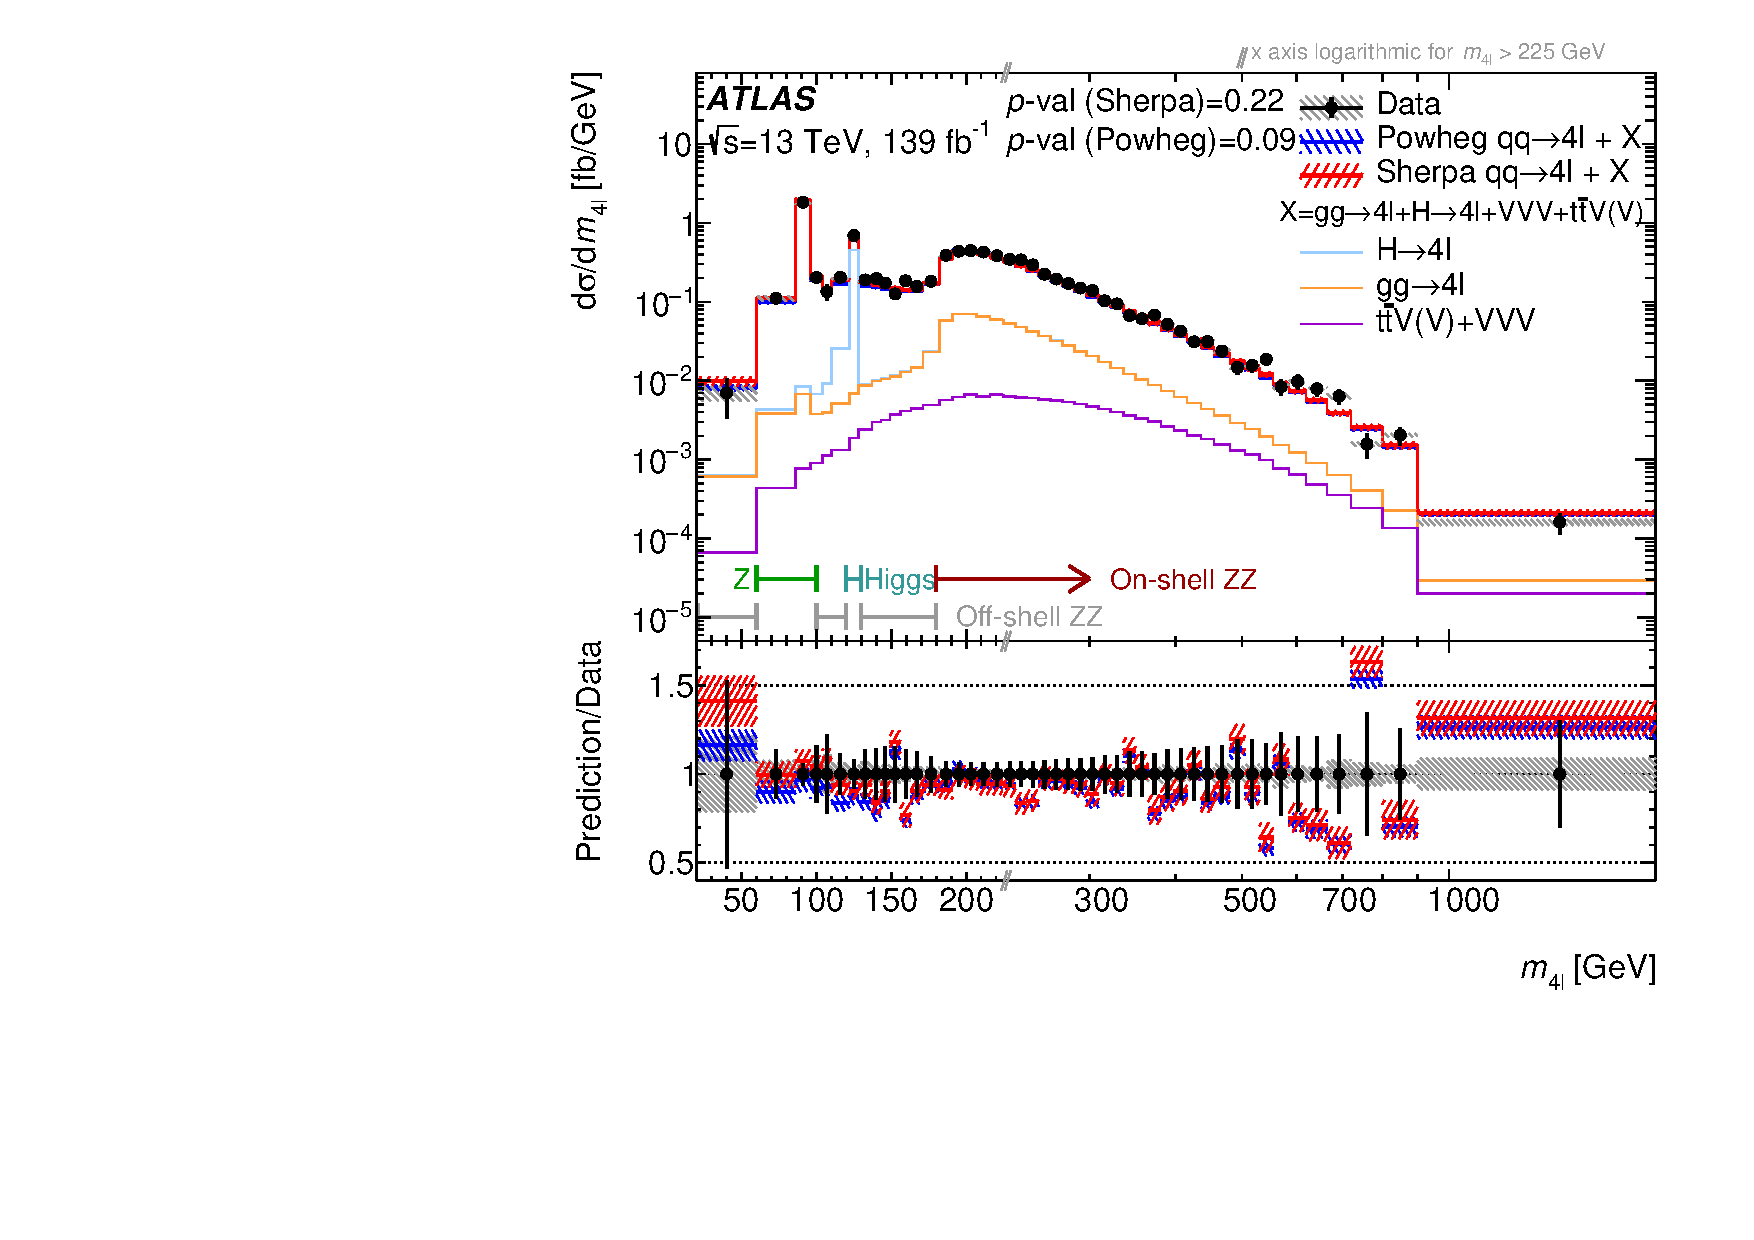
\includegraphics[width = 0.85\textwidth]{Figures/m4l/UnfoldedResults/linlog_Unfolded_Data_inclm4l.pdf} 
    \caption{Differential cross-section as a function of \mFourL. The measured data
  (black points)  are compared with the SM
  prediction using either \SHERPA{} (red, with red hashed
  band for the uncertainty) or \POWHEG{} + \pythia{} (blue,
  with blue hashed band for the uncertainty) to model the \qqFourL{} contribution. The error bars on the data points give the total uncertainty
  and the grey hashed band gives the systematic uncertainty. The
  breakdown of the contribution from different SM processes is also
  shown in successive stacked histograms.
  The short vertical lines terminating horizontal lines indicate the boundaries of the different
  \mFourL{} regions in which the other variables are measured.
  \Pvalue{}
  The
  lower panel shows the ratio of the SM predictions to the 
  data. The $x$-axis is on a linear scale until $\mFourL = 216$~\GeV,
  where it switches to a logarithmic scale. \label{fig:cross-sec-m4l}}
\end{figure}
In order to study the different \mFourL{} regions in more detail,  Figures~\ref{fig:mz1res} and~\ref{fig:mz2res} 
show the cross-section versus 
\mZOne{} and \mZTwo{} respectively in each region.
In the \HFourL{} region the contribution from Higgs production is
shown separately.

%% m4l vs pt4l
\begin{figure}[htb!]
    \begin{subfigure}{.49\textwidth}\centering
      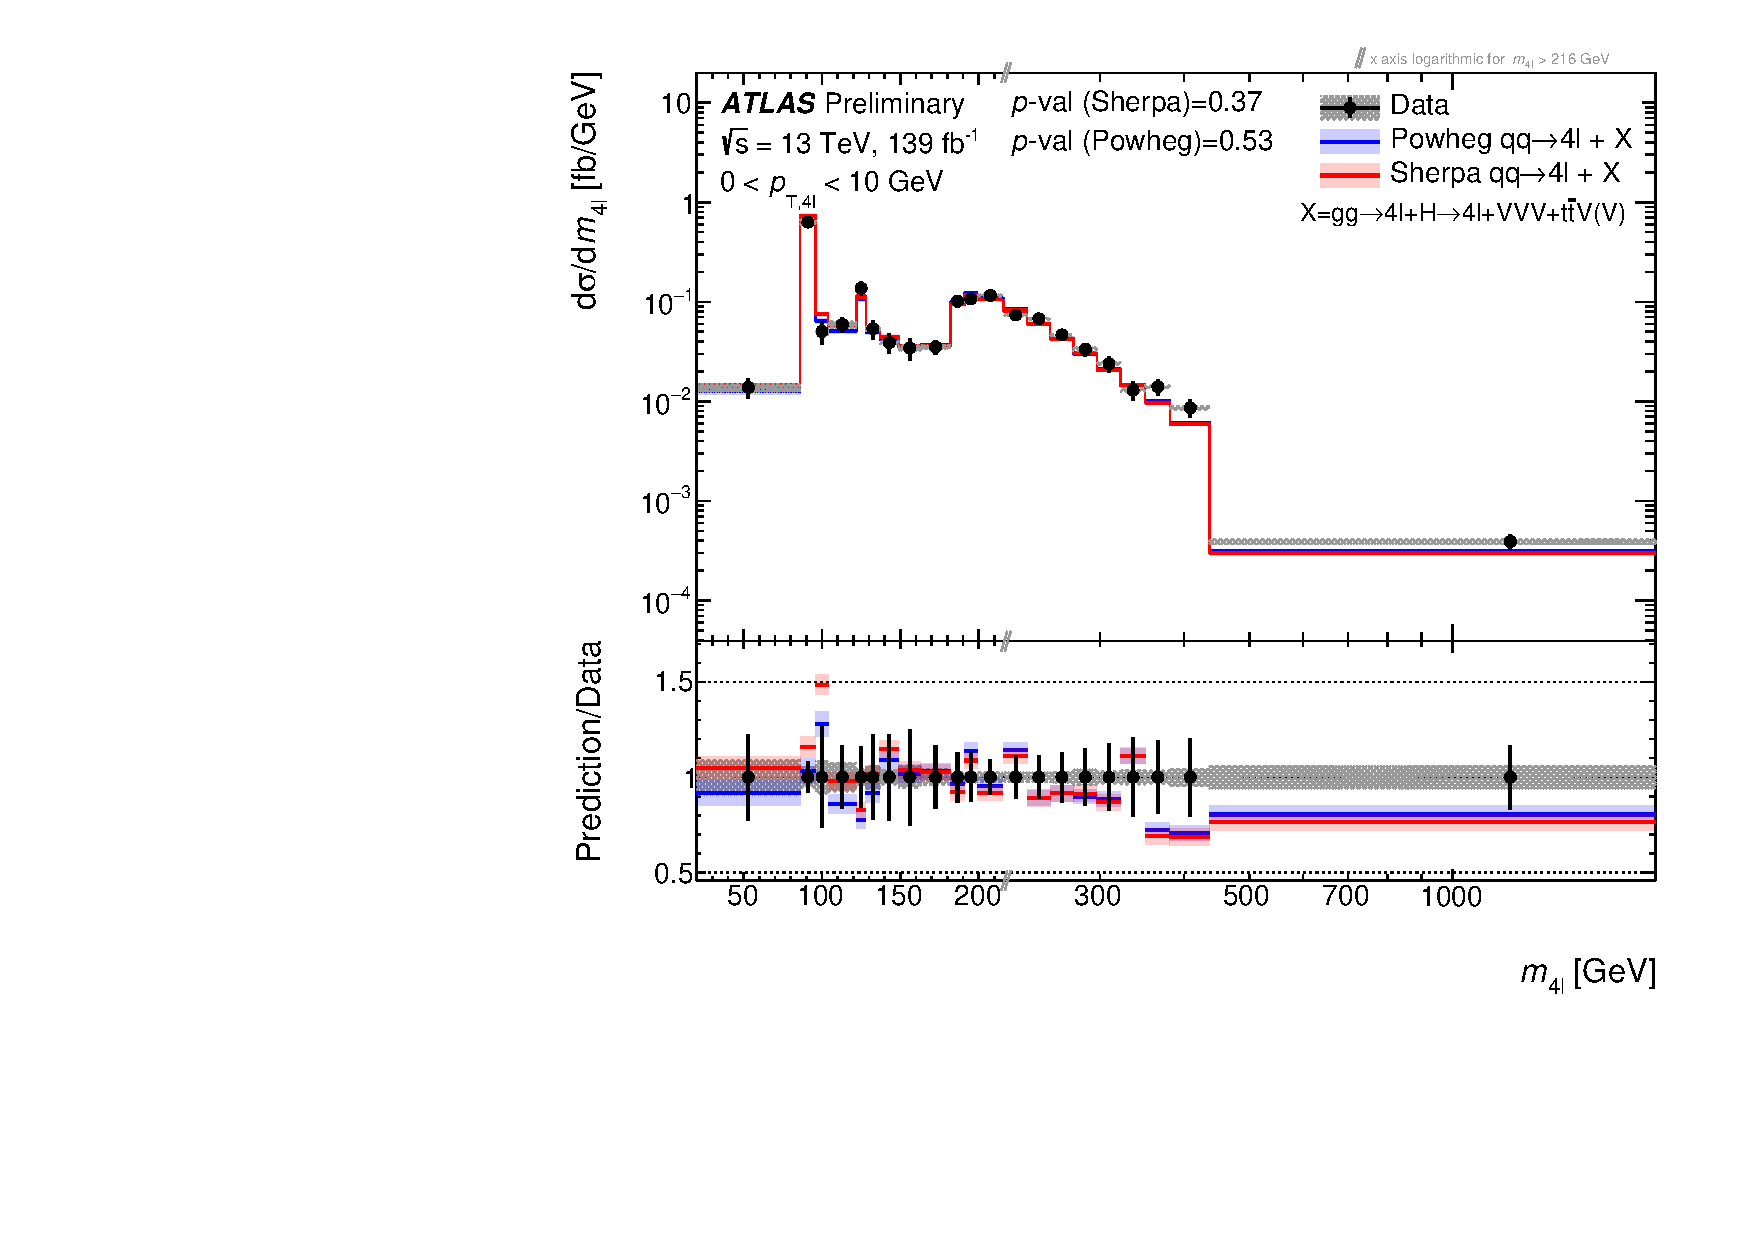
\includegraphics[width=.99\linewidth]{Figures/m4l/UnfoldedResults/linlog_Unfolded_Data_m4l_pt4l0-10.pdf}\caption{$\unit{0}{\GeV} <  \ptFourL  < \unit{10}{\GeV}$}\label{fig:sub-first}
    \end{subfigure}
    \begin{subfigure}{.49\textwidth}\centering
      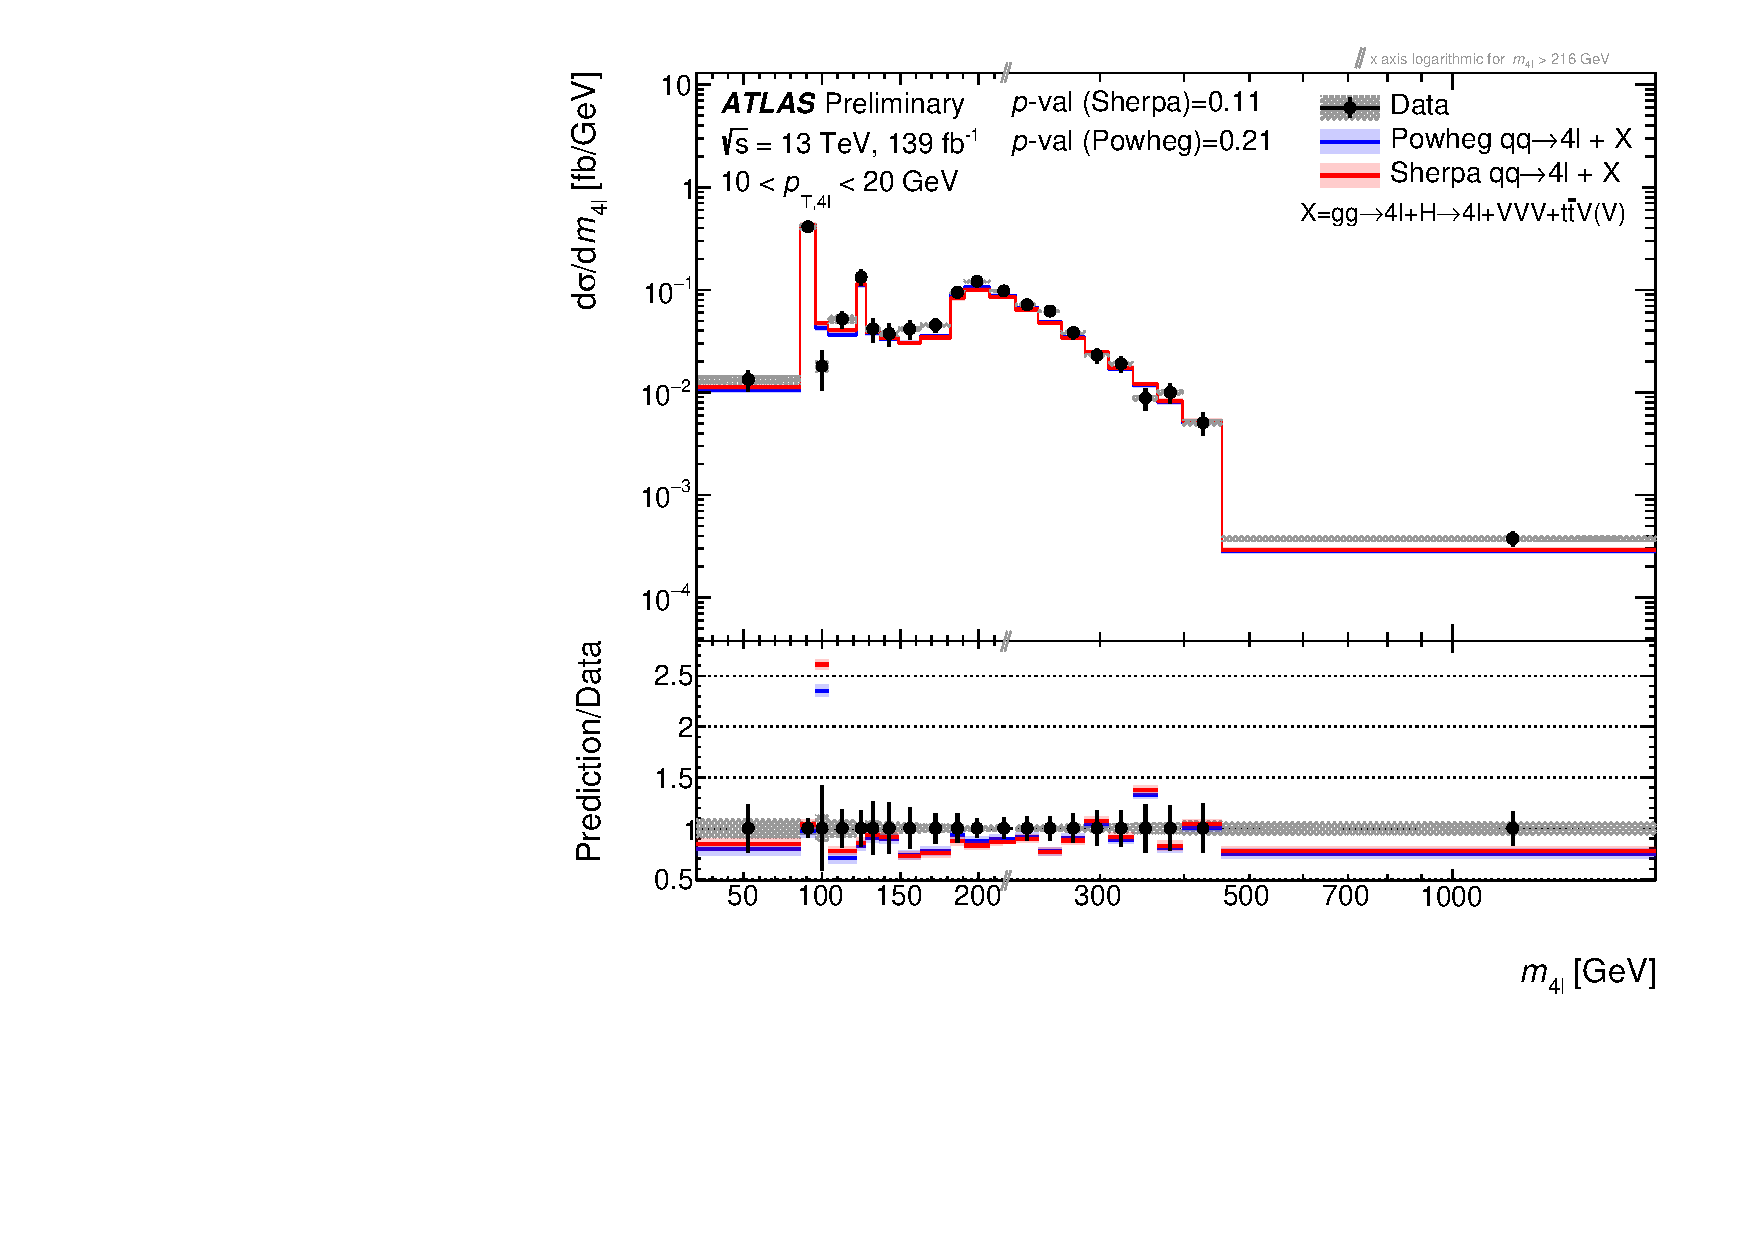
\includegraphics[width=.99\linewidth]{Figures/m4l/UnfoldedResults/linlog_Unfolded_Data_m4l_pt4l10-20.pdf} \caption{$\unit{10}{\GeV} <  \ptFourL  < \unit{20}{\GeV}$}\label{fig:sub-second}
    \end{subfigure}
    \begin{subfigure}{.49\textwidth}\centering
      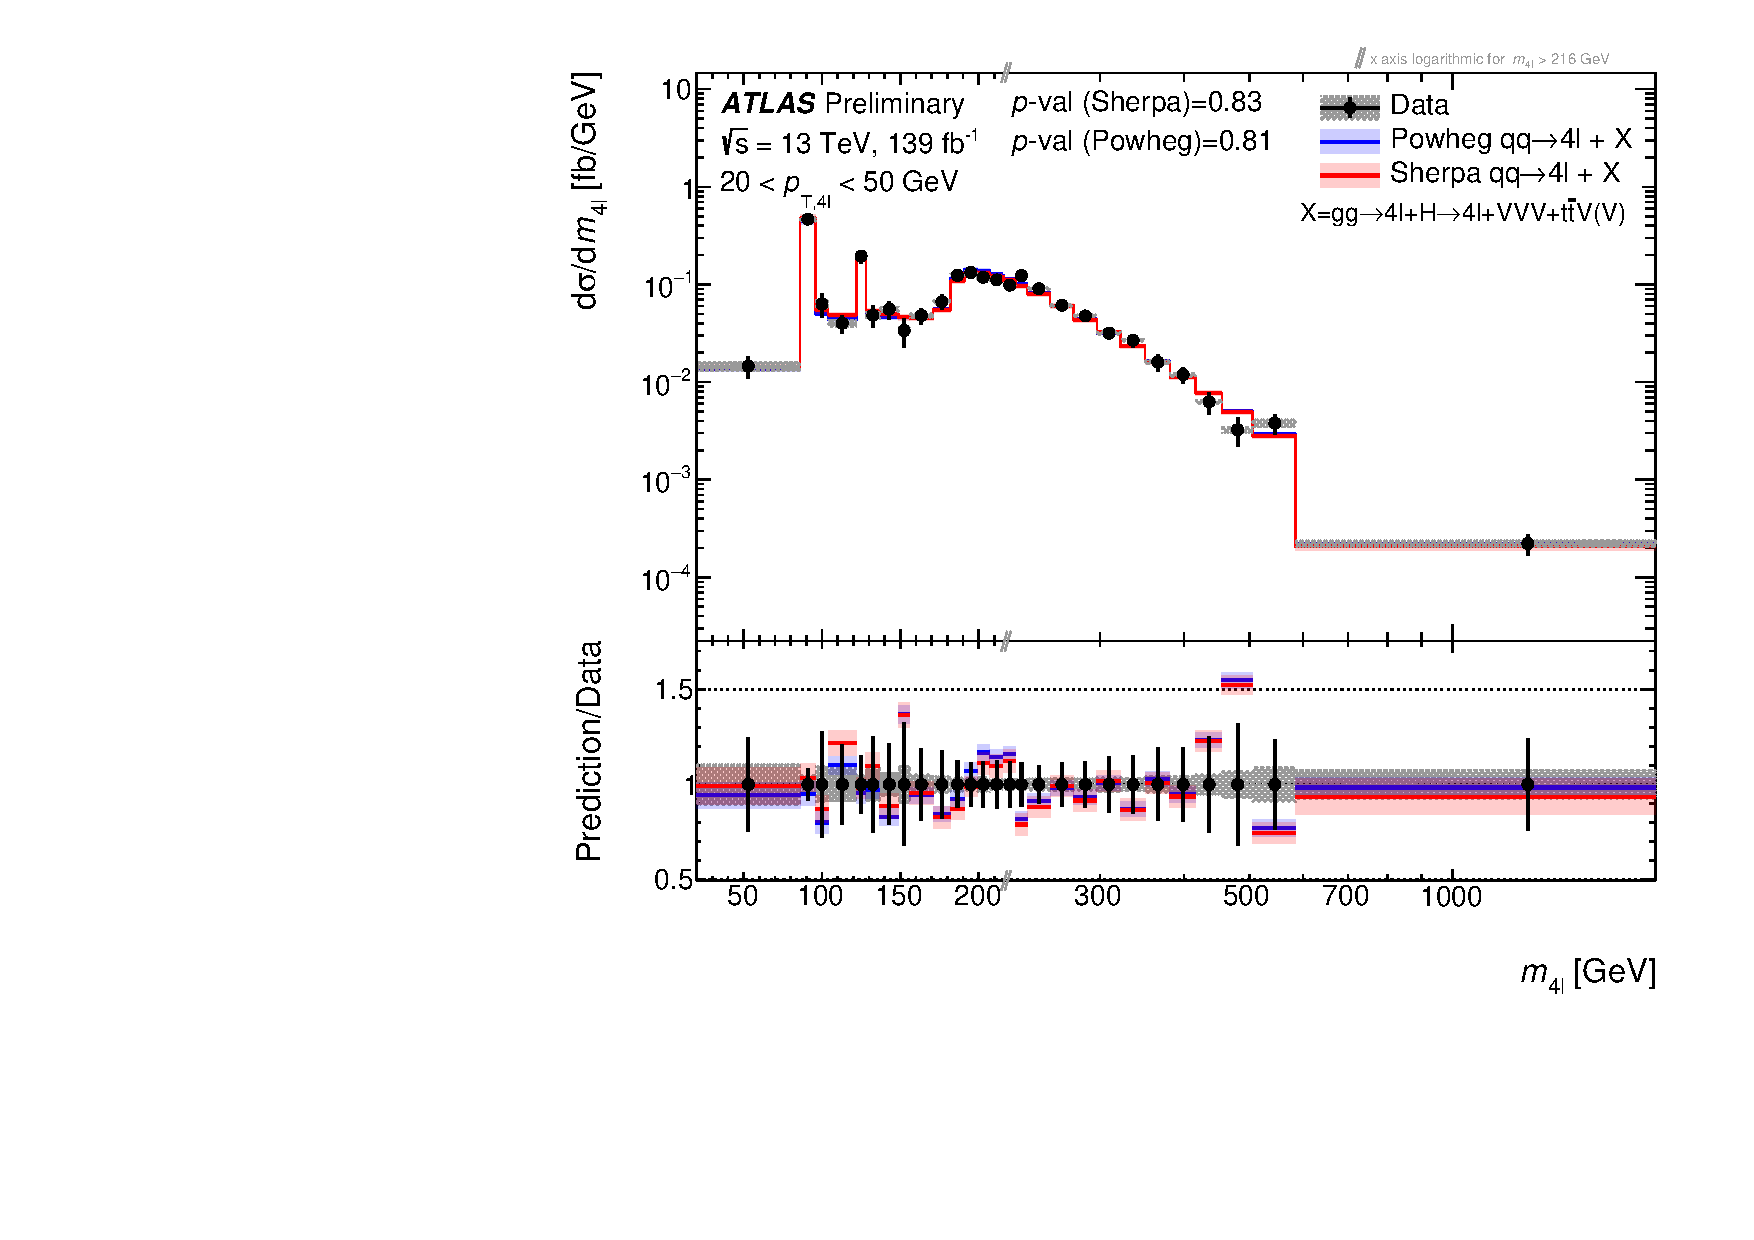
\includegraphics[width=.99\linewidth]{Figures/m4l/UnfoldedResults/linlog_Unfolded_Data_m4l_pt4l20-50.pdf}  \caption{$\unit{20}{\GeV} <  \ptFourL  < \unit{50}{\GeV}$}\label{fig:sub-third}
    \end{subfigure}
    \begin{subfigure}{.49\textwidth}\centering
      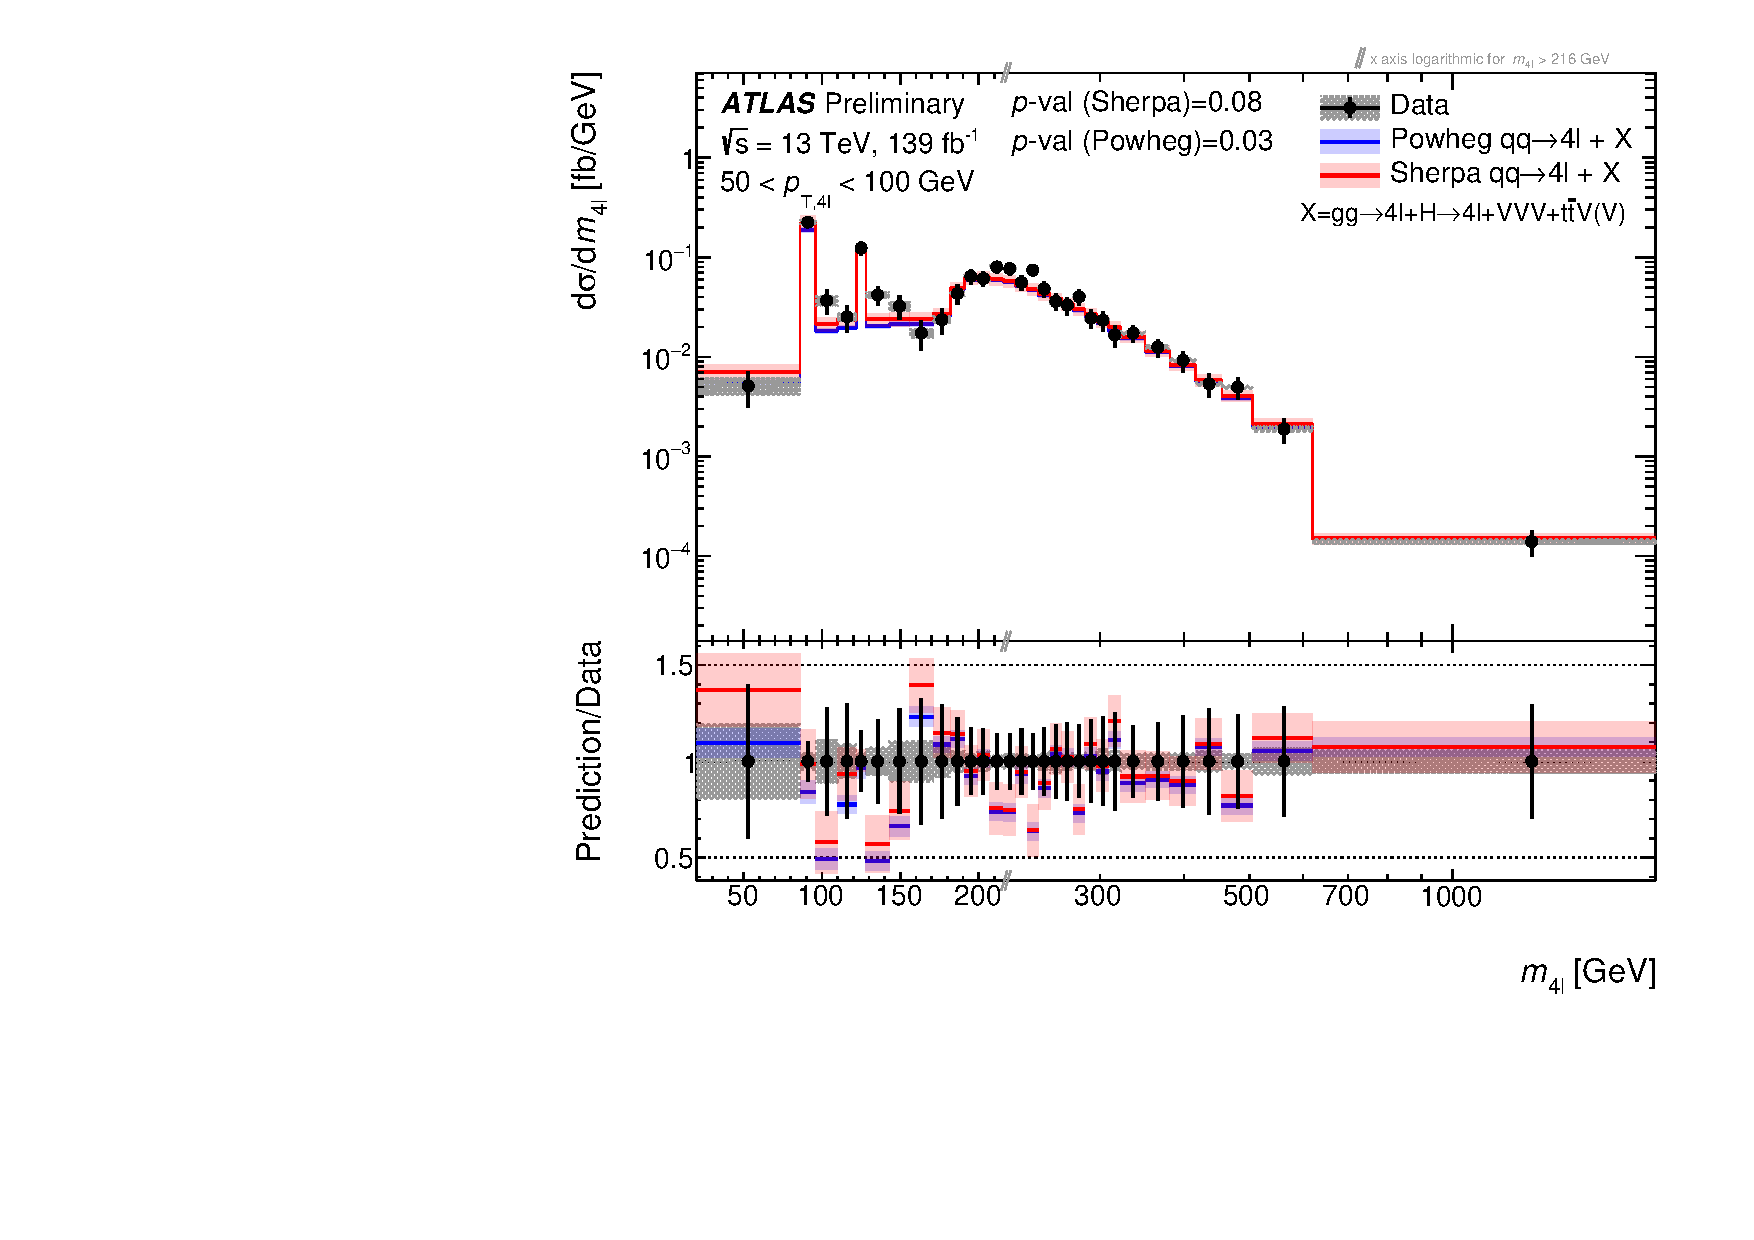
\includegraphics[width=.99\linewidth]{Figures/m4l/UnfoldedResults/linlog_Unfolded_Data_m4l_pt4l50-100.pdf}  \caption{$\unit{50}{\GeV} <  \ptFourL  < \unit{100}{\GeV}$}\label{fig:sub-fourth}
    \end{subfigure}
        \begin{subfigure}{.49\textwidth}\centering
      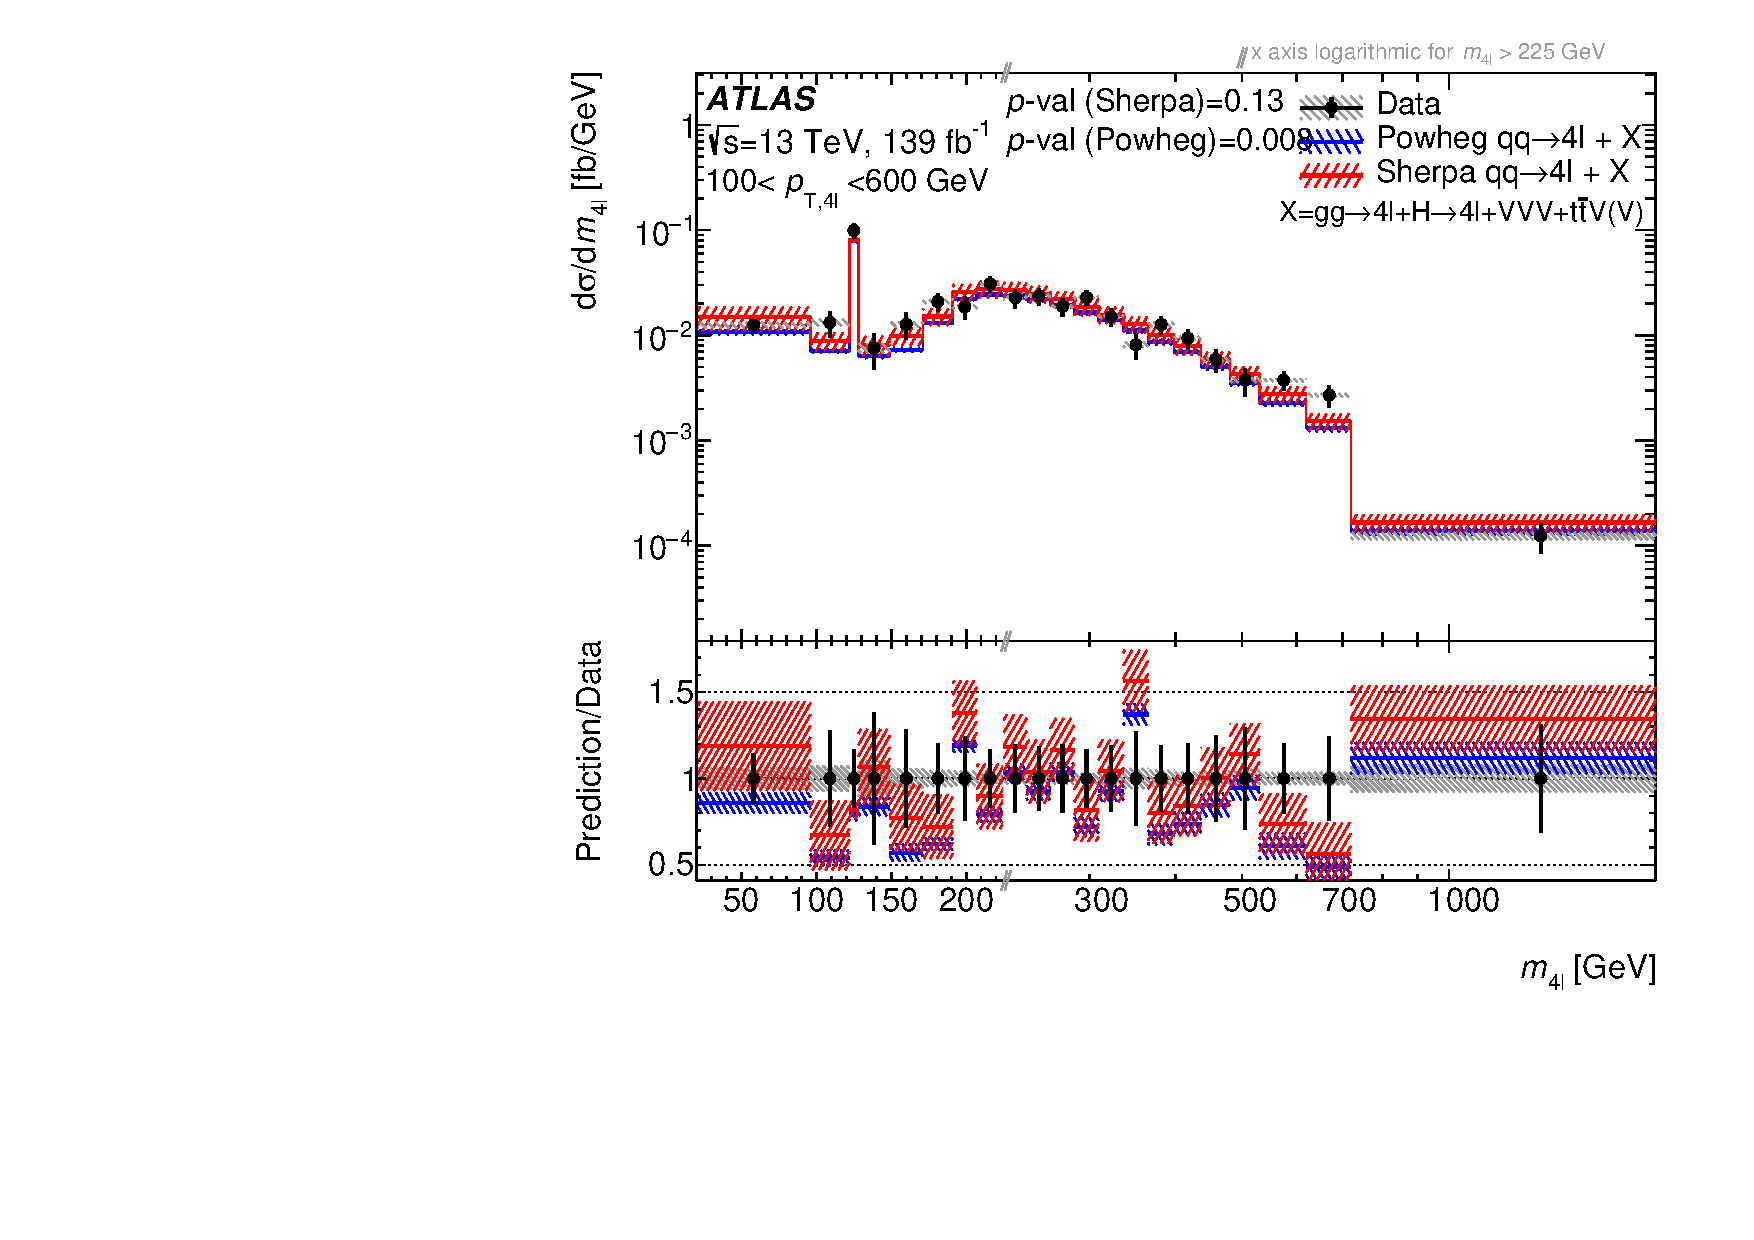
\includegraphics[width=.99\linewidth]{Figures/m4l/UnfoldedResults/linlog_Unfolded_Data_m4l_pt4l100-600.pdf}  \caption{$\unit{100}{\GeV} <  \ptFourL  < \unit{60 0}{\GeV}$}\label{fig:sub-fifth}
    \end{subfigure}
    \caption{Differential cross-section as a function of \mFourL{} in slices of \ptFourL{}. The measured data (black points) are  compared with the SM prediction using either \SHERPA{} (red, with red hashed band for the uncertainty) or \POWHEG{} + \pythia{} (blue, with blue hashed band for the uncertainty) to model the \qqFourL{} contribution. The error bars on the data points give the total uncertainty and the grey hashed band gives the systematic uncertainty. \Pvalue{} The  lower panel shows the ratio of the SM predictions to the data.}
    \label{fig:m4l_pt4l}
\end{figure}

%% m4l vs y4l
\begin{figure}[htb!]
    \begin{subfigure}{.49\textwidth}\centering
      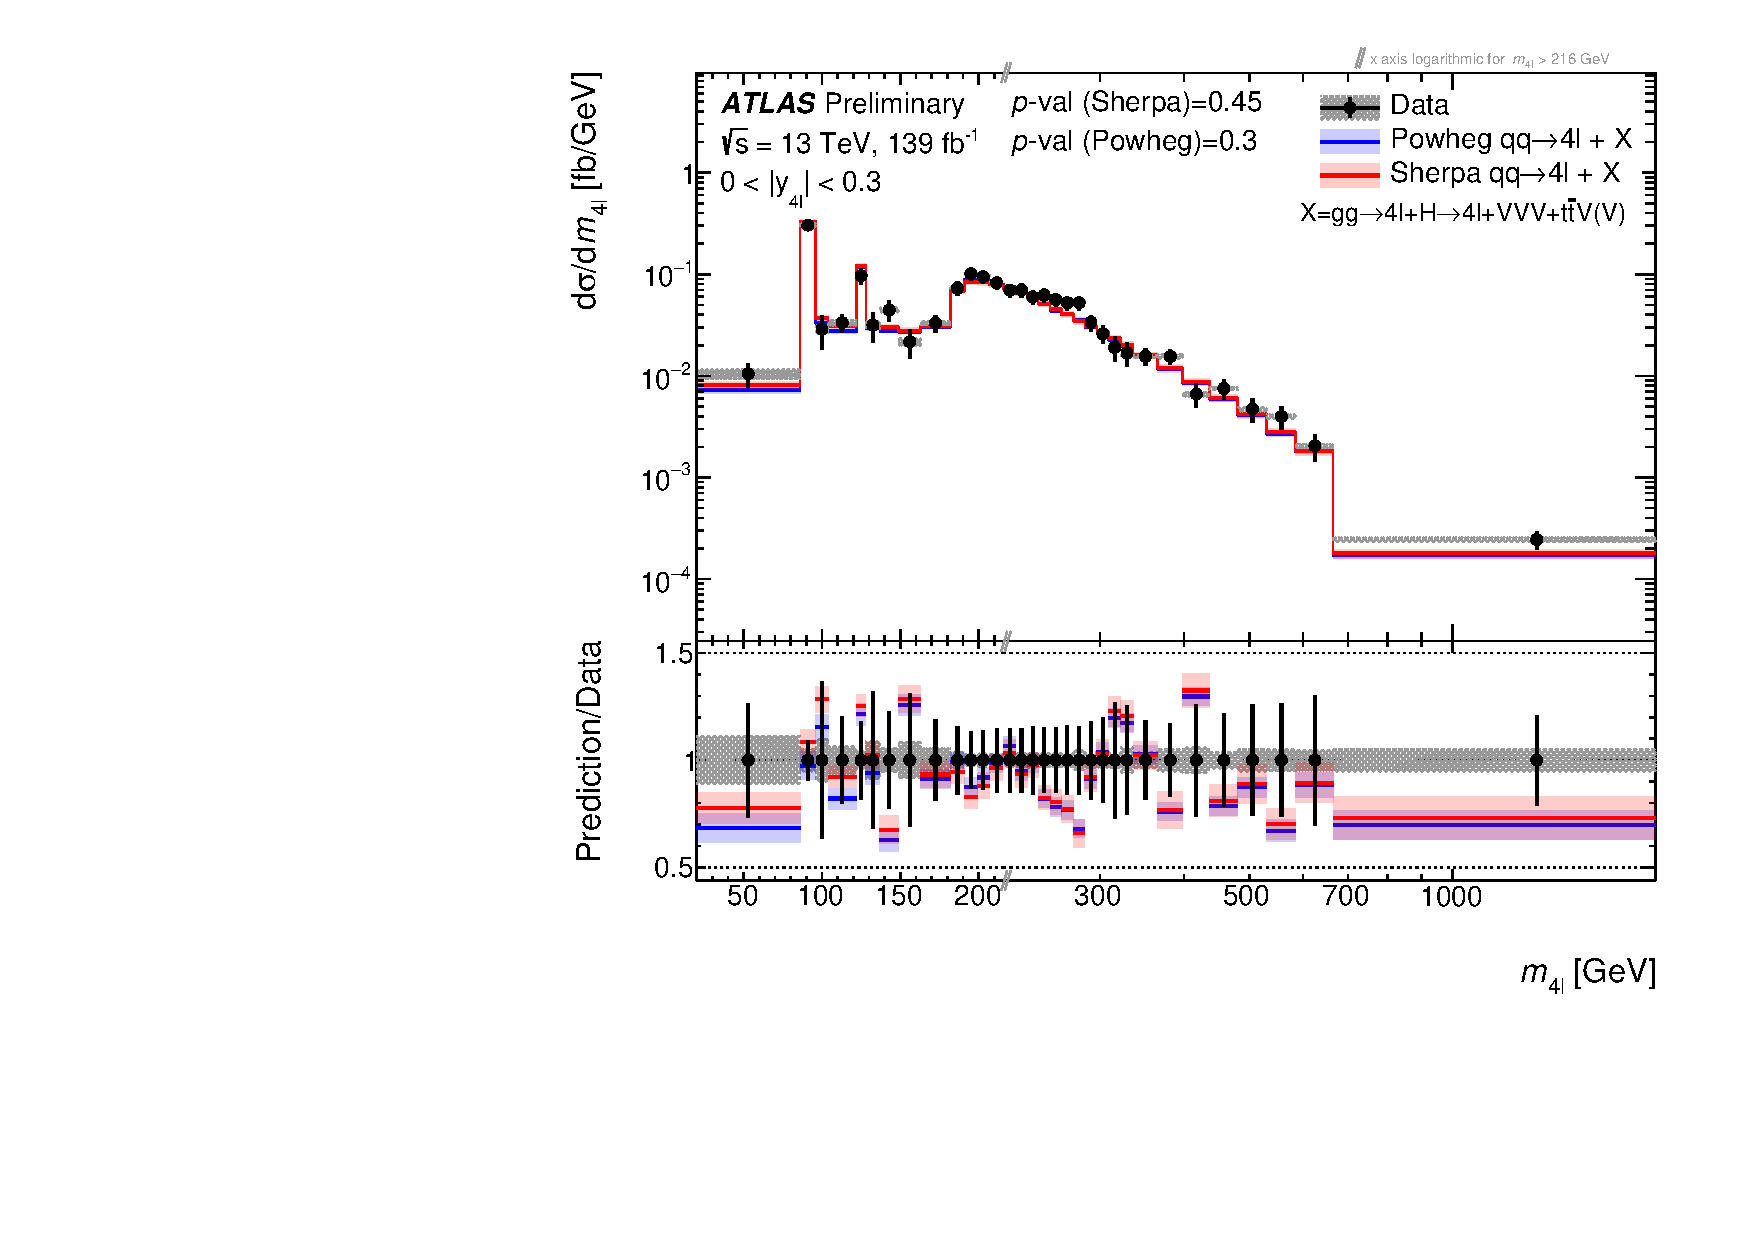
\includegraphics[width=.99\linewidth]{Figures/m4l/UnfoldedResults/linlog_Unfolded_Data_m4l_y4l0-0dot3.pdf}\caption{0 < \yFourL{} < 0.3}\label{fig:sub-first}
    \end{subfigure}
    \begin{subfigure}{.49\textwidth}\centering
      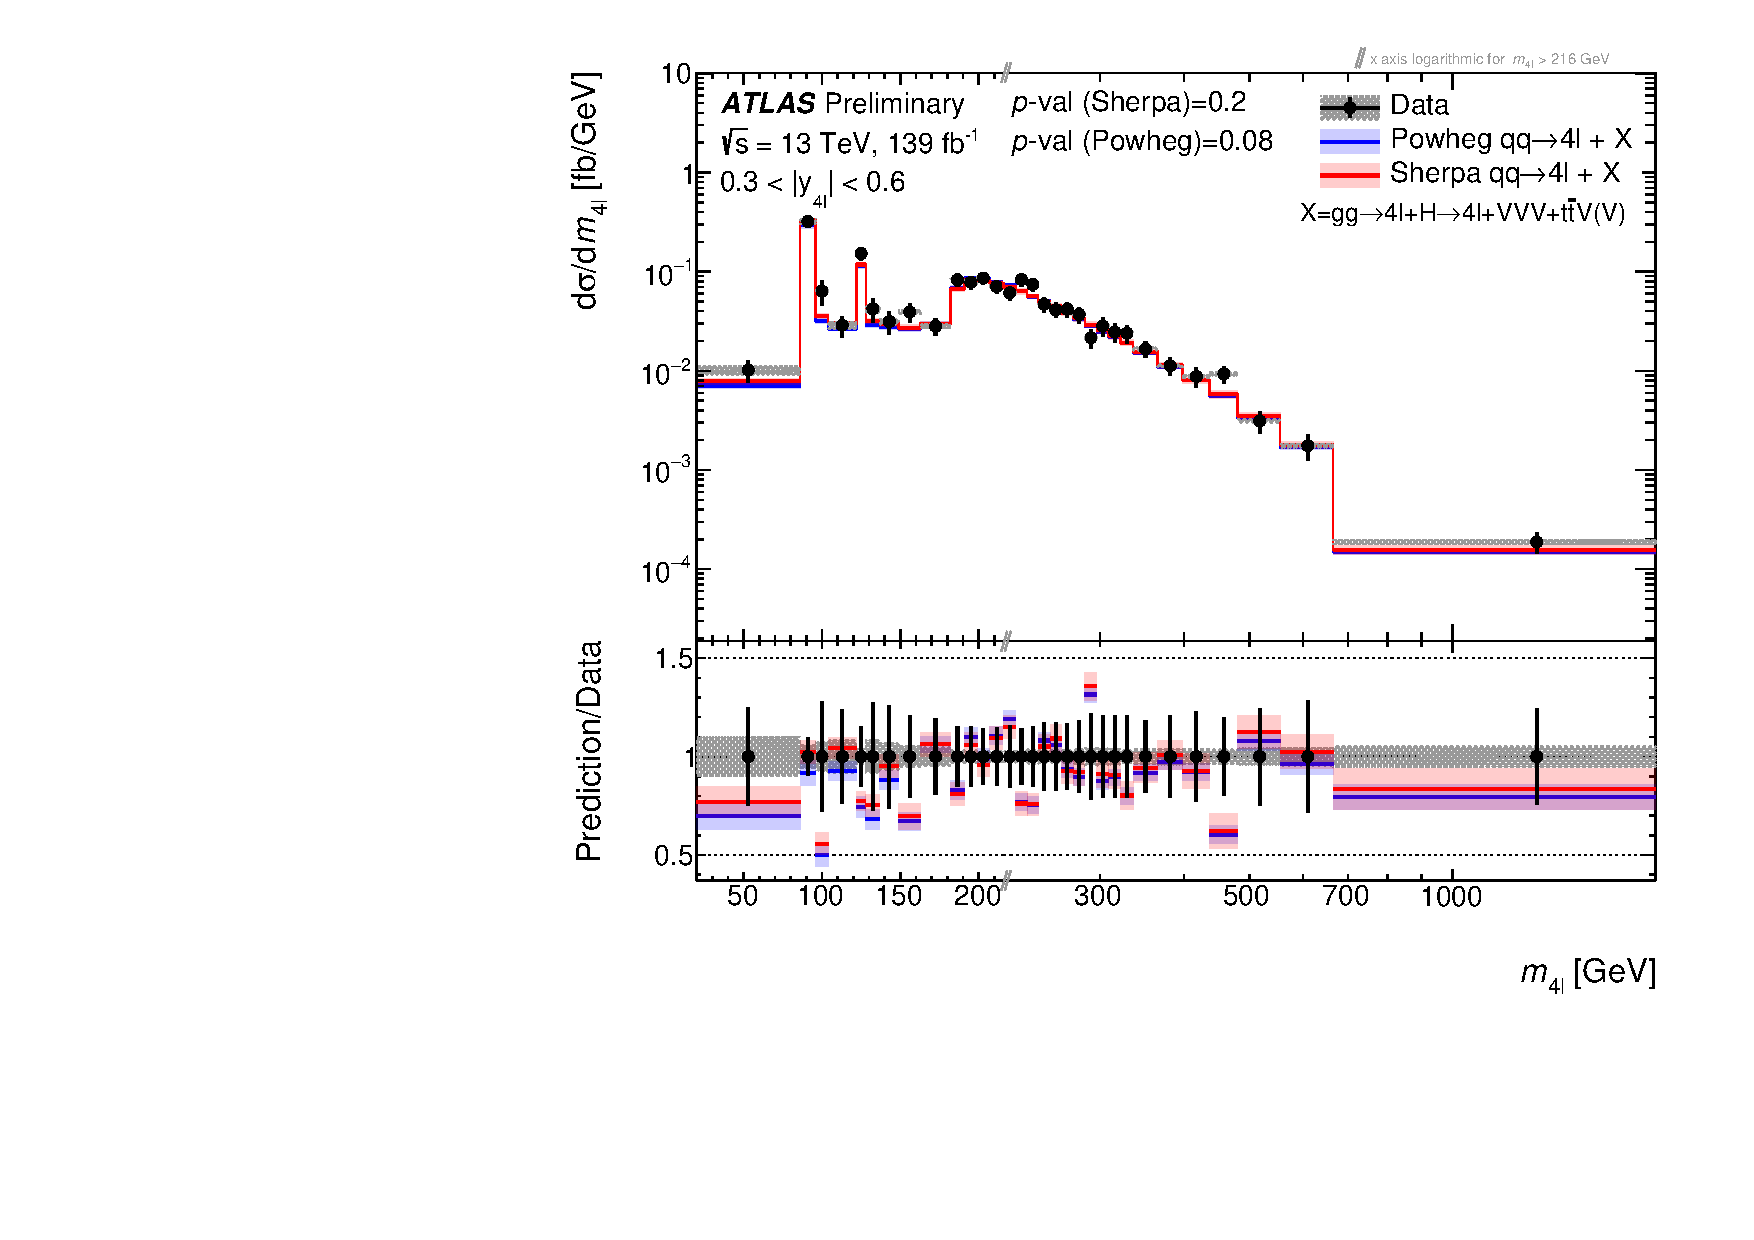
\includegraphics[width=.99\linewidth]{Figures/m4l/UnfoldedResults/linlog_Unfolded_Data_m4l_y4l0dot3-0dot6.pdf} \caption{0.3 < \yFourL{} < 0.6}\label{fig:sub-second}
    \end{subfigure}
    \begin{subfigure}{.49\textwidth}\centering
      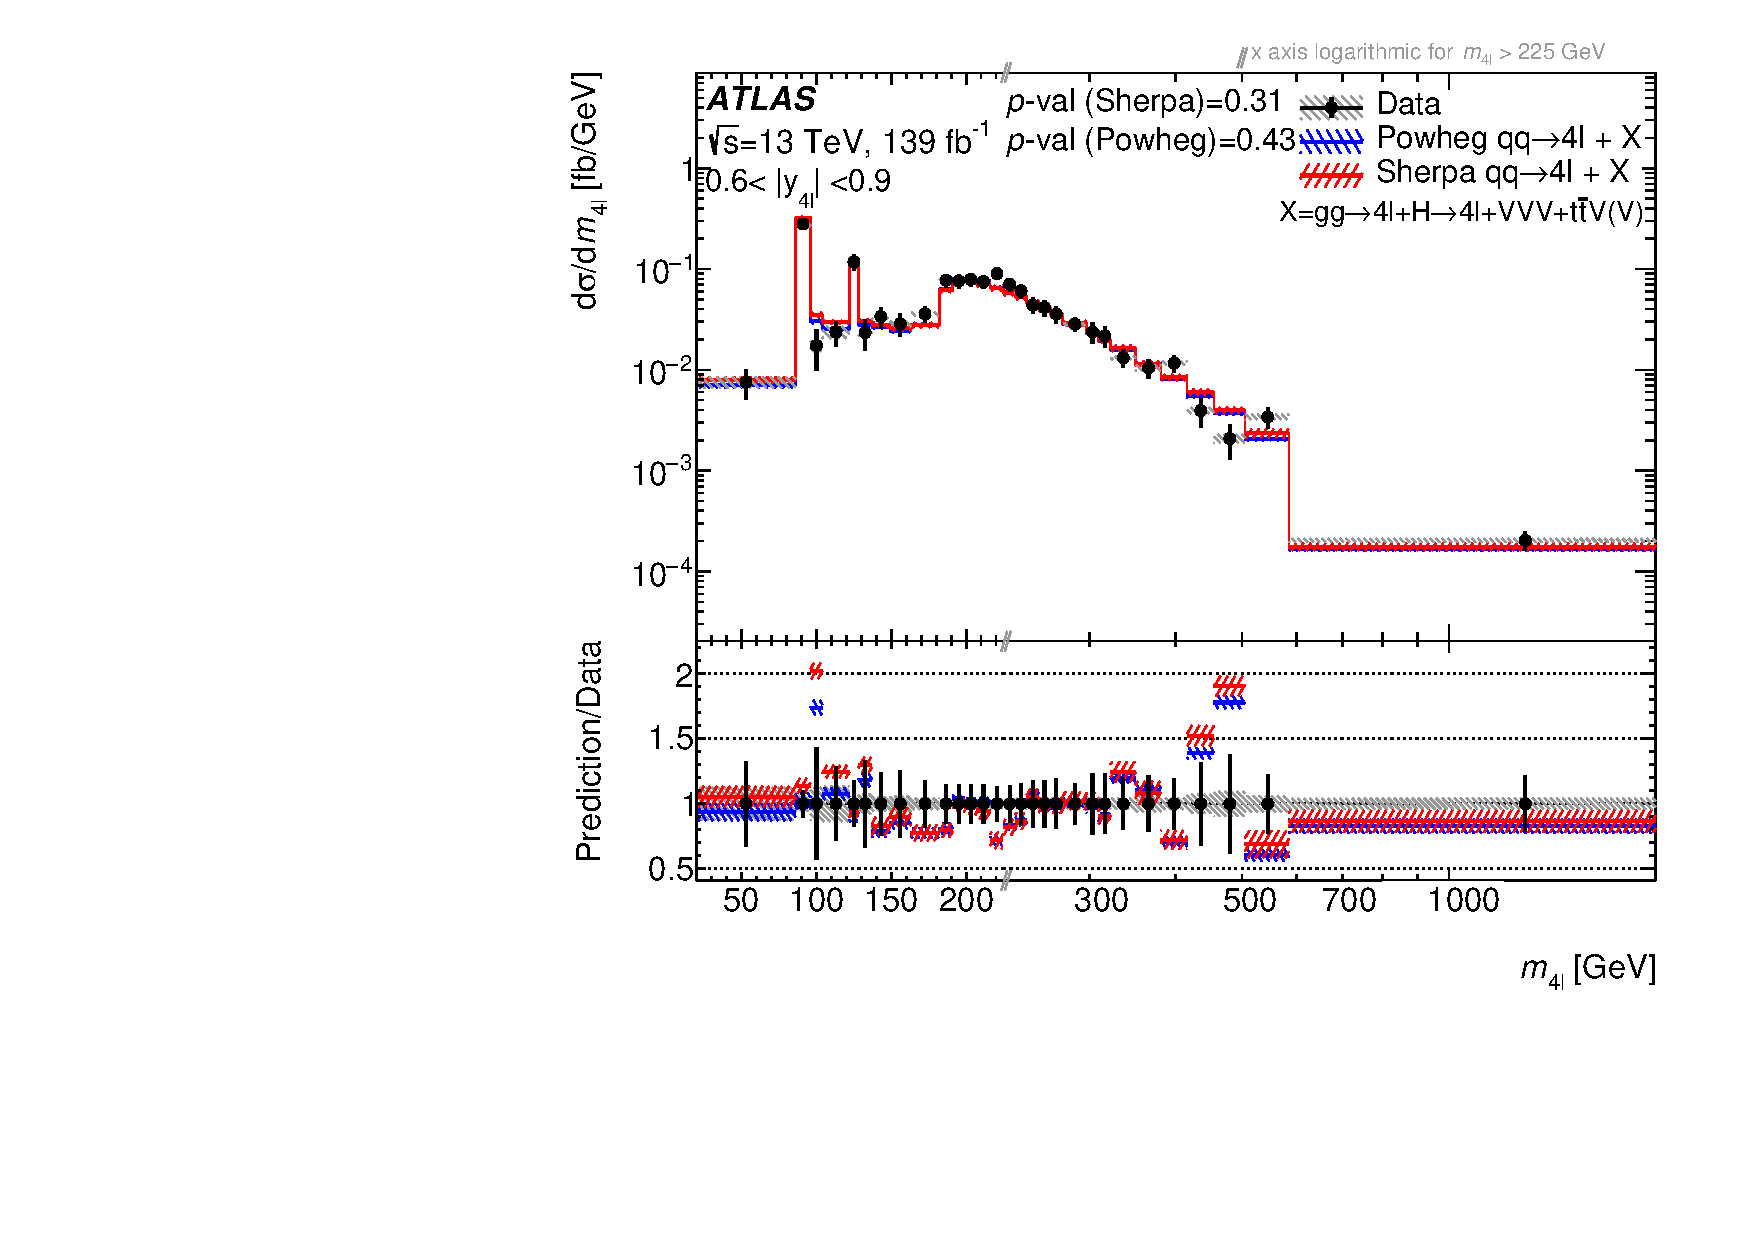
\includegraphics[width=.99\linewidth]{Figures/m4l/UnfoldedResults/linlog_Unfolded_Data_m4l_y4l0dot6-0dot9.pdf}  \caption{0.6 < \yFourL{} < 0.9}\label{fig:sub-third}
    \end{subfigure}
    \begin{subfigure}{.49\textwidth}\centering
      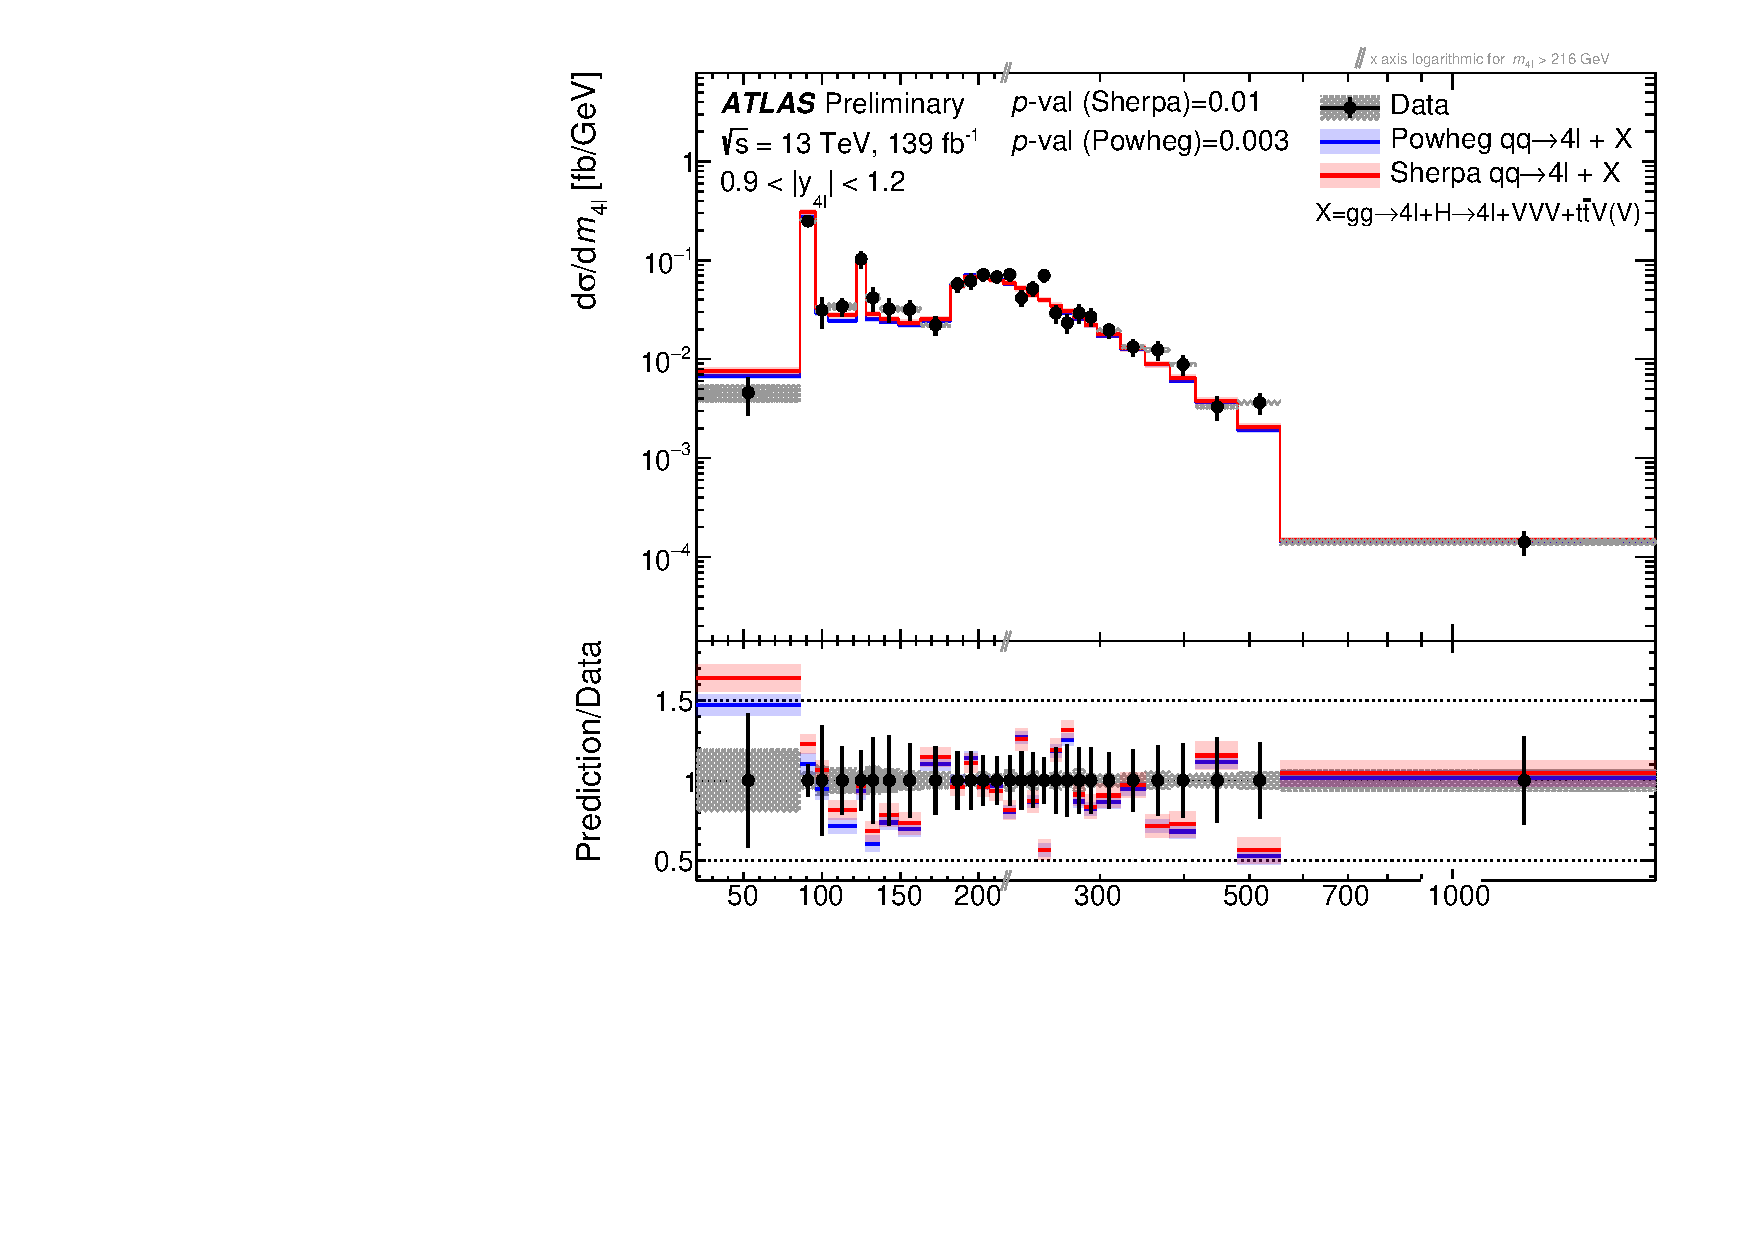
\includegraphics[width=.99\linewidth]{Figures/m4l/UnfoldedResults/linlog_Unfolded_Data_m4l_y4l0dot9-1dot2.pdf}  \caption{0.9 < \yFourL{} < 1.2}\label{fig:sub-fourth}
    \end{subfigure}
        \begin{subfigure}{.49\textwidth}\centering
      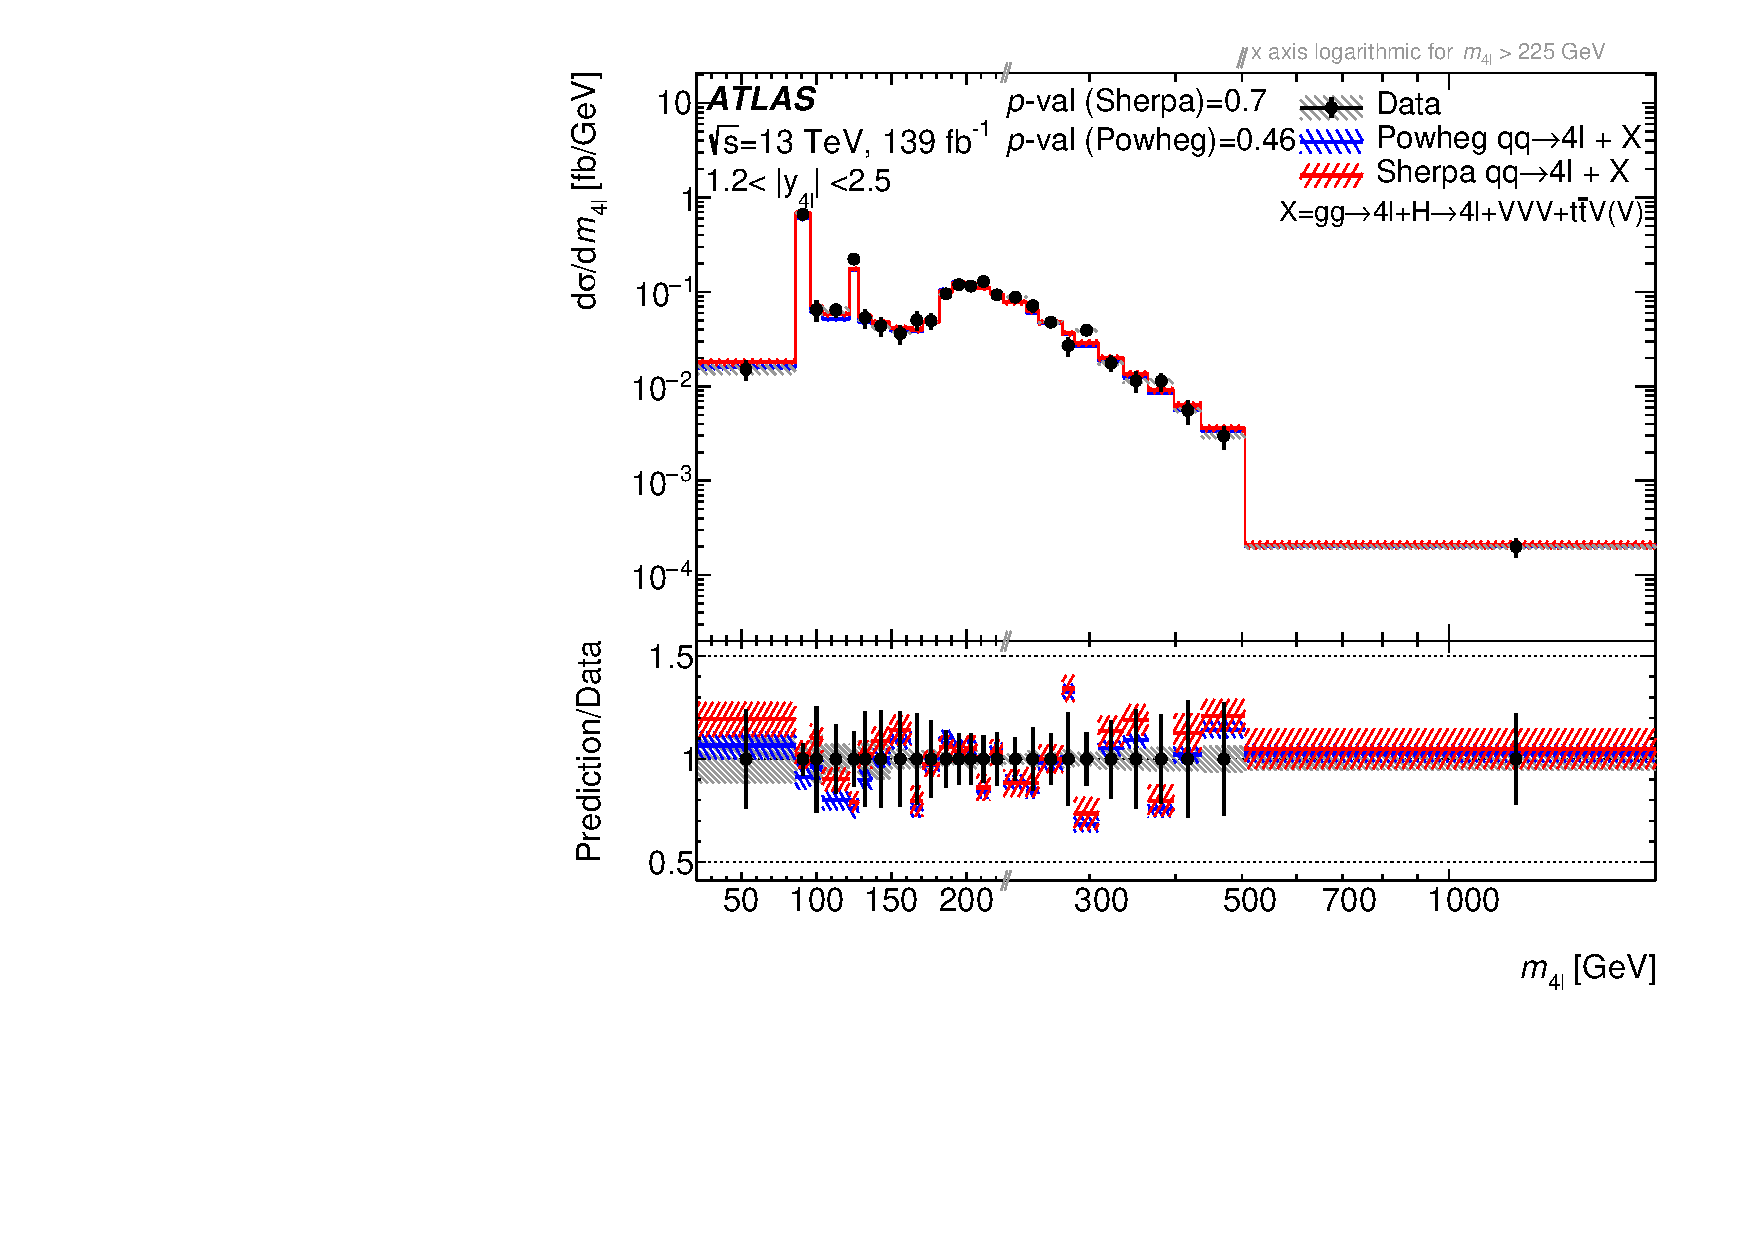
\includegraphics[width=.99\linewidth]{Figures/m4l/UnfoldedResults/linlog_Unfolded_Data_m4l_y4l1dot2-2dot5.pdf}  \caption{1.2 < \yFourL{} < 2.5}\label{fig:sub-fifth}
    \end{subfigure}
    \caption{Differential cross-section as a function of \mFourL{} in slices of \yFourL{}. The measured data (black points) are  compared with the SM prediction using either \SHERPA{} (red, with red hashed band for the uncertainty) or \POWHEG{} + \pythia{} (blue, with blue hashed band for the uncertainty) to model the \qqFourL{} contribution. The error bars on the data points give the total uncertainty and the grey hashed band gives the systematic uncertainty. \Pvalue{} The  lower panel shows the ratio of the SM predictions to the data.}
    \label{fig:m4l_y4l}
\end{figure}

%% m4l vs flavour
\begin{figure}[htb!]
    \begin{subfigure}{.49\textwidth}\centering
      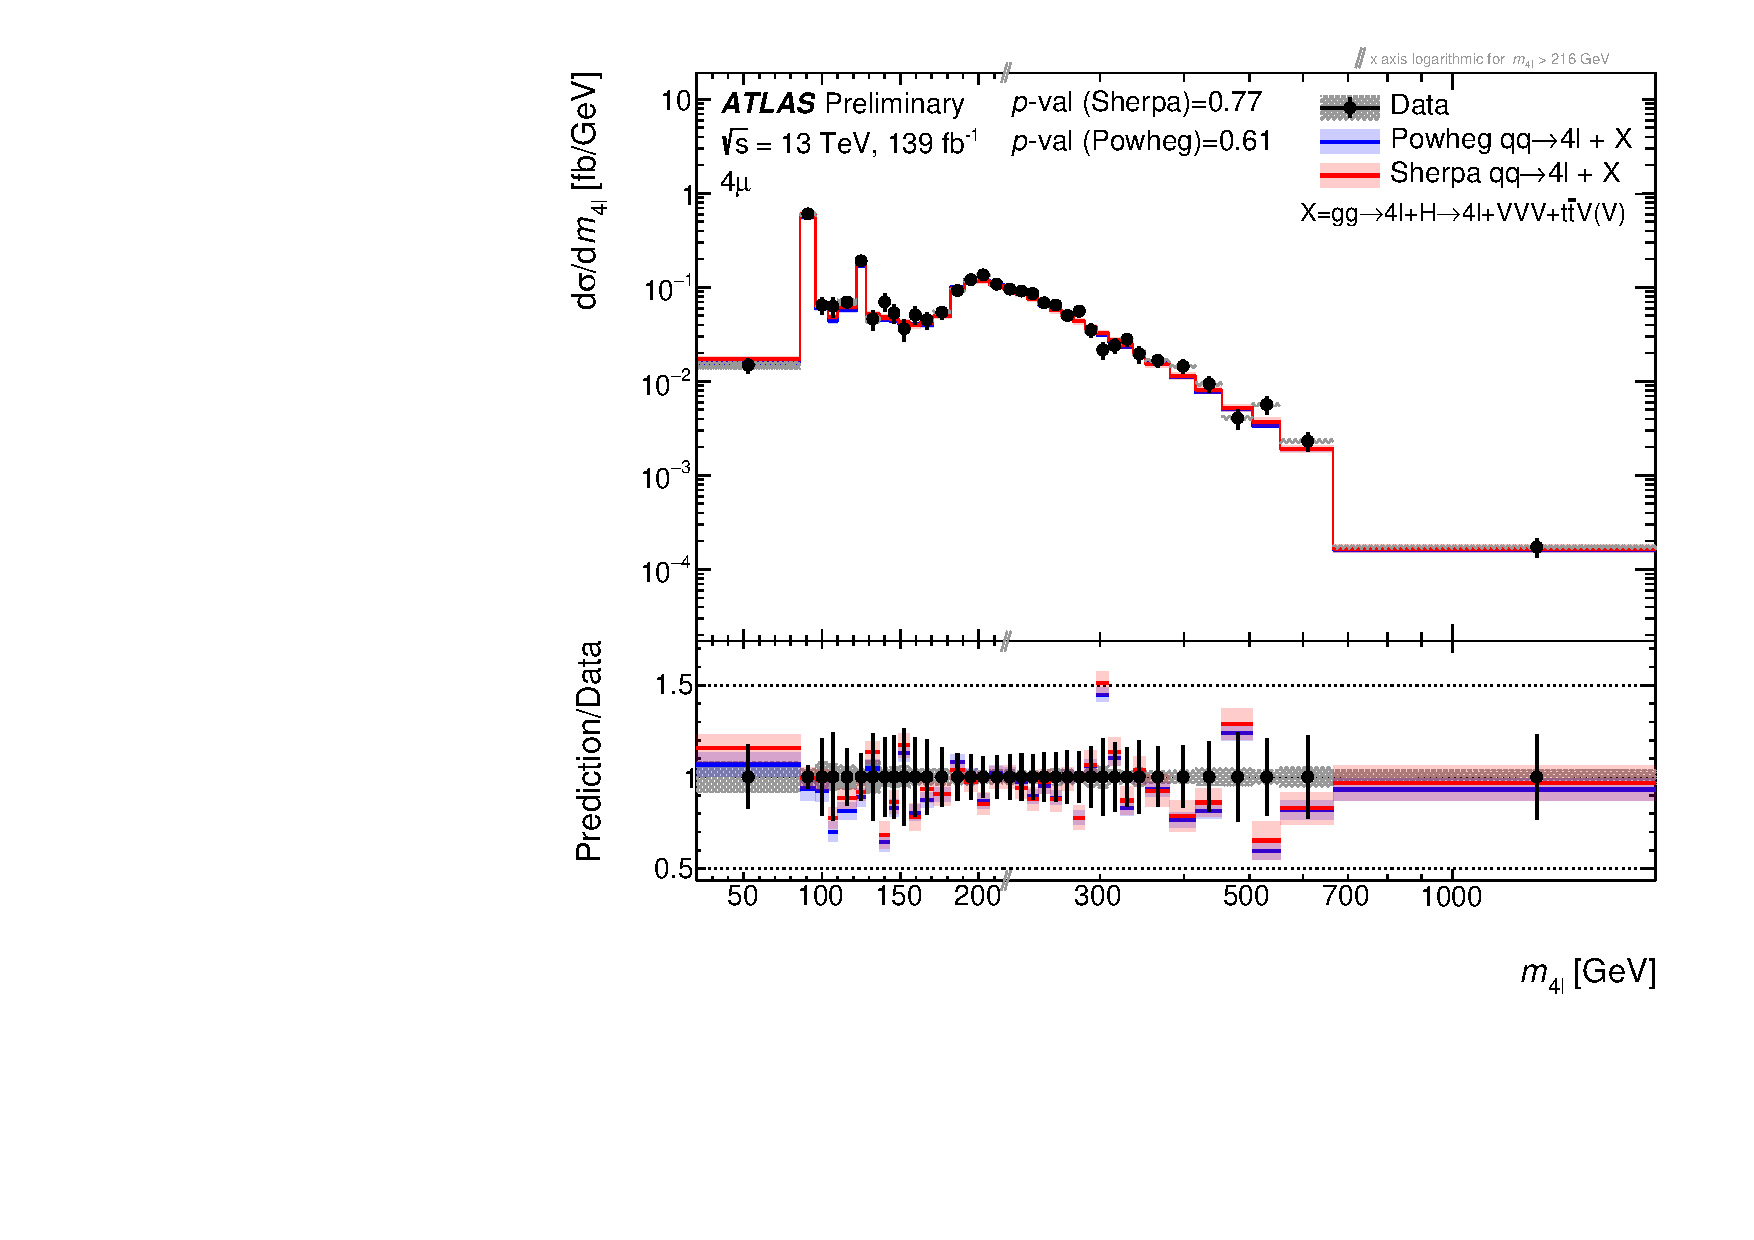
\includegraphics[width=.99\linewidth]{Figures/m4l/UnfoldedResults/linlog_Unfolded_Data_m4l_event_type4mu.pdf}\caption{$4\mu$ channel}\label{fig:sub-first}
    \end{subfigure}
    \begin{subfigure}{.49\textwidth}\centering
      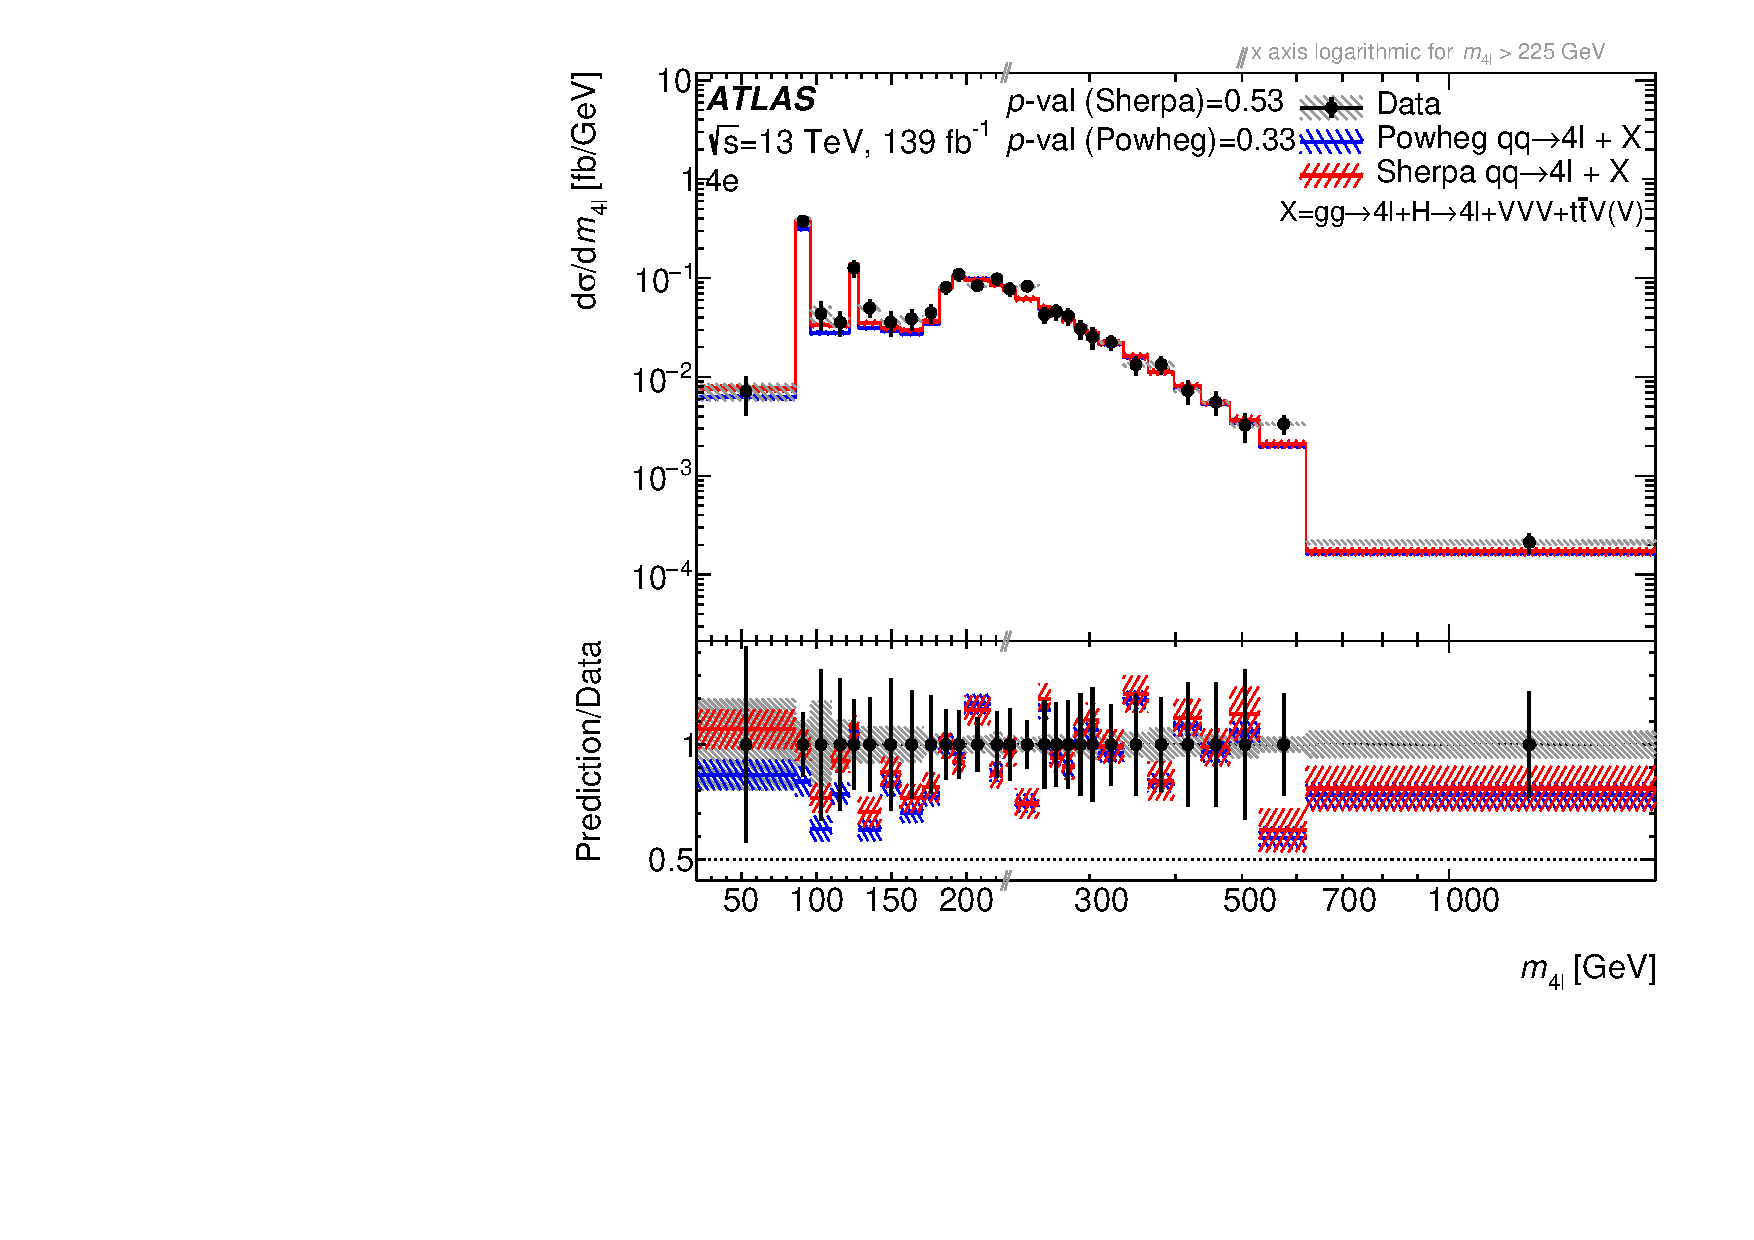
\includegraphics[width=.99\linewidth]{Figures/m4l/UnfoldedResults/linlog_Unfolded_Data_m4l_event_type4e.pdf} \caption{$4e$ channel}\label{fig:sub-second}
    \end{subfigure}
    \begin{subfigure}{.49\textwidth}\centering
      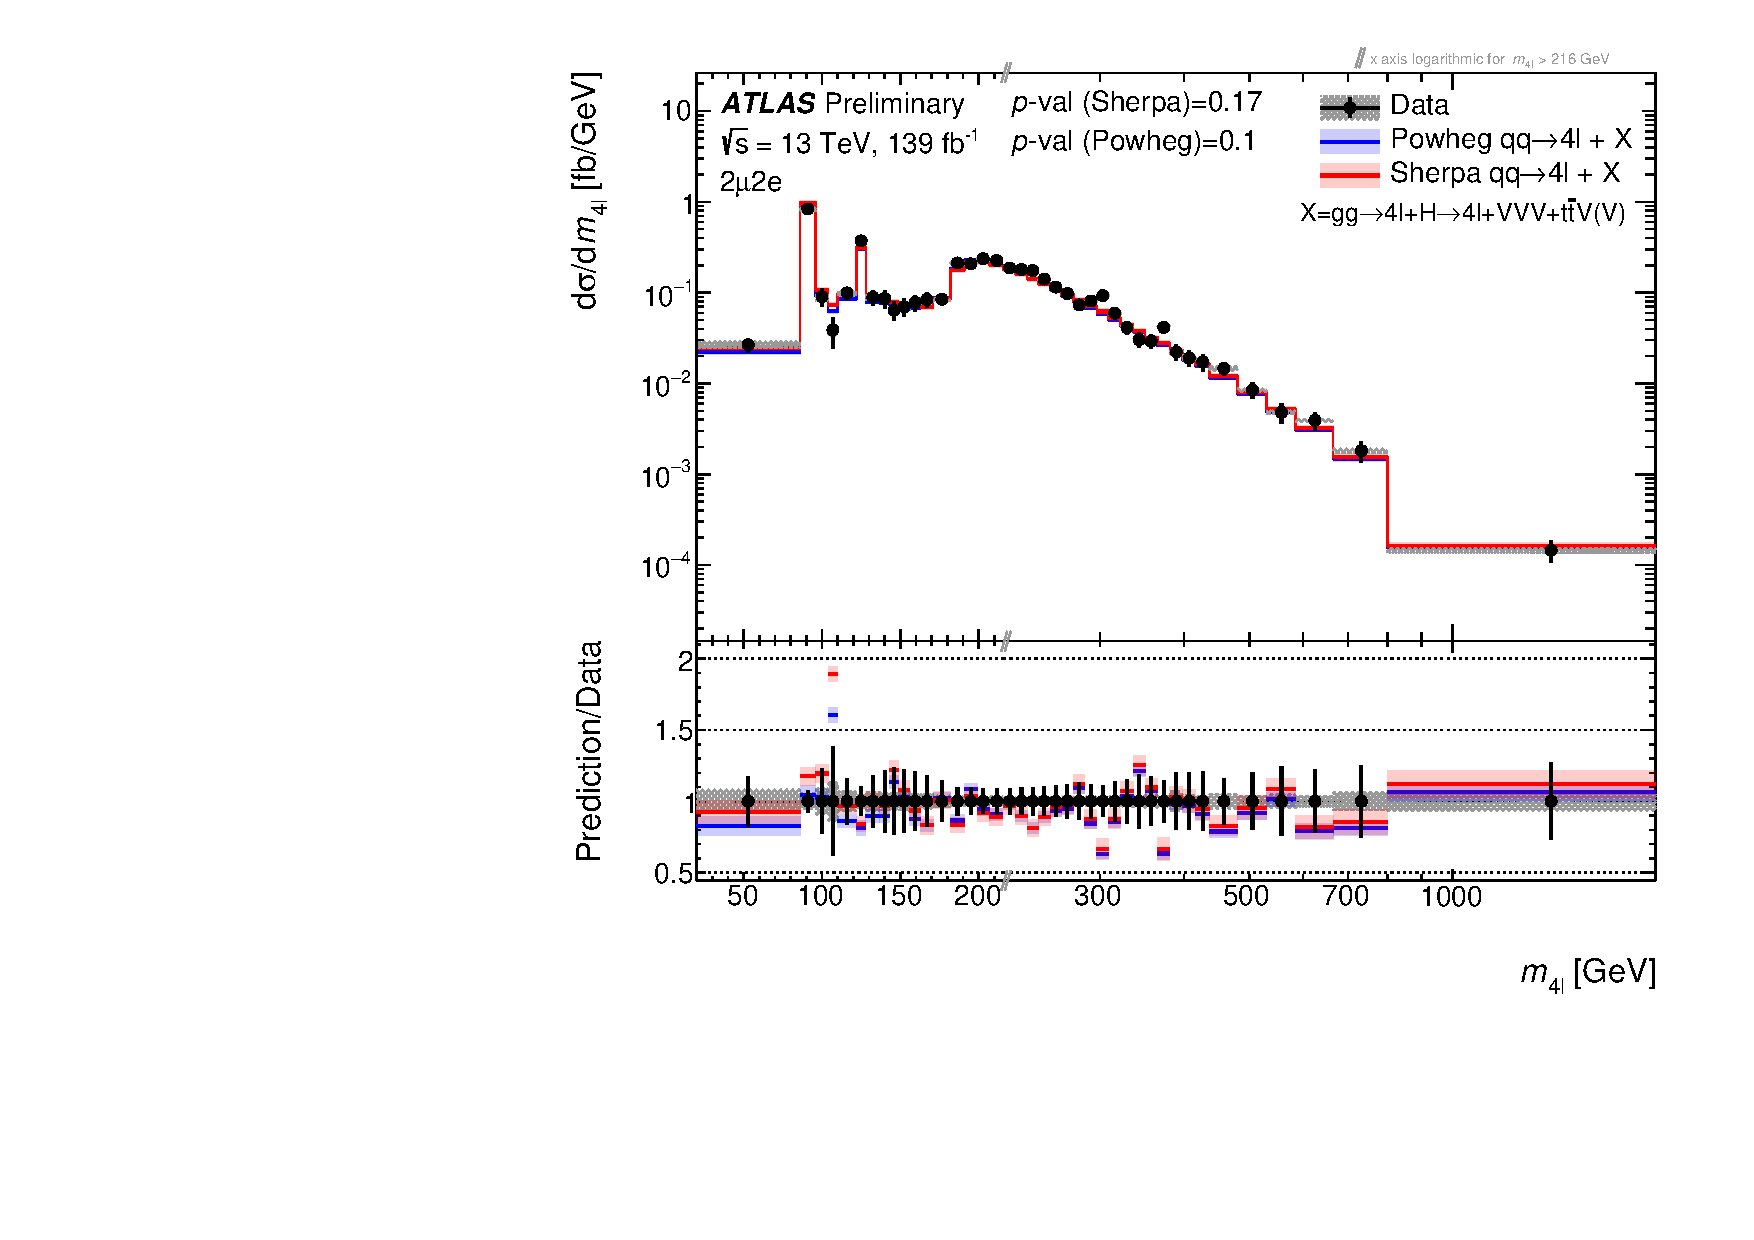
\includegraphics[width=.99\linewidth]{Figures/m4l/UnfoldedResults/linlog_Unfolded_Data_m4l_event_type2mu2e.pdf}  \caption{$2e2\mu$ channel}\label{fig:sub-third}
    \end{subfigure}
    \caption{Differential cross-section as a function of \mFourL{} for each lepton flavour channel. The measured data (black points)  are compared with the SM prediction using either \SHERPA{} (red, with red hashed band for the uncertainty) or \POWHEG{} + \pythia{} (blue, with blue hashed band for the uncertainty) to model the \qqFourL{} contribution. The error bars on the data points give the total uncertainty and the grey hashed band gives the systematic uncertainty. \Pvalue{} The lower panel shows the ratio of the SM predictions to the data.  The $x$-axis is on a linear scale until $\mFourL = 225$~\GeV, where it switches to a logarithmic scale.}
    \label{fig:m4l_flavour}
\end{figure}

%% m12 vs m4l
\begin{figure}[htb!]
    \begin{subfigure}{.49\textwidth}\centering
      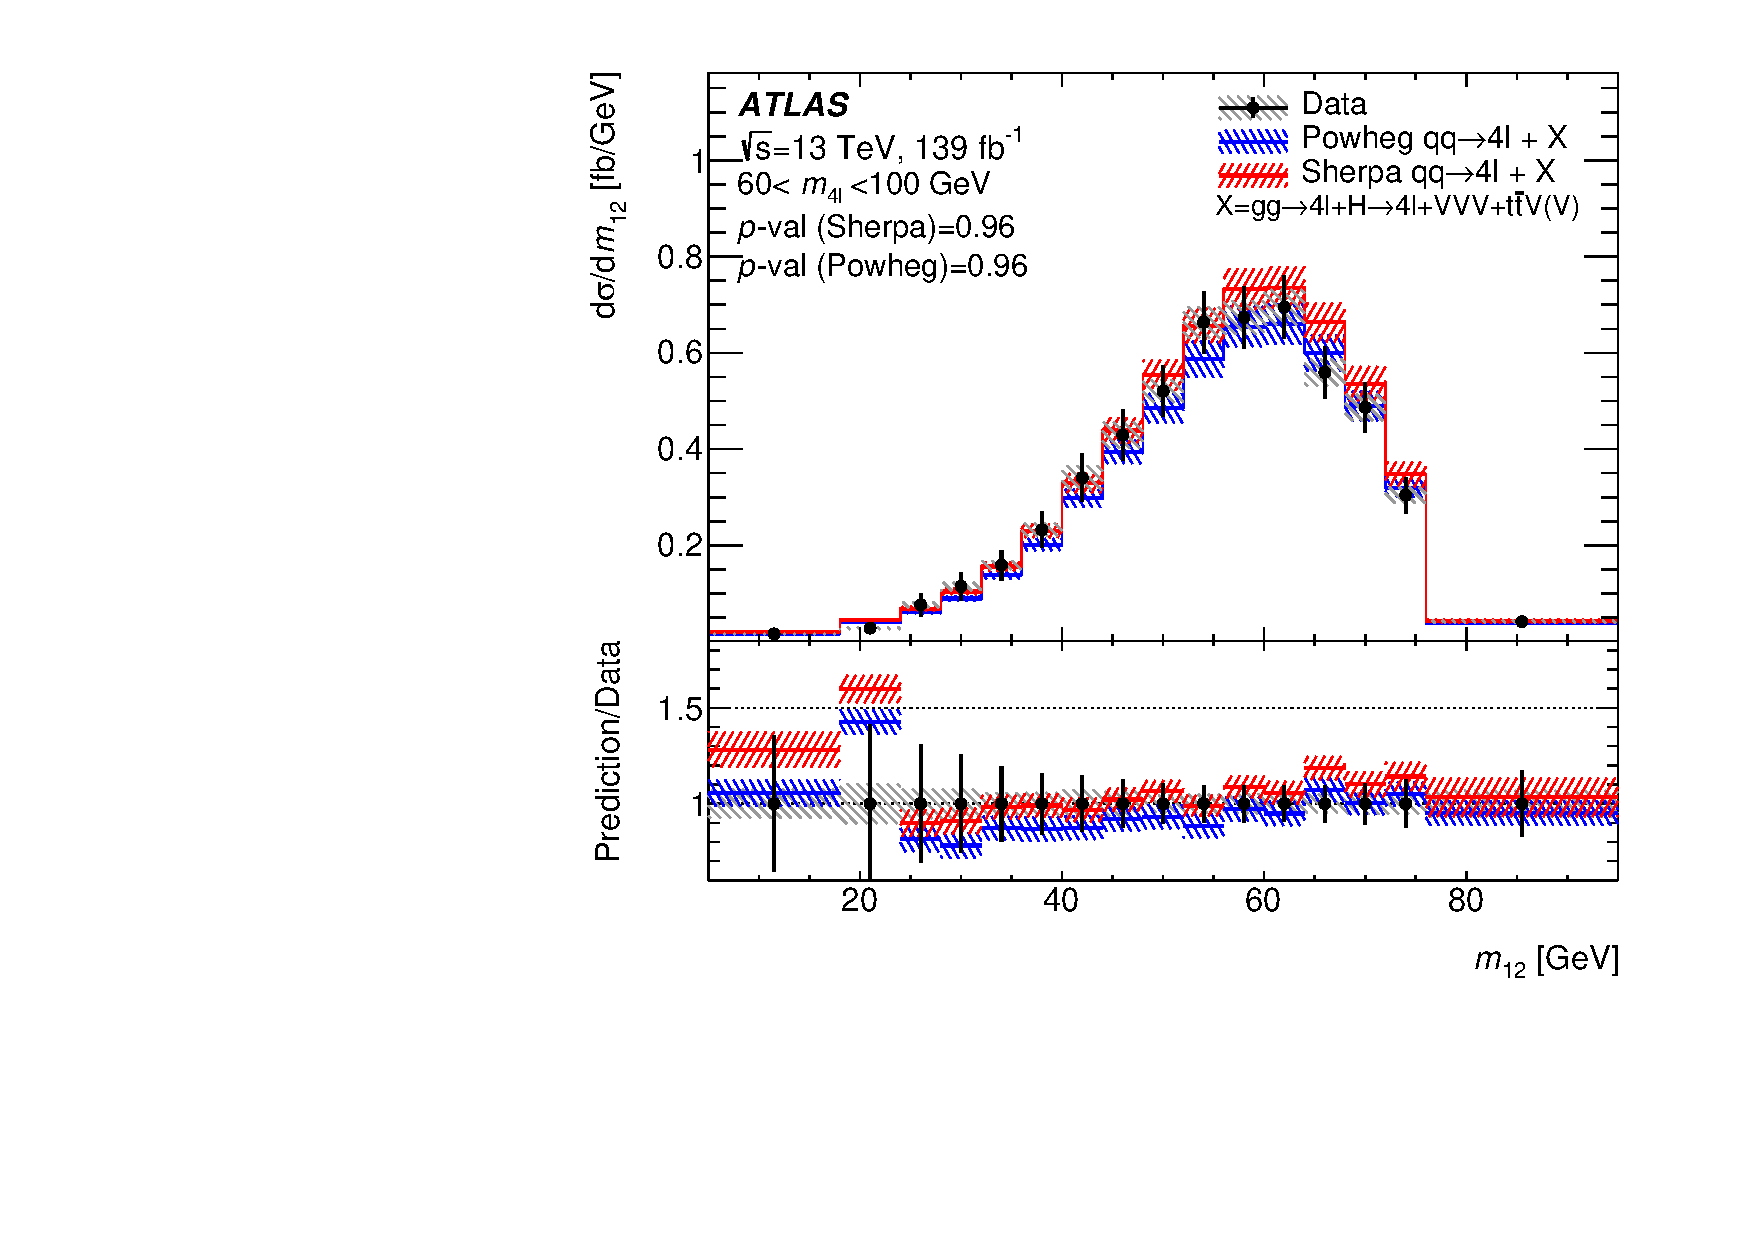
\includegraphics[width=.99\linewidth]{Figures/m4l/UnfoldedResults/linY_Unfolded_Data_m12_m4l60-100.pdf}  
      \caption{\ZFourL \ region}
      \label{fig:sub-first}
    \end{subfigure}
    \begin{subfigure}{.49\textwidth}\centering
      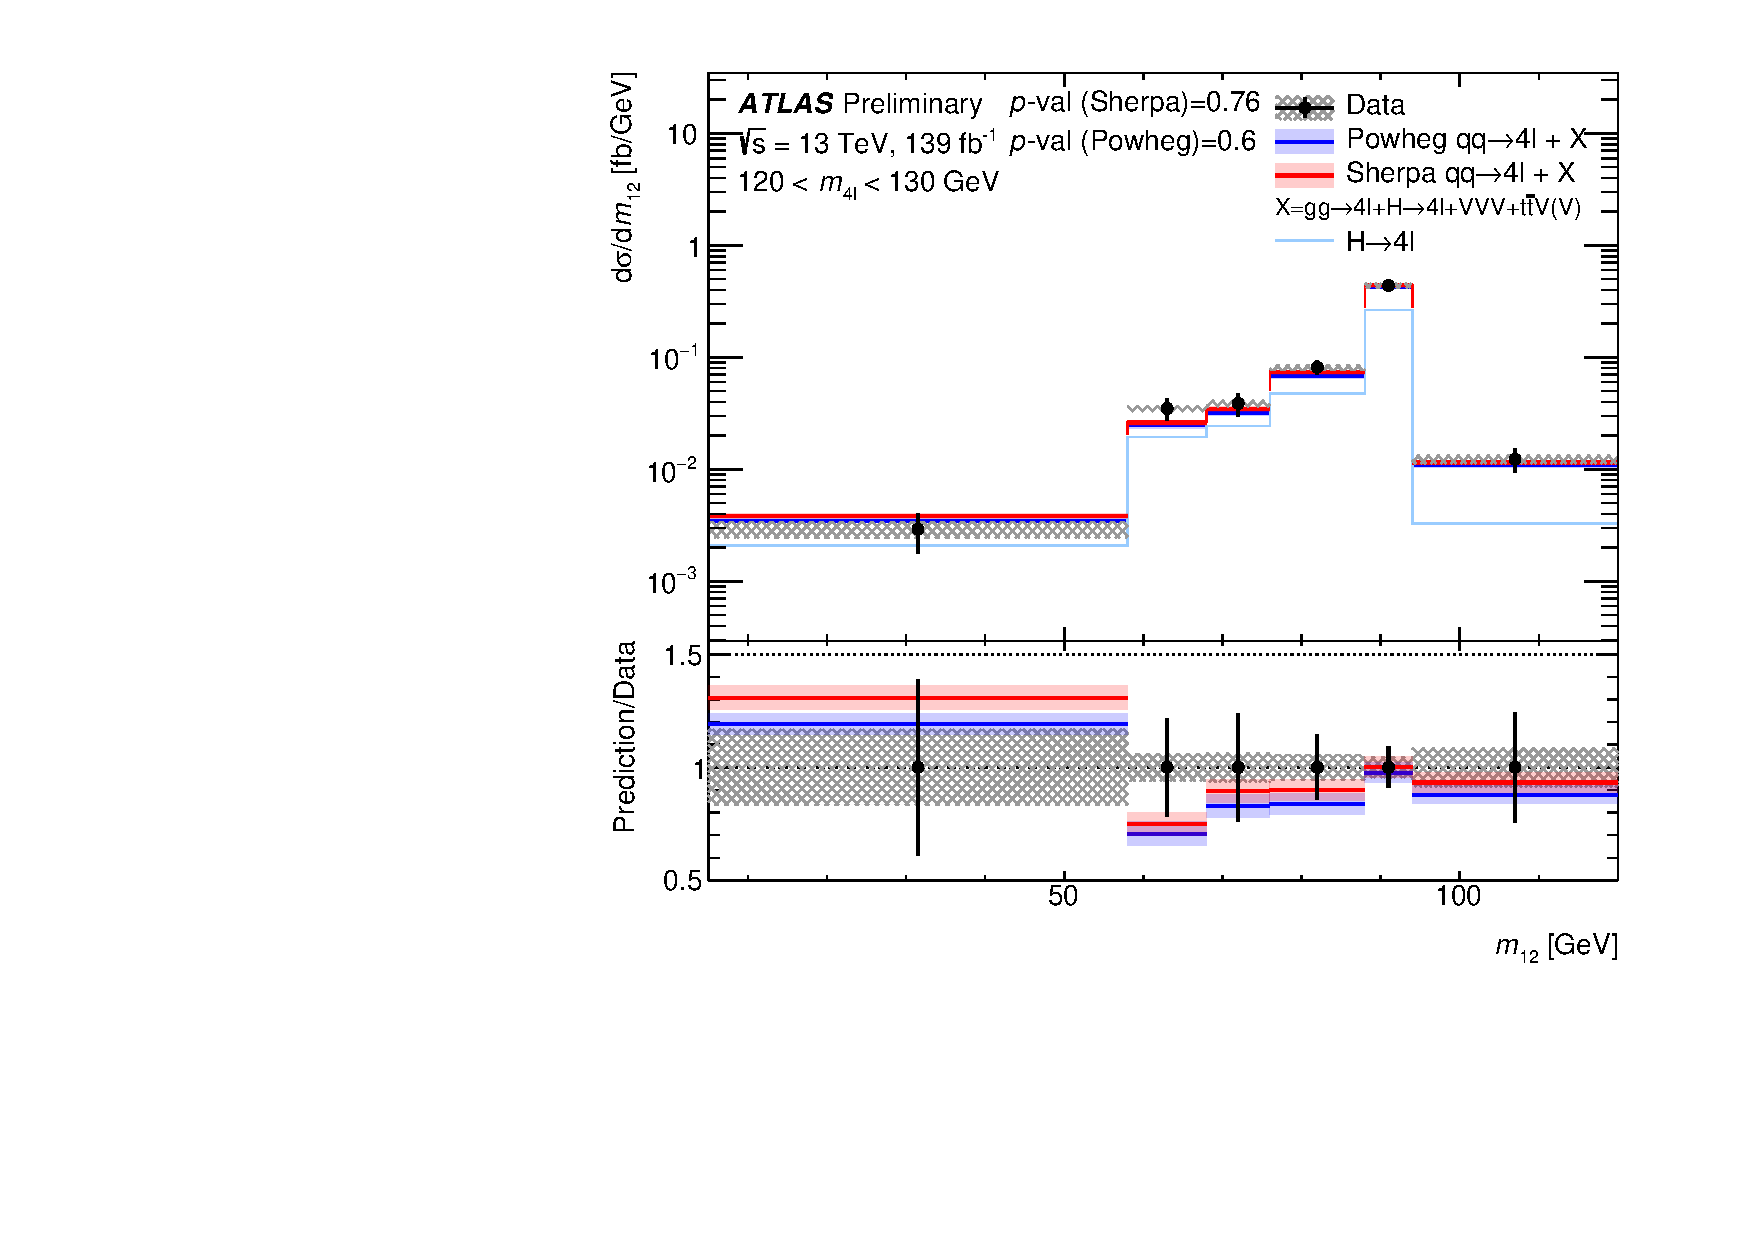
\includegraphics[width=.99\linewidth]{Figures/m4l/UnfoldedResults/higgs_Unfolded_Data_m12_m4l120-130.pdf}  
      \caption{\HFourL \ region}
      \label{fig:sub-second}
    \end{subfigure}
    \begin{subfigure}{.49\textwidth}
      \centering
      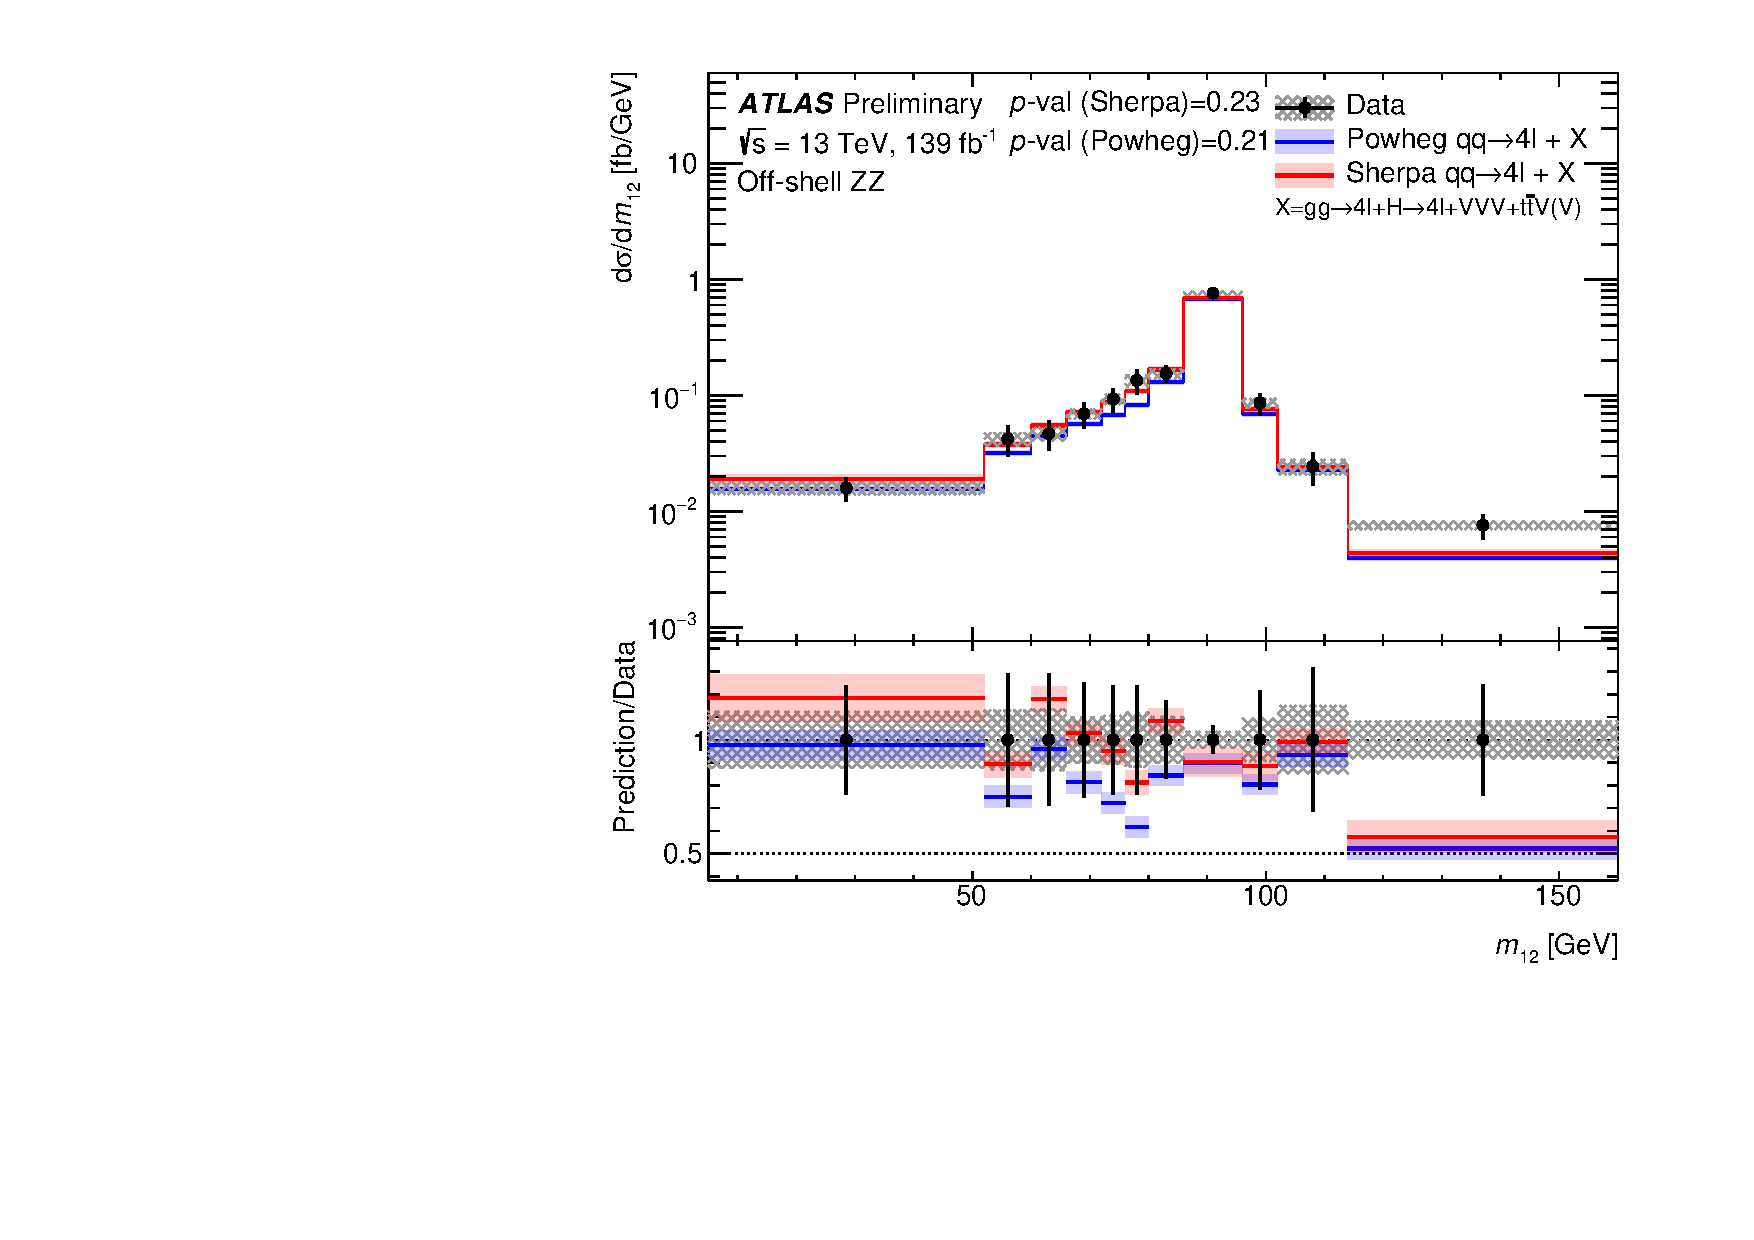
\includegraphics[width=.99\linewidth]{Figures/m4l/UnfoldedResults/Unfolded_Data_m12_m4loffshell.pdf}  
      \caption{Off-shell $\Z\Z$ region}
      \label{fig:sub-third}
    \end{subfigure}
    \begin{subfigure}{.49\textwidth}
      \centering
      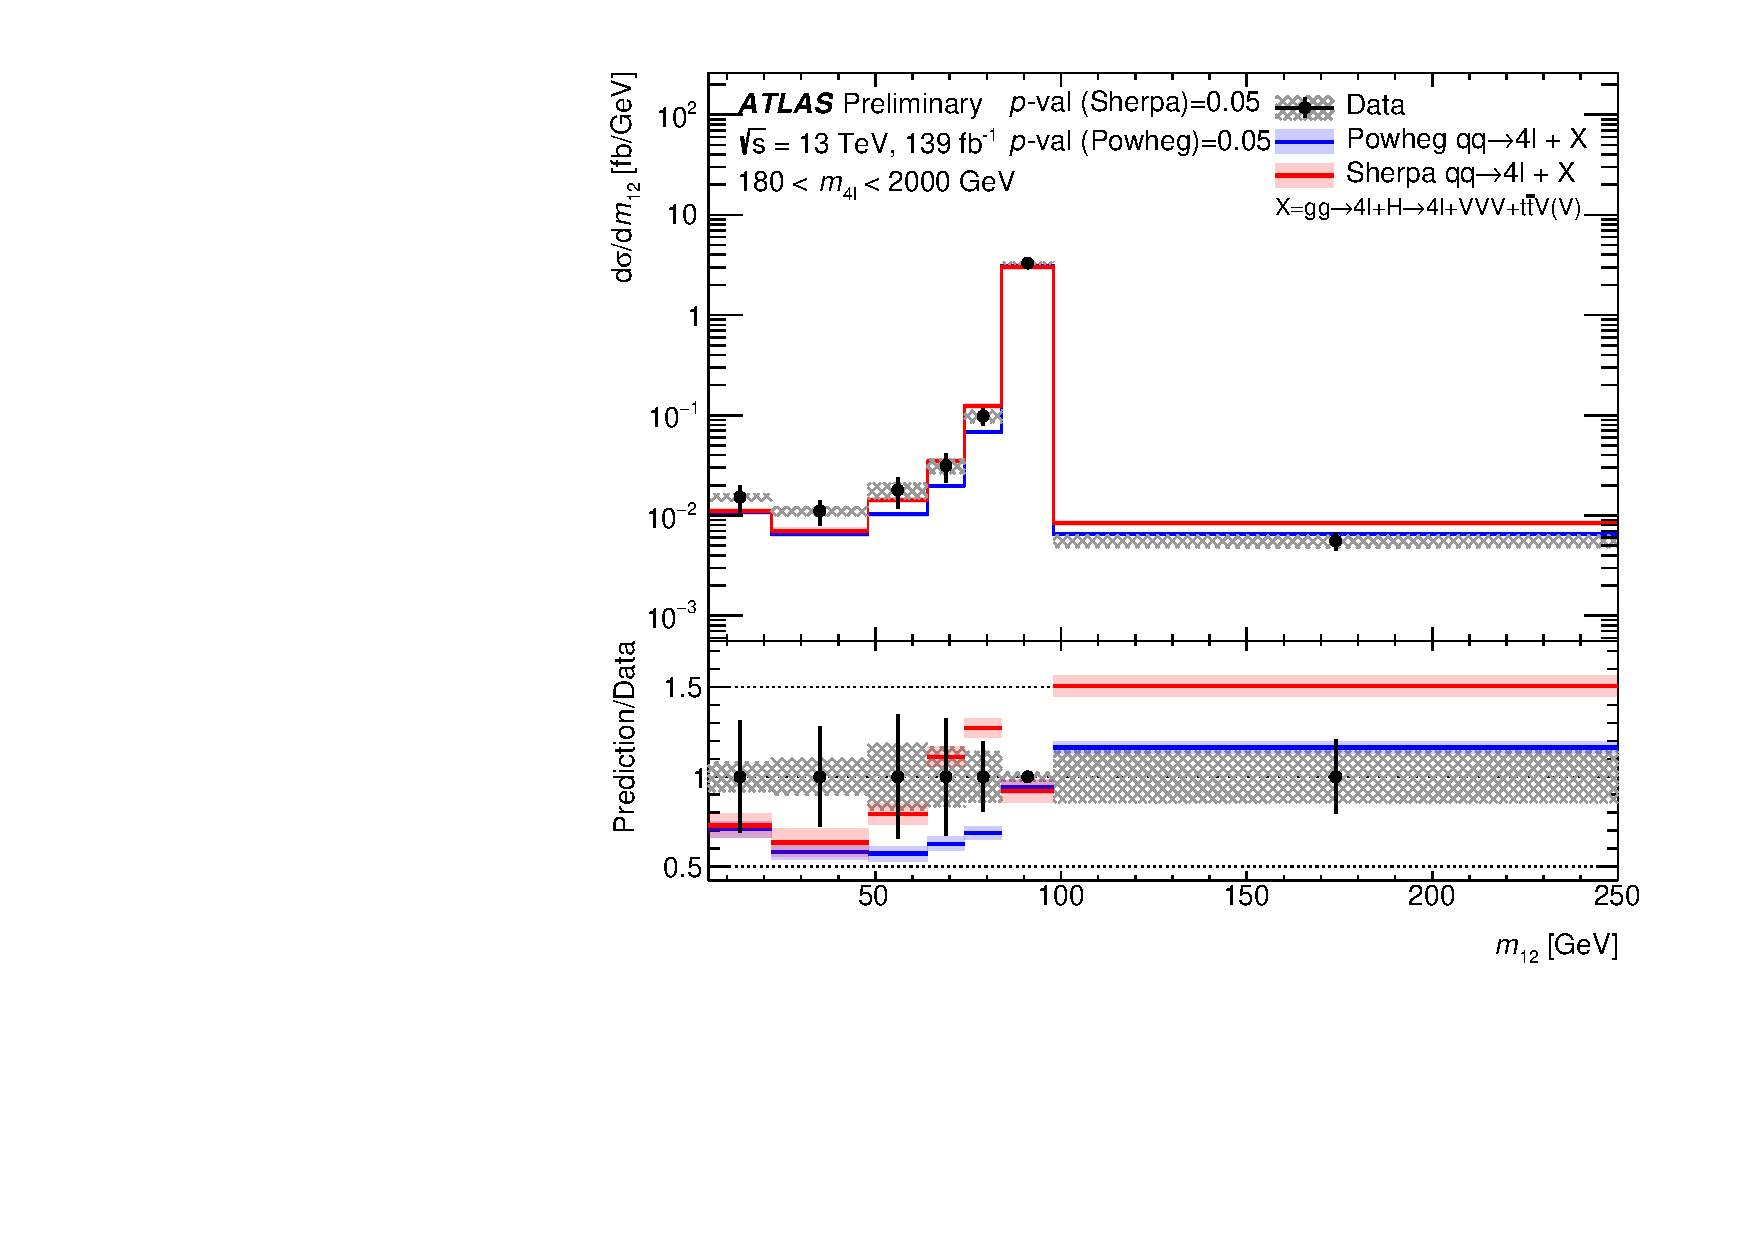
\includegraphics[width=.99\linewidth]{Figures/m4l/UnfoldedResults/Unfolded_Data_m12_m4l180-2000.pdf}  
      \caption{On-shell $\Z\Z$ region}
      \label{fig:sub-fourth}
    \end{subfigure}
    \caption{Differential cross-section as a function of \mZOne{} in the four
        \mFourL{} regions. The measured data (black points) are  compared with the SM prediction using either \SHERPA{} (red, with red hashed band for the uncertainty) or \POWHEG{} + \pythia{} (blue, with blue hashed band for the uncertainty) to model the \qqFourL{} contribution. In (b) the contribution from Higgs production is shown in addition to the total SM prediction. The error bars on the data points give the total uncertainty and the grey hashed band gives the systematic uncertainty. \Pvalue{} The  lower panel shows the ratio of the SM predictions to the data.}
    \label{fig:m12_m4l}
\end{figure}

%% m34 vs m4l
\begin{figure}[htb!]
    \begin{subfigure}{.49\textwidth}\centering
      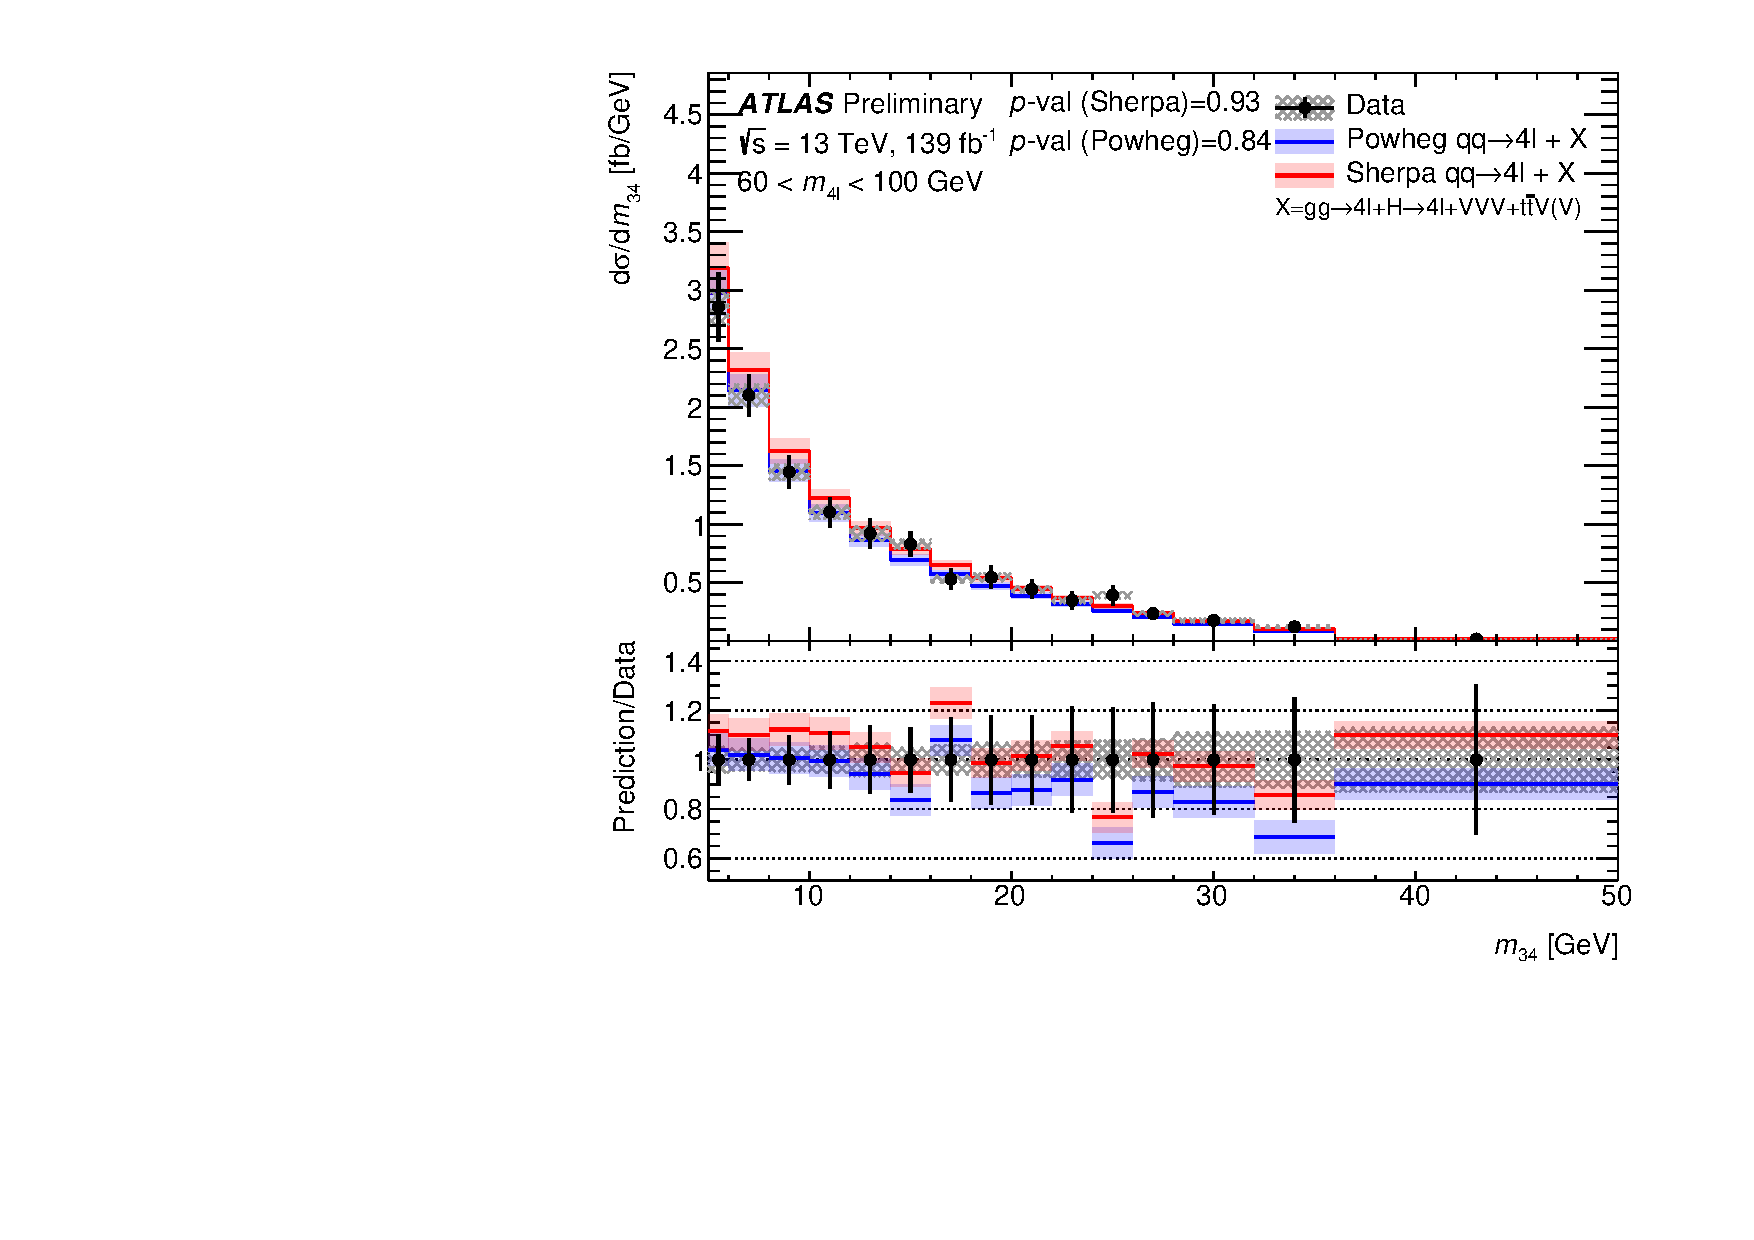
\includegraphics[width=.99\linewidth]{Figures/m4l/UnfoldedResults/linY_Unfolded_Data_m34_m4l60-100.pdf}\caption{\ZFourL \ region}\label{fig:sub-first}
    \end{subfigure}
    \begin{subfigure}{.49\textwidth}\centering
      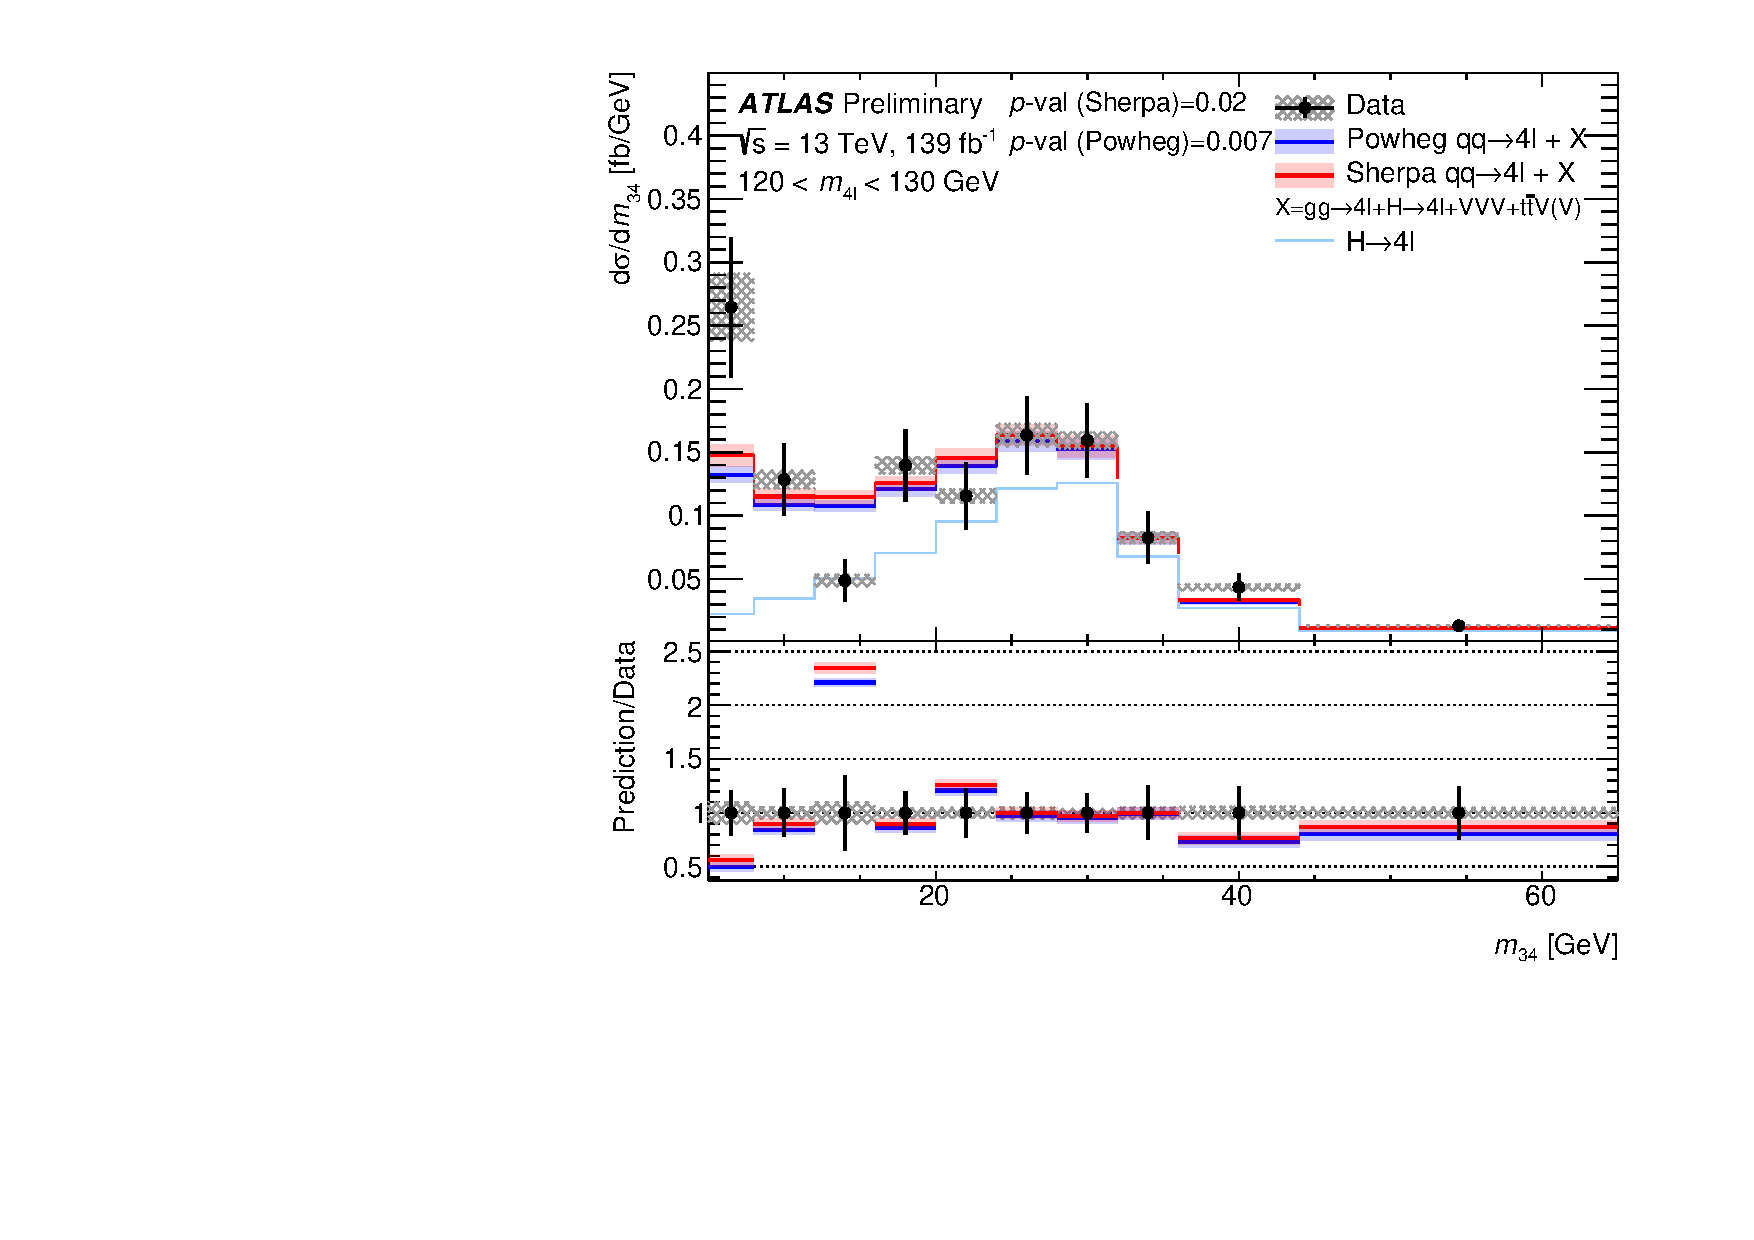
\includegraphics[width=.99\linewidth]{Figures/m4l/UnfoldedResults/higgs_linY_Unfolded_Data_m34_m4l120-130.pdf} \caption{\HFourL \ region}\label{fig:sub-second}
    \end{subfigure}
    \begin{subfigure}{.49\textwidth}\centering
      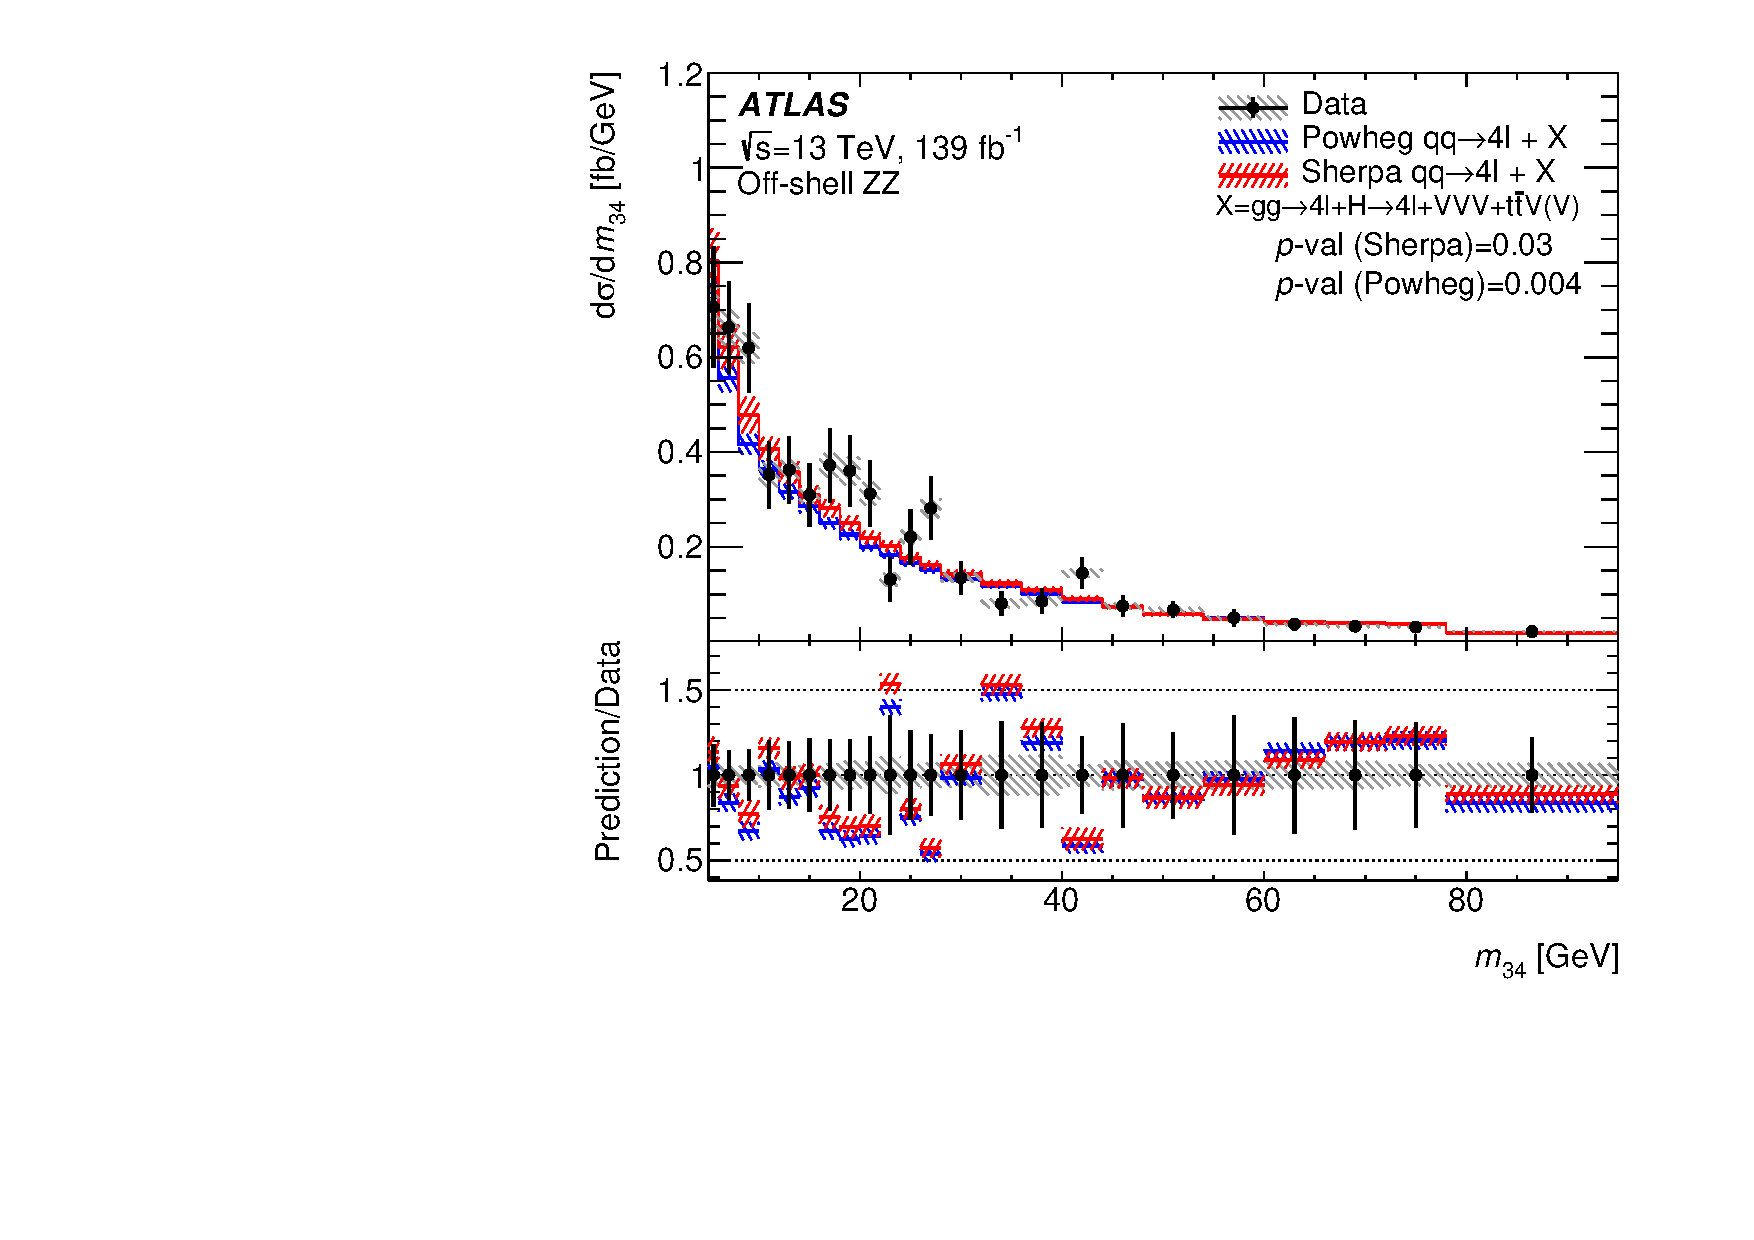
\includegraphics[width=.99\linewidth]{Figures/m4l/UnfoldedResults/linY_Unfolded_Data_m34_m4loffshell.pdf}  \caption{Off-shell $\Z\Z$ region}\label{fig:sub-third}
    \end{subfigure}
    \begin{subfigure}{.49\textwidth}\centering
      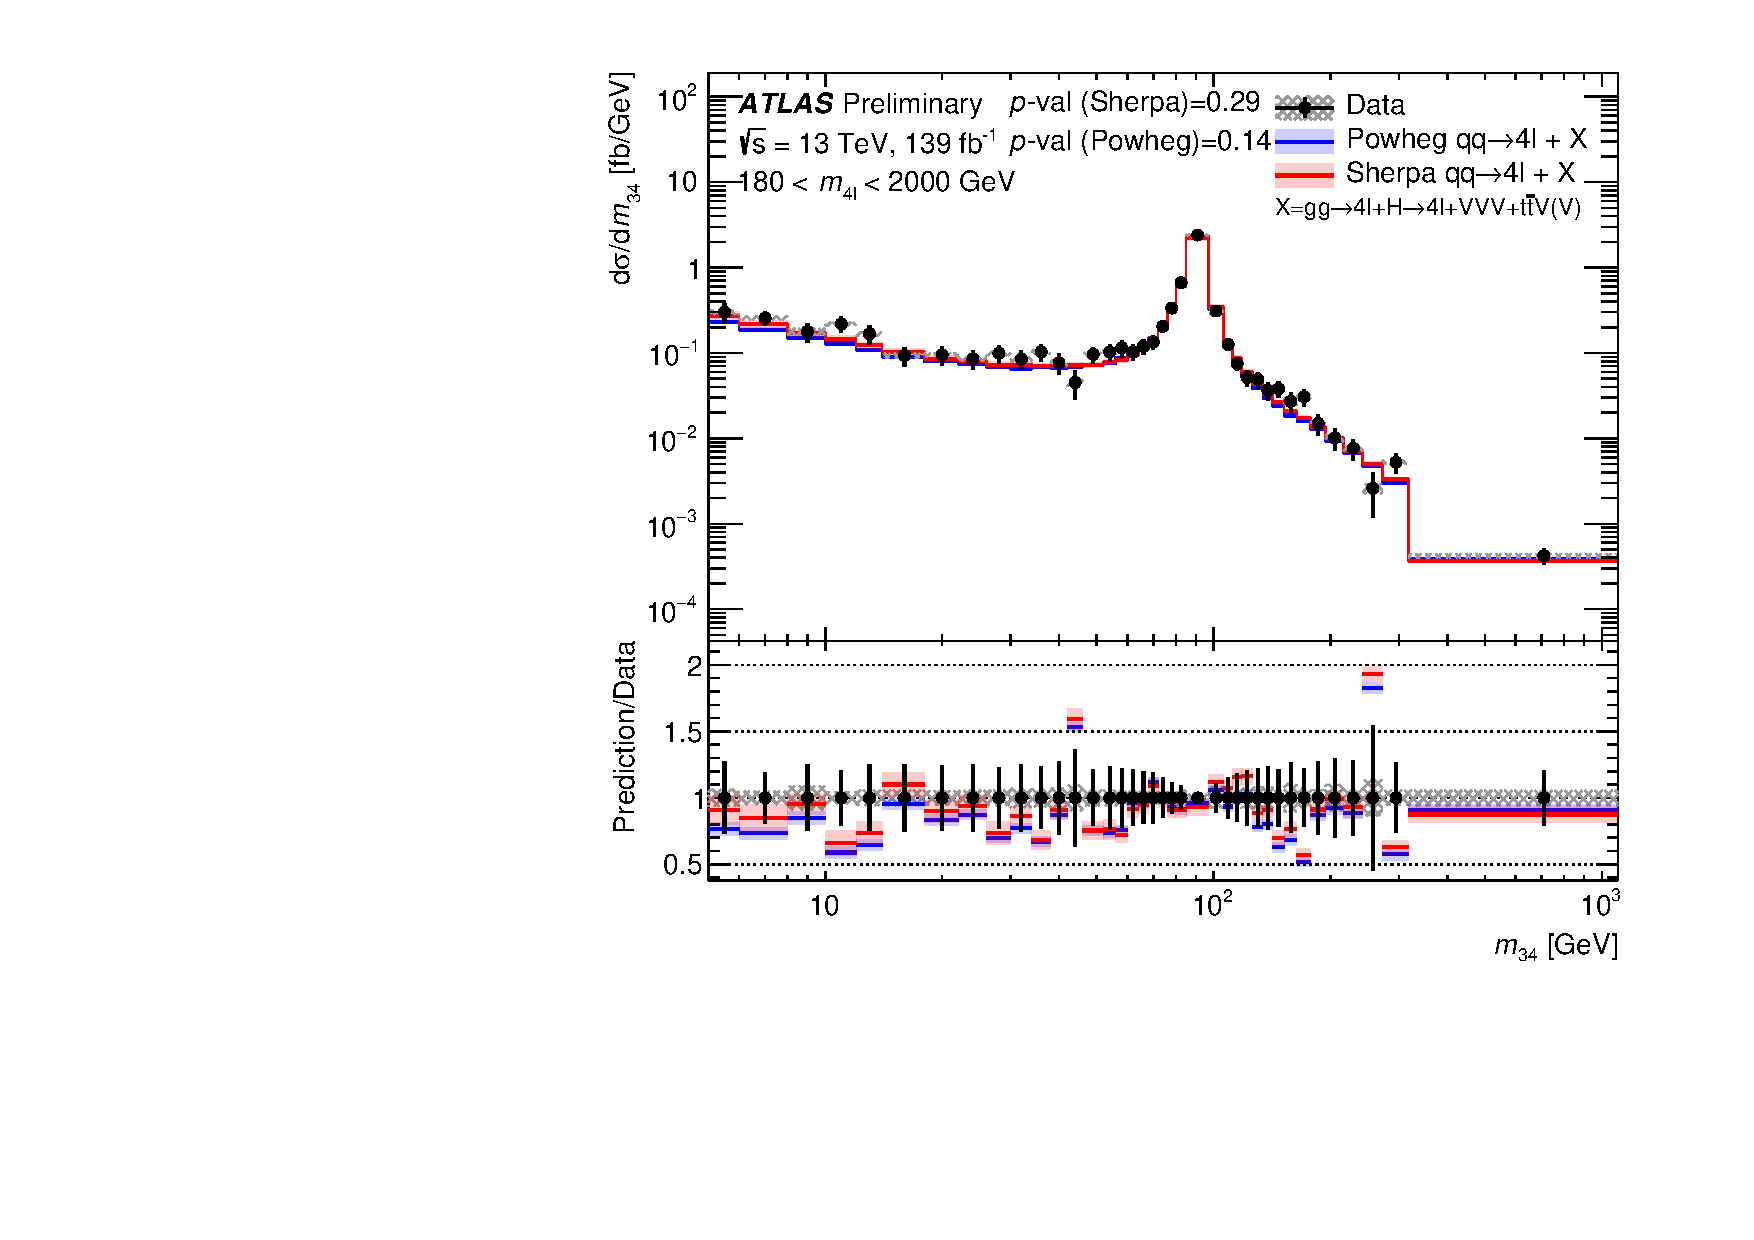
\includegraphics[width=.99\linewidth]{Figures/m4l/UnfoldedResults/Unfolded_Data_m34_m4l180-2000.pdf}  \caption{On-shell $\Z\Z$ region}\label{fig:sub-fourth}
    \end{subfigure}
    \caption{Differential cross-section as a function of \mZTwo{} in the four
        \mFourL{} regions. The measured data (black points) are  compared with the SM prediction using either \SHERPA{} (red, with red hashed band for the uncertainty) or \POWHEG{} + \pythia{} (blue, with blue hashed band for the uncertainty) to model the \qqFourL{} contribution. In (b) the contribution from Higgs production is shown in addition to the total SM prediction. The error bars on the data points give the total uncertainty and the grey hashed band gives the systematic uncertainty. \Pvalue{} The  lower panel shows the ratio of the SM predictions to the data.}
    \label{fig:m34_m4l}
\end{figure}

%% pt12 vs m4l
\begin{figure}[htb!]
    \begin{subfigure}{.49\textwidth}\centering
      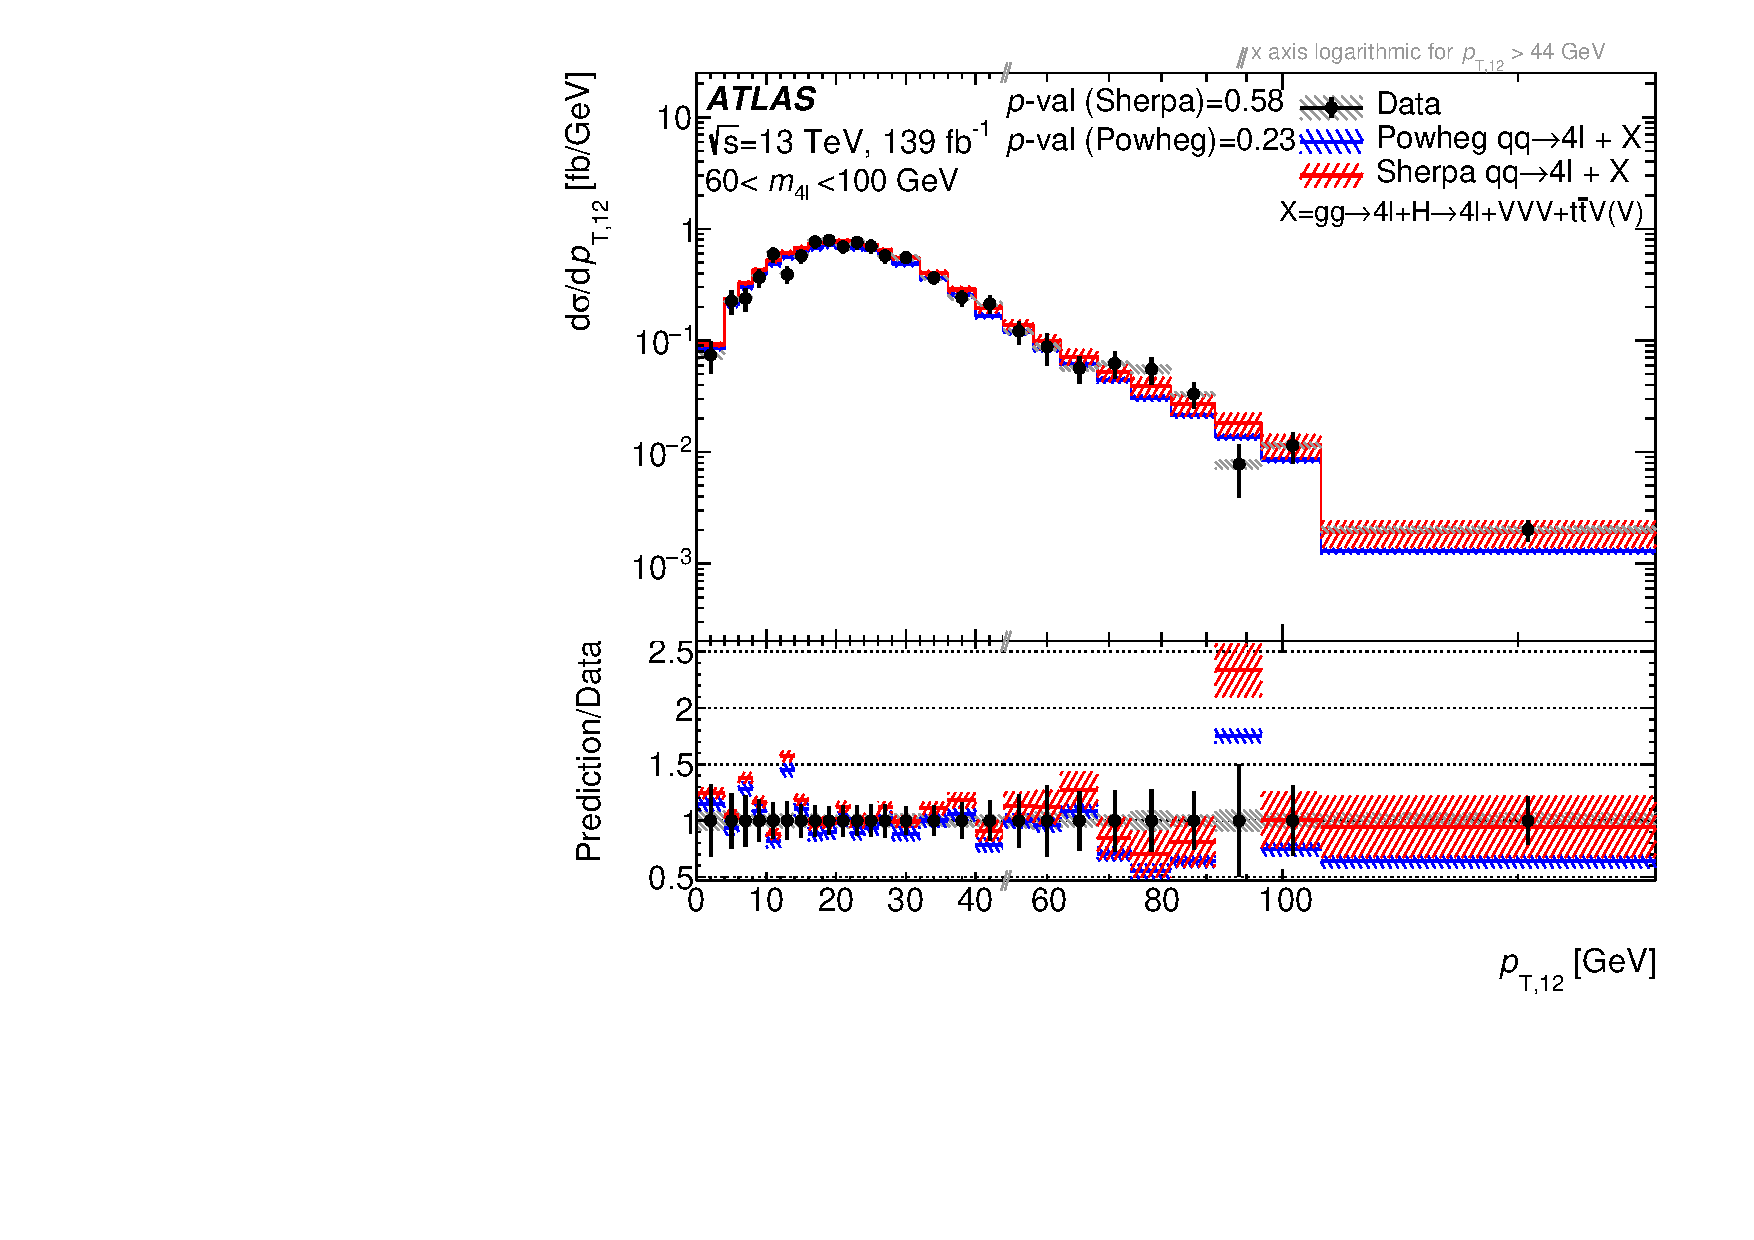
\includegraphics[width=.99\linewidth]{Figures/m4l/UnfoldedResults/linlog_Unfolded_Data_pt12_m4l60-100.pdf}\caption{\ZFourL \ region}\label{fig:sub-first}
    \end{subfigure}
    \begin{subfigure}{.49\textwidth}\centering
      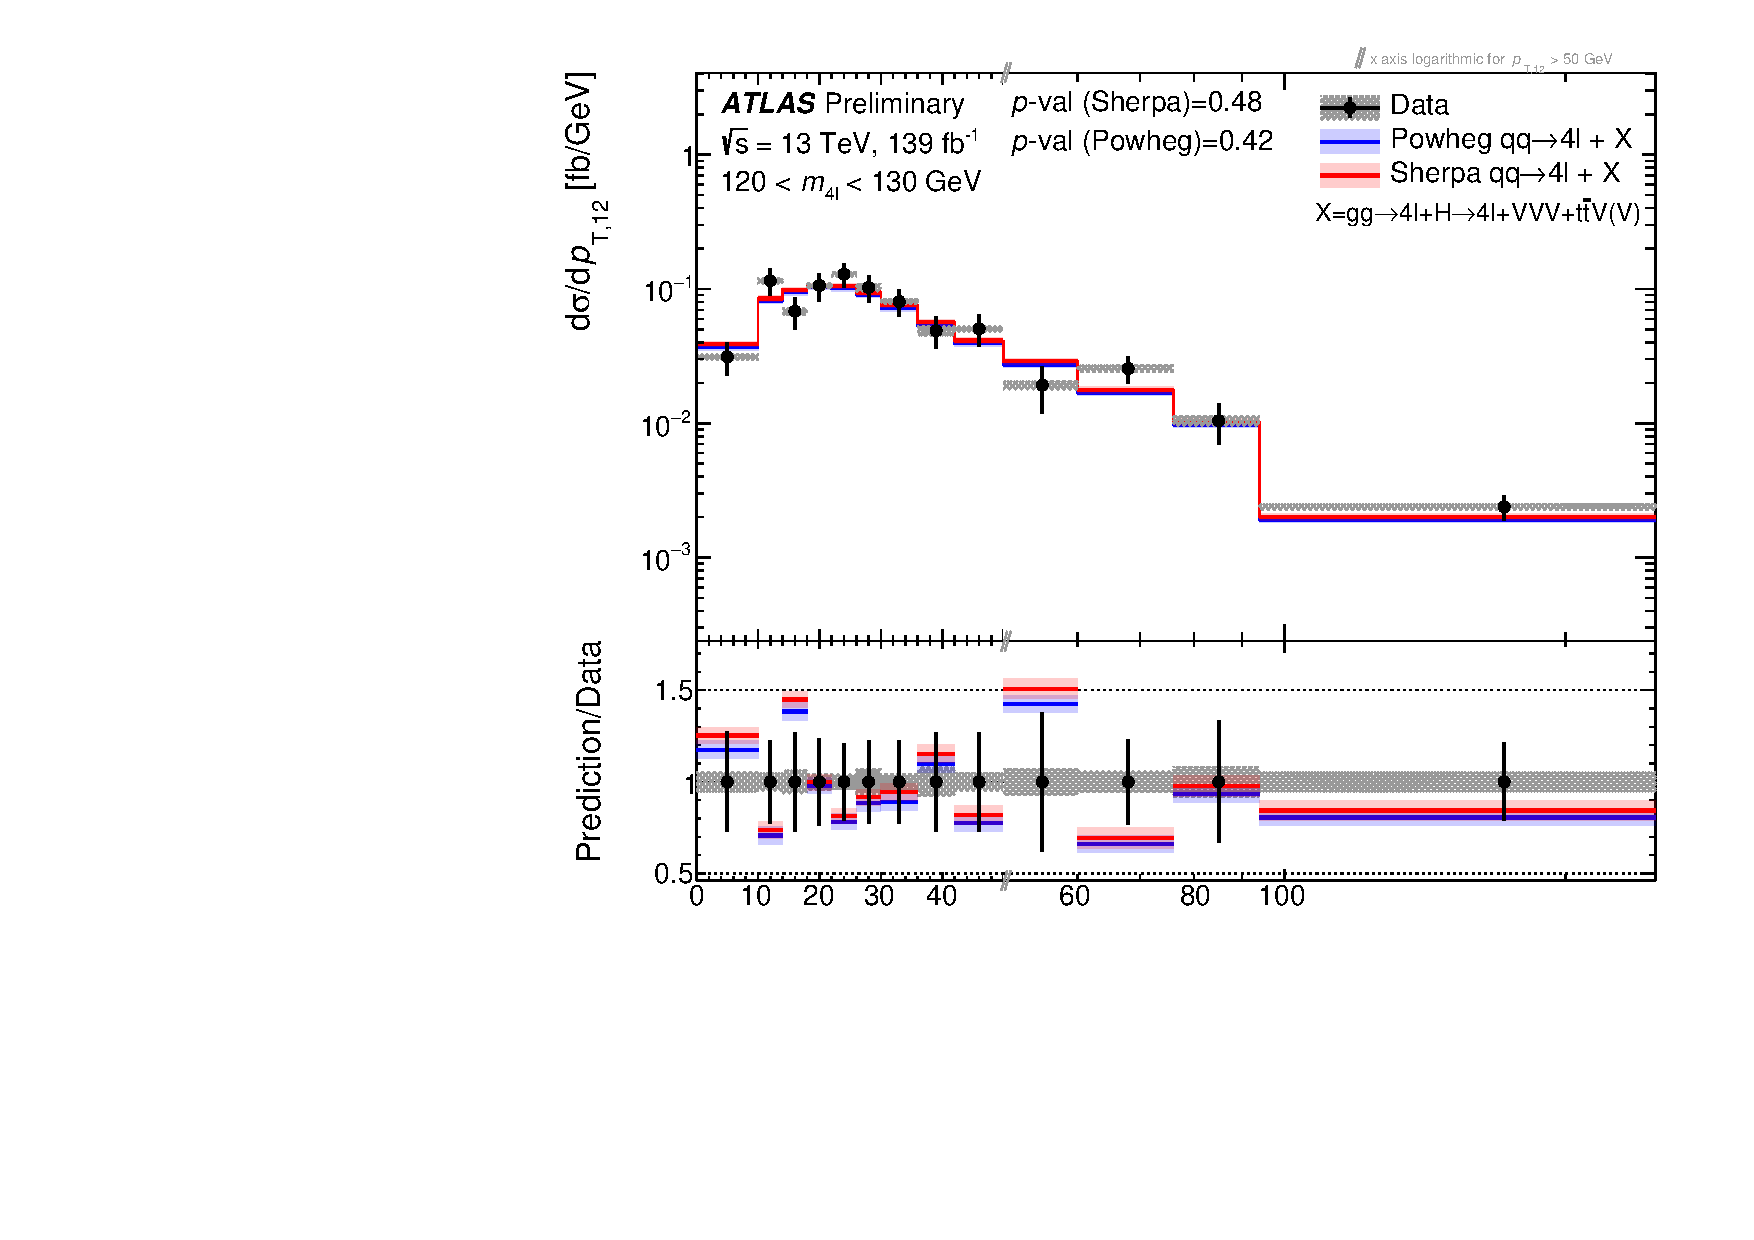
\includegraphics[width=.99\linewidth]{Figures/m4l/UnfoldedResults/linlog_Unfolded_Data_pt12_m4l120-130.pdf} \caption{\HFourL \ region}\label{fig:sub-second}
    \end{subfigure}
    \begin{subfigure}{.49\textwidth}\centering
      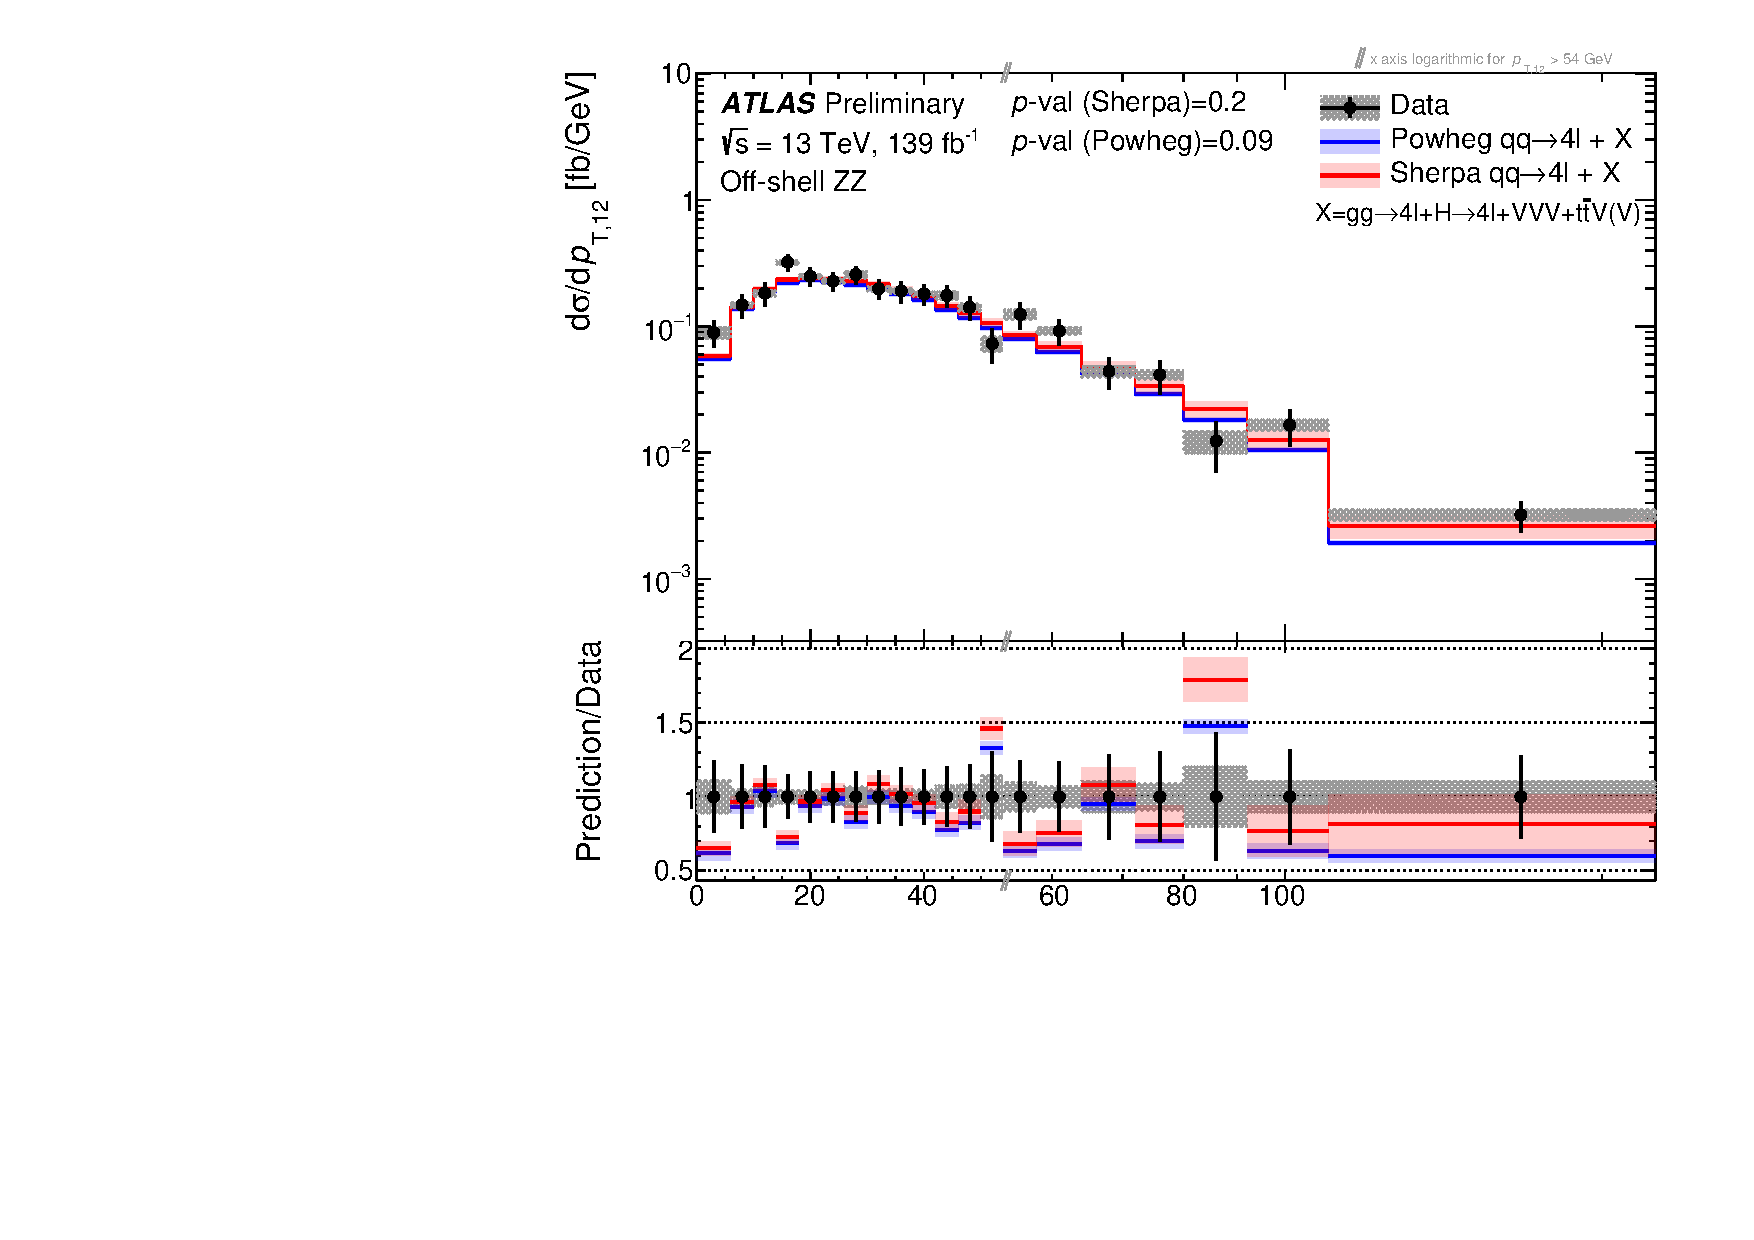
\includegraphics[width=.99\linewidth]{Figures/m4l/UnfoldedResults/linlog_Unfolded_Data_pt12_m4loffshell.pdf}  \caption{Off-shell $\Z\Z$ region}\label{fig:sub-third}
    \end{subfigure}
    \begin{subfigure}{.49\textwidth}\centering
      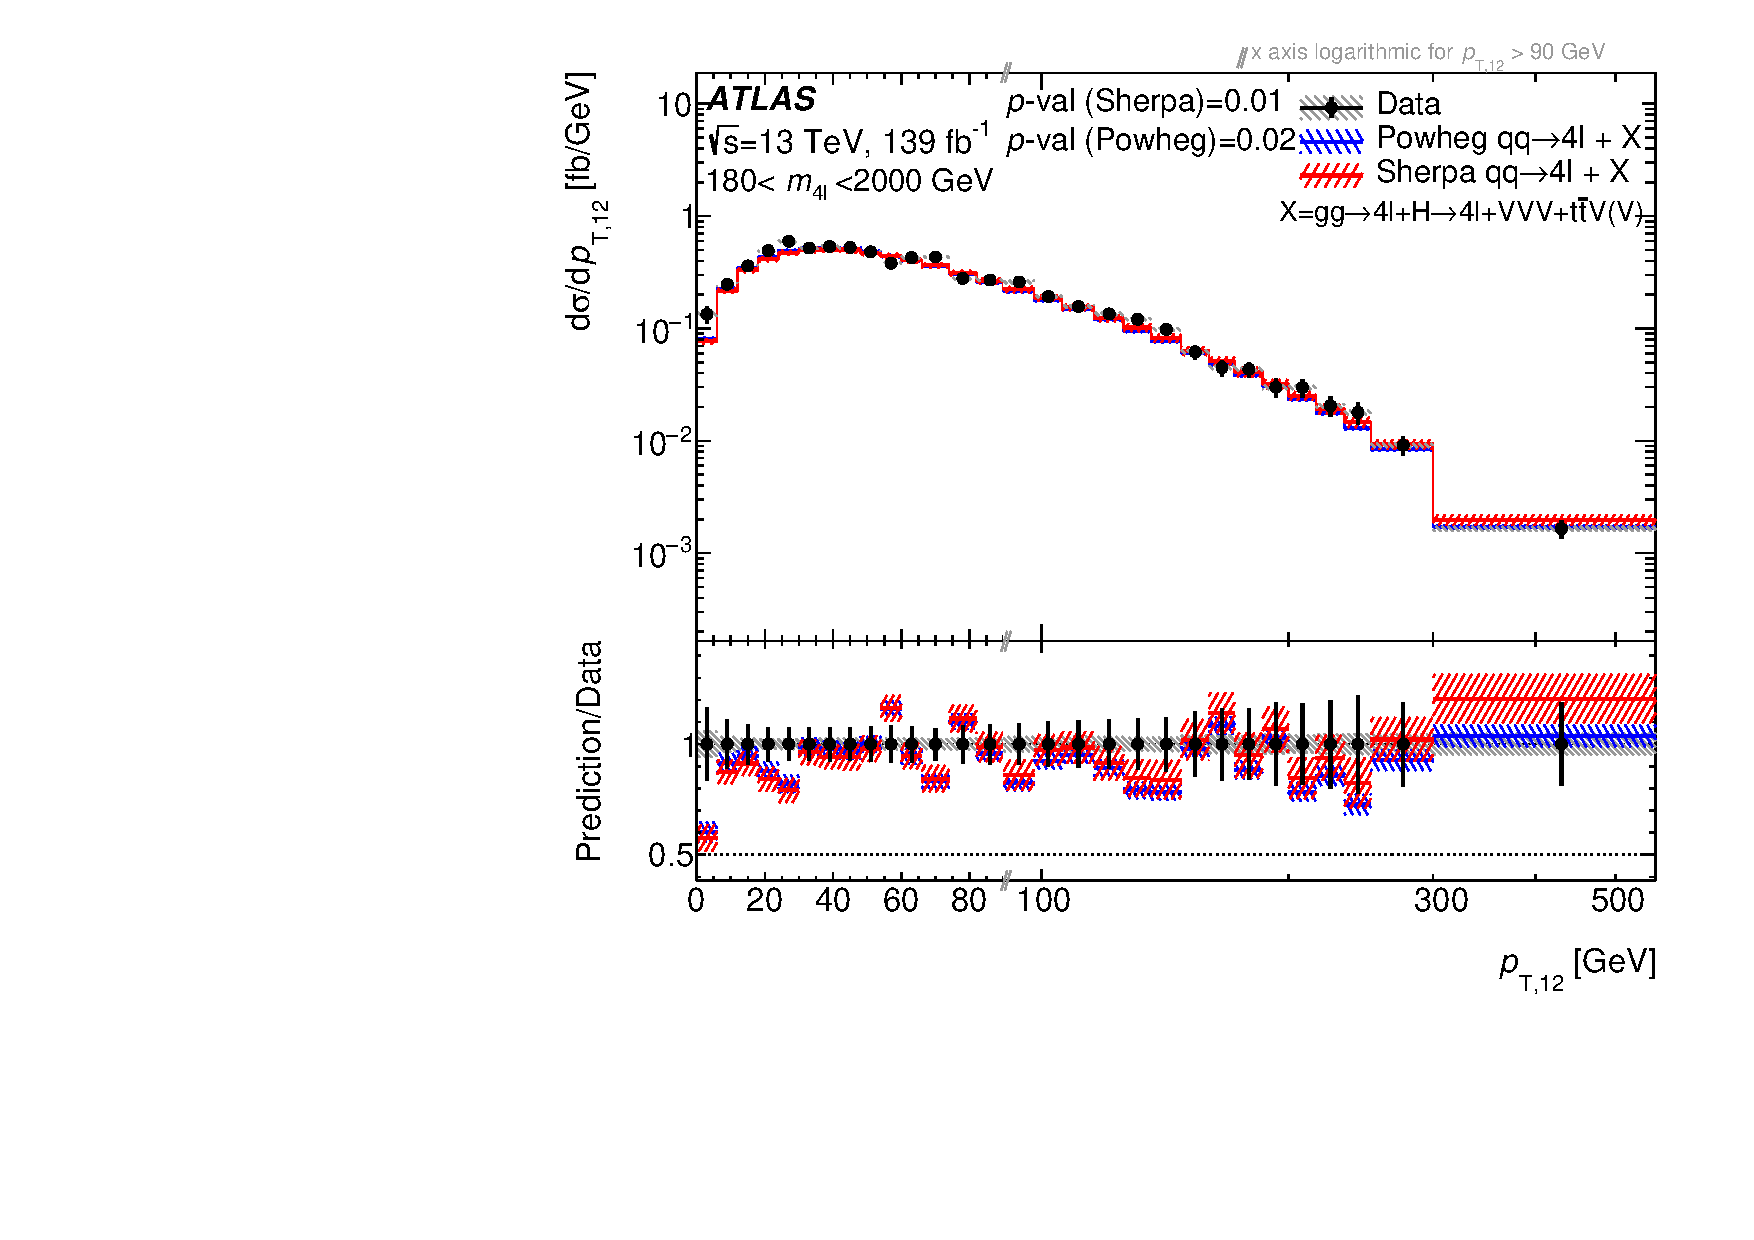
\includegraphics[width=.99\linewidth]{Figures/m4l/UnfoldedResults/linlog_Unfolded_Data_pt12_m4l180-2000.pdf}  \caption{On-shell $\Z\Z$ region}\label{fig:sub-fourth}
    \end{subfigure}
    \caption{Differential cross-section as a function of \ptZOne{} in the four
        \mFourL{} regions. The measured data (black points) are  compared with the SM prediction using either \SHERPA{} (red, with red hashed band for the uncertainty) or \POWHEG{} + \pythia{} (blue, with blue hashed band for the uncertainty) to model the \qqFourL{} contribution. In (b) the contribution from Higgs production is shown in addition to the total SM prediction. The error bars on the data points give the total uncertainty and the grey hashed band gives the systematic uncertainty. \Pvalue{} The  lower panel shows the ratio of the SM predictions to the data.}
    \label{fig:pt12_m4l}
\end{figure}

%% pt34 vs m4l
\begin{figure}[htb!]
    \begin{subfigure}{.49\textwidth}\centering
      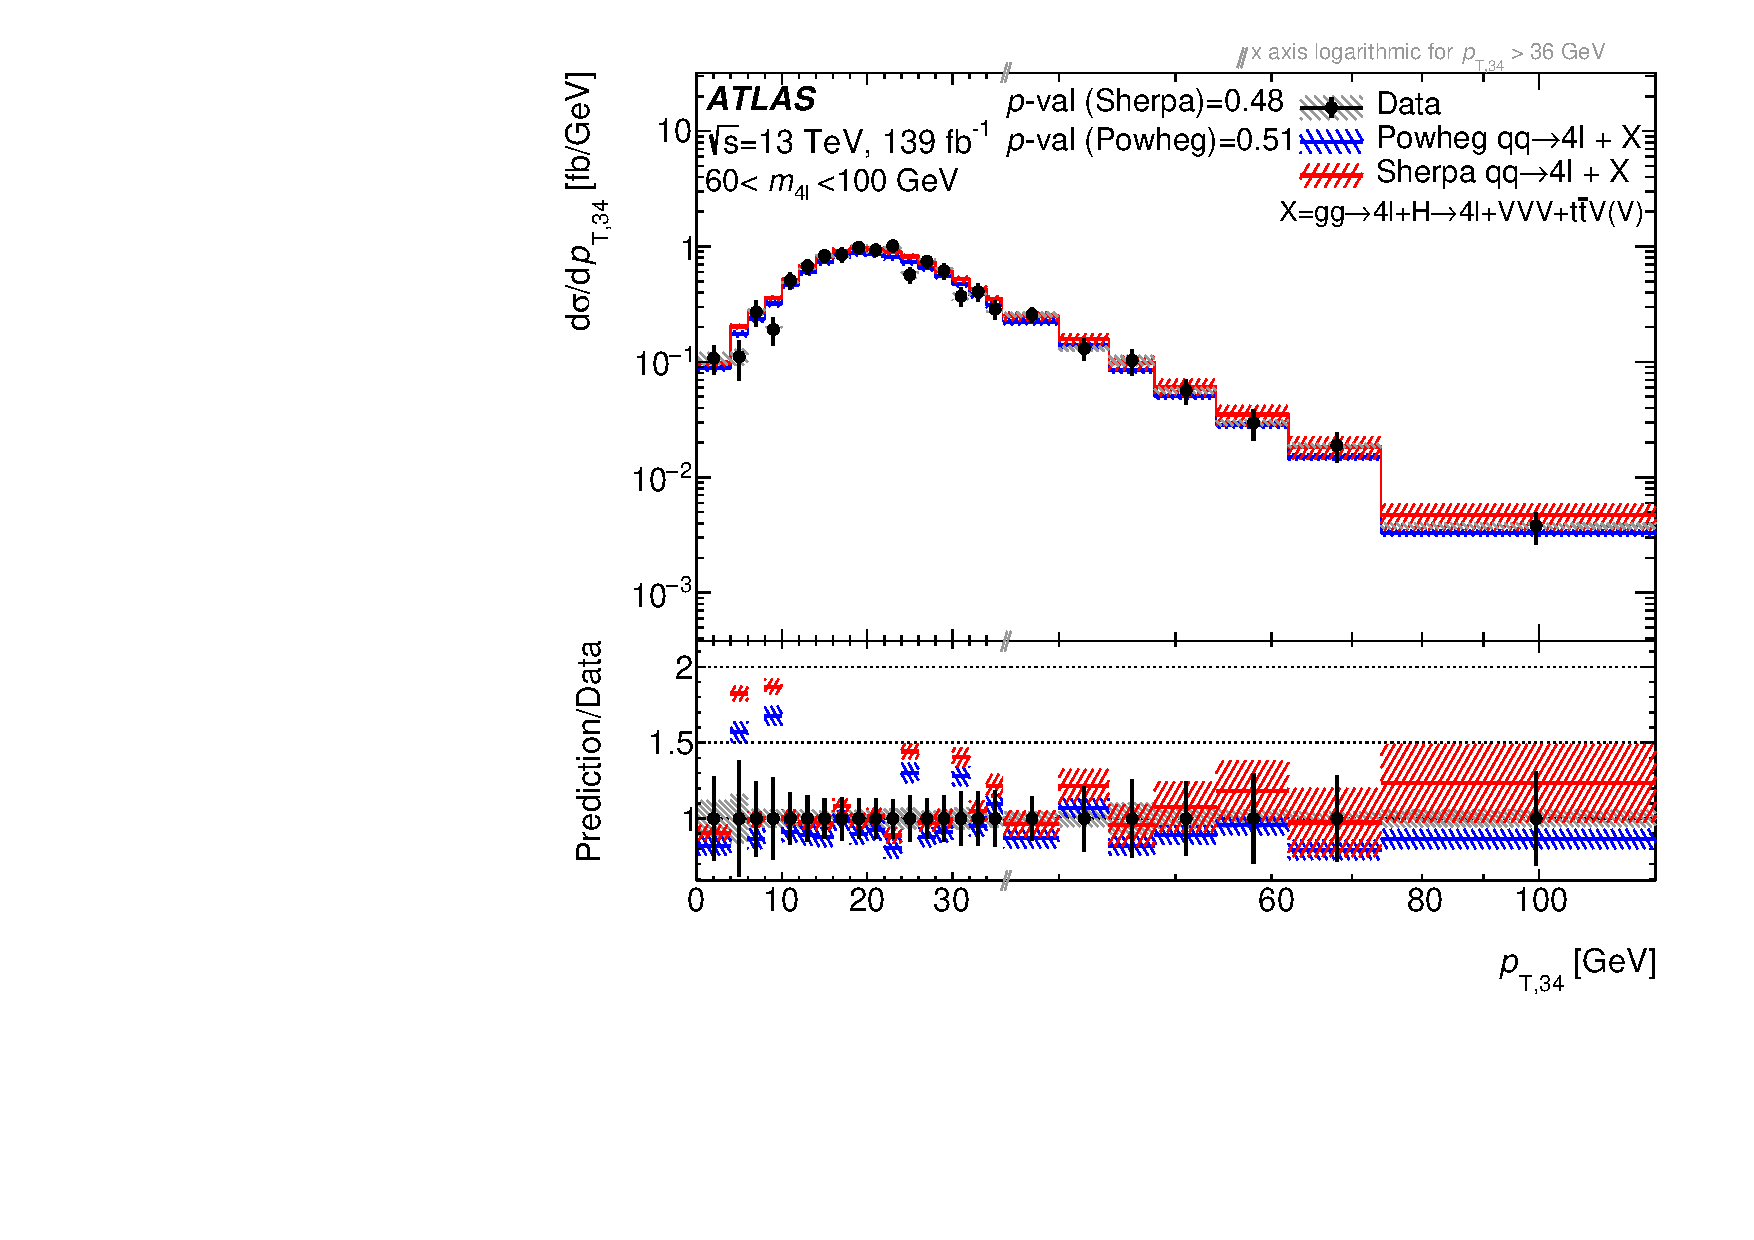
\includegraphics[width=.99\linewidth]{Figures/m4l/UnfoldedResults/linlog_Unfolded_Data_pt34_m4l60-100.pdf}\caption{\ZFourL \ region}\label{fig:sub-first}
    \end{subfigure}
    \begin{subfigure}{.49\textwidth}\centering
      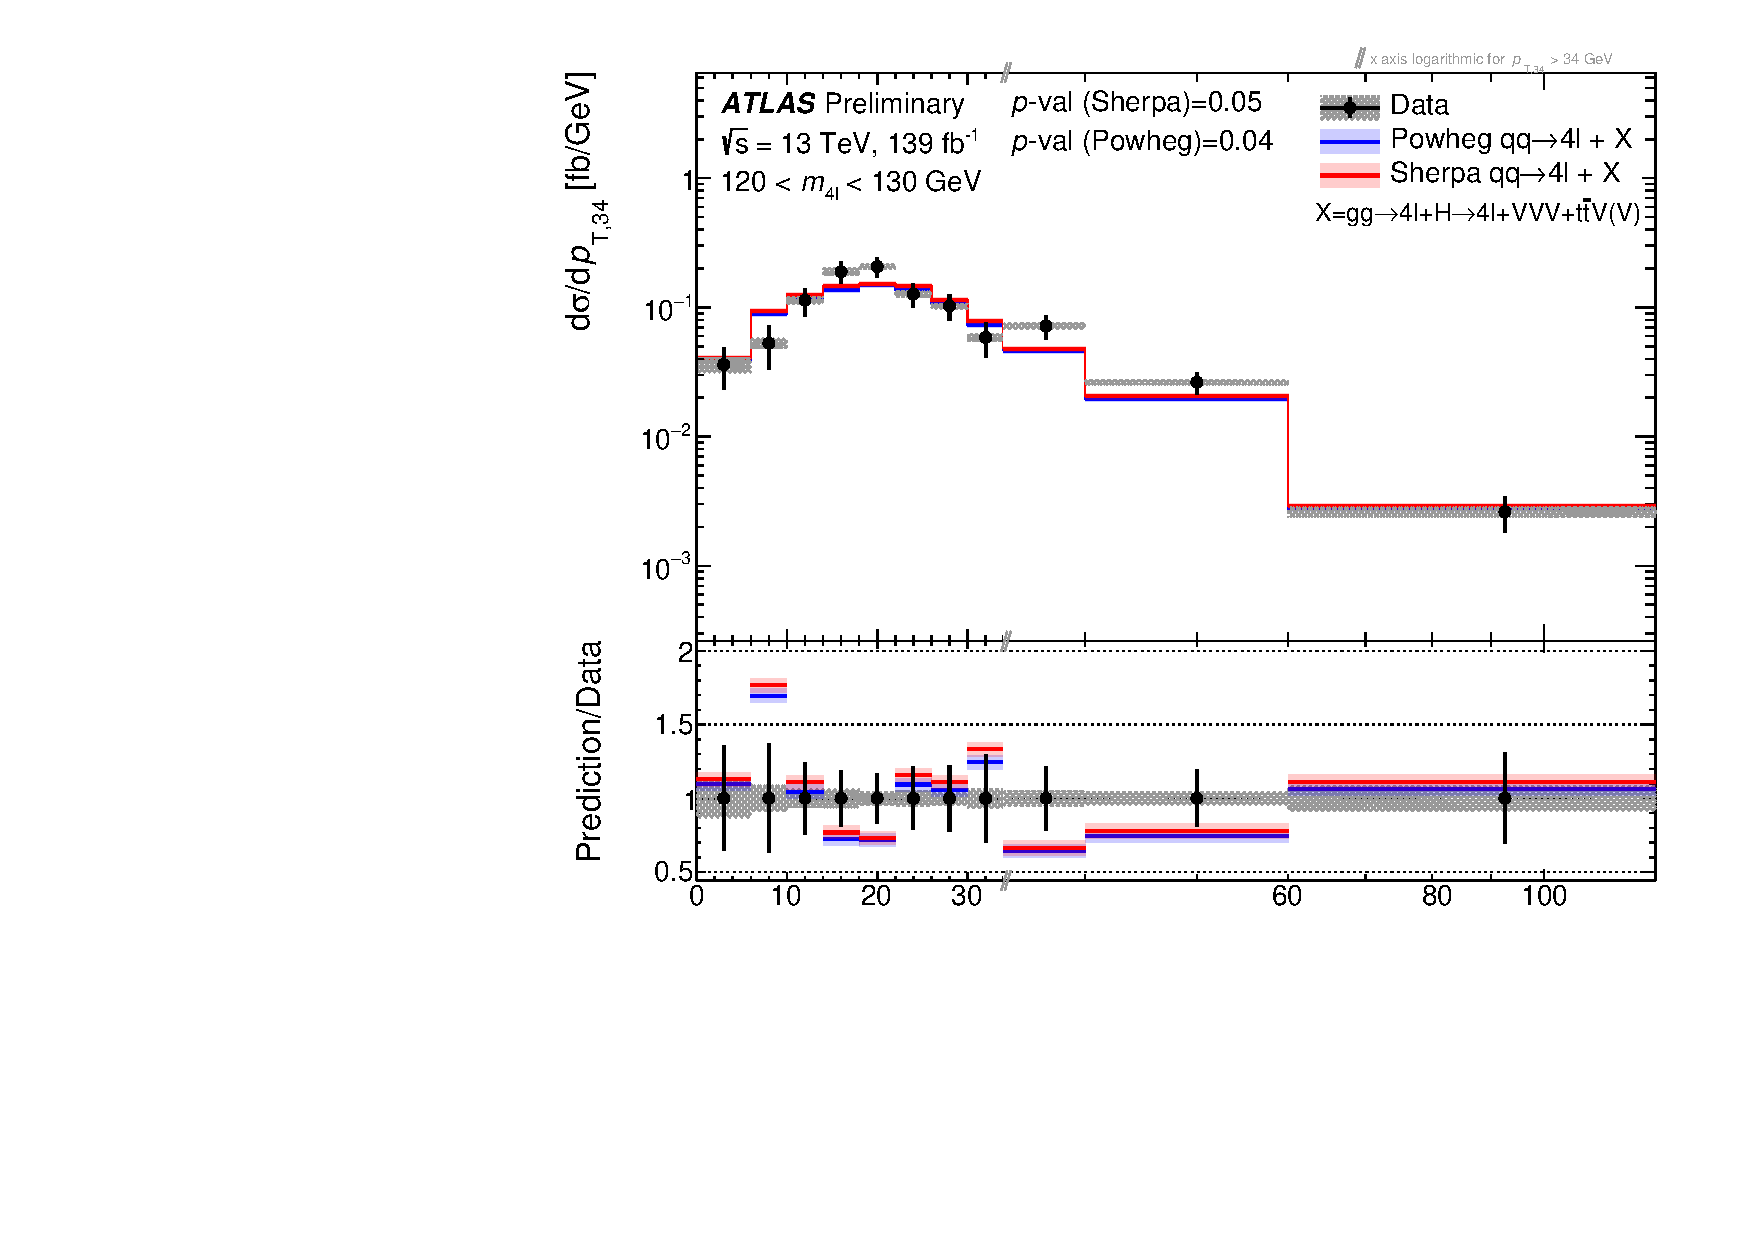
\includegraphics[width=.99\linewidth]{Figures/m4l/UnfoldedResults/linlog_Unfolded_Data_pt34_m4l120-130.pdf} \caption{\HFourL \ region}\label{fig:sub-second}
    \end{subfigure}
    \begin{subfigure}{.49\textwidth}\centering
      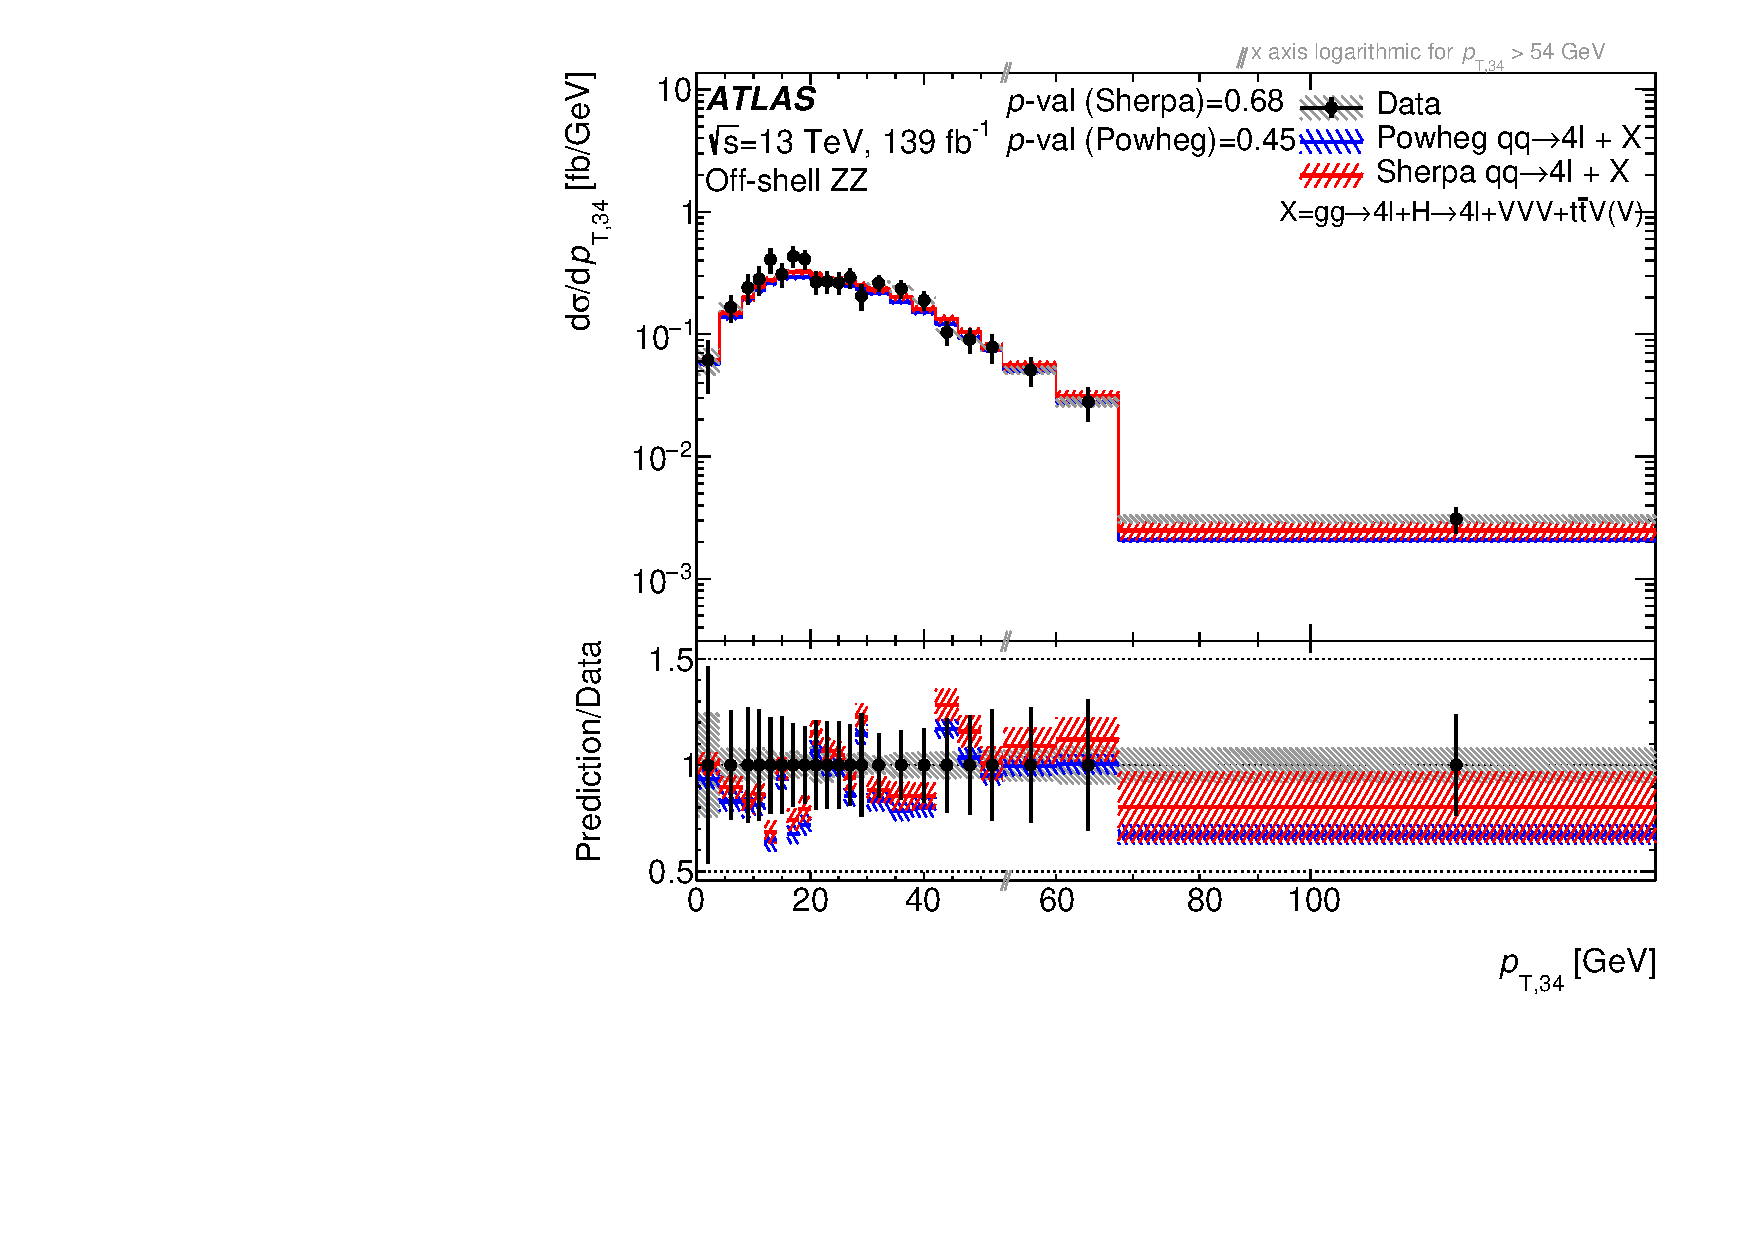
\includegraphics[width=.99\linewidth]{Figures/m4l/UnfoldedResults/linlog_Unfolded_Data_pt34_m4loffshell.pdf}  \caption{Off-shell $\Z\Z$ region}\label{fig:sub-third}
    \end{subfigure}
    \begin{subfigure}{.49\textwidth}\centering
      \includegraphics[width=.99\linewidth]{Figures/m4l/UnfoldedResults/linlog_Unfolded_Data_pt34_m4l180-2000.pdf}  \caption{On-shell $\Z\Z$ region}\label{fig:sub-fourth}
    \end{subfigure}
    \caption{Differential cross-section as a function of \ptZTwo{} in the four
        \mFourL{} regions. The measured data (black points) are  compared with the SM prediction using either \SHERPA{} (red, with red hashed band for the uncertainty) or \POWHEG{} + \pythia{} (blue, with blue hashed band for the uncertainty) to model the \qqFourL{} contribution. The error bars on the data points give the total uncertainty and the grey hashed band gives the systematic uncertainty. \Pvalue{} The  lower panel shows the ratio of the SM predictions to the data.}
    \label{fig:pt23_m4l}
\end{figure}

%% cosThetaStar1 vs m4l
\begin{figure}[htb!]
    \begin{subfigure}{.49\textwidth}\centering
      \includegraphics[width=.99\linewidth]{Figures/m4l/UnfoldedResults/linY_Unfolded_Data_cosThetaStar1_m4l60-100.pdf}\caption{\ZFourL \ region}\label{fig:sub-first}
    \end{subfigure}
    \begin{subfigure}{.49\textwidth}\centering
      \includegraphics[width=.99\linewidth]{Figures/m4l/UnfoldedResults/linY_Unfolded_Data_cosThetaStar1_m4l120-130.pdf} \caption{\HFourL \ region}\label{fig:sub-second}
    \end{subfigure}
    \begin{subfigure}{.49\textwidth}\centering
      \includegraphics[width=.99\linewidth]{Figures/m4l/UnfoldedResults/linY_Unfolded_Data_cosThetaStar1_m4loffshell.pdf}  \caption{Off-shell $\Z\Z$ region}\label{fig:sub-third}
    \end{subfigure}
    \begin{subfigure}{.49\textwidth}\centering
      \includegraphics[width=.99\linewidth]{Figures/m4l/UnfoldedResults/linY_Unfolded_Data_cosThetaStar1_m4l180-2000.pdf}  \caption{On-shell $\Z\Z$ region}\label{fig:sub-fourth}
    \end{subfigure}
    \caption{Differential cross-section as a function of \CTSOneTwo{} in the four
        \mFourL{} regions. The measured data (black points) are  compared with the SM prediction using either \SHERPA{} (red, with red hashed band for the uncertainty) or \POWHEG{} + \pythia{} (blue, with blue hashed band for the uncertainty) to model the \qqFourL{} contribution. The error bars on the data points give the total uncertainty and the grey hashed band gives the systematic uncertainty. \Pvalue{} The  lower panel shows the ratio of the SM predictions to the data.}
    \label{fig:cts12_m4l}
\end{figure}

%% cosThetaStar3 vs m4l
\begin{figure}[htb!]
    \begin{subfigure}{.49\textwidth}\centering
      \includegraphics[width=.99\linewidth]{Figures/m4l/UnfoldedResults/linY_Unfolded_Data_cosThetaStar3_m4l60-100.pdf}\caption{\ZFourL \ region}\label{fig:sub-first}
    \end{subfigure}
    \begin{subfigure}{.49\textwidth}\centering
      \includegraphics[width=.99\linewidth]{Figures/m4l/UnfoldedResults/linY_Unfolded_Data_cosThetaStar3_m4l120-130.pdf} \caption{\HFourL \ region}\label{fig:sub-second}
    \end{subfigure}
    \begin{subfigure}{.49\textwidth}\centering
      \includegraphics[width=.99\linewidth]{Figures/m4l/UnfoldedResults/linY_Unfolded_Data_cosThetaStar3_m4loffshell.pdf}  \caption{Off-shell $\Z\Z$ region}\label{fig:sub-third}
    \end{subfigure}
    \begin{subfigure}{.49\textwidth}\centering
      \includegraphics[width=.99\linewidth]{Figures/m4l/UnfoldedResults/linY_Unfolded_Data_cosThetaStar3_m4l180-2000.pdf}  \caption{On-shell $\Z\Z$ region}\label{fig:sub-fourth}
    \end{subfigure}
    \caption{Differential cross-section as a function of \CTSThreeFour{} in the four
        \mFourL{} regions. The measured data (black points) are  compared with the SM prediction using either \SHERPA{} (red, with red hashed band for the uncertainty) or \POWHEG{} + \pythia{} (blue, with blue hashed band for the uncertainty) to model the \qqFourL{} contribution. The error bars on the data points give the total uncertainty and the grey hashed band gives the systematic uncertainty. \Pvalue{} The  lower panel shows the ratio of the SM predictions to the data.}
    \label{fig:cts34_m4l}
\end{figure}

%% deltaPhiLeptons vs m4l
\begin{figure}[htb!]
    \begin{subfigure}{.49\textwidth}\centering
      \includegraphics[width=.99\linewidth]{Figures/m4l/UnfoldedResults/Unfolded_Data_deltaPhiLeadingLeptons_m4l60-100.pdf}\caption{\ZFourL \ region}\label{fig:sub-first}
    \end{subfigure}
    \begin{subfigure}{.49\textwidth}\centering
      \includegraphics[width=.99\linewidth]{Figures/m4l/UnfoldedResults/Unfolded_Data_deltaPhiLeadingLeptons_m4l120-130.pdf} \caption{\HFourL \ region}\label{fig:sub-second}
    \end{subfigure}
    \begin{subfigure}{.49\textwidth}\centering
      \includegraphics[width=.99\linewidth]{Figures/m4l/UnfoldedResults/Unfolded_Data_deltaPhiLeadingLeptons_m4loffshell.pdf}  \caption{Off-shell $\Z\Z$ region}\label{fig:sub-third}
    \end{subfigure}
    \begin{subfigure}{.49\textwidth}\centering
      \includegraphics[width=.99\linewidth]{Figures/m4l/UnfoldedResults/Unfolded_Data_deltaPhiLeadingLeptons_m4l180-2000.pdf}  \caption{On-shell $\Z\Z$ region}\label{fig:sub-fourth}
    \end{subfigure}
    \caption{Differential cross-section as a function of \dPhill{} in the four
        \mFourL{} regions. The measured data (black points) are  compared with the SM prediction using either \SHERPA{} (red, with red hashed band for the uncertainty) or \POWHEG{} + \pythia{} (blue, with blue hashed band for the uncertainty) to model the \qqFourL{} contribution. The error bars on the data points give the total uncertainty and the grey hashed band gives the systematic uncertainty. \Pvalue{} The  lower panel shows the ratio of the SM predictions to the data.}
    \label{fig:dPhill_m4l}
\end{figure}

%% deltaPhiPairs vs m4l
\begin{figure}[htb!]
    \begin{subfigure}{.49\textwidth}\centering
      \includegraphics[width=.99\linewidth]{Figures/m4l/UnfoldedResults/Unfolded_Data_deltaPhiPairs_m4l60-100.pdf}\caption{\ZFourL \ region}\label{fig:sub-first}
    \end{subfigure}
    \begin{subfigure}{.49\textwidth}\centering
      \includegraphics[width=.99\linewidth]{Figures/m4l/UnfoldedResults/Unfolded_Data_deltaPhiPairs_m4l120-130.pdf} \caption{\HFourL \ region}\label{fig:sub-second}
    \end{subfigure}
    \begin{subfigure}{.49\textwidth}\centering
      \includegraphics[width=.99\linewidth]{Figures/m4l/UnfoldedResults/Unfolded_Data_deltaPhiPairs_m4loffshell.pdf}  \caption{Off-shell $\Z\Z$ region}\label{fig:sub-third}
    \end{subfigure}
    \begin{subfigure}{.49\textwidth}\centering
      \includegraphics[width=.99\linewidth]{Figures/m4l/UnfoldedResults/Unfolded_Data_deltaPhiPairs_m4l180-2000.pdf}  \caption{On-shell $\Z\Z$ region}\label{fig:sub-fourth}
    \end{subfigure}
    \caption{Differential cross-section as a function of \dPhiPairs{} in the four
        \mFourL{} regions. The measured data (black points) are  compared with the SM prediction using either \SHERPA{} (red, with red hashed band for the uncertainty) or \POWHEG{} + \pythia{} (blue, with blue hashed band for the uncertainty) to model the \qqFourL{} contribution. The error bars on the data points give the total uncertainty and the grey hashed band gives the systematic uncertainty. \Pvalue{} The  lower panel shows the ratio of the SM predictions to the data.}
    \label{fig:dPhiPairs_m4l}
\end{figure}

%% deltaYPairs vs m4l
\begin{figure}[htb!]
    \begin{subfigure}{.49\textwidth}\centering
      \includegraphics[width=.99\linewidth]{Figures/m4l/UnfoldedResults/linY_Unfolded_Data_deltaYPairs_m4l60-100.pdf}\caption{\ZFourL \ region}\label{fig:sub-first}
    \end{subfigure}
    \begin{subfigure}{.49\textwidth}\centering
      \includegraphics[width=.99\linewidth]{Figures/m4l/UnfoldedResults/linY_Unfolded_Data_deltaYPairs_m4l120-130.pdf} \caption{\HFourL \ region}\label{fig:sub-second}
    \end{subfigure}
    \begin{subfigure}{.49\textwidth}\centering
      \includegraphics[width=.99\linewidth]{Figures/m4l/UnfoldedResults/linY_Unfolded_Data_deltaYPairs_m4loffshell.pdf}  \caption{Off-shell $\Z\Z$ region}\label{fig:sub-third}
    \end{subfigure}
    \begin{subfigure}{.49\textwidth}\centering
      \includegraphics[width=.99\linewidth]{Figures/m4l/UnfoldedResults/linY_Unfolded_Data_deltaYPairs_m4l180-2000.pdf}  \caption{On-shell $\Z\Z$ region}\label{fig:sub-fourth}
    \end{subfigure}
    \caption{Differential cross-section as a function of \dYPairs{} in the four
        \mFourL{} regions. The measured data (black points) are  compared with the SM prediction using either \SHERPA{} (red, with red hashed band for the uncertainty) or \POWHEG{} + \pythia{} (blue, with blue hashed band for the uncertainty) to model the \qqFourL{} contribution. The error bars on the data points give the total uncertainty and the grey hashed band gives the systematic uncertainty. \Pvalue{} The  lower panel shows the ratio of the SM predictions to the data.}
    \label{fig:dYPairs_m4l}
\end{figure}
 %% m4l vs pt4l
\begin{figure}[H]
    \begin{subfigure}{.46\textwidth}\centering
      \includegraphics[width=.95\linewidth]{Figures/m4l/UnfoldedResults/linlog_Unfolded_Data_m4l_pt4l0-10.pdf}\caption{$\unit{0}{\GeV} <  \ptFourL  < \unit{10}{\GeV}$}\label{fig:sub-first}
    \end{subfigure}
    \begin{subfigure}{.46\textwidth}\centering
      \includegraphics[width=.95\linewidth]{Figures/m4l/UnfoldedResults/linlog_Unfolded_Data_m4l_pt4l10-20.pdf} \caption{$\unit{10}{\GeV} <  \ptFourL  < \unit{20}{\GeV}$}\label{fig:sub-second}
    \end{subfigure}
    \begin{subfigure}{.46\textwidth}\centering
      \includegraphics[width=.95\linewidth]{Figures/m4l/UnfoldedResults/linlog_Unfolded_Data_m4l_pt4l20-50.pdf}  \caption{$\unit{20}{\GeV} <  \ptFourL  < \unit{50}{\GeV}$}\label{fig:sub-third}
    \end{subfigure}
    \begin{subfigure}{.46\textwidth}\centering
      \includegraphics[width=.95\linewidth]{Figures/m4l/UnfoldedResults/linlog_Unfolded_Data_m4l_pt4l50-100.pdf}  \caption{$\unit{50}{\GeV} <  \ptFourL  < \unit{100}{\GeV}$}\label{fig:sub-fourth}
    \end{subfigure}
        \begin{subfigure}{.46\textwidth}\centering
      \includegraphics[width=.95\linewidth]{Figures/m4l/UnfoldedResults/linlog_Unfolded_Data_m4l_pt4l100-600.pdf}  \caption{$\unit{100}{\GeV} <  \ptFourL  < \unit{60 0}{\GeV}$}\label{fig:sub-fifth}
    \end{subfigure}
    \caption{Differential cross-section as a function of \mFourL{} in slices of \ptFourL{}. \errorbars{} \SMpredictions{} \Pvalue{} The ratio of the \SHERPA{} prediction to the data is shown in the lower panel.}
    \label{fig:m4l_pt4l}
\end{figure}

%% m4l vs y4l
\begin{figure}[H]
    \begin{subfigure}{.46\textwidth}\centering
      \includegraphics[width=.95\linewidth]{Figures/m4l/UnfoldedResults/linlog_Unfolded_Data_m4l_y4l0-0dot3.pdf}\caption{0 < \yFourL{} < 0.3}\label{fig:sub-first}
    \end{subfigure}
    \begin{subfigure}{.46\textwidth}\centering
      \includegraphics[width=.95\linewidth]{Figures/m4l/UnfoldedResults/linlog_Unfolded_Data_m4l_y4l0dot3-0dot6.pdf} \caption{0.3 < \yFourL{} < 0.6}\label{fig:sub-second}
    \end{subfigure}
    \begin{subfigure}{.46\textwidth}\centering
      \includegraphics[width=.95\linewidth]{Figures/m4l/UnfoldedResults/linlog_Unfolded_Data_m4l_y4l0dot6-0dot9.pdf}  \caption{0.6 < \yFourL{} < 0.9}\label{fig:sub-third}
    \end{subfigure}
    \begin{subfigure}{.46\textwidth}\centering
      \includegraphics[width=.95\linewidth]{Figures/m4l/UnfoldedResults/linlog_Unfolded_Data_m4l_y4l0dot9-1dot2.pdf}  \caption{0.9 < \yFourL{} < 1.2}\label{fig:sub-fourth}
    \end{subfigure}
        \begin{subfigure}{.46\textwidth}\centering
      \includegraphics[width=.95\linewidth]{Figures/m4l/UnfoldedResults/linlog_Unfolded_Data_m4l_y4l1dot2-2dot5.pdf}  \caption{1.2 < \yFourL{} < 2.5}\label{fig:sub-fifth}
    \end{subfigure}
    \caption{Differential cross-section as a function of \mFourL{} in slices of \yFourL{}. \errorbars{} \SMpredictions{} \Pvalue{} The ratio of the \SHERPA{} prediction to the data is shown in the lower panel.}
    \label{fig:m4l_y4l}
\end{figure}

%% m4l vs flavour
\begin{figure}[H]
    \begin{subfigure}{.49\textwidth}\centering
      \includegraphics[width=.95\linewidth]{Figures/m4l/UnfoldedResults/linlog_Unfolded_Data_m4l_event_type4mu.pdf}\caption{$4\mu$ channel}\label{fig:sub-first}
    \end{subfigure}
    \begin{subfigure}{.49\textwidth}\centering
      \includegraphics[width=.95\linewidth]{Figures/m4l/UnfoldedResults/linlog_Unfolded_Data_m4l_event_type4e.pdf} \caption{$4e$ channel}\label{fig:sub-second}
    \end{subfigure}
    \begin{subfigure}{.49\textwidth}\centering
      \includegraphics[width=.95\linewidth]{Figures/m4l/UnfoldedResults/linlog_Unfolded_Data_m4l_event_type2mu2e.pdf}  \caption{$2e2\mu$ channel}\label{fig:sub-third}
    \end{subfigure}
    \caption{Differential cross-section as a function of \mFourL{} for each lepton flavour channel. \errorbars{} \SMpredictions{} \Pvalue{} The ratio of the \SHERPA{} prediction to the data is shown in the lower panel. The $x$-axis is on a linear scale until $\mFourL = 225$~\GeV, where it switches to a logarithmic scale.}
    \label{fig:m4l_flavour}
\end{figure}

%% m12 vs m4l
\begin{figure}[H]
    \begin{subfigure}{.49\textwidth}\centering
      \includegraphics[width=.95\linewidth]{Figures/m4l/UnfoldedResults/linY_Unfolded_Data_m12_m4l60-100.pdf}  
      \caption{\ZFourL \ region}
      \label{fig:sub-first}
    \end{subfigure}
    \begin{subfigure}{.49\textwidth}\centering
      \includegraphics[width=.95\linewidth]{Figures/m4l/UnfoldedResults/higgs_Unfolded_Data_m12_m4l120-130.pdf}  
      \caption{\HFourL \ region}
      \label{fig:sub-second}
    \end{subfigure}
    \begin{subfigure}{.49\textwidth}
      \centering
      \includegraphics[width=.95\linewidth]{Figures/m4l/UnfoldedResults/Unfolded_Data_m12_m4loffshell.pdf}  
      \caption{Off-shell $\Z\Z$ region}
      \label{fig:sub-third}
    \end{subfigure}
    \begin{subfigure}{.49\textwidth}
      \centering
      \includegraphics[width=.95\linewidth]{Figures/m4l/UnfoldedResults/Unfolded_Data_m12_m4l180-2000.pdf}  
      \caption{On-shell $\Z\Z$ region}
      \label{fig:sub-fourth}
    \end{subfigure}
    \caption{Differential cross-section as a function of \mZOne{} in the four
        \mFourL{} regions. \errorbars{} \SMpredictions{} \Pvalue{} The ratio of the \SHERPA{} prediction to the data is shown in the lower panel. In (b) the contribution from Higgs production is shown in addition to the total SM prediction.}
    \label{fig:m12_m4l}
\end{figure}
%% m34 vs m4l
\begin{figure}[H]
    \begin{subfigure}{.49\textwidth}\centering
      \includegraphics[width=.95\linewidth]{Figures/m4l/UnfoldedResults/linY_Unfolded_Data_m34_m4l60-100.pdf}\caption{\ZFourL \ region}\label{fig:sub-first}
    \end{subfigure}
    \begin{subfigure}{.49\textwidth}\centering
      \includegraphics[width=.95\linewidth]{Figures/m4l/UnfoldedResults/higgs_linY_Unfolded_Data_m34_m4l120-130.pdf} \caption{\HFourL \ region}\label{fig:sub-second}
    \end{subfigure}
    \begin{subfigure}{.49\textwidth}\centering
      \includegraphics[width=.95\linewidth]{Figures/m4l/UnfoldedResults/linY_Unfolded_Data_m34_m4loffshell.pdf}  \caption{Off-shell $\Z\Z$ region}\label{fig:sub-third}
    \end{subfigure}
    \begin{subfigure}{.49\textwidth}\centering
      \includegraphics[width=.95\linewidth]{Figures/m4l/UnfoldedResults/Unfolded_Data_m34_m4l180-2000.pdf}  \caption{On-shell $\Z\Z$ region}\label{fig:sub-fourth}
    \end{subfigure}
    \caption{Differential cross-section as a function of \mZTwo{} in the four
        \mFourL{} regions. The measured data (black points) are  compared with the SM prediction using either \SHERPA{} (red, with red hashed band for the uncertainty) or \POWHEG{} + \pythia{} (blue, with blue hashed band for the uncertainty) to model the \qqFourL{} contribution. In (b) the contribution from Higgs production is shown in addition to the total SM prediction. The error bars on the data points give the total uncertainty and the grey hashed band gives the systematic uncertainty. \Pvalue{} The  lower panel shows the ratio of the SM predictions to the data.}
    \label{fig:m34_m4l}
\end{figure}

%% pt12 vs m4l
\begin{figure}[H]
    \begin{subfigure}{.49\textwidth}\centering
      \includegraphics[width=.95\linewidth]{Figures/m4l/UnfoldedResults/linlog_Unfolded_Data_pt12_m4l60-100.pdf}\caption{\ZFourL \ region}\label{fig:sub-first}
    \end{subfigure}
    \begin{subfigure}{.49\textwidth}\centering
      \includegraphics[width=.95\linewidth]{Figures/m4l/UnfoldedResults/linlog_Unfolded_Data_pt12_m4l120-130.pdf} \caption{\HFourL \ region}\label{fig:sub-second}
    \end{subfigure}
    \begin{subfigure}{.49\textwidth}\centering
      \includegraphics[width=.95\linewidth]{Figures/m4l/UnfoldedResults/linlog_Unfolded_Data_pt12_m4loffshell.pdf}  \caption{Off-shell $\Z\Z$ region}\label{fig:sub-third}
    \end{subfigure}
    \begin{subfigure}{.49\textwidth}\centering
      \includegraphics[width=.95\linewidth]{Figures/m4l/UnfoldedResults/linlog_Unfolded_Data_pt12_m4l180-2000.pdf}  \caption{On-shell $\Z\Z$ region}\label{fig:sub-fourth}
    \end{subfigure}
    \caption{Differential cross-section as a function of \ptZOne{} in the four
        \mFourL{} regions. The measured data (black points) are  compared with the SM prediction using either \SHERPA{} (red, with red hashed band for the uncertainty) or \POWHEG{} + \pythia{} (blue, with blue hashed band for the uncertainty) to model the \qqFourL{} contribution. In (b) the contribution from Higgs production is shown in addition to the total SM prediction. The error bars on the data points give the total uncertainty and the grey hashed band gives the systematic uncertainty. \Pvalue{} The  lower panel shows the ratio of the SM predictions to the data.}
    \label{fig:pt12_m4l}
\end{figure}

%% pt34 vs m4l
\begin{figure}[H]
    \begin{subfigure}{.49\textwidth}\centering
      \includegraphics[width=.95\linewidth]{Figures/m4l/UnfoldedResults/linlog_Unfolded_Data_pt34_m4l60-100.pdf}\caption{\ZFourL \ region}\label{fig:sub-first}
    \end{subfigure}
    \begin{subfigure}{.49\textwidth}\centering
      \includegraphics[width=.95\linewidth]{Figures/m4l/UnfoldedResults/linlog_Unfolded_Data_pt34_m4l120-130.pdf} \caption{\HFourL \ region}\label{fig:sub-second}
    \end{subfigure}
    \begin{subfigure}{.49\textwidth}\centering
      \includegraphics[width=.95\linewidth]{Figures/m4l/UnfoldedResults/linlog_Unfolded_Data_pt34_m4loffshell.pdf}  \caption{Off-shell $\Z\Z$ region}\label{fig:sub-third}
    \end{subfigure}
    \begin{subfigure}{.49\textwidth}\centering
      \includegraphics[width=.95\linewidth]{Figures/m4l/UnfoldedResults/linlog_Unfolded_Data_pt34_m4l180-2000.pdf}  \caption{On-shell $\Z\Z$ region}\label{fig:sub-fourth}
    \end{subfigure}
    \caption{Differential cross-section as a function of \ptZTwo{} in the four
        \mFourL{} regions. The measured data (black points) are  compared with the SM prediction using either \SHERPA{} (red, with red hashed band for the uncertainty) or \POWHEG{} + \pythia{} (blue, with blue hashed band for the uncertainty) to model the \qqFourL{} contribution. The error bars on the data points give the total uncertainty and the grey hashed band gives the systematic uncertainty. \Pvalue{} The  lower panel shows the ratio of the SM predictions to the data.}
    \label{fig:pt34_m4l}
\end{figure}

%% cosThetaStar1 vs m4l
\begin{figure}[H]
    \begin{subfigure}{.49\textwidth}\centering
      \includegraphics[width=.95\linewidth]{Figures/m4l/UnfoldedResults/linY_Unfolded_Data_cosThetaStar1_m4l60-100.pdf}\caption{\ZFourL \ region}\label{fig:sub-first}
    \end{subfigure}
    \begin{subfigure}{.49\textwidth}\centering
      \includegraphics[width=.95\linewidth]{Figures/m4l/UnfoldedResults/linY_Unfolded_Data_cosThetaStar1_m4l120-130.pdf} \caption{\HFourL \ region}\label{fig:sub-second}
    \end{subfigure}
    \begin{subfigure}{.49\textwidth}\centering
      \includegraphics[width=.95\linewidth]{Figures/m4l/UnfoldedResults/linY_Unfolded_Data_cosThetaStar1_m4loffshell.pdf}  \caption{Off-shell $\Z\Z$ region}\label{fig:sub-third}
    \end{subfigure}
    \begin{subfigure}{.49\textwidth}\centering
      \includegraphics[width=.95\linewidth]{Figures/m4l/UnfoldedResults/linY_Unfolded_Data_cosThetaStar1_m4l180-2000.pdf}  \caption{On-shell $\Z\Z$ region}\label{fig:sub-fourth}
    \end{subfigure}
    \caption{Differential cross-section as a function of \CTSOneTwo{} in the four
        \mFourL{} regions. The measured data (black points) are  compared with the SM prediction using either \SHERPA{} (red, with red hashed band for the uncertainty) or \POWHEG{} + \pythia{} (blue, with blue hashed band for the uncertainty) to model the \qqFourL{} contribution. The error bars on the data points give the total uncertainty and the grey hashed band gives the systematic uncertainty. \Pvalue{} The  lower panel shows the ratio of the SM predictions to the data.}
    \label{fig:cts12_m4l}
\end{figure}

%% cosThetaStar3 vs m4l
\begin{figure}[H]
    \begin{subfigure}{.49\textwidth}\centering
      \includegraphics[width=.95\linewidth]{Figures/m4l/UnfoldedResults/linY_Unfolded_Data_cosThetaStar3_m4l60-100.pdf}\caption{\ZFourL \ region}\label{fig:sub-first}
    \end{subfigure}
    \begin{subfigure}{.49\textwidth}\centering
      \includegraphics[width=.95\linewidth]{Figures/m4l/UnfoldedResults/linY_Unfolded_Data_cosThetaStar3_m4l120-130.pdf} \caption{\HFourL \ region}\label{fig:sub-second}
    \end{subfigure}
    \begin{subfigure}{.49\textwidth}\centering
      \includegraphics[width=.95\linewidth]{Figures/m4l/UnfoldedResults/linY_Unfolded_Data_cosThetaStar3_m4loffshell.pdf}  \caption{Off-shell $\Z\Z$ region}\label{fig:sub-third}
    \end{subfigure}
    \begin{subfigure}{.49\textwidth}\centering
      \includegraphics[width=.95\linewidth]{Figures/m4l/UnfoldedResults/linY_Unfolded_Data_cosThetaStar3_m4l180-2000.pdf}  \caption{On-shell $\Z\Z$ region}\label{fig:sub-fourth}
    \end{subfigure}
    \caption{Differential cross-section as a function of \CTSThreeFour{} in the four
        \mFourL{} regions. The measured data (black points) are  compared with the SM prediction using either \SHERPA{} (red, with red hashed band for the uncertainty) or \POWHEG{} + \pythia{} (blue, with blue hashed band for the uncertainty) to model the \qqFourL{} contribution. The error bars on the data points give the total uncertainty and the grey hashed band gives the systematic uncertainty. \Pvalue{} The  lower panel shows the ratio of the SM predictions to the data.}
    \label{fig:cts34_m4l}
\end{figure}

%% deltaPhiLeptons vs m4l
\begin{figure}[H]
    \begin{subfigure}{.49\textwidth}\centering
      \includegraphics[width=.95\linewidth]{Figures/m4l/UnfoldedResults/Unfolded_Data_deltaPhiLeadingLeptons_m4l60-100.pdf}\caption{\ZFourL \ region}\label{fig:sub-first}
    \end{subfigure}
    \begin{subfigure}{.49\textwidth}\centering
      \includegraphics[width=.95\linewidth]{Figures/m4l/UnfoldedResults/Unfolded_Data_deltaPhiLeadingLeptons_m4l120-130.pdf} \caption{\HFourL \ region}\label{fig:sub-second}
    \end{subfigure}
    \begin{subfigure}{.49\textwidth}\centering
      \includegraphics[width=.95\linewidth]{Figures/m4l/UnfoldedResults/Unfolded_Data_deltaPhiLeadingLeptons_m4loffshell.pdf}  \caption{Off-shell $\Z\Z$ region}\label{fig:sub-third}
    \end{subfigure}
    \begin{subfigure}{.49\textwidth}\centering
      \includegraphics[width=.95\linewidth]{Figures/m4l/UnfoldedResults/Unfolded_Data_deltaPhiLeadingLeptons_m4l180-2000.pdf}  \caption{On-shell $\Z\Z$ region}\label{fig:sub-fourth}
    \end{subfigure}
    \caption{Differential cross-section as a function of \dPhill{} in the four
        \mFourL{} regions. The measured data (black points) are  compared with the SM prediction using either \SHERPA{} (red, with red hashed band for the uncertainty) or \POWHEG{} + \pythia{} (blue, with blue hashed band for the uncertainty) to model the \qqFourL{} contribution. The error bars on the data points give the total uncertainty and the grey hashed band gives the systematic uncertainty. \Pvalue{} The  lower panel shows the ratio of the SM predictions to the data.}
    \label{fig:dPhill_m4l}
\end{figure}

%% deltaPhiPairs vs m4l
\begin{figure}[H]
    \begin{subfigure}{.49\textwidth}\centering
      \includegraphics[width=.95\linewidth]{Figures/m4l/UnfoldedResults/Unfolded_Data_deltaPhiPairs_m4l60-100.pdf}\caption{\ZFourL \ region}\label{fig:sub-first}
    \end{subfigure}
    \begin{subfigure}{.49\textwidth}\centering
      \includegraphics[width=.95\linewidth]{Figures/m4l/UnfoldedResults/Unfolded_Data_deltaPhiPairs_m4l120-130.pdf} \caption{\HFourL \ region}\label{fig:sub-second}
    \end{subfigure}
    \begin{subfigure}{.49\textwidth}\centering
      \includegraphics[width=.95\linewidth]{Figures/m4l/UnfoldedResults/Unfolded_Data_deltaPhiPairs_m4loffshell.pdf}  \caption{Off-shell $\Z\Z$ region}\label{fig:sub-third}
    \end{subfigure}
    \begin{subfigure}{.49\textwidth}\centering
      \includegraphics[width=.95\linewidth]{Figures/m4l/UnfoldedResults/Unfolded_Data_deltaPhiPairs_m4l180-2000.pdf}  \caption{On-shell $\Z\Z$ region}\label{fig:sub-fourth}
    \end{subfigure}
    \caption{Differential cross-section as a function of \dPhiPairs{} in the four
        \mFourL{} regions. The measured data (black points) are  compared with the SM prediction using either \SHERPA{} (red, with red hashed band for the uncertainty) or \POWHEG{} + \pythia{} (blue, with blue hashed band for the uncertainty) to model the \qqFourL{} contribution. The error bars on the data points give the total uncertainty and the grey hashed band gives the systematic uncertainty. \Pvalue{} The  lower panel shows the ratio of the SM predictions to the data.}
    \label{fig:dPhiPairs_m4l}
\end{figure}

%% deltaYPairs vs m4l
\begin{figure}[H]
    \begin{subfigure}{.49\textwidth}\centering
      \includegraphics[width=.95\linewidth]{Figures/m4l/UnfoldedResults/linY_Unfolded_Data_deltaYPairs_m4l60-100.pdf}\caption{\ZFourL \ region}\label{fig:sub-first}
    \end{subfigure}
    \begin{subfigure}{.49\textwidth}\centering
      \includegraphics[width=.95\linewidth]{Figures/m4l/UnfoldedResults/linY_Unfolded_Data_deltaYPairs_m4l120-130.pdf} \caption{\HFourL \ region}\label{fig:sub-second}
    \end{subfigure}
    \begin{subfigure}{.49\textwidth}\centering
      \includegraphics[width=.95\linewidth]{Figures/m4l/UnfoldedResults/linY_Unfolded_Data_deltaYPairs_m4loffshell.pdf}  \caption{Off-shell $\Z\Z$ region}\label{fig:sub-third}
    \end{subfigure}
    \begin{subfigure}{.49\textwidth}\centering
      \includegraphics[width=.95\linewidth]{Figures/m4l/UnfoldedResults/linY_Unfolded_Data_deltaYPairs_m4l180-2000.pdf}  \caption{On-shell $\Z\Z$ region}\label{fig:sub-fourth}
    \end{subfigure}
    \caption{Differential cross-section as a function of \dYPairs{} in the four
        \mFourL{} regions. The measured data (black points) are  compared with the SM prediction using either \SHERPA{} (red, with red hashed band for the uncertainty) or \POWHEG{} + \pythia{} (blue, with blue hashed band for the uncertainty) to model the \qqFourL{} contribution. The error bars on the data points give the total uncertainty and the grey hashed band gives the systematic uncertainty. \Pvalue{} The  lower panel shows the ratio of the SM predictions to the data.}
    \label{fig:dYPairs_m4l}
\end{figure}
=======
%% m4l motivation
\section{Motivation for the \mFourL measurement}
\label{sec:fourlepmotivation}

The four lepton channel is a particularly interesting channel to study as it receives contributions from many physics processes.  

First and foremost, there is the production of a pair of \PZ-bosons via quark-antiquark interactions in \info[]{s-channel not in SM because it includes neutral ZZZ or ZZ\photon vertex} both the \Ptop- and \Pup-channel. The \Ptop-channel diagram is shown in Figure \ref{fig:m4lfeynman:qqZZ}, and represents, by far, \improvement[]{Read more about why the u-channel diagram is not preferred} the largest contribution to the \ZZ production and thus to the \mFourL distribution. At the low mass end where $\mFourL=m_{PZ}$, there is resonant production of a single \PZ boson via the s-channel diagram in Figure \ref{fig:m4lfeynman:singleZ}. At $\mFourL=\unit{180}{\GeV}$ and beyond, the threshold for the on-shell production of two \PZ bosons is reached and results in a peak in the four lepton invariant mass spectrum. 

Second in magnitude is the gluon-induced production of a \PZ boson pair. This occurs via a triangle or box quark loop, which results in a factor $\alpha_s^2$ suppression. It still plays a substantial role, however, because at small $x$\footnote{Here $x$ is the component of the proton's momentum carried by the struck quark. At the \LHC the protons have very high energies; therefore the \LHC can be described as a small $x$ collider \cite{zotov2012small}} gluon-gluon luminosity is higher than the quark-antiquark luminosity \cite{Glover:194539}. The contribution from this process in on the order of ten percent \cite{Becker:2230817}. Finally in the pool of \PZ boson pairs there is a small contribution from decaying Higgs bosons, which themselves are produced also via gluon fusion, as illustrated in Figure \ref{fig:m4lfeynman:ggHZZ}. There is resonant Higgs production at \mFourL=\unit{125}{\GeV}, and a non-resonant enhancement at $\mFourL=m_{\Ptop}=\unit{350}{\GeV}$ from the top quark loop. Beyond \unit{350}{\GeV}, the Higgs-mediated \PZ boson pair production process destructively interferes with continuum production of on-shell \PZ bosons \cite{Campbell_2016}.

The \mFourL distribution can be a useful probe for certain new physics scenarios. Take for example, the high mass tail of the invariant mass spectrum. This region is dependent on the couplings of the Higgs to incoming and outgoing particles while independent of the Higgs boson width \cite{Campbell_2016}, a unique property that can be exploited to derive model-independent limits on the Higgs couplings, and on the \todo{reword, this is copy pasted} contribution of new states in the Higgs to gluon coupling \cite{Cacciapaglia_2014}. It has also been previously exploited to derive model-independent constraints on the Higgs boson width \cite{Caola_2013}. 

%% Secondly, under specific assumptions a class of models exists for which the off-shell coupling measurement together with a measurement of the on-shell signal strength can be re-interpreted in terms of a bound on the total Higgs boson width. In this paper, we provide a first step towards a classification of the models for which a total width measurement is viable and we discuss examples of BSM models for which the off-shell coupling measurement can be important in either constraining or even discovering new physics in the upcoming LHC runs

\begin{figure}
    \centering
    \includegraphics[width=0.5\textwidth]{Figures/m4l/m4lbreakdown.png}
    \caption{Breakdown of contributing processes contributing to the \mFourL distribution.}
    \todo[inline]{Replace and remake with our miniTrees.}
    \label{fig:m4lbreakdown}
\end{figure}

\begin{figure}
\centering
\begin{subfigure}{.24\textwidth}
  \centering
  \includegraphics[width=.23\textwidth]{Figures/FeynGraphs/qqZZ4l.pdf}
  \caption{\qqZZ}
  \label{fig:m4lfeynman:qqZZ}
\end{subfigure}%
\begin{subfigure}{.24\textwidth}
  \centering
  \includegraphics[width=.23\textwidth]{Figures/FeynGraphs/qqZZ4lrad.pdf}
  \caption{A subfigure}
  \label{fig:m4lfeynman:singleZ}
\end{subfigure}
\begin{subfigure}{.24\textwidth}
  \centering
  \includegraphics[width=.23\textwidth]{Figures/FeynGraphs/ggZZ4lbox.pdf}
  \caption{A subfigure}
  \label{fig:m4lfeynman:ggZZ}
\end{subfigure}
\begin{subfigure}{.24\textwidth}
  \centering
  \includegraphics[width=.23\textwidth]{Figures/FeynGraphs/ggZZ4lhiggs.pdf}
  \caption{A subfigure}
  \label{fig:m4lfeynman:ggHZZ}
\end{subfigure}
\caption{Feynman diagrams for quark- and gluon-induced \ZZ production. The processes shown are the main contributors.}
\label{fig:m4lfeynman}
\end{figure}

% this channel provides a clean leptonic final state resulting in a small instrumental background, where one or more of the reconstructed lepton candidates originate from the misidentification of jet fragments or from nonprompt leptons.

%% Signal definition and event selection
\section{Signal and fiducial region definition}
\label{sec:signaldef}

The motivation behind this analysis is to make a measurement as inclusive and as model-independent as possible. Any process leading to a final state of four lepton - made up of two same flavour opposite sign electron or muon pairs - is considered to be part of the signal. Electrons or muons originating from fully leptonic decays of taus are counted towards the signal. 

The fiducial region definition follows closely the acceptance of the detector. Furthermore, by loosening the mass cuts, there is higher event acceptance especially in the low mass regions. Preliminary studies were conducted to investigate the impact of loosening and simplifying the dilepton lower mass cut to \unit{5}{\GeV} and removing the upper mass cut, for example, as opposed to the varying higher cuts in the previous round of the analysis. Unsurprisingly, these result in a higher event yield in both the low and high mass tails of the \mFourL distribution. 

The final state is defined solely in terms of final state particles as opposed to targeting a specific process. Beyond the requirement of two same flavour opposite sign lepton pairs, the measurement is inclusive to additional particles such as additional leptons, jets, and invisible particles. Previous irreducible backgrounds (\VVV, \ttZ) are now considered as part of the signal since they produce four or more prompt leptons.

\missingfigure{Emily plots for loosening mass cuts}

\subsection{Lepton definitions}

For particle physicists, a prompt lepton simply means the lepton did not originate from a hadron. Prompt leptons are further classified into three categories depending on their association with emitted photons. These three categories are:
\begin{itemize}
    \item Born leptons: leptons prior to QED Final State Radiation (FSR);
    \item Bare leptons: leptons after QED FSR;
    \item Dressed leptons: leptons after QED FSR, that then have the four momenta of nearby radiated photons added to it. 
\end{itemize}
The ATLAS detector makes lepton measurements after QED FSR has occurred. It is for this reason that born leptons are not the best choice. It is more realistic to perform measurements involving only final state particles, and objects constructed from final state particles, such as dressed leptons \cite{Kar:ab1be6}. 

\subsubsection{Dressed electrons and bare muons}

In this analysis, a choice of dressing electrons but leaving muons bare was made to closer mimic what is seen by the detector. 

%% Truth isolation
When selecting leptons in the data, there is a complex isolation criteria applied \todo[]{What is this isolation criteria?}. An emulation of this reconstruction-level criteria is included in the fiducial region definition. Although the particle-level application is a simplification, it nevertheless returns a result that is closer to what is actually measured. The particle-level truth isolation criteria requires the sum of the transverse momentum of all charged particles inside a $\Delta R  = 0.3$ cone of the lepton, divided by transverse momentum of the lepton itself, to be less than 0.16. If any other selected leptons are within the cone, their
momenta is not included. 
$$\dfrac{\pt(\Delta R  = 0.3)}{\pt(\text{lepton})}<0.16$$
\subsection{Fiducial region}

\begin{table}[bp]
  \begin{tabular}{lllll}
        & Lepton requirements \\
        \midrule
        Electrons & Dressed lepton definition\\
                & \pt > \unit{5}{\GeV}\\
                & $|\eta| < 2.47$\\
        Muons & Bare lepton definition\\
            & \pt > \unit{7}{\GeV}\\
            & $|\eta| < 2.7$\\
        \bottomrule
        \toprule
        & Event requirements \\
        \midrule
            Four-lepton signature & At least 4 leptons, with 2 Same-Flavour, Opposite-Sign pairs \\
               Lepton kinematics   &   $\pt > 20 / 10$~\GeV{} for
                                     leading two leptons \\ [0.3cm]
              Lepton separation               &   $\Delta R_{ij} > 0.05$ for any leptons \\
              $J/\psi$-Veto &    $  m_{ij} > 5$~\GeV for all SFOS pairs \\
              Truth isolation & ptcone30/\pt < 0.16 \\
  \end{tabular}
  \caption{Fiducial region definition.}
  \label{tab:fidregion}
\end{table}

\missingfigure[]{Dressed electrons, bare muons plot}

\subsection*{Lepton pairing and quadruplet formation} 
\todo[inline]{Reword this whole subsection!!}
Events satisfying the requirements described above enter the fiducial region of the measurement. 
In order to define observables, a unique set of exactly four leptons per event is chosen: 
\begin{itemize}
\item First, the SFOS lepton pair with an invariant mass closest to the Z boson mass is selected as the primary pair in the event. 
\item The remaining SFOS lepton pair closest to the Z boson mass is then referred to as the secondary pair, and completes the quadruplet. 
\end{itemize}
In this way, only one quadruplet is defined even in events containing more than four leptons.
This selection strategy is chosen since it prefers to form pairs that correspond to on-shell Z bosons for the dominant $ZZ$ pair production process, making the pair-level observables based on this definition comparable to such obtained in dedicated $ZZ$ production measurements. This is explored further in Appendix~\ref{app:pairing}. 
The pair and quadruplet formation does not have any impact on the event selection outcome. 

\section{Measured observables}

The star observable of the analysis is none other than the four lepton invariant mass, \mFourL. It has been measured previously by both the \ATLAS and the \CMS experiment \todo{missing citation} \cite{}. As with the previous round of the analysis, the \mFourL distribution is also measured double-differentially, in slices of the transverse momentum of the four lepton system, the absolute rapidity of the four lepton system, and the flavour channel of the four lepton system. 

New to this round of the analysis is the division of the four lepton invariant mass spectrum into four separate regions, each dominated by a different process. From \unit{60}{\GeV}-\unit{100}{\GeV} resonant single \Z production reigns, similarly the \unit{120}{\GeV}-\unit{130}{\GeV} region is dominated by Higgs production, and the high mass region from \unit{180}{\GeV}-\unit{2000}{\GeV} by on-shell \ZZ production. Lastly to fill the gaps between  \unit{20}{\GeV}-\unit{60}{\GeV}, \unit{100}{\GeV}-\unit{120}{\GeV}, and \unit{130}{\GeV}-\unit{180}{\GeV} is the off-shell \ZZ region. This is summarised in Table \ref{tab:m4lregions}. The following variables are measured double differentially in these four regions:

\begin{itemize}
    \item Cosine of angle $\theta^{*}$, where $\theta^{*}$ is the angle between the \todo{definitely check this} lepton in the rest frame and the \Z boson in the lab frame. This angle is sensitive to the polarisation of the decaying boson.
    \item The difference in rapidity between the lepton pairs
    \item The difference in azimuthal angle between the lepton pairs, and between leading leptons
    \item The invariant mass of the lepton pairs
    \item The transverse momentum of the lepton pairs
\end{itemize}

\begin{table}[bp]
  \begin{tabular}{lllll}
        Region & \mFourL interval(s) \\
        \midrule
        \ZFourL & \unit{60}{\GeV} < \mFourL < \unit{100}{\GeV} \\
        \HFourL & \unit{120}{\GeV} < \mFourL < \unit{130}{\GeV} \\
        On-shell \ZZ & \unit{180}{\GeV} < \mFourL < \unit{2000}{\GeV} \\
        Off-shell \ZZ & \unit{20}{\GeV} < \mFourL < \unit{60}{\GeV}, \unit{100}{\GeV} < \mFourL < \unit{120}{\GeV}, \\
          & and \unit{130}{\GeV} < \mFourL < \unit{180}{\GeV}\\
  \end{tabular}
  \caption{The four \mFourL regions dominated by the single \Z, Higgs, on-shell and off-shell \ZZ processes.}
  \label{tab:m4lregions}
\end{table}

\section{Event reconstruction and selection}
\label{sec:eventselection}
A critical aspect of any analysis is its event selection. The dominant backgrounds are shaped by the selection choices, and signal sensitivity are enhanced with optimized cuts. The objective of the selection in this analysis is to efficiently identify the four lepton final states while keeping the background at a minimum. This is achieved through a combination of online trigger (described in detail in Section \ref{ssec:ATLAStrigger}) and offline event selection cuts. As with all \ATLAS analysis, basic requirements on the event cleaning are imposed. Only data recorded with stable beam conditions and with all relevant information from sub-detectors present are considered. 

The requirements on event selection are outlined in Tables \ref{tab:baselineLeptons} and \ref{tab:signalLeptons}. The cuts are largely based on the fiducial region definition of Table~\ref{tab:fidregion} combined with the limited acceptance and efficiency of \ATLAS's object reconstruction. This ensures that there is little to no extrapolation into unmeasured regions on phase space when unfolding. 

First there is the selection of baseline electrons and muons. For both the Loose identification working point is used. For electrons there is a minimum requirement of $p_T>$\unit{7}{\GeV} and $|\eta|>2.7$. For muons it is $p_T>$\unit{5}{\GeV} and $|\eta|>2.47$, and if the muon is a calorimeter-tagged muon there is a more stringent $p_T>$\unit{15}{\GeV} requirement to account for their lower purity. The vertex association requirement ensures that the leptons are associated to the primary vertex in the event. Lastly a lepton-favoured overlap removal is applied to ensure that objects are reconstructed with some distance in between. In the event where a lepton and a jet overlap, priority is given to the lepton. The events that pass these criteria (listed in Table \ref{tab:baselineLeptons}) are classified as baseline leptons.

Additional lepton kinematic requirements are imposed on the leptons after overlap removal. The leading and sub-leading lepton must have a transverse momentum higher than \unit{20}{\GeV} and \unit{10}{\GeV} respectively. The minimum separation between leptons is set at $\Delta R=0.05$ in order to suppress contributions from fake leptons \todo{conversion electrons?}. A $J/\psi$ mass cut at \unit{5}{\GeV} is imposed on all same-flavour-opposite-sign lepton pairs. The $\Upsilon$ contribution is very small, and no mass cut is imposed to suppress it. It is instead subtracted alongside the reducible background from the SM predictions prior to unfolding.

Next, a quadruplet is formed from the baseline leptons containing two same-flavour, opposite-sign (SFOS) lepton pairs. The lepton pair with an invariant mass closest to the \Z mass is the primary pair. Of the remaining leptons, the SFOS pair with an invariant mass closest to the \Z mass is designated as the secondary pair. These are synonymously referred to as the leading and sub-leading lepton pair, respectively. 

The baseline leptons chosen to form the quadruplet undergo a final set of selection cuts outlined in Table~\ref{tab:signalLeptons}. An isolation requirement is imposed to ensure robustness against pile-up. Contributions from other baseline leptons in the vicinity are subtracted from the isolation variables to ensure that the analysis remains sensitive to highly collimated leptons. Background from cosmic-ray muons is suppressed by requiring that a muon's transverse impact parameter $|d_0|<$\unit{1}{\mm}. Each lepton's impact parameter must satisfy a requirement on its significance with respect to the beam line,
\begin{equation}
    \text{S}_{d_0}\equiv\dfrac{d_0}{\sigma_{d_0}}
\end{equation}
where $d_0$ is the transverse impact parameter and $\sigma_{d_0}$ is the associated uncertainty. $\text{S}_{d_0}$ must be smaller than three for muons, and five for electrons. Finally, electrons are subjected to an additional identification criterion requiring a hit in the innermost pixel layer. LooseBLayer is a variation of the Loose working point. 

Like so, the signal region region used in the measurement is defined as the subset of events where all four baseline leptons pass all the signal lepton cuts. Those with baseline lepton(s) that fail the additional cuts of Table \ref{tab:signalLeptons} are not included in the measurement.
 \begin{table}[ht]
    \centering
        \begin{tabular}{lllll}
            Category & Requirement \\
            \hline
            \hline
            Kinematics & Muons : & $p_T > 5$~\GeV{} \\
                       &         &  If CaloTag: $> $15~\GeV \\
                       &         &   $|\eta| < 2.7$  \\[0.2cm]
                       & Electrons: & $p_T > 7$~\GeV \\
                       &            & $|\eta| < 2.47$  \\ 
            \hline
            Vertex association 
                       & Both : & $|z_{0} \sin{\theta}| <$0.5~mm \\
            \hline Identification: 
                       & Muons: & Loose ID  \\ 
                       & Electrons: & LooseLH ID  \\
            \hline
            Overlap removal: Lepton-favoured \\ 
            \hline
            Additional kinematics & Leading lepton & $\pt > 20$~\GeV{}\\
                & Sub-leading lepton & $\pt > 10$~\GeV{}\\
        \end{tabular}
    \caption{Definition of the baseline lepton event selection. \label{tab:baselineLeptons}}
\end{table}  
          
\begin{table}[ht]
    \centering
        \begin{tabular}{l  c }
            Input objects &  Baseline electrons and muons that are part of the quadruplet \\ 
            \hline
            Isolation  &   FixedCutPflowLoose working point\\ %add more detail here/elsewhere
                       &   \textit{Contribution from all other baseline leptons is subtracted} \\
            \hline    
            Cosmic muon veto & Muons: $|d_{0}| < $1~mm\\
            \hline
            Impact Parameter &  Muons: $d_{0}/\sigma_{d_{0}} < $3 \\
                             &  Electrons: $d_{0}/\sigma_{d_{0}} < $5 \\
            \hline
            Stricter Electron ID &  Electrons: LooseBLayerLH ID \\
        \end{tabular}
        \caption{Definition of the signal lepton selection.\label{tab:signalLeptons}}
\end{table}


\begin{table}[ht]
    \centering
        \begin{tabular}{l | c }
            Category & Requirement \\
            \hline
            Event Preselection & Fire at least one lepton \\
                                & trigger \\
                               & $\geq$1 vertex with 2 or more tracks \\[0.2cm]
            \hline
               Four-lepton signature & At least 4 leptons ($e,\mu$)    \\ 
               Lepton kinematics   &   $\pt > 20 / 10$~\GeV{} for
                                     leading two leptons \\[0.2cm]
               Lepton separation               &   $\Delta R_{ij} > 0.05$ for any two leptons \\
              $J/\psi$-Veto &    $  m_{ij} > 5$~\GeV for all SFOS pairs \\
            \hline 
               Trigger matching   & Baseline leptons matched to at least one lepton trigger \\[0.2cm] 
            \hline
              Quadruplet & At least one quadruplet with 2 Same-Flavour, \\
              formation & Opposite-Sign (SFOS) pairs \\
            \hline
              Quadruplet &  4 signal, 0 non-signal: signal region \\
              categorisation    &  $\leq 3$ signal, $\geq 1$ non-signal: background control region \\
        \end{tabular}
        \caption{Definition of the reconstruction-level selection.\label{tab:eventsel}}
\end{table}

%% Theoretical predictions 
\section{Predictions from Monte Carlo Event Generators}
\subsection{Overview of Monte Carlo Event Generators}
\label{sec:mceg}
Monte Carlo Event Generators (MCEG) play an important role in high energy physics. Generators such as \herwig{}~\cite{Bellm:2017bvx}, \pythia{}~\cite{Sjostrand:2006za} and \SHERPA~\cite{Gleisberg:2008ta} amongst others are essential in data analysis. Together with programs that simulate the detector effects, they are used to estimate the signal and background distributions of various processes. This section gives a brief review of how MCEGs simulate proton-proton collisions, drawing from References~\cite{seymour2013monte,hoche2015introduction,pdg_2021}, to which the readers may refer to for for an in-depth review. 

Protons are composite particles. In order to model how they collide on an event-by-event basis at the LHC, one must model how the partons (valence quarks, sea quarks, and gluons) behave. To achieve this complex goal, the event must be broken up into several phases, each produced via different techniques and occupying a unique region in phase space. QCD is weakly interacting at short distances. Therefore the components of the MCEG dealing with short-distance physics are based on perturbation theory~\cite{pdg}. At larger distances, all soft hadronic phenomena such as hadronization and the formation of the underlying event in hadron collisions cannot be computed from first principles~\cite{pdg}. Instead, one must rely upon other models. This is the general idea behind factorization theorem.

Inside the factorization theorem, an important concept is the Parton Distribution Function (PDF). Written as $f_i(x,\mu_F^2)$, this corresponds to the probability to find a parton of flavour $i$ in the proton as a function of the fraction $x$ of the proton’s momentum carried by the parton and $\mu_F^2$ the energy scale of the hard interaction. $\mu_F^2$ is often referred to as the factorization scale. Since QCD does not predict the parton content of the proton, the shapes of the PDFs are determined by a fit to data from experimental observables in various processes~\cite{placakyte2011parton}.

The event simulation starts at the heart of the collision: the hard scatter. In Figure~\ref{fig:MCEG}, this is the central blob in red. The hard scatter is the one with the largest transfer of energy between the two colliding partons. This is relatively straight-forward to simulate to some fixed order via the matrix element prescription. Nowadays for matrix element calculators, it is standard for most processes to calculate up to Next-to-Leading-Order (NLO), so as to include loop radiative correction. While including higher-order corrections reduces theory uncertainty~\cite{gutschow_lecture}, it is  computationally expensive.

Another important aspect of event generation is the parton shower, which connects the matrix element to the produced and observed hadrons. These are the squiggly branch structures of Figure~\ref{fig:MCEG}. The parton shower describes what happens to the incoming and outgoing parton of the hard collision~\cite{seymour2013monte}. Since partons are coloured, they behave in a Bremsstrahlung-like fashion and radiate gluons as they move through a collision. Recall from Section~\ref{sec:particlecontent} that gluons can also self interact and emit another gluon, leading to an extended shower of partons that is made up of mostly soft gluons~\cite{seymour2013monte}. The parton shower develops with decreasing values of a parameter that is a
measure of the hardness of interactions~\cite{Nagy:98014034}. It is an evolution in momentum transfer scale that starts from the hard process and works to lower momentum until a point is reached where perturbation theory breaks down~\cite{seymour2013monte}. 

As the parton shower branches, the QCD force grows until confinement takes over and results in the partons grouping together into colour-singlet hadrons, illustrated in bright green in Figure~\ref{fig:MCEG}. This process is described using hadronization models. The hadrons simulated may not be stable, meaning that they decay inside the detector volume. The decays are modelled inside the simulations using information about hadron lifetime, branching ratios and hadron decay width~\cite{Cabras:2743914}. Of course, aside from the hard collision there are lots of secondary interactions between the proton remnants~\cite{seymour2013monte}. This is referred to as the underlying event, sketched in purple in Figure~\ref{fig:MCEG}. It produces soft hadrons everywhere in the event, which overlie and contaminate the hard process that was already simulated~\cite{seymour2013monte}.

The MCEGs used to simulate four-lepton events for this analysis, along with key parameters such as PDF set and NLO corrections, are summarized in the next section. The MC samples are used in the design and optimization of the analysis, in evaluating the uncertainties, and in correcting the data from detector inefficiency and resolution effects.
\info[inline]{Simulating the hard process is relatively straightforward because Parton Distribution Functions (PDFs) describe partons coming into the process and lowest order perturbation theory gives a probabilistic distribution of the outgoing partons.}

\begin{figure}[htb!]
    \centering
    \includegraphics[width=0.90\textwidth]{Figures/LHC/HocheMCEG_final.pdf}
    \caption{This is a diagram of a simulated proton-proton collision. The hard collision is shown in the centre in red. In purple is the secondary hard scattering event. The parton shower is drawn in blue. Hadronisation is sketched in light green, and the subsequent hadron decays and final state particles are shown in dark green. Finally, the electromagnetic radiation is presented in yellow. This figure is from Reference~\cite{hoche2015introduction}.}
    \label{fig:MCEG}
\end{figure}

\subsubsection{Validation of V+jets production in Herwig7 with NLO multi-jet merging}
As part of the \ATLAS author qualification task, multi-leg merging at next-to leading order accuracy using the Matchbox framework in \herwig{7} was explored, with a focus on the vector boson plus jets process. Further details of the task and progression can be found on JIRA (\href{https://its.cern.ch/jira/browse/AGENE-1453}{\code{\textcolor{blue}{AGENE-1453}}}), and in the technical report of~\cite{Huang:2676143}.

\subsection{Monte Carlo samples}
\label{sec:montecarlopred}
This section provides a description of the event samples that are used for this analysis in the standard description of the ATLAS collaboration. These state-of-the-art predictions used to model the signal processes at detector-level and particle-level for this analysis, and to construct the response matrices that correct the data for detector effects. 
\subsection{\qqFourL}
The dominant \qqFourL process is simulated using the \SHERPA {2.2.2} event generator~\cite{Bothmann:2019yzt} with the \nnpdfnnlo{} set of PDFs~\cite{Ball:2014uwa}. The matrix elements are calculated at next-to-leading order accuracy for final states with zero and one jet, and at leading order accuracy for two- and three-jet final states. The different parton multiplicities are merged together and matched to the \SHERPA parton shower model based on the Catani-Seymour dipole factorization~\cite{Gleisberg:2008fv,Schumann:2007mg} using the MEPS@NLO prescription~\cite{Hoeche:2011fd,Catani:2001cc,Hoeche:2009r}. A dedicated set of tuned parton-shower parameters developed by the \SHERPA authors are used. 
An alternate sample of the \qqFourL process is generated using  \POWHEGBOX v2~\cite{Alioli:2010xd,Melia:2011tj,Nason:2013ydw}. The sample is generated at NLO accuracy and interfaced to \PYTHIA 8.186 for the simulation of the parton shower, hadronization, and underlying event. The tuning parameters are set according to the AZNLO tune~\cite{STDM-2012-23}. The sample is corrected to higher order effects using a k-factor obtained with \textsc{Matrix} NNLO QCD prediction~\cite{Cascioli:2014yka,Grazzini:2015hta,Grazzini:2017mhc,Kallweit:2018nyv}. The $K$-factor is defined as the ratio of the NNLO cross-section to the NLO cross-section and applied as a function of \mFourL{}. 
Virtual electroweak NLO effects are accounted for by reweighting both samples with a mass-dependent $K$-factor. The high-order real electroweak contribution of $ZZ$ plus two jets is modelled separately in a \SHERPA{} {2.2.2} sample. 

\subsection{\ggFourL{}}
The gluon-gluon initiated \ggFourL{} process is modelled by \SHERPA{} 2.2.2 at leading order QCD for up to one additional parton emission. The \SHERPA parton shower model based on the Catani-Seymour dipole factorisation is used. Also included in this sample is the s-channel Higgs signal \ggS{} and its interference with the SM box diagram, which has a sizeable contribution above \unit{130}{\GeV}. For particle-level masses below \unit{130}{\GeV} the sample includes on the \ggFourL box diagram because the role of interference is negligible. An NLO QCD $K$-factor is derived using the ratio of the \SHERPA{} sample to an MCFM NLO sample~\cite{Campbell:2011bn}. This is applied as a mass-dependent weight.
An additional constant $K$-factor of 1.2 is applied to account for NNLO effects on the off-shell Higgs production cross-section~\cite{Passarino:2013bha,deFlorian:2016spz}. The sample has a generator cut of $\mll > 10~\GeV$ for same-flavour, opposite-charge lepton pairs. The contribution is below this cut is accounted for through the reweighting to MCFM prediction. Scale and PDF uncertainties are derived in the same way as for the \SHERPA{} \qqFourL{} sample.

\subsection{On-shell Higgs}
The resonant Higgs-boson production is an important process and is generated independently using the most precise description available. The SM Higgs can be produced via gluon-gluon fusion, vector-boson fusion (VBF), Higgstrahlung ($VH$), and in association with a top quark pair ($t\overline{t}H$). The \texttt{PDF4LHC15nnlo} and \texttt{PDF4LHC15nlo} PDF set~\cite{Butterworth:2015oua} are used, alongside AZNLO tune for all on-shell Higgs samples. The dominant gluon–gluon fusion production channel is simulated using the \powheg{} NNLOPS program~\cite{Hamilton:2013fea, Hamilton:2015nsa,Alioli:2010xd,Nason:2004rx,Frixione:2007vw} at NNLO accuracy in QCD, and matched to \pythia~\cite{Sjostrand:2014zea} for the simulation of the parton shower and non-perturbative effects. The sample is normalized to N$^3$LO in QCD cross-sections, which has been calculated for the gluon-fusion process, and corrected for NLO electroweak effects~\cite{deFlorian:2016spz,Anastasiou:2016cez,Anastasiou:2015ema,Dulat:2018rbf,Harlander:2009mq,Harlander:2009bw,Harlander:2009my,Pak:2009dg,Actis:2008ug,Actis:2008ts,Bonetti:2018ukf}. 
\powheg~\cite{Nason:2009ai,Alioli:2010xd,Nason:2004rx,Frixione:2007vw} is interfaced to \pythia{} for the vector-boson fusion process, the $WH$ and $ZH$ production process, and the small contribution from associated productions with a $t\overline{t}$ pair. All are estimated with matrix elements up to NLO in QCD. For VBF, the prediction is reweighted to an approximate-NNLO QCD cross-section with NLO electroweak corrections~\cite{Ciccolini:2007jr,Ciccolini:2007ec,Bolzoni:2010xr}. For VH, the prediction is normalized to an NNLO QCD cross-section calculation with electroweak NLO corrections~\cite{Ciccolini:2003jy,Brein:2003wg,Brein:2011vx,Denner:2014cla,Brein:2012ne}. 
The uncertainties for the on-shell Higgs samples are identical of that of a previous Higgs analysis, the largest of which are from the QCD scale and PDF uncertainties. A detailed description can be found in Reference~\cite{HIGG-2016-22}. 
%  The simulation achieves NNLO accuracy for arbitrary inclusive $gg\to H$ observables by reweighting the Higgs boson rapidity spectrum in \texttt{Hj-MiNLO}~\cite{Hamilton:2012np,Campbell:2012am,Hamilton:2012rf} to that of HNNLO~\cite{Catani:2007vq}.

\subsection{$VVV$ and $t\overline{t}V(V)$}
A smaller contribution to the four-lepton final state originates from triboson processes, and vector-boson production in association of top-quark pairs. These are referred to as $VVV$ (for $WWZ, WZZ$ and $ZZZ$) and $t\overline{t}V(V)$ (for $t\overline{t}Z$ and $t\overline{t}WW$) respectively. The tribon processes are modelled with \SHERPA{} 2.2.2 at NLO accuracy in QCD, with a Catani–Seymour dipole factorization based parton shower provided by \SHERPA{}. Two samples are provided for the  $t\overline{t}V(V)$ contribution. The first is simulated with \SHERPA{} 2.2.0 at LO accuracy up to final states with one additional jet. This sample is used to construct the response matrix used to correct the data for detector effects. The second prediction is produced with the \madgraph~2.3.3~\cite{Alwall:2014hca} generator at NLO accuracy interfaced to \PYTHIAV{8.210}~\cite{Sjostrand:2014zea}. This particle-level predictions of this sample is used to compared against the data for the interpretations of Section \ref{sec:interpretations}. A flat uncertainty of $\pm15\%$ to account for the differences between the two samples is is assigned.

\subsection{Corrections}
All MC events are processed through GEANT4~\cite{Geant4} to simulate the expected response of the ATLAS detector. Next, the samples are passed through the same object reconstruction and identification algorithms as the data and the analysis selection is applied. Pile-up is simulated with \PYTHIAV{8.186} as inclusive inelastic $pp$ collisions. The events are then reweighted to reproduce the distribution of the mean number of interactions per brunch crossing (33.7 on average for the whole dataset). Lastly, events are  reweighted to account for the differences of the lepton reconstruction, identification, isolation, and vertex-matching efficiencies between data and simulation.


\section{Background estimation}
\label{sec:background}

\subsection{Defining leptons}

The four lepton channel is quite the golden channel, as it has a very clean signature with minimal background. In fact, the single dominant background in this analysis is when one or more of the reconstructed leptons in the quadruplet are not real leptons; rather they are misidentified objects in the detector mimicking the same signature \cite{varnes2016poisson}. These "leptons" are non-prompt, and can be referred to as a fake lepton, whereas a lepton produced from the hard scatter is a prompt, real lepton. One source of fake leptons is from hadron decays. In the case of the electron, photon conversion and hadronic jets misidentified due to their large and narrow deposit in the electromagnetic calorimeter can also play a role. In this analysis, around three-quarters of the fakes originate from \Pbottom-hadron decays in \Z plus jets and \Ptop\APtop events. 

The size and behaviour of the fake lepton background - also referred to as the reducible background - are usually estimated using data-driven methods because they are not well modelled by simulation \cite{varnes2016poisson}. One such method is the Fake Factor method. This method depends on two sets of lepton criteria: a tight criteria that selects leptons which make it into the signal region, and a loose criteria that is similar but less restrictive. The leptons selected by the latter are referred to as baseline leptons, and the baseline leptons that additionally pass the tight criteria are the signal leptons. The rest of this section will also touch on baseline-not-signal leptons; these are leptons that pass the "baseline" loose selection, but do not make the "signal" tight selection. 

\subsection{Fake Factor method}

The Fake Factor method relies on the calculation of a fake efficiency, $f$, which is the fraction of fake baseline leptons pass the tight selection criteria and become signal leptons. Because fake leptons not well modelled in simulation, the fake efficiency is calculated in data, in an alternative region of phase space that is enriched with fake leptons. 

Using the Fake Factor $F$, the number of baseline leptons, and the number of real baseline leptons, the number of fake signal leptons can be calculated. Note that the FF method assumes good modelling in the real component of the simulation since $N^{\text{baseline}}_{\text{real}}$ is taken from MC.
$$N_{\text{fake}}^{\text{signal}} = F(N^{\text{baseline}}-N^{\text{baseline}}_{\text{real}})$$
%% Smoothing
Smoothing on the raw output of the reducible background estimate is performed. The raw output, due to low statistics in certain bins, have pronounced, jagged features that resemble resonances. Of course, resonant peaks should not exist. The smoothing procedure is therefore used to obtain a more even shape, minimizing the impact of any outlier bins that had a large Fake Factor weight. In order to smooth the distribution, an intermediate, finer binning is assigned to each observable and the background estimate is run. The fine-binned intermediate background distribution is smoothed with Friedman's super smoother. Lastly, the final background estimate is obtained by integrating over the smoothed distribution using the coarser, original binning. 

\subsection{Fake background uncertainties}
\label{ssec:fakeuncertainty}

In the fake-factor background estimate, there are five sources of uncertainty considered:
\begin{enumerate}
    \item Dominant in the low- and high-mass tails where \mFourL < 150 GeV and \mFourL > 350 GeV is the statistical uncertainty of the number of events with in the control region. This is propagated through the measurement via the bootstrap method.
    \item The dominant uncertainty in the mid-range region 150 < \mFourL < 350 GeV are the theory uncertainties associated with the subtraction of prompt-leptons in the control region. These come primarily from QCD scale variations in $WZ$ events. 
    \item A smaller contribution comes from the uncertainties in the Monte-Carlo predictions. This covers the modelling of prompt baseline-not-signal leptons, which get subtracted from the background estimation.  
    \item Fourth is the statistical uncertainty in the control region data used for the calculation of the fake factor. This contribution is subdominant. 
    \item Lastly there is a very small uncertainty from the arbitrary choice of number of intermediate bins used in the background smoothing procedure. It is accounted for by comparing the nominal prediction using 500 bins with alternate predictions using 250 or 1000 bins. 
\end{enumerate}

\section{Detector-level results}
\label{sec:m4lrecoresults}
In this section the detector-level selected events are presented and compared to the SM predictions for the single $Z$, Higgs, \onshellZZ and \offshellZZ mass regions, and for the inclusive \mFourL{} distribution. The reducible background described in Section~\ref{sec:background} is also included. 

The number of selected events in the four \mFourL{} regions over the full fiducial phase space is presented in Table~\ref{tab:RecoYieldTablePerProcess}, along with the predicted number of events, and the predicted background contribution from non-prompt leptons. For the \qqFourL{} process the \SHERPA{} simulation is used. The combined uncertainties (systematic and statistical) are also quoted. The uncertainty in the total prediction takes into account correlations between processes, and therefore contributions in a given column do not trivially add up in quadrature to give the total. Uncertainties in the predictions arise from the sources discussed in Sections~\ref{sec:background} and~\ref{sec:uncertainties}. 

\begin{table}
    \centering    
  \begin{tabular} {l  c  c  c  c  c }
 \hline 
  & \multicolumn{5}{c}{Region} \\
      & Full   & \ZFourL{}  & \HFourL{}  & Off-shell $\Z\Z$  & On-shell $\Z\Z$   \\

 \hline 
\qqFourL{} & $6100 \pm 500$  & $1490 \pm 120$  & $128 \pm 10$  & $800 \pm 60$  & $3640 \pm 280$ \\
\ggFourL{} & $680 \pm 90$  & $10.8 \pm 2.9$  & ~~$3.9 \pm 0.7$  & $49 \pm 6$  & $620 \pm 80$ \\
\HFourL{}  & $245 \pm 20$  & ~~$2.16 \pm 0.18$  & $207 \pm 17$  & $33.5 \pm 3.1$  & $1.98 \pm 0.20$ \\
$VVV$  & $35 \pm 4$  & ~~$0.018 \pm 0.005$  & ~~$0.127 \pm 0.018$  & ~~$2.05 \pm 0.22$  & $32.9 \pm 3.4$ \\
$t\bar{t}$\V(\V) & $123 \pm 19$  & ~~$1.37 \pm 0.22$  & ~~$1.2 \pm 0.2$  & $15.5 \pm 2.4$  & $105 \pm 16$ \\
Background & $330 \pm 50$  & $44 \pm 8$  & $26 \pm 5$  & $129 \pm 19$  & $139 \pm 30$ \\    
\hline 
Total Pred. & $7500 \pm 500$  & $1540 \pm 110$  & $367 \pm 19$  & $1030 \pm 60$~~  & $4530 \pm 290$ \\
\hline 
Data & $7755 $  & $1452 $  & $379 $  & $1095 $  & $4828 $ \\
 \hline 
 \end{tabular}
     \caption{Predicted reconstruction-level yields per process and in total,
      compared with observed data counts, over the full fiducial phase space and in the
      following regions of
      $\mFourL$: \ZFourL{}  ($60 < \mFourL < 100$~\GeV), \HFourL{}  ($120 <
\mFourL < 130$~\GeV), off-shell $\Z\Z$  ($20 <
\mFourL < 60$~\GeV\ or $100 <
\mFourL < 120$~\GeV\ or $130 <
\mFourL < 180$~\GeV) and  on-shell $\Z\Z$ ($180 <
\mFourL < 2000$~\GeV).
     The background row is events with non-prompt leptons,
     including those from $\Z{} + \Upsilon{}$ events.
      The \HFourL{} row includes only the
      on-shell Higgs boson contribution, with off-shell contributions included in
     \ggFourL{}. This table is from Reference~\cite{m4l_internalnote}. \label{tab:RecoYieldTablePerProcess} }
\end{table}

Figure~\ref{fig:recoresults1} shows the inclusive \mFourL{} distribution at the detector level. The data are plotted in black along with the uncertainties. The SM prediction is separated into the individual dominant processes described in Section~\ref{sec:fourlepmotivation} and plotted as stacked histograms. 
Overall the data are in good agreement with the predictions, with some minor fluctuations in the high mass bins due to low statistics. The detector-level plots for the rest of the observables are not shown in the scope of this thesis, but are published in Reference~\cite{m4l2021_paper}. 
\begin{figure}[htb]
\centering
 \includegraphics[width = 0.7\textwidth]{Figures/m4l/Overlay_M4l_0__forPaper.pdf}
    \caption{Observed reconstruction-level \mFourL{} distribution compared with the SM prediction, using
      \SHERPA{} for the \qqFourL{} simulation.
     The statistical uncertainty of the
      data is displayed as error bars and systematic uncertainties
      in the prediction are shown as a grey hashed band.  The
      ratio of the data to the prediction is shown in the lower
      panel.  The $x$-axis is on a linear scale until $\mFourL = 225$~\GeV,
where it switches to a logarithmic scale, as indicated by the double
dashes on the axis.
      There is one additional data event reconstructed with 
$\mFourL = 2.14$~\TeV, while 0.4 events are expected from simulation for
$\mFourL > 2$~\TeV. This figure is from Ref.~\cite{m4l2021_paper}. \label{fig:recoresults1}}
\end{figure}

%% Unfolding and respective studies
\section{Correcting for detector effects}
\label{sec:unfolding}

When an observable is measured by a particle physics experiment, it is important to note that the measured distribution, (i.e. what the particle detector sees) is not what truly occurs at the particle-level. Rather, it is a convolution of the underlying physics process with the effects of the detector. The \ATLAS detector, although an astonishing feat of technology, is still subject to resolution, acceptance, and efficiency limitations. The data at the detector level is smeared and includes the effects of these limitations. For an inclusive measurement such as the four-lepton invariant mass distribution, it is often desirable to correct for these detector effects and present the data at the particle-level. In doing so, the measurement may be directly compared to theoretical predictions, as well as particle-level results from other experiments, in the years to come. In high energy physics, the term coined for this correction procedure is unfolding.

When Unfolding Makes Sense
4
1. Results from experiment A and B with different response function are to be
compared
2. It is too complicated to publish the response function of the detector along
with the data
Detector response might be very complex, e.g., time dependent
Sometimes computer code reflecting the response would have to be published
Danger that future users don't use the filter correctly

\subsection{Unfolding methodology}
\label{subsec:unfmethod}

Unfolding in particle physics can be more generally referred to as a deconvolution. The generic problem statement of deconvolution is to derive a relationship between the true distribution $T(x)$ and the recorded distribution $D(y)$. The two are related by a smearing function $R(x,y)$, which encompasses the instrumentation effects in making the measurement. 
\begin{equation} \label{eq:unfintegral}
    T(x)=\int S(x,y)D(y)dy
\end{equation}
Due to the discretised nature of histograms, the unfolding problem can be stated as a matrix equation:
\begin{equation} \label{eq:unfmatrix}
    x_i=S_{ij}y_j
\end{equation}
where $R$ represents the a smearing matrix of sorts, \todo{add more}$T$ is the true histogram at particle-level, and $D$ is the reconstructed histogram at detector-level. 

For the four-lepton invariant mass analysis, an iterative unfolding method motivated by Bayesian statistics, popularised by Giulio D’Agostini, is chosen. The method iteratively applies the three inputs described above to the measured distributions while using the particle-level SM prediction as a prior.

\subsubsection{An iterative Bayesian approach to unfolding}
\label{ssec:bayesianunfolding}
Let there be a set of causes $C_i$, that can produce one effect $E$. 
\begin{equation}
    P(C_i|E)=\dfrac{P(E|C_i)\cdot P(C_i)}{\Sigma_{k=1}P(E|C_k)\cdot P(C_k)}
\end{equation}

\begin{itemize}
    \item $P(C_i|E)$: given the effect, ithe conditional probability that it was produced from the $i$-th cause.
    \item $P(E|C_i)$: for the $i$-th cause, the conditional probability that the effect is produced.
    \item $P(C_i)$ is the initial probability of the $i$-th cause.
\end{itemize}
If there are multiple possible effects for the causes, then the formula can be generalized to be:
\begin{equation}
    P(C_i|E_j)=\dfrac{P(E_j|C_i)\cdot P(C_i)}{\sum_{k=1}P(E_j|C_k)\cdot P(C_k)}
\end{equation}
The number of expected events for each cause $C_i$ can be obtained by multiplying the number of observations made for effect $j$ with the probability it had been due to cause $i$, and summing over all effects:
\begin{equation} \label{eq:numcause}
    N(C_i)=\sum_jN(E_j)\cdot P(C_i|E_j).
\end{equation}
Here a parallel can be drawn back to equation \ref{eq:unfmatrix}, where $N(C)={N(C_1),N(C_2),...,N(C_n)}$ represents the number of events in the $n$ bins of the true histogram $x_i$, and $P(C_i|E_j)$ corresponds to $R$. Combining these equations, the procedure for estimating the true histogram can be written as:
\begin{equation}
    x_i=\sum_{j=1}^n\dfrac{R_{ij}\cdot P(x_i)}{\sum_{k=1}^nR_{kj}\cdot P(x_k)}y_j.
\end{equation}
Here the matrix defined as $R_{ij}$ is the response matrix. The denominator in the equation is a normalisation factor using the y-projection of the matrix. $P(x_i)$ is the prior, which is updated in each iteration with the unfolded true distribution $x_i$, also known as the posterior.
\todo[inline]{Perhaps mention other unfolding methods and justify choice of this one?}

\subsubsection{Unfolding inputs}

In this analysis the variables of interest are presented as histograms with a finite number of bins. In order to bring these distributions from reconstruction-level to particle-level, there are a number of correction factors to consider:

\begin{itemize}
    \item Fiducial fraction: this is a one-dimensional correction that accounts for events which do not enter into the fiducial region, but pass the detector-level selection nonetheless. These occur due to the finite resolution in the measurement the variables used to select events. The fiducial fraction is defined as the ratio of events that pass both fiducial and detector-level selection to events that pass detector-level selection only.
    \item Reconstruction efficiency: this accounts for the acceptance and efficiency of the detector in reconstructing an event. Of all the events that pass the fiducial selection, only a fraction will be successfully reconstructed and visible to the detector. Formally the reconstruction efficiency is also a one-dimensional correction; defined as the ratio of events which pass both the fiducial and detector-level selection to events that pass fiducial-level selection only.
    \item Migration matrix: each bin in the histogram of the measured observable represents a sub-range of observable values. Sometimes the detector may smear the observable's value high or low enough such that it gets filled to different bins in particle-level and detector-level. These are referred to as bin-to-bin migrations, and is corrected for by the migration matrix. This is constructed as a two-dimensional matrix using events which pass both fiducial and detector-level selection, with the value at particle-level on one axis and the value at detector-level on the other. The matrix, $M_{ij}$, represents the probability that an event which falls into bin $i$ at particle level will fall into bin $j$ when reconstructed at the detector-level. 
\end{itemize}

\subsubsection{Number of Bayesian iterations}

When using the iterative Bayesian method to unfold, the number iterations performed is a key parameter and must be optimised. The method, which uses the nominal MC distribution as an initial prior, results in a bias towards the original shape of the nominal prediction. A way to minimise this effect is to use the obtained unfolded distribution from the previous iteration as the prior for the subsequent unfolding iteration. The more iterations there are, the less dependence there is on the prior, and therefore the smaller the bias. A side effect, however, is that increasing the number of iterations also increases the statistical uncertainty. Fluctuations caused by limited statistics become amplified by the feedback in the algorithm. These effects are thoroughly studied in order to strike a balance between minimising the bias at the cost of increasing the statistical uncertainties.

One thousand toy distributions are generated using the detector-level Standard Model prediction where the value of each bin is randomly drawn from a Gaussian distribution. Each toy is unfolded following the procedure outlined in section \ref{ssec:bayesianunfolding}, where the nominal SM predictions are used to construct the response matrix and for the prior. The bias, written as
\begin{equation} \label{eq:unfbias}
    \text{Bias}_i=\dfrac{\sum_{j=1}^nM_{ij}\cdot x_j-y_i\cdot f_i}{y_i\cdot f_i},
\end{equation}
measures the difference between the product of the migration matrix and the unfolding output, and the product of the detector-level toy and the fiducial fraction. It is an assessment of the strength of the pull that the shape of the SM prior has on the unfolded toy result \todo{Read more about regularisation}. Additional, a statistical uncertainty from the unfolding procedure for each individual toy in each bin is quoted. Next, the bias significance\change[]{italics?} per bin is defined as the quotient of the bias and the statistical uncertainty. After sampling over all toys, the root-mean-square of the bias significance in each bin is calculated. Through the rms bias significance, the size of the bias in comparison to that of the statistical uncertainty is quantified and used as a criterion in determining the number of iterations. The requirement is to use the minimum the number of iterations needed for a bias significant lower than 0.5.

\missingfigure{Optimisation of number of unfolding iterations}

Figure \ref{fig:unfopt} shows the bias, the statistical uncertainty, and the rms bias significance for the inclusive \mFourL distribution. Here the minimum number of iterations for which the criterion is met is three. For the majority of the other measured distributions, three iterations of the unfolding are also found to be optimal. Two iterations are found to be sufficient for the following observables: \mZOne-\mFourL, \dPhill-\mFourL, and \dYPairs-\mFourL.

\subsection{Binning optimisation}
\label{subsec:binningopt}

The binnings of the measured distributions were optimised based on two factors: the number of events and the purity of each bin. Here the purity refers to the diagonal of the migration matrix normalised along truth, thus representing the fraction of truth events that end up in the same reconstructed event bin. There were a few iterations of the binning that were run with varying criteria, summarised in table \ref{tab:BinningVersions}.

The first iteration of the binnings were run with the nominal criteria. Here, depending on the number of events in the bin, the purity requirement varies. Bins with lower statistics have a high purity requirement to reduce bin-to-bin migrations. The minimum number of events required for each bin is 14. Between 14 and 20 events, the purity was required to be at least 80\%. Between 20 and 25 events the purity must be 70\% or higher. Finally for the higher statistics bins with more than 25 events the purity cut was 60\%. 

The binning algorithm is as follows. For the full \mFourL differential mass distribution from \unit{20}{\Gev} - \unit{2000}{\GeV}, the distribution was first split into very fine steps of \unit{1}{\GeV} bins from \unit{20}{\Gev}-\unit{450}{\GeV}. From \unit{450}{\Gev}-\unit{2000}{\GeV} wider steps of \unit{5}{\GeV} bins were used. Due to the fine nature of the bin widths, this initial binning failed to meet any of the binning criteria. Next, the binning algorithm starts from the low mass end and starts to merge adjacent bins together if the criteria were not met. For example, if bin number 1 [20,21] has > 10 events, the algorithm merges bin number 1 with the next bin. The new bin number 1 is now [20,22]. Once again, if this bin has > 10 events, it will merge again and become [20,23], and so on and so forth until 10 events has been reached. Of course the purity must also pass the required percentage for the number of events in the bin, otherwise further bin merging occurs.  

Next we have the \mFourL distributions in double differential slices of \ptFourL, \yFourL, and flavour channel. For these distributions, the fine binning was defined as the the binning of the full \mFourL differential mass distribution, i.e. the output of the algorithm described in the previous paragraph. Bins were once again checked for number events and purity, and merged as needed. This was implemented so that all \mFourL in each of the  \ptFourL, \yFourL, and flavour slices would have bin edges that match with the inclusive distribution. 

For the distributions measured double differentially in the four \mFourL regions corresponding to \Z, \Higgs, On-shell \ZZ, and Off-shell \ZZ, the same procedure was followed for binning optimisation. Each distribution had a fine binning defined, and the bins were merged from left to right of the x-axis until the criteria were met. 

\begin{table}[bp]
  \begin{tabular}{lllll}
                & Nominal              & High statistics             \\
    \midrule
                                & 14 (purity > 0.8) &   \\
     Minimum number of events & 20 (purity > 0.7) & 100    \\
                                &25 (purity > 0.6) &    \\
  \end{tabular}
  \caption{Three different versions of binning with varying criteria.}
  \label{tab:BinningVersions}
\end{table}

\subsection{Pre-unfolding weights}
\label{subsec:preuf}

When correcting the data for detector effects, one of the things to take into account is the efficiency correction. Recall from section \ref{subsec:unfmethod} that the efficiency correction is the fraction of reconstructed events that also pass the fiducial selection cuts. A significant contribution to this is the efficiency correction is efficiency in identifying, reconstructing, isolating, and track-to-vertex-association of (TTVA) leptons. These are dependent on lepton kinematics and calculated from Monte Carlo simulation, therefore they may not be accurate if the data differs from the prediction. To correct for this effect, the lepton efficiencies are measured as a function of the lepton transverse momentum (\pt) and pseudorapidity ($\eta$), and the inverse of this is applied as a per-lepton weight in the data. The term coined for this weight is the pre-unfolding weight, and as the name suggests it is applied prior to the unfolding procedure detailed in \ref{subsec:unfmethod}. 

\begin{figure}
    \begin{subfigure}{.49\textwidth}\centering
        \includegraphics[.99\textwidth]{Figures/m4l/UnfoldingStudies}
    \end{subfigure}
    \caption{Caption}
    \label{fig:my_label}
\end{figure}

Figure \ref{fig:preUF} shows the detector yield from simulation with and without the application of the pre-unfolding weights, compared to the particle yield. It is readily apparent that the detector yield comes much closer to the particle yield when pre-unfolding weights are applied. In some cases, the detector yield surpasses the particle yield around the resonance peaks. This is attributed to bin migrations, and has negligible effects on the final unfolded result. Also shown is the efficiency correction with and without the pre-unfolding weights. In general, a significant increase in efficiency throughout the whole \mFourL spectrum, ranging from 10\% at low mass, up to 25\% at high mass. The conclusion drawn from these plots is that a large portion of the event inefficiency can be accounted for using per-lepton corrections, bringing the reconstructed and particle level yield closer to one another, and minimising the correction needed when unfolding.

\subsection{Unfolding iterations optimization}
\label{ssec:unfoldingiterations}
With the observable binnings defined and the pre-unfolding weights applied, the next step is to optimize the number of iterations used in the unfolding. As described in Section \ref{ssec:bayesianunfolding}, the iterative Bayesian approach to unfolding uses the Standard Model prediction as an initial prior and therefore has a dependence on it. Fewer numbers of iterations therefore correspond to a larger regularizaton bias on the unfolded result. Contrarily, increasing the number of iterations reduces the bias at the cost of a larger statistical uncertainty and results that are more prone to large bin-to-bin fluctuations. The rest of this section describes the metric used to balance these effects and converge on an optimal number of iterations.

First, one thousand toy distributions are generated from the Standard Model predicted yield at the detector level by drawing random Gaussian distributed values for each bin. Under the assumption that the SM accurately describes the underlying physics, each toy distribution represents a possible observation. The toy distributions are unfolded using the nominal unfolding method (Section \ref{subsec:unfmethod}). The bias of the unfolded toy result is defined using the migration matrix $M$, the unfolded yield of the toy $U_{j}$ , detector-level yield of the toy $R_i$, and the fiducial fraction $f_i$ as:
\begin{equation*}
  \text{Bias}_{\text{reco bin }i} = \frac{\sum\limits_{\text{truth bin }j} M_{ij} \times U_{j} - R_{i} \times f_{i} }{R_{i} \times f_{i}},
\end{equation*}
The bias significance of the toy is then be calculated in each bin as the ratio of the bias and the estimated statistical uncertainty of the unfolding procedure. This ratio is a comparison of the sizes of the two effects. 

Next, the bias significance of the one thousand toys are combined into a singular root-mean-square value in each bin. As a result, a metric indicating how significant the bias is expected to be across a range of toy datasets assuming an underlying SM physics is created. The number of iterations is chosen to be the smallest possible while maintaining a root-mean-square bias significance of 0.5 or below. This choice corresponds to a factor two suppresion of the bias compared to the statistical uncertainty. For the majority of distributions, three iterations of the unfolding comfortably satisfy this criteria, whilst for \mZOne-\mFourL, \dPhill-\mFourL and \dYPairs-\mFourL two iterations is sufficient. 
% The bias defined in this way is a measure of to which degree the individual toy is pulled towards the original standard model shape by the regularisation procedure in the unfolding. 
\subsection{Closure tests}
\label{ssec:closuretests}
\subsubsection{Monte Carlo closure tests}

As detailed in Section \ref{subsec:unfmethod}, the unfolding procedure uses a response matrix that has been derived from Standard Model Monte Carlo predictions. A simple test that can be performed to check the validity of the unfolding method is to use the same SM MC prediction at reconstruction level as pseudo-data, unfold it, and compare it to the truth level prediction. This is a self-consistency check, and should yield the trivial result that the unfolded pseudo-data be identical to the truth distribution. This is the full MC closure test, and acts as a sanity check for the unfolding procedure. The test is shown in Figure \ref{fig:fullMCclosure} for the inclusive \mFourL distribution. Full closure is achieved as the unfolded distribution and the particle-level distribution are identical. This is the case for all other distributions as well.

Another similar validation, the half MC closure test, is also performed. This time, the SM samples are divided in two sets A and B based on whether their tagged event number is odd or even. Set A is used to construct the fiducial fraction, reconstruction efficiency, and migration matrix, while set B is used as pseudo-data and unfolded with the inputs from the set A. The unfolded distribution of the set B is then compared to the true distribution of the set B. The statistical uncertainties on both sub-samples are evaluated via the bootstrap method \cite{ATLAS_Bootsrap_2021}. Figure \ref{fig:halfMCclosure} shows the test result for the inclusive \mFourL spectrum. For this and all other distributions, closure is generally achieved within the statistical uncertainties in each bin, with no significant discrepancies. 

\begin{figure}
    \begin{subfigure}{.88\textwidth}\centering
        \includegraphics[width=0.90\linewidth]{Figures/m4l/MCClosure/FullMCClosure_inclm4l.pdf}\caption{}\label{fig:fullMCclosure}
    \end{subfigure}
        \begin{subfigure}{.8\textwidth}\centering
        \includegraphics[width=0.99\linewidth]{Figures/m4l/MCClosure/HalfMCClosure_inclm4l.pdf}\caption{}\label{fig:halfMCclosure}
    \end{subfigure}
    \caption{Caption}
    \label{fig:MCclosure}
\end{figure}

\subsubsection{Data-driven closure tests}
\label{sssec:datadrivenclosure}
In order to assess the potential bias in the unfolding method, a data-driven closure test is performed separately for each measured distribution. For this test, a reweighting is conducted on the particle-level MC prediction such that the detector-level prediction represents more accurately the data. The function used for the reweighting is a smoothed function of the data to MC ratio. The reweighted prediction is used as pseudo-data and propagated through the nominal unfolding procedure. The difference between the reweighted particle-level prediction and the unfolded result in each bin is taken to be the systematic uncertainty of the unfolding method. A pictorial description of the process is given in Figure \ref{fig:m4ldatadriven} for the inclusive \mFourL spectrum. The associated systematic uncertainty is below 0.3\% across the full mass range. For the double differential observables, the derived systematic uncertainties averaging much less than 1\% but reaching 3\% in a few bins. Overall, it remains subdominant compared to other sources of uncertainty.
\begin{figure}[htb!]
    \begin{subfigure}{.49\textwidth}\centering
      \includegraphics[width=.99\linewidth]{Figures/m4l/DataDriven/RatioM4l.pdf}\caption{}
    \end{subfigure}
    \begin{subfigure}{.49\textwidth}\centering
      \includegraphics[width=.99\linewidth]{Figures/m4l/DataDriven/FitM4l-Slice0.pdf}\caption{}
    \end{subfigure}
    \begin{subfigure}{.49\textwidth}\centering
      \includegraphics[width=.99\linewidth]{Figures/m4l/DataDriven/ReweightedM4l.pdf} \caption{}
    \end{subfigure}
    \begin{subfigure}{.49\textwidth}\centering
      \includegraphics[width=.99\linewidth]{Figures/m4l/DataDriven/UnfoldedM4l.pdf}  \caption{}
    \end{subfigure}
    \caption{Step-by-step overview of the data-driven method for $\mFourL$. In (a), the observed data is compared to the nominal SM MC prediction at reconstruction-level. In (b), the reweighting function is obtained via smoothing of the data/MC ratio and is fixed to its last value in the final bins, as shown by the dashed lines. In (c), the truth-reweighted MC is compared to the nominal MC at reconstruction-level, showing, as expected, an improved agreement with the data. In (d), the difference in the ratio from unity is taken as the relative systematic uncertainty. \label{fig:m4ldatadriven}}
\end{figure}

\subsection{Injection studies}
\label{ssec:injectiontests}
Section \ref{ssec:closuretests} demonstrates that the unfolding procedure has closure when unfolding pseudo-data that agree with the Standard Model. Since the SM predictions themselves were used to derive the corrections and matrix used for unfolding, this is the expected case. The shape of real data is unknown, however, and may be different than the Standard Model prediction. Should the \mFourL spectrum be host to contributions that differ from the SM prediction, it is necessary to check that the unfolding procedure is nonetheless able to provide an accurate and unbiased particle-level result. In order to do this a number of injection tests were performed. The first step is to take the nominal SM prediction, and inject some amount of BSM signal into it. The reconstruction level yield of this modified sample is used as pseudo-data. It is run through the standard unfolding workflow in entirety, and compared to the particle level yield of the modified sample. Conceptually, this procedure is very similar to that of the Monte Carlo closure tests. 

A number of modifications were made to the nominal SM prediction, one set had the addition of a gluon-gluon fusion produced heavy Higgs boson with a mass of 300, 800, or \unit{1400}{\GeV} with either a narrow width or a width 15\% of its mass, and another set where the heavy Higgs was produced via vector-boson fusion. The \ggZZ process was also modified to have a larger event weight with respect to the SM prediction. These are described in full in Table \ref{tab:injectionsamples}. All of the models describe BSM scenarios with extremely large enhancements or resonances. 
\begin{table}[tbp]
    \begin{tabular}{lll}
                            & Injection samples & \\
        \midrule \\
                            &               & 300 GeV \\
         Gluon-gluon fusion &  Narrow width & 800 GeV\\
                            &               & 1400 GeV \\
                            &               & 300 GeV \\
                            & 15\% width    & 800 GeV \\
                            &               & 1400 GeV \\
         \midrule \\
                                & & 300 GeV \\
         Vector-boson fusion    & & 800 GeV \\
                                & & 1400 GeV \\
         \midrule \\
         \ggZZ Enhancement & \\
    \end{tabular}
  \caption{Modifications made to the nominal SM prediction for injection studies.}
  \label{tab:injectionsamples}
\end{table}

For each of the variations listed in Table \ref{tab:injectionsamples}, a range of cross-sections were injected and then unfolded with and without application of the pre-unfolding weights. In order to carve a more realistic scenario, one of the injected cross-sections for the heavy Higgs samples was set to be just within the two-sigma band of the data uncertainty. This was done by increasing the injected cross-section and calculating the $p$-value between the BSM prediction and the data until a $p$-value smaller than or equal to 0.05 is reached. This is the $p$-value corresponding to a two-sigma significance. The results from the injection tests corresponding to a two-sigma injected amount for all the gluon-gluon fusion BSM samples are shown in Figure~\ref{fig:m4l:injection}. The nominal SM prediction and the modified BSM + SM prediction at particle level are shown (SM truth and BSM truth respectively), along with two unfolded BSM distributions, one with pre-unfolding (pre-UF) weights applied and one without. The lower panel is the ratio of the unfolded BSM distribution to the true BSM distribution and is interpreted as the bias. 

Figure~\ref{fig:injection_6dot175fb_300w15} is also published in Reference~\cite{m4l2021_paper}. It shows the result of the injection test using a BSM model with a resonance mass of $m_{\mathrm{res}}=300~\GeV{}$ and width 15\% of the mass, with a cross-section of \unit{6.18}{\invfb}. Looking at the ratio panel, the bias goes up to 2.2\% without the application of the pre-unfolding weights (in green). With the weights applied, the bias is smaller and remains within a $\pm0.8\%$ range (in black). The same trend holds true for the rest of the 15\% width samples, see Figures~\ref{fig:injection_0dot862fb_800w15}-\ref{injection_0dot4032fb_1400w15}. Application of the pre-unfolding weights tend to result in a smaller bias, especially for 300~\GeV and 800~\GeV resonances. For the highest resonance mass at 1400~\GeV, the pre-unfolding has a notable effect only in the last \mFourL mass bin, where it reduces the bias from 10\% to 4\%.

The gluon-gluon fusion narrow-width heavy Higgs models' injection test results are presented in Figures~\ref{fig:injection_1dot24fb_300NW}-\ref{fig:injection_0dot19fb_1400NW}. The unfolding method is much more sensitive to, and therefore less robust to, the presence of narrow resonances. Here, the pre-unfolding is not as effective in mitigating the effects of the BSM signal. The differences between the unfolded BSM and the truth BSM, however, is still within 6\% bias for the 300~\GeV and 1400~\GeV resonance mass models. For the 800~\GeV model this goes up to 16\%. In all cases, the bias is well within the total uncertainty in the corresponding \mFourL mass bin. 

\begin{figure}[htb]
    \begin{subfigure}{.49\textwidth}\centering\includegraphics[width = 0.95\textwidth]{Figures/m4l/InjectionTests/6dot175fb_300w15_injection.pdf}\caption{}\label{fig:injection_6dot175fb_300w15}\end{subfigure}
    \begin{subfigure}{.49\textwidth}\centering\includegraphics[width = 0.95\textwidth]{Figures/m4l/InjectionTests/0dot862fb_800w15_injection.pdf}\caption{}\label{fig:injection_0dot862fb_800w15}\end{subfigure}
    \begin{subfigure}{.49\textwidth}\centering\includegraphics[width = 0.95\textwidth]{Figures/m4l/InjectionTests/0dot4032fb_1400w15_injection.pdf}\caption{}\label{fig:injection_0dot4032fb_1400w15}\end{subfigure}
    \begin{subfigure}{.49\textwidth}\centering\includegraphics[width = 0.95\textwidth]{Figures/m4l/InjectionTests/1dot24fb_300NW_injection.pdf}\caption{}l\label{fig:injection_1dot24fb_300NW}\end{subfigure}
    \begin{subfigure}{.49\textwidth}\centering\includegraphics[width = 0.95\textwidth]{Figures/m4l/InjectionTests/0dot212fb_800NW_injection.pdf}\caption{}\end{subfigure}
    \begin{subfigure}{.49\textwidth}\centering\includegraphics[width = 0.95\textwidth]{Figures/m4l/InjectionTests/0dot19fb_1400NW_injection.pdf}\caption{}\label{fig:injection_0dot19fb_1400NW}\end{subfigure}
    \caption{This figure shows the results of the BSM signal injection studies performed on the \mFourL distribution. Six BSM models are considered, with resonance masses at 300~\GeV, 800~\GeV, and 1400~\GeV, and with narrow widths or a width 15\% of the resonance mass. The cross-sections correspond to a $2\sigma$ signal significant with respect to the data uncertainty. Two unfolded distributions are shown with and without pre-unfolding (pre-UF) weights applied. The bottom panel shows the size of the bias.}
    \label{fig:m4l:injection}
\end{figure}
\section{Measurement uncertainties}
\label{sec:uncertainties}
An important aspect of an experimental measurement is characterizing its uncertainty. Broadly speaking, uncertainties can be divided into two types. The first is the statistical uncertainty, which is caused by inherently unpredictable fluctuations and can be reliably estimated by making repeated measurements~\cite{Kar:ab1be6}. The second is the category of systematic uncertainties, which arise in the estimation of systematic effects such as background, selection bias, scanning efficiency, energy resolution, angle resolution, variation of counter efficiency with beam position and energy, dead time, etc\cite{orear}. Systematic uncertainties are generally more difficult to determine, and cannot be calculated simply from sampling fluctuations \cite{reygers}. The total uncertainty of the measurement is the sum in quadrature of each individual component.

The breakdown and contribution of the uncertainty sources is shown in Figure \ref{fig:m4lsystematics} for the inclusive \mFourL{} spectrum. The dominant is the statistical uncertainty in all but the third mass bin with resonant single $Z$ production, where the lepton efficiencies' uncertainty prevails. Table \ref{tab:SysTablePerSlice} shows the breakdown of the uncertainties on the total fiducial unfolded cross-section, as well as the fiducial cross-section in the four \mFourL{} regions. The data statistical uncertainty plays a dominant role, followed by the uncertainty from the choice of generator. The rest of this section will discuss the different sources of uncertainty and how they are propagated.

\begin{figure}
    \centering
    \includegraphics[width=0.85\textwidth]{Figures/m4l/Systematics/UnfoldedSys_M4l_Stack_Paper.pdf}
    \caption{Unfolded systematics for the inclusive \mFourL{} spectrum. The data statistical uncertainty is the dominant source in all but the third bin. This figure is from Ref.~\cite{m4l2021_paper}}
    \label{fig:m4lsystematics}
\end{figure}
\begin{table}
    \centering 
     \begin{tabular} {c  c  c  c  c  c }
         \hline 
         Region  & Inclusive   & $Z\rightarrow 4\ell$   & on-shell $H$   & off-shell $ZZ$   & on-shell $ZZ$   \\
         $m_{4\ell}$ [GeV]  & any   & 60-100   & 120-130   & 20-60/100-120   & 180-2000   \\
            &       &       &       & /130-180 & \\
         \hline 
        DD Closure &  $ 0.088\% $  &  $ 0.35\% $  &  $ 0.13\% $  &  $ 0.45\% $  &  $ 0.035\% $ \\
        Electron ID &  $ 0.94\% $  &  $ \mathbf{1.9}\% $  &  $ \mathbf{1.5}\% $  &  $ \mathbf{1.3}\% $  &  $ 0.49\% $ \\
        Electron Isolation &  $ 0.52\% $  &  $ \mathbf{1.1}\% $  &  $ 0.79\% $  &  $ 0.73\% $  &  $ 0.18\% $ \\
        Electron Reco &  $ 0.84\% $  &  $ \mathbf{1.7}\% $  &  $ \mathbf{1.3}\% $  &  $ \mathbf{1.2}\% $  &  $ 0.31\% $ \\
        Electron Res. \& Scale &  $ 0.46\% $  &  $ \mathbf{1.1}\% $  &  $ 0.83\% $  &  $ 0.54\% $  &  $ 0.12\% $ \\
        Generator &  $ \mathbf{1.3}\% $  &  $ \mathbf{2.6}\% $  &  $ \mathbf{1.3}\% $  &  $ \mathbf{2.7}\% $  &  $ 0.13\% $ \\
        MC Stat. &  $ 0.087\% $  &  $ 0.22\% $  &  $ 0.38\% $  &  $ 0.26\% $  &  $ 0.088\% $ \\
        Muon Isolation &  $ 0.96\% $  &  $ \mathbf{1.6}\% $  &  $ \mathbf{1.2}\% $  &  $ \mathbf{1.2}\% $  &  $ 0.58\% $ \\
        Muon Reco \& ID &  $ 0.83\% $  &  $ \mathbf{1.1}\% $  &  $ 0.91\% $  &  $ 0.89\% $  &  $ 0.82\% $ \\
        Muon Res. \& Scale &  $ 0.3\% $  &  $ 0.65\% $  &  $ 0.55\% $  &  $ 0.53\% $  &  $ 0.13\% $ \\
        Muon TTVA &  $ 0.21\% $  &  $ 0.46\% $  &  $ 0.28\% $  &  $ 0.31\% $  &  $ 0.071\% $ \\
        Non-Generator Theory &  $ 0.27\% $  &  $ 0.31\% $  &  $ 0.23\% $  &  $ 0.45\% $  &  $ 0.27\% $ \\
        Pile-up &  $ 0.73\% $  &  $ \mathbf{1.2}\% $  &  $ \mathbf{1}\% $  &  $ 0.81\% $  &  $ 0.47\% $ \\
        Reducible &  $ 0.8\% $  &  $ 0.55\% $  &  $ \mathbf{1.7}\% $  &  $ \mathbf{2.5}\% $  &  $ 0.74\% $ \\
        Trigger &  $ 0.33\% $  &  $ 0.8\% $  &  $ 0.44\% $  &  $ 0.44\% $  &  $ 0.084\% $ \\
        \hline 
        Total Systematic &  $ 2.6\% $  &  $ 4.8\% $  &  $ 3.7\% $  &  $ 4.6\% $  &  $ 1.5\% $ \\
        Luminosity &  $ \mathbf{1.7}\% $  &  $ \mathbf{1.6}\% $  &  $ \mathbf{1.6}\% $  &  $ \mathbf{1.6}\% $  &  $ \mathbf{1.7}\% $ \\
        Data Stat. &  $ \mathbf{1.3}\% $  &  $ \mathbf{2.9}\% $  &  $ \mathbf{6.2}\% $  &  $ \mathbf{4.1}\% $  &  $ \mathbf{1.5}\% $ \\
        \hline 
        Total &  $ 3.3\% $  &  $ 5.8\% $  &  $ 7.4\% $  &  $ 6.4\% $  &  $ 2.7\% $ \\
        \hline 
     \end{tabular}
    \caption{Uncertainties on the unfolded fiducial cross-section inclusively as well as in the four $\mFourL$ slices studied in this analysis, split by source. Uncertainty contribution larger than $1\%$ are marked in bold to guide the eye. This table is from Ref.~\cite{m4l_internalnote}. \label{tab:SysTablePerSlice} }
\end{table}

\subsection{Statistical uncertainties} \label{ssec:statuncert}

Predominantly, the statistical uncertainty is the dominant uncertainty in most bins of the measured differential and double differential cross-sections. The bootstrap method~\cite{ATLAS_Bootstrap_2021} is used to calculate the statistical uncertainty on the data, and the MC. It is first necessary to construct pseudo-data (also called toys). For each set of pseudo-data, a random value is drawn in each bin following a Poisson distribution where the expectation value is the observed event count that that bin. In total, 3500 pseudo-datasets are generated. Each of these are propagated through the unfolding procedure described in Section \ref{sec:unfolding}. The root mean square of the difference between the unfolded pseudo-data and the unfolded data is taken as the statistical uncertainty in each bin. The statistical uncertainties obtained in this way are equivalent to frequentist confidence intervals in the large-sample limit, while in the bins with few entries, the quoted bands are known to be up to 10\% narrower than a frequentist confidence interval.

The above method of estimating the statistical uncertainty is used as the quoted uncertainty in the measurements. When testing the observed cross-sections against the Standard Model, however, a secondary approach - where the expected number of events is used in place of the observed number of events - is preferred. That is, the 3500 pseudo-datasets follow a Poisson distribution with the mean equal to the predicted reconstruction-level SM event yield. This was motivated by studies in constraining SM effective field theory coefficients where the former approach resulted in unreliable limits. For more details see Section \ref{sec:interpretations}.

\subsection{Systematic uncertainties} \label{ssec:systematics}
Systematic uncertainties arise in nearly every step of the measurement. It is the result of measuring something, or estimating something that is not perfectly known because of certain limitations\cite{barlow2002systematic}. Systematic uncertainties are either experimental or theoretical in nature. The former is common to all analyses and pertains to to the ATLAS detector, while the latter relates to the simulation of physics processes as well as to analysis techniques. 

\subsubsection{Experimental sources}
The flat uncertainty on the integrated luminosity for the for the 2015-2018 datasets of 139 fb$^{-1}$ is $\pm 1.7\%$. The integrated luminosity and uncertainty for the whole Run 2 data-taking period is derived based on a calibration of the luminosity scale using $x-y$ beam-separation scans, following a methodology similar to that detailed in reference \cite{ATLAS-2019-Luminosity}, and using the LUCID-2 detector for the baseline luminosity measurements \cite{Avoni-LUCID-2}. While this uncertainty is not relevant in the unfolding, it applies when converting event counts into a cross-section result as well as during the interpretations.

There is an uncertainty associated with pile-up reweighting, which refers to the reweighting of the Monte Carlo samples in order to reproduce the distribution of the number of $pp$ collisions per bunch crossing ($\mu$) observed in the data \cite{ATLAS_XS_pp}. The uncertainty arises from the modelling of pileup events, including uncertainties in the pp inelastic cross-section. The resulting effects on the measured distributions of this analysis is small.

Lepton identification, reconstruction and isolation, and lepton energy/momentum resolution and scale efficiencies and their uncertainties are derived from data using large samples of $J/\psi\rightarrow\ell\ell$ and $Z\rightarrow\ell\ell$ decays. The uncertainties on the performance are derived following the method reported in reference \cite{ATLAS_muon_reco_2016} for muons and references \cite{ATLAS_electron_efficiency_2015-2017}, \cite{ATLAS_electron_efficiency_2015-2016} for electrons. Typical uncertainties on the identification efficiencies are in the range between 0.5\% to 1.0\% for muons and 1.0\% to 1.3\% for electrons. 

The uncertainty from the non-prompt lepton background estimate has a size-able effect in the low- and high-mass tails of the \mFourL{} distribution, reach up to 11\% and 6.5\% in the first and last bins respectively. The details of the uncertainty estimate on the Fake Factor method is detailed in Section \ref{ssec:fakeuncertainty}.

\subsubsection{Theoretical sources}
The choice of the generator used for the simulation of the \qqFourL{} process in constructing the response matrix for unfolding (see Section \ref{subsec:unfmethod}) is the largest source of theory-related systematic uncertainty. The uncertainty arises from the difference in the modelling of the final-state radiation of photons between the \SHERPA{} prediction and the \POWHEG{} + \pythia{} prediction. To assess the uncertainty, the \POWHEG{} + \pythia{} sample is reweighted to match the \SHERPA{} sample. This is done so no double counting of the unfolding method uncertainty occurs. The data is then unfolded via the standard procedure using the reweighted \POWHEG{} + \pythia{} input. The envelope of the observed ratio between this result and the nominal unfolded result is taken as the generator uncertainty. From the choice of unfolding method, the uncertainty is evaluated using the data-driven closure test detailed in Section \ref{subsec:unfmethod}. 

Other theoretical uncertainties have minimal effect on the unfolding, although their effect is larger on the particle-level predictions that the data is compared against. Generator choice aside, the dominant source is from the factorization and renormalization scale variations, with smaller contributions from PDF uncertainties, parton shower uncertainties, next-to-leading order $k-$factor reweighting uncertainties. Overall, this indicates that a good level of model-independence is achieved.


\section{Results}
\label{sec:results}
\subsection{Measurements}
\label{ssec:xsecs}



Table~\ref{tab:fidxs} gives the measured cross-sections in the full
fiducial phase space
and in the four \mFourL{} regions, each dominated by different
processes, compared with the
theoretical predictions described in Section~\ref{sec:theory}. Two
predictions are shown, one where the \qqFourL{} process is simulated
with \SHERPA at NLO accuracy in  QCD and one where it is simulated with \POWHEG +
\pythia{} normalised to a prediction at NNLO accuracy in QCD, as
described in Section~\ref{sec:theory}. All the other SM processes are the same in the two
predictions.
The \SHERPA{} prediction is generally higher than the \POWHEG{} +
\pythia{} prediction in all but the on-shell  region, where the
predictions are very close.
The cross-sections measured in data generally agree with both predictions 
within the quoted uncertainties.
The data central values are above the  \POWHEG{} +
\pythia{} predictions in all regions, and
in all but the $\Z\rightarrow 4\ell$ region for \SHERPA. In the
on-shell region the \SHERPA{} prediction
is a bit more than $1\sigma$ below the data.
In Ref.~\cite{ATLAS:2020wny} the \HFourL{}  cross-section is measured
by ATLAS 
in a fiducial phase space that differs slightly from the \HFourL{} region measured here. 
The phase space is designed to minimise the contribution
from non-\HFourL{} processes.
In the dedicated Higgs measurement the cross-section is 
found to be slightly below the SM prediction. The dedicated Higgs measurement 
differs from the present measurement in using a slightly different phase space, in subtracting
non-Higgs processes using a data-driven approach, and in including a $\sim1\%$ 
contribution from  Higgs production in association with a $b$-quark pair in the prediction.

\begin{table}[t] 
  \centering
   \caption{Fiducial cross-sections in femtobarns in the full fiducial phase space and in the
      following regions of
      $\mFourL$: \ZFourL{}  ($60 < \mFourL < 100$~\GeV), \HFourL{}  ($120 <
\mFourL < 130$~\GeV), off-shell $\Z\Z$  ($20 <
\mFourL < 60$~\GeV\ or $100 <
\mFourL < 120$~\GeV\ or $130 <
\mFourL < 180$~\GeV) and  on-shell \Z\Z{} ($180 <
\mFourL < 2000$~\GeV), compared with particle-level predictions and their
    uncertainties as described in Section~\ref{sec:theory}. Two
    predictions are shown for the
    \qqFourL{} process simulated with 
    \SHERPA{} or with \POWHEG{} + \pythia{}. All other SM processes are the
    same for the two predictions. \label{tab:fidxs} }
    \begin{tabular} {c c c c c c }
      \hline
      & \multicolumn{5}{c}{Region} \\
      & Full   & $Z\rightarrow 4\ell$  & \HFourL{}  & Off-shell $ZZ$  & On-shell $ZZ$   \\
      \hline
      Measured        & 88.9              & 22.1              & 4.76                & 12.4                & 49.3 \\
      fiducial & $\pm$1.1 (stat.\,)    & $\pm$0.7 (stat.\,)    &  $\pm$0.29 (stat.\,)  & $\pm$0.5 (stat.\,)     & $\pm$0.8 (stat.\,) \\
      cross-section        & $\pm$2.3 (syst.\,)    & $\pm$1.1 (syst.\,)    &   $\pm$0.18 (syst.\,) & $\pm$0.6 (syst.\,)     & $\pm$0.8 (syst.\,) \\
      $[$fb$]$ 			         & $\pm$1.5 (lumi.)    & $\pm$0.4  (lumi.)  & $\pm$0.08 (lumi.)	   & $\pm$0.2 (lumi.)	   &   $\pm$0.8 (lumi.) \\
                              & $\pm$3.0 (total\,)   & $\pm$1.3 (total\,)   &   $\pm$0.35  (total\,)   & $\pm$0.8 (total\,)    &   $\pm$1.3 (total\,) \\
      \hline
      \SHERPA{}                            & 86$\pm$5          & 23.6$\pm$1.5      & 4.57$\pm$0.21       & 11.5$\pm$0.7       & 46.0$\pm$2.9 \\
      \POWHEG + \pythia{}         & 83$\pm$5          & 21.2$\pm$1.3      & 4.38$\pm$0.20       & 10.7$\pm$0.7       & 46.4$\pm$3.0 \\
      \hline
   \end{tabular}
\end{table}
The differential cross-section as a function of  \mFourL{} is shown in
Figure~\ref{fig:cross-sec-m4l}, in much
finer bins than those in Table~\ref{tab:fidxs}.
The breakdown of the contribution from different SM processes is also
shown.
The features seen in the reconstruction-level distribution in
Figure~\ref{fig:recoresults1} are also
present here.
The SM predictions agree well with the measurement within
uncertainties over the
entire \mFourL{} spectrum, with the same features seen as in the
comparisons in Table~\ref{tab:fidxs}.
For this distribution, and all the others shown below, two $p$-values for the observed data given the predicted SM cross-section
(using either \SHERPA{} or \POWHEG{} to model the \qqFourL{} contribution) are obtained
% from the $\chi^2$. This is defined as $\chi^2 = \left[ \sigdata - \sigpred
% \right] ^T C^{-1} \left[  \sigdata - \sigpred  \right]$, where \sigdata{} and $\sigpred$ are $k$-dimensional vectors from the measured and predicted differential
% cross-sections of a given observable respectively, and $C$ is the $k\times k$ total covariance
% matrix defined by the sum of the statistical and systematic
% covariances in \sigdata{} and \sigpred.
% The statistical
% covariance on \sigdata{}  is obtained from the expected number of SM events, as
described in Section~\ref{sec:unc}.
The $p$-value is the probability for the
$\chi^2$, with $k$ degrees of
freedom,  to have at
least the observed value.

\begin{figure}[tb]
  \centering
  \includegraphics[width = 0.85\textwidth]{Figures/m4l/UnfoldedResults/linlog_Unfolded_Data_inclm4l.pdf} 
    \caption{Differential cross-section as a function of \mFourL. The measured data
  (black points)  are compared with the SM
  prediction using either \SHERPA{} (red, with red hashed
  band for the uncertainty) or \POWHEG{} + \pythia{} (blue,
  with blue hashed band for the uncertainty) to model the \qqFourL{} contribution. The error bars on the data points give the total uncertainty
  and the grey hashed band gives the systematic uncertainty. The
  breakdown of the contribution from different SM processes is also
  shown in successive stacked histograms.
  The short vertical lines terminating horizontal lines indicate the boundaries of the different
  \mFourL{} regions in which the other variables are measured.
  \Pvalue{}
  The
  lower panel shows the ratio of the SM predictions to the 
  data. The $x$-axis is on a linear scale until $\mFourL = 216$~\GeV,
  where it switches to a logarithmic scale. \label{fig:cross-sec-m4l}}
\end{figure}
In order to study the different \mFourL{} regions in more detail,  Figures~\ref{fig:mz1res} and~\ref{fig:mz2res} 
show the cross-section versus 
\mZOne{} and \mZTwo{} respectively in each region.
In the \HFourL{} region the contribution from Higgs production is
shown separately.

%% m4l vs pt4l
\begin{figure}[htb!]
    \begin{subfigure}{.49\textwidth}\centering
      \includegraphics[width=.99\linewidth]{Figures/m4l/UnfoldedResults/linlog_Unfolded_Data_m4l_pt4l0-10.pdf}\caption{$\unit{0}{\GeV} <  \ptFourL  < \unit{10}{\GeV}$}\label{fig:sub-first}
    \end{subfigure}
    \begin{subfigure}{.49\textwidth}\centering
      \includegraphics[width=.99\linewidth]{Figures/m4l/UnfoldedResults/linlog_Unfolded_Data_m4l_pt4l10-20.pdf} \caption{$\unit{10}{\GeV} <  \ptFourL  < \unit{20}{\GeV}$}\label{fig:sub-second}
    \end{subfigure}
    \begin{subfigure}{.49\textwidth}\centering
      \includegraphics[width=.99\linewidth]{Figures/m4l/UnfoldedResults/linlog_Unfolded_Data_m4l_pt4l20-50.pdf}  \caption{$\unit{20}{\GeV} <  \ptFourL  < \unit{50}{\GeV}$}\label{fig:sub-third}
    \end{subfigure}
    \begin{subfigure}{.49\textwidth}\centering
      \includegraphics[width=.99\linewidth]{Figures/m4l/UnfoldedResults/linlog_Unfolded_Data_m4l_pt4l50-100.pdf}  \caption{$\unit{50}{\GeV} <  \ptFourL  < \unit{100}{\GeV}$}\label{fig:sub-fourth}
    \end{subfigure}
        \begin{subfigure}{.49\textwidth}\centering
      \includegraphics[width=.99\linewidth]{Figures/m4l/UnfoldedResults/linlog_Unfolded_Data_m4l_pt4l100-600.pdf}  \caption{$\unit{100}{\GeV} <  \ptFourL  < \unit{60 0}{\GeV}$}\label{fig:sub-fifth}
    \end{subfigure}
    \caption{Differential cross-section as a function of \mFourL{} in slices of \ptFourL{}. The measured data (black points) are  compared with the SM prediction using either \SHERPA{} (red, with red hashed band for the uncertainty) or \POWHEG{} + \pythia{} (blue, with blue hashed band for the uncertainty) to model the \qqFourL{} contribution. The error bars on the data points give the total uncertainty and the grey hashed band gives the systematic uncertainty. \Pvalue{} The  lower panel shows the ratio of the SM predictions to the data.}
    \label{fig:m4l_pt4l}
\end{figure}

%% m4l vs y4l
\begin{figure}[htb!]
    \begin{subfigure}{.49\textwidth}\centering
      \includegraphics[width=.99\linewidth]{Figures/m4l/UnfoldedResults/linlog_Unfolded_Data_m4l_y4l0-0dot3.pdf}\caption{0 < \yFourL{} < 0.3}\label{fig:sub-first}
    \end{subfigure}
    \begin{subfigure}{.49\textwidth}\centering
      \includegraphics[width=.99\linewidth]{Figures/m4l/UnfoldedResults/linlog_Unfolded_Data_m4l_y4l0dot3-0dot6.pdf} \caption{0.3 < \yFourL{} < 0.6}\label{fig:sub-second}
    \end{subfigure}
    \begin{subfigure}{.49\textwidth}\centering
      \includegraphics[width=.99\linewidth]{Figures/m4l/UnfoldedResults/linlog_Unfolded_Data_m4l_y4l0dot6-0dot9.pdf}  \caption{0.6 < \yFourL{} < 0.9}\label{fig:sub-third}
    \end{subfigure}
    \begin{subfigure}{.49\textwidth}\centering
      \includegraphics[width=.99\linewidth]{Figures/m4l/UnfoldedResults/linlog_Unfolded_Data_m4l_y4l0dot9-1dot2.pdf}  \caption{0.9 < \yFourL{} < 1.2}\label{fig:sub-fourth}
    \end{subfigure}
        \begin{subfigure}{.49\textwidth}\centering
      \includegraphics[width=.99\linewidth]{Figures/m4l/UnfoldedResults/linlog_Unfolded_Data_m4l_y4l1dot2-2dot5.pdf}  \caption{1.2 < \yFourL{} < 2.5}\label{fig:sub-fifth}
    \end{subfigure}
    \caption{Differential cross-section as a function of \mFourL{} in slices of \yFourL{}. The measured data (black points) are  compared with the SM prediction using either \SHERPA{} (red, with red hashed band for the uncertainty) or \POWHEG{} + \pythia{} (blue, with blue hashed band for the uncertainty) to model the \qqFourL{} contribution. The error bars on the data points give the total uncertainty and the grey hashed band gives the systematic uncertainty. \Pvalue{} The  lower panel shows the ratio of the SM predictions to the data.}
    \label{fig:m4l_y4l}
\end{figure}

%% m4l vs flavour
\begin{figure}[htb!]
    \begin{subfigure}{.49\textwidth}\centering
      \includegraphics[width=.99\linewidth]{Figures/m4l/UnfoldedResults/linlog_Unfolded_Data_m4l_event_type4mu.pdf}\caption{$4\mu$ channel}\label{fig:sub-first}
    \end{subfigure}
    \begin{subfigure}{.49\textwidth}\centering
      \includegraphics[width=.99\linewidth]{Figures/m4l/UnfoldedResults/linlog_Unfolded_Data_m4l_event_type4e.pdf} \caption{$4e$ channel}\label{fig:sub-second}
    \end{subfigure}
    \begin{subfigure}{.49\textwidth}\centering
      \includegraphics[width=.99\linewidth]{Figures/m4l/UnfoldedResults/linlog_Unfolded_Data_m4l_event_type2mu2e.pdf}  \caption{$2e2\mu$ channel}\label{fig:sub-third}
    \end{subfigure}
    \caption{Differential cross-section as a function of \mFourL{} for each lepton flavour channel. The measured data (black points)  are compared with the SM prediction using either \SHERPA{} (red, with red hashed band for the uncertainty) or \POWHEG{} + \pythia{} (blue, with blue hashed band for the uncertainty) to model the \qqFourL{} contribution. The error bars on the data points give the total uncertainty and the grey hashed band gives the systematic uncertainty. \Pvalue{} The lower panel shows the ratio of the SM predictions to the data.  The $x$-axis is on a linear scale until $\mFourL = 225$~\GeV, where it switches to a logarithmic scale.}
    \label{fig:m4l_flavour}
\end{figure}

%% m12 vs m4l
\begin{figure}[htb!]
    \begin{subfigure}{.49\textwidth}\centering
      \includegraphics[width=.99\linewidth]{Figures/m4l/UnfoldedResults/linY_Unfolded_Data_m12_m4l60-100.pdf}  
      \caption{\ZFourL \ region}
      \label{fig:sub-first}
    \end{subfigure}
    \begin{subfigure}{.49\textwidth}\centering
      \includegraphics[width=.99\linewidth]{Figures/m4l/UnfoldedResults/higgs_Unfolded_Data_m12_m4l120-130.pdf}  
      \caption{\HFourL \ region}
      \label{fig:sub-second}
    \end{subfigure}
    \begin{subfigure}{.49\textwidth}
      \centering
      \includegraphics[width=.99\linewidth]{Figures/m4l/UnfoldedResults/Unfolded_Data_m12_m4loffshell.pdf}  
      \caption{Off-shell $\Z\Z$ region}
      \label{fig:sub-third}
    \end{subfigure}
    \begin{subfigure}{.49\textwidth}
      \centering
      \includegraphics[width=.99\linewidth]{Figures/m4l/UnfoldedResults/Unfolded_Data_m12_m4l180-2000.pdf}  
      \caption{On-shell $\Z\Z$ region}
      \label{fig:sub-fourth}
    \end{subfigure}
    \caption{Differential cross-section as a function of \mZOne{} in the four
        \mFourL{} regions. The measured data (black points) are  compared with the SM prediction using either \SHERPA{} (red, with red hashed band for the uncertainty) or \POWHEG{} + \pythia{} (blue, with blue hashed band for the uncertainty) to model the \qqFourL{} contribution. In (b) the contribution from Higgs production is shown in addition to the total SM prediction. The error bars on the data points give the total uncertainty and the grey hashed band gives the systematic uncertainty. \Pvalue{} The  lower panel shows the ratio of the SM predictions to the data.}
    \label{fig:m12_m4l}
\end{figure}

%% m34 vs m4l
\begin{figure}[htb!]
    \begin{subfigure}{.49\textwidth}\centering
      \includegraphics[width=.99\linewidth]{Figures/m4l/UnfoldedResults/linY_Unfolded_Data_m34_m4l60-100.pdf}\caption{\ZFourL \ region}\label{fig:sub-first}
    \end{subfigure}
    \begin{subfigure}{.49\textwidth}\centering
      \includegraphics[width=.99\linewidth]{Figures/m4l/UnfoldedResults/higgs_linY_Unfolded_Data_m34_m4l120-130.pdf} \caption{\HFourL \ region}\label{fig:sub-second}
    \end{subfigure}
    \begin{subfigure}{.49\textwidth}\centering
      \includegraphics[width=.99\linewidth]{Figures/m4l/UnfoldedResults/linY_Unfolded_Data_m34_m4loffshell.pdf}  \caption{Off-shell $\Z\Z$ region}\label{fig:sub-third}
    \end{subfigure}
    \begin{subfigure}{.49\textwidth}\centering
      \includegraphics[width=.99\linewidth]{Figures/m4l/UnfoldedResults/Unfolded_Data_m34_m4l180-2000.pdf}  \caption{On-shell $\Z\Z$ region}\label{fig:sub-fourth}
    \end{subfigure}
    \caption{Differential cross-section as a function of \mZTwo{} in the four
        \mFourL{} regions. The measured data (black points) are  compared with the SM prediction using either \SHERPA{} (red, with red hashed band for the uncertainty) or \POWHEG{} + \pythia{} (blue, with blue hashed band for the uncertainty) to model the \qqFourL{} contribution. In (b) the contribution from Higgs production is shown in addition to the total SM prediction. The error bars on the data points give the total uncertainty and the grey hashed band gives the systematic uncertainty. \Pvalue{} The  lower panel shows the ratio of the SM predictions to the data.}
    \label{fig:m34_m4l}
\end{figure}

%% pt12 vs m4l
\begin{figure}[htb!]
    \begin{subfigure}{.49\textwidth}\centering
      \includegraphics[width=.99\linewidth]{Figures/m4l/UnfoldedResults/linlog_Unfolded_Data_pt12_m4l60-100.pdf}\caption{\ZFourL \ region}\label{fig:sub-first}
    \end{subfigure}
    \begin{subfigure}{.49\textwidth}\centering
      \includegraphics[width=.99\linewidth]{Figures/m4l/UnfoldedResults/linlog_Unfolded_Data_pt12_m4l120-130.pdf} \caption{\HFourL \ region}\label{fig:sub-second}
    \end{subfigure}
    \begin{subfigure}{.49\textwidth}\centering
      \includegraphics[width=.99\linewidth]{Figures/m4l/UnfoldedResults/linlog_Unfolded_Data_pt12_m4loffshell.pdf}  \caption{Off-shell $\Z\Z$ region}\label{fig:sub-third}
    \end{subfigure}
    \begin{subfigure}{.49\textwidth}\centering
      \includegraphics[width=.99\linewidth]{Figures/m4l/UnfoldedResults/linlog_Unfolded_Data_pt12_m4l180-2000.pdf}  \caption{On-shell $\Z\Z$ region}\label{fig:sub-fourth}
    \end{subfigure}
    \caption{Differential cross-section as a function of \ptZOne{} in the four
        \mFourL{} regions. The measured data (black points) are  compared with the SM prediction using either \SHERPA{} (red, with red hashed band for the uncertainty) or \POWHEG{} + \pythia{} (blue, with blue hashed band for the uncertainty) to model the \qqFourL{} contribution. In (b) the contribution from Higgs production is shown in addition to the total SM prediction. The error bars on the data points give the total uncertainty and the grey hashed band gives the systematic uncertainty. \Pvalue{} The  lower panel shows the ratio of the SM predictions to the data.}
    \label{fig:pt12_m4l}
\end{figure}

%% pt34 vs m4l
\begin{figure}[htb!]
    \begin{subfigure}{.49\textwidth}\centering
      \includegraphics[width=.99\linewidth]{Figures/m4l/UnfoldedResults/linlog_Unfolded_Data_pt34_m4l60-100.pdf}\caption{\ZFourL \ region}\label{fig:sub-first}
    \end{subfigure}
    \begin{subfigure}{.49\textwidth}\centering
      \includegraphics[width=.99\linewidth]{Figures/m4l/UnfoldedResults/linlog_Unfolded_Data_pt34_m4l120-130.pdf} \caption{\HFourL \ region}\label{fig:sub-second}
    \end{subfigure}
    \begin{subfigure}{.49\textwidth}\centering
      \includegraphics[width=.99\linewidth]{Figures/m4l/UnfoldedResults/linlog_Unfolded_Data_pt34_m4loffshell.pdf}  \caption{Off-shell $\Z\Z$ region}\label{fig:sub-third}
    \end{subfigure}
    \begin{subfigure}{.49\textwidth}\centering
      \includegraphics[width=.99\linewidth]{Figures/m4l/UnfoldedResults/linlog_Unfolded_Data_pt34_m4l180-2000.pdf}  \caption{On-shell $\Z\Z$ region}\label{fig:sub-fourth}
    \end{subfigure}
    \caption{Differential cross-section as a function of \ptZTwo{} in the four
        \mFourL{} regions. The measured data (black points) are  compared with the SM prediction using either \SHERPA{} (red, with red hashed band for the uncertainty) or \POWHEG{} + \pythia{} (blue, with blue hashed band for the uncertainty) to model the \qqFourL{} contribution. The error bars on the data points give the total uncertainty and the grey hashed band gives the systematic uncertainty. \Pvalue{} The  lower panel shows the ratio of the SM predictions to the data.}
    \label{fig:pt23_m4l}
\end{figure}

%% cosThetaStar1 vs m4l
\begin{figure}[htb!]
    \begin{subfigure}{.49\textwidth}\centering
      \includegraphics[width=.99\linewidth]{Figures/m4l/UnfoldedResults/linY_Unfolded_Data_cosThetaStar1_m4l60-100.pdf}\caption{\ZFourL \ region}\label{fig:sub-first}
    \end{subfigure}
    \begin{subfigure}{.49\textwidth}\centering
      \includegraphics[width=.99\linewidth]{Figures/m4l/UnfoldedResults/linY_Unfolded_Data_cosThetaStar1_m4l120-130.pdf} \caption{\HFourL \ region}\label{fig:sub-second}
    \end{subfigure}
    \begin{subfigure}{.49\textwidth}\centering
      \includegraphics[width=.99\linewidth]{Figures/m4l/UnfoldedResults/linY_Unfolded_Data_cosThetaStar1_m4loffshell.pdf}  \caption{Off-shell $\Z\Z$ region}\label{fig:sub-third}
    \end{subfigure}
    \begin{subfigure}{.49\textwidth}\centering
      \includegraphics[width=.99\linewidth]{Figures/m4l/UnfoldedResults/linY_Unfolded_Data_cosThetaStar1_m4l180-2000.pdf}  \caption{On-shell $\Z\Z$ region}\label{fig:sub-fourth}
    \end{subfigure}
    \caption{Differential cross-section as a function of \CTSOneTwo{} in the four
        \mFourL{} regions. The measured data (black points) are  compared with the SM prediction using either \SHERPA{} (red, with red hashed band for the uncertainty) or \POWHEG{} + \pythia{} (blue, with blue hashed band for the uncertainty) to model the \qqFourL{} contribution. The error bars on the data points give the total uncertainty and the grey hashed band gives the systematic uncertainty. \Pvalue{} The  lower panel shows the ratio of the SM predictions to the data.}
    \label{fig:cts12_m4l}
\end{figure}

%% cosThetaStar3 vs m4l
\begin{figure}[htb!]
    \begin{subfigure}{.49\textwidth}\centering
      \includegraphics[width=.99\linewidth]{Figures/m4l/UnfoldedResults/linY_Unfolded_Data_cosThetaStar3_m4l60-100.pdf}\caption{\ZFourL \ region}\label{fig:sub-first}
    \end{subfigure}
    \begin{subfigure}{.49\textwidth}\centering
      \includegraphics[width=.99\linewidth]{Figures/m4l/UnfoldedResults/linY_Unfolded_Data_cosThetaStar3_m4l120-130.pdf} \caption{\HFourL \ region}\label{fig:sub-second}
    \end{subfigure}
    \begin{subfigure}{.49\textwidth}\centering
      \includegraphics[width=.99\linewidth]{Figures/m4l/UnfoldedResults/linY_Unfolded_Data_cosThetaStar3_m4loffshell.pdf}  \caption{Off-shell $\Z\Z$ region}\label{fig:sub-third}
    \end{subfigure}
    \begin{subfigure}{.49\textwidth}\centering
      \includegraphics[width=.99\linewidth]{Figures/m4l/UnfoldedResults/linY_Unfolded_Data_cosThetaStar3_m4l180-2000.pdf}  \caption{On-shell $\Z\Z$ region}\label{fig:sub-fourth}
    \end{subfigure}
    \caption{Differential cross-section as a function of \CTSThreeFour{} in the four
        \mFourL{} regions. The measured data (black points) are  compared with the SM prediction using either \SHERPA{} (red, with red hashed band for the uncertainty) or \POWHEG{} + \pythia{} (blue, with blue hashed band for the uncertainty) to model the \qqFourL{} contribution. The error bars on the data points give the total uncertainty and the grey hashed band gives the systematic uncertainty. \Pvalue{} The  lower panel shows the ratio of the SM predictions to the data.}
    \label{fig:cts34_m4l}
\end{figure}

%% deltaPhiLeptons vs m4l
\begin{figure}[htb!]
    \begin{subfigure}{.49\textwidth}\centering
      \includegraphics[width=.99\linewidth]{Figures/m4l/UnfoldedResults/Unfolded_Data_deltaPhiLeadingLeptons_m4l60-100.pdf}\caption{\ZFourL \ region}\label{fig:sub-first}
    \end{subfigure}
    \begin{subfigure}{.49\textwidth}\centering
      \includegraphics[width=.99\linewidth]{Figures/m4l/UnfoldedResults/Unfolded_Data_deltaPhiLeadingLeptons_m4l120-130.pdf} \caption{\HFourL \ region}\label{fig:sub-second}
    \end{subfigure}
    \begin{subfigure}{.49\textwidth}\centering
      \includegraphics[width=.99\linewidth]{Figures/m4l/UnfoldedResults/Unfolded_Data_deltaPhiLeadingLeptons_m4loffshell.pdf}  \caption{Off-shell $\Z\Z$ region}\label{fig:sub-third}
    \end{subfigure}
    \begin{subfigure}{.49\textwidth}\centering
      \includegraphics[width=.99\linewidth]{Figures/m4l/UnfoldedResults/Unfolded_Data_deltaPhiLeadingLeptons_m4l180-2000.pdf}  \caption{On-shell $\Z\Z$ region}\label{fig:sub-fourth}
    \end{subfigure}
    \caption{Differential cross-section as a function of \dPhill{} in the four
        \mFourL{} regions. The measured data (black points) are  compared with the SM prediction using either \SHERPA{} (red, with red hashed band for the uncertainty) or \POWHEG{} + \pythia{} (blue, with blue hashed band for the uncertainty) to model the \qqFourL{} contribution. The error bars on the data points give the total uncertainty and the grey hashed band gives the systematic uncertainty. \Pvalue{} The  lower panel shows the ratio of the SM predictions to the data.}
    \label{fig:dPhill_m4l}
\end{figure}

%% deltaPhiPairs vs m4l
\begin{figure}[htb!]
    \begin{subfigure}{.49\textwidth}\centering
      \includegraphics[width=.99\linewidth]{Figures/m4l/UnfoldedResults/Unfolded_Data_deltaPhiPairs_m4l60-100.pdf}\caption{\ZFourL \ region}\label{fig:sub-first}
    \end{subfigure}
    \begin{subfigure}{.49\textwidth}\centering
      \includegraphics[width=.99\linewidth]{Figures/m4l/UnfoldedResults/Unfolded_Data_deltaPhiPairs_m4l120-130.pdf} \caption{\HFourL \ region}\label{fig:sub-second}
    \end{subfigure}
    \begin{subfigure}{.49\textwidth}\centering
      \includegraphics[width=.99\linewidth]{Figures/m4l/UnfoldedResults/Unfolded_Data_deltaPhiPairs_m4loffshell.pdf}  \caption{Off-shell $\Z\Z$ region}\label{fig:sub-third}
    \end{subfigure}
    \begin{subfigure}{.49\textwidth}\centering
      \includegraphics[width=.99\linewidth]{Figures/m4l/UnfoldedResults/Unfolded_Data_deltaPhiPairs_m4l180-2000.pdf}  \caption{On-shell $\Z\Z$ region}\label{fig:sub-fourth}
    \end{subfigure}
    \caption{Differential cross-section as a function of \dPhiPairs{} in the four
        \mFourL{} regions. The measured data (black points) are  compared with the SM prediction using either \SHERPA{} (red, with red hashed band for the uncertainty) or \POWHEG{} + \pythia{} (blue, with blue hashed band for the uncertainty) to model the \qqFourL{} contribution. The error bars on the data points give the total uncertainty and the grey hashed band gives the systematic uncertainty. \Pvalue{} The  lower panel shows the ratio of the SM predictions to the data.}
    \label{fig:dPhiPairs_m4l}
\end{figure}

%% deltaYPairs vs m4l
\begin{figure}[htb!]
    \begin{subfigure}{.49\textwidth}\centering
      \includegraphics[width=.99\linewidth]{Figures/m4l/UnfoldedResults/linY_Unfolded_Data_deltaYPairs_m4l60-100.pdf}\caption{\ZFourL \ region}\label{fig:sub-first}
    \end{subfigure}
    \begin{subfigure}{.49\textwidth}\centering
      \includegraphics[width=.99\linewidth]{Figures/m4l/UnfoldedResults/linY_Unfolded_Data_deltaYPairs_m4l120-130.pdf} \caption{\HFourL \ region}\label{fig:sub-second}
    \end{subfigure}
    \begin{subfigure}{.49\textwidth}\centering
      \includegraphics[width=.99\linewidth]{Figures/m4l/UnfoldedResults/linY_Unfolded_Data_deltaYPairs_m4loffshell.pdf}  \caption{Off-shell $\Z\Z$ region}\label{fig:sub-third}
    \end{subfigure}
    \begin{subfigure}{.49\textwidth}\centering
      \includegraphics[width=.99\linewidth]{Figures/m4l/UnfoldedResults/linY_Unfolded_Data_deltaYPairs_m4l180-2000.pdf}  \caption{On-shell $\Z\Z$ region}\label{fig:sub-fourth}
    \end{subfigure}
    \caption{Differential cross-section as a function of \dYPairs{} in the four
        \mFourL{} regions. The measured data (black points) are  compared with the SM prediction using either \SHERPA{} (red, with red hashed band for the uncertainty) or \POWHEG{} + \pythia{} (blue, with blue hashed band for the uncertainty) to model the \qqFourL{} contribution. The error bars on the data points give the total uncertainty and the grey hashed band gives the systematic uncertainty. \Pvalue{} The  lower panel shows the ratio of the SM predictions to the data.}
    \label{fig:dYPairs_m4l}
\end{figure}
%% m4l vs pt4l
\begin{figure}[H]
    \begin{subfigure}{.46\textwidth}\centering
      \includegraphics[width=.95\linewidth]{Figures/m4l/UnfoldedResults/linlog_Unfolded_Data_m4l_pt4l0-10.pdf}\caption{$\unit{0}{\GeV} <  \ptFourL  < \unit{10}{\GeV}$}\label{fig:sub-first}
    \end{subfigure}
    \begin{subfigure}{.46\textwidth}\centering
      \includegraphics[width=.95\linewidth]{Figures/m4l/UnfoldedResults/linlog_Unfolded_Data_m4l_pt4l10-20.pdf} \caption{$\unit{10}{\GeV} <  \ptFourL  < \unit{20}{\GeV}$}\label{fig:sub-second}
    \end{subfigure}
    \begin{subfigure}{.46\textwidth}\centering
      \includegraphics[width=.95\linewidth]{Figures/m4l/UnfoldedResults/linlog_Unfolded_Data_m4l_pt4l20-50.pdf}  \caption{$\unit{20}{\GeV} <  \ptFourL  < \unit{50}{\GeV}$}\label{fig:sub-third}
    \end{subfigure}
    \begin{subfigure}{.46\textwidth}\centering
      \includegraphics[width=.95\linewidth]{Figures/m4l/UnfoldedResults/linlog_Unfolded_Data_m4l_pt4l50-100.pdf}  \caption{$\unit{50}{\GeV} <  \ptFourL  < \unit{100}{\GeV}$}\label{fig:sub-fourth}
    \end{subfigure}
        \begin{subfigure}{.46\textwidth}\centering
      \includegraphics[width=.95\linewidth]{Figures/m4l/UnfoldedResults/linlog_Unfolded_Data_m4l_pt4l100-600.pdf}  \caption{$\unit{100}{\GeV} <  \ptFourL  < \unit{60 0}{\GeV}$}\label{fig:sub-fifth}
    \end{subfigure}
    \caption{Differential cross-section as a function of \mFourL{} in slices of \ptFourL{}. \errorbars{} \SMpredictions{} \Pvalue{} The ratio of the \SHERPA{} prediction to the data is shown in the lower panel.}
    \label{fig:m4l_pt4l}
\end{figure}

%% m4l vs y4l
\begin{figure}[H]
    \begin{subfigure}{.46\textwidth}\centering
      \includegraphics[width=.95\linewidth]{Figures/m4l/UnfoldedResults/linlog_Unfolded_Data_m4l_y4l0-0dot3.pdf}\caption{0 < \yFourL{} < 0.3}\label{fig:sub-first}
    \end{subfigure}
    \begin{subfigure}{.46\textwidth}\centering
      \includegraphics[width=.95\linewidth]{Figures/m4l/UnfoldedResults/linlog_Unfolded_Data_m4l_y4l0dot3-0dot6.pdf} \caption{0.3 < \yFourL{} < 0.6}\label{fig:sub-second}
    \end{subfigure}
    \begin{subfigure}{.46\textwidth}\centering
      \includegraphics[width=.95\linewidth]{Figures/m4l/UnfoldedResults/linlog_Unfolded_Data_m4l_y4l0dot6-0dot9.pdf}  \caption{0.6 < \yFourL{} < 0.9}\label{fig:sub-third}
    \end{subfigure}
    \begin{subfigure}{.46\textwidth}\centering
      \includegraphics[width=.95\linewidth]{Figures/m4l/UnfoldedResults/linlog_Unfolded_Data_m4l_y4l0dot9-1dot2.pdf}  \caption{0.9 < \yFourL{} < 1.2}\label{fig:sub-fourth}
    \end{subfigure}
        \begin{subfigure}{.46\textwidth}\centering
      \includegraphics[width=.95\linewidth]{Figures/m4l/UnfoldedResults/linlog_Unfolded_Data_m4l_y4l1dot2-2dot5.pdf}  \caption{1.2 < \yFourL{} < 2.5}\label{fig:sub-fifth}
    \end{subfigure}
    \caption{Differential cross-section as a function of \mFourL{} in slices of \yFourL{}. \errorbars{} \SMpredictions{} \Pvalue{} The ratio of the \SHERPA{} prediction to the data is shown in the lower panel.}
    \label{fig:m4l_y4l}
\end{figure}

%% m4l vs flavour
\begin{figure}[H]
    \begin{subfigure}{.49\textwidth}\centering
      \includegraphics[width=.95\linewidth]{Figures/m4l/UnfoldedResults/linlog_Unfolded_Data_m4l_event_type4mu.pdf}\caption{$4\mu$ channel}\label{fig:sub-first}
    \end{subfigure}
    \begin{subfigure}{.49\textwidth}\centering
      \includegraphics[width=.95\linewidth]{Figures/m4l/UnfoldedResults/linlog_Unfolded_Data_m4l_event_type4e.pdf} \caption{$4e$ channel}\label{fig:sub-second}
    \end{subfigure}
    \begin{subfigure}{.49\textwidth}\centering
      \includegraphics[width=.95\linewidth]{Figures/m4l/UnfoldedResults/linlog_Unfolded_Data_m4l_event_type2mu2e.pdf}  \caption{$2e2\mu$ channel}\label{fig:sub-third}
    \end{subfigure}
    \caption{Differential cross-section as a function of \mFourL{} for each lepton flavour channel. \errorbars{} \SMpredictions{} \Pvalue{} The ratio of the \SHERPA{} prediction to the data is shown in the lower panel. The $x$-axis is on a linear scale until $\mFourL = 225$~\GeV, where it switches to a logarithmic scale.}
    \label{fig:m4l_flavour}
\end{figure}

%% m12 vs m4l
\begin{figure}[H]
    \begin{subfigure}{.49\textwidth}\centering
      \includegraphics[width=.95\linewidth]{Figures/m4l/UnfoldedResults/linY_Unfolded_Data_m12_m4l60-100.pdf}  
      \caption{\ZFourL \ region}
      \label{fig:sub-first}
    \end{subfigure}
    \begin{subfigure}{.49\textwidth}\centering
      \includegraphics[width=.95\linewidth]{Figures/m4l/UnfoldedResults/higgs_Unfolded_Data_m12_m4l120-130.pdf}  
      \caption{\HFourL \ region}
      \label{fig:sub-second}
    \end{subfigure}
    \begin{subfigure}{.49\textwidth}
      \centering
      \includegraphics[width=.95\linewidth]{Figures/m4l/UnfoldedResults/Unfolded_Data_m12_m4loffshell.pdf}  
      \caption{Off-shell $\Z\Z$ region}
      \label{fig:sub-third}
    \end{subfigure}
    \begin{subfigure}{.49\textwidth}
      \centering
      \includegraphics[width=.95\linewidth]{Figures/m4l/UnfoldedResults/Unfolded_Data_m12_m4l180-2000.pdf}  
      \caption{On-shell $\Z\Z$ region}
      \label{fig:sub-fourth}
    \end{subfigure}
    \caption{Differential cross-section as a function of \mZOne{} in the four
        \mFourL{} regions. \errorbars{} \SMpredictions{} \Pvalue{} The ratio of the \SHERPA{} prediction to the data is shown in the lower panel. In (b) the contribution from Higgs production is shown in addition to the total SM prediction.}
    \label{fig:m12_m4l}
\end{figure}
%% m34 vs m4l
\begin{figure}[H]
    \begin{subfigure}{.49\textwidth}\centering
      \includegraphics[width=.95\linewidth]{Figures/m4l/UnfoldedResults/linY_Unfolded_Data_m34_m4l60-100.pdf}\caption{\ZFourL \ region}\label{fig:sub-first}
    \end{subfigure}
    \begin{subfigure}{.49\textwidth}\centering
      \includegraphics[width=.95\linewidth]{Figures/m4l/UnfoldedResults/higgs_linY_Unfolded_Data_m34_m4l120-130.pdf} \caption{\HFourL \ region}\label{fig:sub-second}
    \end{subfigure}
    \begin{subfigure}{.49\textwidth}\centering
      \includegraphics[width=.95\linewidth]{Figures/m4l/UnfoldedResults/linY_Unfolded_Data_m34_m4loffshell.pdf}  \caption{Off-shell $\Z\Z$ region}\label{fig:sub-third}
    \end{subfigure}
    \begin{subfigure}{.49\textwidth}\centering
      \includegraphics[width=.95\linewidth]{Figures/m4l/UnfoldedResults/Unfolded_Data_m34_m4l180-2000.pdf}  \caption{On-shell $\Z\Z$ region}\label{fig:sub-fourth}
    \end{subfigure}
    \caption{Differential cross-section as a function of \mZTwo{} in the four
        \mFourL{} regions. The measured data (black points) are  compared with the SM prediction using either \SHERPA{} (red, with red hashed band for the uncertainty) or \POWHEG{} + \pythia{} (blue, with blue hashed band for the uncertainty) to model the \qqFourL{} contribution. In (b) the contribution from Higgs production is shown in addition to the total SM prediction. The error bars on the data points give the total uncertainty and the grey hashed band gives the systematic uncertainty. \Pvalue{} The  lower panel shows the ratio of the SM predictions to the data.}
    \label{fig:m34_m4l}
\end{figure}

%% pt12 vs m4l
\begin{figure}[H]
    \begin{subfigure}{.49\textwidth}\centering
      \includegraphics[width=.95\linewidth]{Figures/m4l/UnfoldedResults/linlog_Unfolded_Data_pt12_m4l60-100.pdf}\caption{\ZFourL \ region}\label{fig:sub-first}
    \end{subfigure}
    \begin{subfigure}{.49\textwidth}\centering
      \includegraphics[width=.95\linewidth]{Figures/m4l/UnfoldedResults/linlog_Unfolded_Data_pt12_m4l120-130.pdf} \caption{\HFourL \ region}\label{fig:sub-second}
    \end{subfigure}
    \begin{subfigure}{.49\textwidth}\centering
      \includegraphics[width=.95\linewidth]{Figures/m4l/UnfoldedResults/linlog_Unfolded_Data_pt12_m4loffshell.pdf}  \caption{Off-shell $\Z\Z$ region}\label{fig:sub-third}
    \end{subfigure}
    \begin{subfigure}{.49\textwidth}\centering
      \includegraphics[width=.95\linewidth]{Figures/m4l/UnfoldedResults/linlog_Unfolded_Data_pt12_m4l180-2000.pdf}  \caption{On-shell $\Z\Z$ region}\label{fig:sub-fourth}
    \end{subfigure}
    \caption{Differential cross-section as a function of \ptZOne{} in the four
        \mFourL{} regions. The measured data (black points) are  compared with the SM prediction using either \SHERPA{} (red, with red hashed band for the uncertainty) or \POWHEG{} + \pythia{} (blue, with blue hashed band for the uncertainty) to model the \qqFourL{} contribution. In (b) the contribution from Higgs production is shown in addition to the total SM prediction. The error bars on the data points give the total uncertainty and the grey hashed band gives the systematic uncertainty. \Pvalue{} The  lower panel shows the ratio of the SM predictions to the data.}
    \label{fig:pt12_m4l}
\end{figure}

%% pt34 vs m4l
\begin{figure}[H]
    \begin{subfigure}{.49\textwidth}\centering
      \includegraphics[width=.95\linewidth]{Figures/m4l/UnfoldedResults/linlog_Unfolded_Data_pt34_m4l60-100.pdf}\caption{\ZFourL \ region}\label{fig:sub-first}
    \end{subfigure}
    \begin{subfigure}{.49\textwidth}\centering
      \includegraphics[width=.95\linewidth]{Figures/m4l/UnfoldedResults/linlog_Unfolded_Data_pt34_m4l120-130.pdf} \caption{\HFourL \ region}\label{fig:sub-second}
    \end{subfigure}
    \begin{subfigure}{.49\textwidth}\centering
      \includegraphics[width=.95\linewidth]{Figures/m4l/UnfoldedResults/linlog_Unfolded_Data_pt34_m4loffshell.pdf}  \caption{Off-shell $\Z\Z$ region}\label{fig:sub-third}
    \end{subfigure}
    \begin{subfigure}{.49\textwidth}\centering
      \includegraphics[width=.95\linewidth]{Figures/m4l/UnfoldedResults/linlog_Unfolded_Data_pt34_m4l180-2000.pdf}  \caption{On-shell $\Z\Z$ region}\label{fig:sub-fourth}
    \end{subfigure}
    \caption{Differential cross-section as a function of \ptZTwo{} in the four
        \mFourL{} regions. The measured data (black points) are  compared with the SM prediction using either \SHERPA{} (red, with red hashed band for the uncertainty) or \POWHEG{} + \pythia{} (blue, with blue hashed band for the uncertainty) to model the \qqFourL{} contribution. The error bars on the data points give the total uncertainty and the grey hashed band gives the systematic uncertainty. \Pvalue{} The  lower panel shows the ratio of the SM predictions to the data.}
    \label{fig:pt34_m4l}
\end{figure}

%% cosThetaStar1 vs m4l
\begin{figure}[H]
    \begin{subfigure}{.49\textwidth}\centering
      \includegraphics[width=.95\linewidth]{Figures/m4l/UnfoldedResults/linY_Unfolded_Data_cosThetaStar1_m4l60-100.pdf}\caption{\ZFourL \ region}\label{fig:sub-first}
    \end{subfigure}
    \begin{subfigure}{.49\textwidth}\centering
      \includegraphics[width=.95\linewidth]{Figures/m4l/UnfoldedResults/linY_Unfolded_Data_cosThetaStar1_m4l120-130.pdf} \caption{\HFourL \ region}\label{fig:sub-second}
    \end{subfigure}
    \begin{subfigure}{.49\textwidth}\centering
      \includegraphics[width=.95\linewidth]{Figures/m4l/UnfoldedResults/linY_Unfolded_Data_cosThetaStar1_m4loffshell.pdf}  \caption{Off-shell $\Z\Z$ region}\label{fig:sub-third}
    \end{subfigure}
    \begin{subfigure}{.49\textwidth}\centering
      \includegraphics[width=.95\linewidth]{Figures/m4l/UnfoldedResults/linY_Unfolded_Data_cosThetaStar1_m4l180-2000.pdf}  \caption{On-shell $\Z\Z$ region}\label{fig:sub-fourth}
    \end{subfigure}
    \caption{Differential cross-section as a function of \CTSOneTwo{} in the four
        \mFourL{} regions. The measured data (black points) are  compared with the SM prediction using either \SHERPA{} (red, with red hashed band for the uncertainty) or \POWHEG{} + \pythia{} (blue, with blue hashed band for the uncertainty) to model the \qqFourL{} contribution. The error bars on the data points give the total uncertainty and the grey hashed band gives the systematic uncertainty. \Pvalue{} The  lower panel shows the ratio of the SM predictions to the data.}
    \label{fig:cts12_m4l}
\end{figure}

%% cosThetaStar3 vs m4l
\begin{figure}[H]
    \begin{subfigure}{.49\textwidth}\centering
      \includegraphics[width=.95\linewidth]{Figures/m4l/UnfoldedResults/linY_Unfolded_Data_cosThetaStar3_m4l60-100.pdf}\caption{\ZFourL \ region}\label{fig:sub-first}
    \end{subfigure}
    \begin{subfigure}{.49\textwidth}\centering
      \includegraphics[width=.95\linewidth]{Figures/m4l/UnfoldedResults/linY_Unfolded_Data_cosThetaStar3_m4l120-130.pdf} \caption{\HFourL \ region}\label{fig:sub-second}
    \end{subfigure}
    \begin{subfigure}{.49\textwidth}\centering
      \includegraphics[width=.95\linewidth]{Figures/m4l/UnfoldedResults/linY_Unfolded_Data_cosThetaStar3_m4loffshell.pdf}  \caption{Off-shell $\Z\Z$ region}\label{fig:sub-third}
    \end{subfigure}
    \begin{subfigure}{.49\textwidth}\centering
      \includegraphics[width=.95\linewidth]{Figures/m4l/UnfoldedResults/linY_Unfolded_Data_cosThetaStar3_m4l180-2000.pdf}  \caption{On-shell $\Z\Z$ region}\label{fig:sub-fourth}
    \end{subfigure}
    \caption{Differential cross-section as a function of \CTSThreeFour{} in the four
        \mFourL{} regions. The measured data (black points) are  compared with the SM prediction using either \SHERPA{} (red, with red hashed band for the uncertainty) or \POWHEG{} + \pythia{} (blue, with blue hashed band for the uncertainty) to model the \qqFourL{} contribution. The error bars on the data points give the total uncertainty and the grey hashed band gives the systematic uncertainty. \Pvalue{} The  lower panel shows the ratio of the SM predictions to the data.}
    \label{fig:cts34_m4l}
\end{figure}

%% deltaPhiLeptons vs m4l
\begin{figure}[H]
    \begin{subfigure}{.49\textwidth}\centering
      \includegraphics[width=.95\linewidth]{Figures/m4l/UnfoldedResults/Unfolded_Data_deltaPhiLeadingLeptons_m4l60-100.pdf}\caption{\ZFourL \ region}\label{fig:sub-first}
    \end{subfigure}
    \begin{subfigure}{.49\textwidth}\centering
      \includegraphics[width=.95\linewidth]{Figures/m4l/UnfoldedResults/Unfolded_Data_deltaPhiLeadingLeptons_m4l120-130.pdf} \caption{\HFourL \ region}\label{fig:sub-second}
    \end{subfigure}
    \begin{subfigure}{.49\textwidth}\centering
      \includegraphics[width=.95\linewidth]{Figures/m4l/UnfoldedResults/Unfolded_Data_deltaPhiLeadingLeptons_m4loffshell.pdf}  \caption{Off-shell $\Z\Z$ region}\label{fig:sub-third}
    \end{subfigure}
    \begin{subfigure}{.49\textwidth}\centering
      \includegraphics[width=.95\linewidth]{Figures/m4l/UnfoldedResults/Unfolded_Data_deltaPhiLeadingLeptons_m4l180-2000.pdf}  \caption{On-shell $\Z\Z$ region}\label{fig:sub-fourth}
    \end{subfigure}
    \caption{Differential cross-section as a function of \dPhill{} in the four
        \mFourL{} regions. The measured data (black points) are  compared with the SM prediction using either \SHERPA{} (red, with red hashed band for the uncertainty) or \POWHEG{} + \pythia{} (blue, with blue hashed band for the uncertainty) to model the \qqFourL{} contribution. The error bars on the data points give the total uncertainty and the grey hashed band gives the systematic uncertainty. \Pvalue{} The  lower panel shows the ratio of the SM predictions to the data.}
    \label{fig:dPhill_m4l}
\end{figure}

%% deltaPhiPairs vs m4l
\begin{figure}[H]
    \begin{subfigure}{.49\textwidth}\centering
      \includegraphics[width=.95\linewidth]{Figures/m4l/UnfoldedResults/Unfolded_Data_deltaPhiPairs_m4l60-100.pdf}\caption{\ZFourL \ region}\label{fig:sub-first}
    \end{subfigure}
    \begin{subfigure}{.49\textwidth}\centering
      \includegraphics[width=.95\linewidth]{Figures/m4l/UnfoldedResults/Unfolded_Data_deltaPhiPairs_m4l120-130.pdf} \caption{\HFourL \ region}\label{fig:sub-second}
    \end{subfigure}
    \begin{subfigure}{.49\textwidth}\centering
      \includegraphics[width=.95\linewidth]{Figures/m4l/UnfoldedResults/Unfolded_Data_deltaPhiPairs_m4loffshell.pdf}  \caption{Off-shell $\Z\Z$ region}\label{fig:sub-third}
    \end{subfigure}
    \begin{subfigure}{.49\textwidth}\centering
      \includegraphics[width=.95\linewidth]{Figures/m4l/UnfoldedResults/Unfolded_Data_deltaPhiPairs_m4l180-2000.pdf}  \caption{On-shell $\Z\Z$ region}\label{fig:sub-fourth}
    \end{subfigure}
    \caption{Differential cross-section as a function of \dPhiPairs{} in the four
        \mFourL{} regions. The measured data (black points) are  compared with the SM prediction using either \SHERPA{} (red, with red hashed band for the uncertainty) or \POWHEG{} + \pythia{} (blue, with blue hashed band for the uncertainty) to model the \qqFourL{} contribution. The error bars on the data points give the total uncertainty and the grey hashed band gives the systematic uncertainty. \Pvalue{} The  lower panel shows the ratio of the SM predictions to the data.}
    \label{fig:dPhiPairs_m4l}
\end{figure}

%% deltaYPairs vs m4l
\begin{figure}[H]
    \begin{subfigure}{.49\textwidth}\centering
      \includegraphics[width=.95\linewidth]{Figures/m4l/UnfoldedResults/linY_Unfolded_Data_deltaYPairs_m4l60-100.pdf}\caption{\ZFourL \ region}\label{fig:sub-first}
    \end{subfigure}
    \begin{subfigure}{.49\textwidth}\centering
      \includegraphics[width=.95\linewidth]{Figures/m4l/UnfoldedResults/linY_Unfolded_Data_deltaYPairs_m4l120-130.pdf} \caption{\HFourL \ region}\label{fig:sub-second}
    \end{subfigure}
    \begin{subfigure}{.49\textwidth}\centering
      \includegraphics[width=.95\linewidth]{Figures/m4l/UnfoldedResults/linY_Unfolded_Data_deltaYPairs_m4loffshell.pdf}  \caption{Off-shell $\Z\Z$ region}\label{fig:sub-third}
    \end{subfigure}
    \begin{subfigure}{.49\textwidth}\centering
      \includegraphics[width=.95\linewidth]{Figures/m4l/UnfoldedResults/linY_Unfolded_Data_deltaYPairs_m4l180-2000.pdf}  \caption{On-shell $\Z\Z$ region}\label{fig:sub-fourth}
    \end{subfigure}
    \caption{Differential cross-section as a function of \dYPairs{} in the four
        \mFourL{} regions. The measured data (black points) are  compared with the SM prediction using either \SHERPA{} (red, with red hashed band for the uncertainty) or \POWHEG{} + \pythia{} (blue, with blue hashed band for the uncertainty) to model the \qqFourL{} contribution. The error bars on the data points give the total uncertainty and the grey hashed band gives the systematic uncertainty. \Pvalue{} The  lower panel shows the ratio of the SM predictions to the data.}
    \label{fig:dYPairs_m4l}
\end{figure}
>>>>>>> a99e5162458bc610e56aac9343fdea82e2ab838d
\section{Interpretations}
\label{sec:interpretations}
As a demonstration of how the data may be re-interpreted, two well-motivated BSM scenarios are selected and the unfolded measurements of section \ref{sec:results} are used to set exclusion limits on the parameter space of both. The first considers the Standard Model in an effective field theory (EFT) framework, and the second is a model that introduces a heavy Higgs and a new gauge boson. 

Each model has multiple variants which differ in value for some adjustable parameter. This could be, for example, the mass of a new particle or the strength of a new coupling constant These variants can be compared as explanations for the same observed data, and the probability of the variant being true can be calculated. This probability to obtain the exact data observations given the parameters at is known as the likelihood of that variant of the model. The maximum likelihood (ML) estimate is defined as the parameter value at which the likelihood at a maximum. Accordingly, a maximum likelihood estimator (MLE) returns the value of the parameter which, given the data, is most likely. 

A likelihood function is constructed using only the published results of the measurement and is used to set limits on the BSM models. It has the form
\begin{equation}\label{eq:likelihood}
    \mathcal{L} = \frac{1}{\sqrt{ \left(2\pi\right)^k | C |}} \exp \left( - \frac{1}{2} \left( \sigdata - \sigpred(\vec{\theta}) \right)^T C^{-1} \left(  \sigdata - \sigpred(\vec{\theta})  \right) \right) \times \prod_{i} \mathcal{G}\left(\theta_{i}, 0, 1\right),
\end{equation}
where $C$ is the measurement covariance matrix, and \sigdata and \sigpred $k$-dimensional vectors of the measured and predicted cross-sections respectively. The uncertainties in the BSM prediction are included as Gaussian constrained nuisance parameters $\theta$; meaning the uncertainties come from imperfect knowledge of the model parameters. This approach to calculate the likelihood is much less computationally expensive than an extensive Gaussian model. The total covariance matrix is $C$ is the sum of the statistical and systematics uncertainty matrices and the Standard Model theory uncertainty matrix. For the statistical uncertainty, the predicted uncertainty from the expected Standard Model yield is used instead of what is observed in data. This was the result of a study which showed that the data's downward fluctuations in bins with lower statistics resulted in a biased best fit value as well as non-optimal intervals, and a non-asymptotic test statistic \cite{m4l_internal_note}. 

For any given point in the BSM parameter space, there may be different effects on various distributions. In order to obtain the most stringent limit, it is necessary to examine the effect on each of the unfolded kinematic observable present in section \ref{sec:results}. There are a total of twelve observables - those that are measured in slices of another count as one observable with the slices combined. Due to the lack of statistical correlation between the observables, the one providing the best expected sensitivity is used to set the limit \cite{m4l2021_paper}.

\subsection{\ZFourL branching fraction}
The measured cross-section in the single $Z$ region from table \ref{tab:fidxs} is used to extract the single resonant \ZFourL decay branching fraction and the result is compared to previous LHC measurements \cite{3 missing citations}. For ease of comparison, phase space corrections are applied the branching fraction so it matches that of previous analyses. 

First, the predicted contribution from sources other than \qqFourL{} ($\sigma_{\text{non-}qq\to 4\ell}^{\text{pred}}=0.22\pm0.04$) are subtracted from the measured cross-section ($\sigma_{\text{meas}}$) in the \ZFourL enriched region. Next, contributions originating from $t-$channel $ZZ$ production rather than single $Z$ production are accounted for with $f_{Z}=0.952\pm0.005$. A tau correction factor of $f_{\tau}=0.99186\pm0.00014$ is also applied; this is the fraction of events where no leptons originate from tau decays. In the denominator, $\sigma_Z$ is the total production cross-section for single $Z$ as quoted in ATLAS measurement \cite{missing citation}. Finally, the fiducial correction factor $A_{\text{fid}}0.935 \pm 0.001$ accounts for the difference in the Z mass window definition. This calculation is written as
\begin{equation*}
    \mathcal{B}_{Z\rightarrow 4\ell} = \frac{\left(\sigma^{\text{meas}}-\sigma_{\text{non-}qq\to 4\ell}^{\text{pred}}\right) \times f_{\text{non-}\tau} \times (1-f_{\text{qqZZ, non-res}})}{\sigma_{Z} \times A_{\text{fid}}},
\end{equation*}
where 
\begin{equation*}
    \sigma_{\text{unfolded}} = \left(22.1 \pm 0.7(\text{stat}) \pm 1.1(\text{sys}) \pm 0.4 (\text{lumi})  \right)\text{fb} 
\end{equation*}
is the unfolded cross-section in the single $Z$ region (see Section~\ref{sec:results}) and  
\begin{equation*}
    \sigma_{\text{pred, non-qqZZ}} =  \left(0.222 \pm 0.036(\text{sys}) \pm 0.001 (\text{stat}) \pm 0.004 (\text{lumi}))\text{fb} = (0.22\pm 0.04 \right) \text{fb}
\end{equation*}
is the predicted contribution in the same region from sources other than $qq\to ZZ$. It is estimated using the respective theoretical predictions at particle-level. 

The resulting \ZFourL branching fraction is measured to be
\begin{align*}
    \mathcal{B}_{Z\rightarrow 4\ell} & = \left( 4.41 \pm 0.13 \left[\text{stat}\right] \pm 0.23 \left[\text{exp. sys}\right] \pm 0.09 \left[\text{theory}\right]\pm 0.12 \left[\text{lumi}\right] \right) \times 10^{-6} \\
    & =  \left( 4.41 \pm 0.30 \right) \times 10^{-6}
\end{align*}
with the quoted statistical, systematic, theoretical, luminosity, and combined uncertainties. This result is compatible with the previous measurements from \CMS and \ATLAS, and is the highest precision measurement of the \ZFourL branching fraction achieved at the \LHC to date. 

\subsection{EFT couplings}

A simple example of an effective field theory (EFT) is the Fermi theory of beta decay. In this theory postulated in 1933, the neutron decay occurs in a point-like manner to an electron, a proton, and a neutrino. In the underlying model (the SM), the "point" is characterised by the emission of a \W boson by a down quark which then transforms into an up quark. The \W boson decays to an electron and a neutrino. The Fermi theory effective Lagrangian describing this interaction contains $G_{\text{F}}$, the Fermi constant. $G_{\text{F}}$ is proportional to the ratio of the weak coupling constant to the mass of the \W boson. This was only discovered later on, however, and at the time knowing only the Fermi constant was a sufficient way to model the process. The \W boson has a mass that is an order of magnitude higher than the typical energy of $\beta$ decays, and has been integrated out in the Fermi theory. This is said to be an effective field theory calculation, which is consistent way to describe a higher-order process so long as the energy scale $E$ of the process is small compared to the energy scale $\Lambda$ of the mediating heavy state \cite{De_Simone_2016}. The scale hierarchy $E \ll \Lambda$ is a fundamental property of an EFT \cite{Brehmer2016}.

The Standard Model in the Effective Field Theory approach, often abbreviated as SMEFT, is an expansion of the Standard Model Lagrangian that introduces higher dimension operators suppressed by powers of $\Lambda$. The suppression increases by $\Lambda^1$ for each successive increase in dimension. $\Lambda$ represents the mass scale of BSM particles, and for the EFT to hold its validity the processes probed should be lower than $\Lambda$. The theory is required to contain the Standard Model gauge groups, and at low energies it must reduce to the Standard Model. The Standard Model Lagrangian contains operators of dimension-four, so the expansion for the SMEFT Lagrangian starts at dimension-five and is written as
\begin{equation}
    \lagrangian_{\text{SMEFT}}=\lagrangian_{\text{SM}} + \sum_{i}\dfrac{c_i^5}{\Lambda^{}}\mathcal{O}_i^5 + \sum_{i}\dfrac{c_i^6}{\Lambda^{2}}\mathcal{O}_i^6 + \sum_{i}\dfrac{c_i^7}{\Lambda^{3}}\mathcal{O}_i^7 + 
    \sum_{i}\dfrac{c_i^8}{\Lambda^{4}}\mathcal{O}_i^8 +\cdots
\end{equation}
where $\Lambda$ is the energy scale at which new physics appears, $\mathcal{O}_i^d$ are operators of dimension-$d$, and $c_i^d$ are the coupling constants for the operators, also called the Wilson coefficients. 

For each dimension, a complete set of operators must be computed for the expansion. Starting with dimension-five operators, S. Weinberg showed in reference \cite{Weinberg_1979} that it violates lepton number. Some decades later, reference \cite{de_Gouv_a_2014} demonstrated that there are no \SMgroup gauge-invariant odd-dimentional operators that preserve both baryon and lepton number \cite{Kobach_2016}. Higher even dimensions are very suppressed by factors of $\Lambda$. It is for these reasons that in the SMEFT framework considered for the four lepton analysis only dimension-six operators are considered. The effective Lagrangian is therefore defined as 
\begin{equation} \label{eq:SMEFTdim6lagragian}
    \lagrangian_{\text{SMEFT}}=\lagrangian_{\text{SM}} + \sum_{i}\dfrac{C_i^6}{\Lambda^{2}}\mathcal{O}_i^6.
\end{equation}
A common notation is to absorb the $\Lambda^2$ into the Wilson coefficient, thus redefining them as $c_i=\frac{C_i}{\Lambda^2}$. A complete and non-redundant basis for the fifty-nine independent dimension-six operators can be found in reference \cite{Grzadkowski_2010}.

% http://cds.cern.ch/record/2699893/files/CERN-THESIS-2019-205.pdf

Following the Lagrangian of equation \ref{eq:SMEFTdim6lagragian}, the amplitude is computed as
\begin{equation}
\mathcal M_{Mix} = \mathcal M_{SM} + c_i \mathcal M_{\text{EFT, }d=6}
\end{equation}
where $c_i$ represent any Wilson coefficient. The matrix element squared reads
\begin{equation}\label{eq:EFTamplitude}
 \left | \mathcal  M_{Mix} \right |^2  = 
\left |  \mathcal M_{SM} \right |^2 +
c_i 2 \mathcal R \left ( M_{SM}^{*} M_{\text{EFT, }d=6} \right) +
c_i^2  \left |  \mathcal M_{\text{EFT, }d=6} \right |^2. 
\end{equation}
Here the first term represents the Standard Model contribution, the third term is the pure BSM component, and the second term describes the interference effect between the Standard Model and the effective field theory. 

If the effective field theory framework is assessed in context of dimension-six and higher dimension operators, the square of the matrix element is written as 
\begin{equation}
  \begin{aligned}
  \left|\mathcal M\right|^2 =& \left| \mathcal M_{SM} + \frac{C_{i,6}}{\Lambda^{2}} \mathcal M_{\text{EFT, dim6},i}  + \frac{C_{i,8}}{\Lambda^{4}} \mathcal M_{\text{EFT, dim8},i} + \ldots \right|^2 \\
  \left|\mathcal M\right|^2 =& \underbrace{\left|\mathcal M_{SM}\right|^2}_{\mathcal{O}(1)} +  
  \underbrace{2 \frac{C_{i,6}}{\Lambda^{2}} \mathcal{R} \left(\mathcal M_{\text{EFT, dim6},i}^{\ast} \mathcal M_{SM} \right)}_{\mathcal{O}(\Lambda^{-2})}   \\ 
  &  + \underbrace{
      \frac{C_{i,6}^2}{\Lambda^{4}} \left| \mathcal M_{\text{EFT, dim6},i} \right|^2
      + 2 \frac{C_{i,8}}{\Lambda^{4}} \mathcal{R} \left(\mathcal M_{\text{EFT, dim8},i}^{\ast} \mathcal M_{SM} \right)
    }_{\mathcal{O}(\Lambda^{-4})} +  \ldots . 
  \end{aligned}
\end{equation}
The Wilson coefficients here are written in their raw form with the exponential of $\Lambda$ included in the denominator. It is interesting to note that the quadratic term of the dimension-six operators are suppressed by the same $\Lambda^{-4}$ as the interference term of the dimension-eight operators with the Standard Model contribution. This motivates the construction of a linear-only model alongside the full model, where terms higher than order $\Lambda^{-2}$ are ignored. For the dimension-six model, the linear-only limit sets the third term of equation \ref{eq:SMEFTXS} to zero. 

Considering the resulting limits set for the linear-only and the full EFT model, should the limits be largely compatible with one another then the implication is that the impact of possible higher-dimension operators is expected to be small. A difference in the two, however, indicates that sensitivity to the possibly neglected contributions could exist.

Following equation \ref{eq:EFTamplitude}, the cross-section prediction can also be decomposed into a Standard Model term, an interference term, and a BSM term. 
\begin{equation} \label{eq:SMEFTXS}
 \sigma(c_i)= \sigma_{\text{SM}} + \frac{\sigma_{\text{SM}}}{\sigma_{\text{SM(LO)}}}(c_i \sigma_{\text{INT}} + c^2_i \sigma_{d=6}).
\end{equation}
The SM prediction $\sigma_{SM}$ is the same one described in section \ref{sec:montecarlopred} using \SHERPA to simulate the \qqFourL process. The predictions for the interaction and BSM term are obtained using the \SMEFTsim \todo{define SMEFTsim command} package \cite{SMEFTsim}. There is an additional factor multiplied: the ratio of the best SM prediction to the leading order SM prediction. This corrects the BSM prediciton for higher order effects, under the assumption that said effects are the same for BSM contributions as they are for SM contributions. 
The limits on the Wilson coefficients are set using a profile likelihood method as described at the beginning of this section \ref{sec:interpretations}. 

To test a hypothesized value of $c$, it is useful to write the the profile likelihood ratio:
\begin{equation}
    \lambda(c) = \frac{\mathcal{L}( \vec{c}, \hat{\hat{\vec{\theta}}}(\vec{c})) } {\mathcal{L}(\hat{{\vec{c}}}, \hat{{\vec{\theta}}} )}
\end{equation}
where the numerator is the conditional maximum likelihood estimator for specified $\vec{c}$ while the denominator is the unconditional maximum likelihood estimator. 
From the definition of $\lambda(c)$ in, it is evident that that $\lambda(c)$ must lie between 0 and 1, where $\lambda$ near 1 implies good agreement between the data and the hypothesized value of $c$. Equivalently it is convenient to use the statistic
\begin{equation}\label{eq:lambda_simplified}
    q = - 2 \ln \lambda(c),
\end{equation}
where higher values of $q$ correspond to a stronger incompatibility between the data and $c$ \cite{gcowan}.

A screening procedure is used to identify the subset of the EFT parameters which contribute non-negligibly to the four-lepton final state. These twenty-two parameters are:
\begin{itemize}
  \item \chg, \chgtil, \chdd affecting the Higgs couplings\footnote{The tilde indicates a CP-violating term.};
  \item \chwb affecting the gauge boson couplings;
  \item \chd, \chu, \che, \chlone, \chlthr, \chqone, \chqthr affecting the $Z\to \ell\ell$ vertex;
  \item \ced, \cee, \ceu, \cld, \cle, \cll, \cllone, \clqone, \clqthr, \clu, \cqe from four-fermion interactions (contact terms).
\end{itemize}

\subsubsection{Limits}

\begin{table}[t]
  \centering
   \caption{The expected and observed confidence intervals at 95\%{}
     CL for the SMEFT Wilson coefficients, including both the linear and
     quadratic terms. The most sensitive
     observable indicated for each coefficient is used for the
     constraints. Only one coefficient is fitted at a time, with all
     others set to zero.\label{tab:eft} }

\begin{tabular} {c r c c }
    \hline
    \hline
  Coefficient & Observable  & 95\% CL Expected [\TeV$^{-2}$] &   95\% CL Observed [\TeV$^{-2}$]  \\ 
\hline
\chg         & \mZTwo{} vs. \mFourL{}      & $[-0.18,-0.027] \cup [-0.014,0.011]$ & $[-0.20,-0.029] \cup [-0.010,0.0    12]$  \\
\chgtil      & \mZTwo{} vs. \mFourL{}      & $[-0.031,0.031]                    $ & $[-0.033,0.033]$  \\
\chdd        & \mZTwo{} vs. \mFourL{}      & $[-0.45,0.44]                      $ & $[-0.60,0.29]  $       \\
\hline
\chwb        & \mZTwo{} vs. \mFourL{}      & $[-0.20,0.21]                      $ & $[-0.29,0.13]  $        \\
\hline
\chd         & \ptZOne{} vs. \mFourL{}     & $[-4.9,9.8]                        $ & $[-2.6,8.3]    $     \\
\chu         & \dPhill{} vs. \mFourL{}     & ~$[-11, 2.8]                        $ & $ [-13,-6.9]    \cup  [-1.5,4.4]    $     \\
\che         & \dPhiPairs{} vs. \mFourL{}  & $[-0.46,0.49]                      $ & $[-0.70,0.21]  $       \\
\chlone      & \dPhiPairs{} vs. \mFourL{}  & $[-0.39,0.37]                      $ & $[-0.19,0.55]  $       \\
\chlthr      & \dPhill{} vs. \mFourL{}     & $[-0.28,0.29]                      $ & $[-0.47,0.12]  $       \\
\chqone      & \mZTwo{} vs. \mFourL{}      & $[-0.93,0.69]                      $ & $[-1.6,0.43]   $      \\
\chqthr      & \dPhiPairs{} vs. \mFourL{}  & $[-0.34,0.33]                      $ & $[-0.15,0.52]  $       \\
\hline
\ced         & \mZTwo{} vs. \mFourL{}      & $[-0.49,0.39]                      $ & $[-0.51,0.41]  $      \\
\cee         & \mZTwo{} vs. \mFourL{}      & $[-38,35]                          $ & $[-33,42]      $  \\
\ceu         & \mFourL{}~~~~~~             & $[-0.21,0.35]                      $ & $[-0.14,0.21]  $       \\
\cld         & \mZTwo{} vs. \mFourL{}      & $[-0.40,0.34]                      $ & $[-0.41,0.36]  $     \\
\cle         & \mZTwo{} vs. \mFourL{}      & $[-23,22]                          $ & $[-21,26]      $   \\
\cll         & \mZTwo{} vs. \mFourL{}      & $[-23,21]                          $ & $[-20,25]      $   \\
\cllone      & \dPhiPairs{} vs. \mFourL{}  & $[-0.34,0.33]                      $ & $[-0.17,0.50]  $       \\
\clqone      & \mFourL                     & $[-0.14,0.28]                      $ & $[-0.086,0.17] $       \\
\clqthr      & \mZTwo{} vs. \mFourL{}      & $[-0.083,0.071]                    $ & $[-0.064,0.081]$       \\
\clu         & \mFourL~~~~~~               & $[-0.24,0.32]                      $ & $[-0.16,0.20]  $      \\
\cqe         & \mFourL~~~~~~               & $[-0.17,0.21]                      $ & $[-0.11,0.14]  $      \\
   \hline
   
     \hline
     \hline


  
   \end{tabular}
\end{table}

\begin{table}[t]
  \centering
   \caption{The expected and observed confidence intervals at 95\%{}
     CL for the SMEFT Wilson coefficients, including only linear terms. The most sensitive
     observable indicated for each coefficient is used for the
     constraints. Only one coefficient is fitted at a time, with all
     others set to zero.\label{tab:eft-linear} }

\begin{tabular} {c r c c }
\hline 
\hline 
Coefficient & Observable  & 95\% CL Expected [\TeV$^{-2}$] &   95\% CL Observed [\TeV$^{-2}$]  \\ 
\hline
\chg         & \mZTwo{} vs. \mFourL{}       &  $[-0.011,0.013]$ & $[-0.0090,0.015]$~~     \\
\chgtil      & \mZTwo{} vs. \mFourL{}       &  $-$              & $-$      \\
\chdd        & \mZTwo{} vs. \mFourL{}       &  $[-0.46,0.45] $  & $[-0.63,0.28]$     \\
\hline
\chwb        & \mZTwo{} vs. \mFourL{}       &  $[-0.21,0.20] $  & $[-0.29,0.13]$     \\
\hline
\chd         & \ptZOne{} vs. \mFourL{}      & $[-10,10]      $  & $[-3.0,18]$~    \\
\chu         & \dPhill{} vs. \mFourL{}      & $[-3.5,3.7]    $  & $[-1.6,6.1]$     \\
\che         & \dPhiPairs{} vs. \mFourL{}   & $[-0.47,0.46]  $  & $[-0.75,0.21]$     \\
\chlone      & \dPhiPairs{} vs. \mFourL{}   & $[-0.37,0.38]  $  & $[-0.19,0.57]$     \\
\chlthr      & \dPhill{} vs. \mFourL{}      & $[-0.29,0.29]  $  & $[-0.51,0.12]$     \\
\chqone      & \mZTwo{} vs. \mFourL{}       & $[-0.81,0.78]  $  & ~~$[-1.1,0.47] $    \\
\chqthr      & \dPhiPairs{} vs. \mFourL{}   & $[-0.34,0.35]  $  & $[-0.15,0.53]$     \\
\hline
\ced         & \mZTwo{} vs. \mFourL{}       & $[-1.3,1.8]    $  & $[-1.0,2.3] $~~    \\
\cee         & \mZTwo{} vs. \mFourL{}       & $[-59,65]      $  & ~~$[-25,100]   $\\
\ceu         & \mFourL{}~~~~~~                    & $[-0.62,0.45]  $  & $[-0.36,0.63]$     \\
\cld         & \mZTwo{} vs. \mFourL{}       & $[-1.8,2.5]    $  & $[-1.3,3.0]  $   \\
\cle         & \mZTwo{} vs. \mFourL{}       & $[-63,68]      $  & ~~$[-18,130]   $ \\
\cll         & \mZTwo{} vs. \mFourL{}       & $[-39,43]      $  & $[-17,70]    $ \\
\cllone      & \dPhiPairs{} vs. \mFourL{}   & $[-0.34,0.34]  $  & $[-0.18,0.50]$     \\
\clqone      & \mFourL~~~~~~                      & $[-0.76,0.40]  $  & ~~$[-4.1,0.53] $     \\
\clqthr      & \mZTwo{}  vs. \mFourL{}      & $[-0.059,0.083]$  & $[-0.050,0.098]$     \\
\clu         & \mFourL~~~~~~                      & $[-1.4,0.99]   $  & $[-0.78,1.4] $~~    \\
\cqe         & \mFourL~~~~~~                      & $[-1.1,0.83]   $  & $[-0.72,1.2] $~~    \\
\hline
\hline

  
   \end{tabular}
\end{table}

\subsection{Limits on B-L model}

In the theoretical community, several new physics scenarios have been postulated in which the gauge symmetry of the Standard Model are extended via \Ugroup{1} gauge symmetries beyond \Ugroup{1}$_Y$ \cite{}. This class of models is strongly reinforced by the observation of neutrino oscillations, evidence that neutrinos have non-zero mass. They predict three additional SM singlet fermions which are accounted for by right-handed neutrinos, thus enabling the seesaw mechanism of neutrino mass generation. 

One such model is based on the gauge group \SUgroup{3}$_C\times$\SUgroup{2}$_L\times$\Ugroup{1}$_Y\times$\Ugroup{1}$_{B-L}$, where $B-L$ stands for baryon-number-minus-lepton-number. The \Ugroup{1}$_{B-L}$ symmetry is accompanied by an additional neutral gauge boson $Z'$, an extra SM singlet Higgs $h_2$ which breaks the $B-L$ symmetry, and three generations of right-handed neutrinos. The $Z'$ couples to the SM via $g'$, and the new Higgs $h_2$ mixes with the SM Higgs with mixing angle $\alpha$. The introduction of these new particles may have a non-negligible impact on the phenomenology of the SM, and may manifest themselves in measurements taken at the LHC. 

A previous study of this model done within the \Contur framework defined six benchmark scenarios using the free parameters of the model. There are six free parameters in total: $M_{Z'}$, $g'$, $M_{h_2}$, $\sin \alpha$, $M_{N_i}$, and $V_{\ell N}$. These correspond to the mass of the new gauge boson and its coupling strength to the SM, the mass of the new Higgs and its mixing angle with the SM Higgs, and the mass  and coupling of the heavy neutrinos. The paper showed that \ATLAS measurements with a four-lepton final state provided significant constraints on certain regions of parameter space. In context of the model, contributions to the spectrum may come from the production of multiple $Z'$, the production of $h_2$ via gluon-gluon fusion which decays via $h_2\rightarrow Z'Z'$ or $h_2\rightarrow ZZ$, or the SM Higgs decaying to a pair of $Z'$. One sensitivity scan published in the study is repeated in this analysis in the plane of the sine of the mixing angle $\alpha$ and the mass of the exotic Higgs boson $m_{h_{\text{2}}}$. The new gauge boson $Z'$ is assumed to have a mass of 35 GeV, and weakly coupled to the SM with $g'=10^{-3}$. 


The study is presented in reference \cite{} and a detailed description of \Contur can be found in section \ref{sec:contur}. 

An alternate test statistic $\Tilde{q}$ for upper limits is defined using the likelihood function of equation \ref{eq:likelihood} as
\begin{equation}
    \tilde{q} = 
    \begin{cases}
        - 2 \ln \frac{\mathcal{L}( {\mu}, \hat{\hat{\vec{\theta}}}({\mu})) } {\mathcal{L}(0,         \hat{\hat{\vec{\theta}}}(0) )} & \hat\mu < 0, \\ 
        - 2 \ln \frac{\mathcal{L}( {\mu}, \hat{\hat{\vec{\theta}}}({\mu})) } {\mathcal{L}(\hat{\mu}, \hat{\vec{\theta}} )} & 0 \leq \hat\mu \leq \mu,  \\ 
        0 & \hat\mu > \mu.
    \end{cases}
    \label{eq:lambda_qtilde}
\end{equation}
Here the parameter $\mu$ dictates the strength of the BSM signal process. $\mu = 0$ and $\mu = 1$ correspond to the background-only hypothesis and the nominal signal hypothesis respectively \cite{m4l2021_paper}. The reason for setting qµ = 0
for ˆµ > µ is that when setting an upper limit, one would not regard data with ˆµ > µ as
representing less compatibility with µ than the data obtained, and therefore this is not taken
as part of the rejection region of the test. From the definition of the test statistic one sees that
higher values of qµ represent greater incompatibility between the data and the hypothesized
value of µ